\listfiles

\documentclass[
							a4paper, 
							11pt, 
							openany, 
							bibtotoc, 
							%liststotoc,
							parskip=half, 
   							headings=normal,
   							bibliography=totoc
						]{scrreprt}

% all needed packages %
%packages%
\addtocontents{toc}{\protect\thispagestyle{empty}}
\usepackage[section]{placeins}
\usepackage[english]{babel}
\usepackage[backend=bibtex,sorting=none,citestyle=numeric-comp]{biblatex}
\usepackage[utf8]{inputenc}
\usepackage{comment}
\usepackage{fancyhdr}
\usepackage{nomencl}
\usepackage{hyphsubst}
\usepackage{lastpage}
%\usepackage{caption}
\usepackage{float}
\usepackage{floatflt}
\usepackage[hang,nooneline]{caption}
\usepackage[hang,nooneline]{subfigure}
\usepackage{tikz}
\usepackage{wrapfig}
\usepackage{lmodern}
\usepackage[most]{tcolorbox}
\usepackage{rotating}
%\usepackage[T1]{fontenc}
%\usepackage[bookmarks=true,colorlinks=true,pagecolor=black,linktocpage=true]{hyperref}
\usepackage{amsmath,amsfonts,amsthm}
\usepackage[ruled,vlined]{algorithm2e}
%\usepackage[lined,boxed,commentsnumbered]{algorithm2e}
\usepackage{setspace}
\usepackage{geometry}
%\usepackage[square,sort,comma,numbers]{natbib}
\usepackage{float}
\usepackage{pspicture}
%\usepackage[dvips,final]{graphicx}
\usepackage{pdfpages}
\usepackage{pgfplots}
\pgfplotsset{compat=newest}
\usepackage[]{appendix}
% 

\definecolor{blue}{rgb}{0.188, 0.439, 0.701}



\usepackage[
    bookmarks,
    bookmarksopen=true,
    colorlinks=true,
    linkcolor=blue, 
    anchorcolor=black,
    citecolor=blue, 
    filecolor=magenta,
    menucolor=blue, 
    urlcolor=cyan, 
    %backref,
    plainpages=false, 
    pdfpagelabels,
    hypertexnames=false, 
    linktocpage 
]{hyperref}
%\usepackage{cite}
\usepackage{booktabs}
\usepackage{float}
\usetikzlibrary{calc}
\usetikzlibrary{shapes.geometric}
\usetikzlibrary{decorations.pathreplacing,calligraphy}
\usetikzlibrary{shapes,arrows,chains}
\usepackage{rotating}
%\usepackage{hyperref}
\usepackage{todonotes}
\singlespacing
%\usepackage{biblatex}

% all needed commands %

%Meta-Informationen%

\newcommand{\myfakultaet}{Mathematik und Informatik}
\newcommand{\myauthor}{Christina Maria Mayr}
\newcommand{\myvname}{Christina}
\newcommand{\myname}{Mayr}
\newcommand{\mypublisher}{Christina Maria Mayr}
\newcommand{\myjahr}{201x}
\newcommand{\mylogo}{./hm_logo_alt}
\newcommand{\mydate}{21.10.2015}

\addto\captionsngerman{%
\renewcommand{\figurename}{Abb.}%
\renewcommand{\tablename}{Tab.}%
}
\graphicspath{{figures/}}
\hypersetup{pdfauthor={Christina Mayr}}
\hypersetup{pdftitle={Dissertation thesis Mayr}}
 \setkomafont{sectioning}{\normalcolor\bfseries}
%\tikzstyle{every node}=[circle, draw, fill=black!50, inner sep=0pt, minimum width=4pt]


\usepackage{listings}
\usepackage{xcolor}
\usepackage{acronym}
\usepackage{csquotes}


\definecolor{codegreen}{rgb}{0,0.6,0}
\definecolor{codegray}{rgb}{0.5,0.5,0.5}
\definecolor{codepurple}{rgb}{0.58,0,0.82}
\definecolor{backcolour}{rgb}{0.95,0.95,0.92}

\lstdefinestyle{mystyle}{
    backgroundcolor=\color{backcolour},   
    commentstyle=\color{codegreen},
    keywordstyle=\color{magenta},
    numberstyle=\tiny\color{codegray},
    stringstyle=\color{codepurple},
    basicstyle=\ttfamily\footnotesize,
    breakatwhitespace=false,         
    breaklines=true,                 
    captionpos=b,                    
    keepspaces=true,                 
    numbers=left,                    
    numbersep=5pt,                  
    showspaces=false,                
    showstringspaces=false,
    showtabs=false,                  
    tabsize=2
}

\lstset{style=mystyle}

\defbibfilter{artic}{
  type=article
  or
  type=inbook
  or
  type=incollection
  or
  type=conference
  or
  type=inproceedings
}

\defbibfilter{other}{
  not type=article
  and
  not type=inbook
  and
  not type=incollection
  and
  not type=conference
  and
  not type=inproceedings
  and
  not type=book
  and
  not type=thesis
}



\addbibresource{./bibliography/Communication,./bibliography/MathematicalMethods,./bibliography/CollectiveDynamics,./bibliography/ComputerScience,./bibliography/LifeSciences}

\begin{document}


% headline and footline %
%Kopf- und Fußzeile
\pagestyle{fancy}
\fancyhf{}
 
%Kopfzeile mittig mit Kaptilname
%\fancyhead[C]{\textsf{\nouppercase{\leftmark}}}

\fancyhead[C]{\textsf{ {\thechapter} \nouppercase{\leftmark} }}


%\fancyhead[R]{ \includegraphics[height=1.2cm]{./pictures/hm_logo_alt} } %\input{./pictures/image.pdf_tex}  }
%Linie oben
%\renewcommand{\headrulewidth}{0.5pt}
%Fußzeile links bzw. innen
	%\fancyfoot[L]{Christina Maria Mayr}
	\fancyfoot[C]{\thepage}
%Linie unten
%\renewcommand{\footrulewidth}{0.5pt}
 
% Fußzeile auf jeder Seite - auch Kapitel und Inhaltsverzeichnis
\fancypagestyle{plain}{%
   \fancyhf{}%
	%\fancyfoot[L]{Christina Maria Mayr}
	\fancyfoot[C]{\thepage}
   \renewcommand{\headrulewidth}{0.0pt} %obere Linie ausblenden
}




\addtolength{\headheight}{\baselineskip}
\addtolength{\headheight}{0.61pt}
\addtolength{\footskip}{10pt}
\renewcommand{\headrulewidth}{0pt}% Trennlinie

\renewcommand{\chaptermark}[1]{\markboth{#1}{}}

% title page%
\begin{titlepage}
%{\sffamily





\begin{tabular}{p{13cm}p{4cm}}
{
Technical University of Munich

TUM School of Computation, Information and Technology \newline
} & \vspace{-0.3cm} 
\includegraphics[width=2cm]{./formats/tum_logo.png}  \\ 
\end{tabular} 

\vspace{3.0cm}



\begin{center}
 {\Large
Crowd management based on direct communication technology} 



{Christina Maria Mayr}


\end{center}




\vspace{1.9cm}
\begin{spacing}{1.5}
Complete reprint of the dissertation approved by the TUM School of Computation, Information and Technology of the Technical University of Munich for the award of~the
\end{spacing}
\vspace{-0.1cm}
\begin{center}
{Doktor der Naturwissenschaften (Dr. rer. nat.) }
\end{center}

\vspace{-0.1cm}



\vspace{2.7cm}
Chair: ~~~~~~\, Prof. Dr. Thomas Neumann

\vspace{0.5cm}
Examiners:


\hspace{2cm}1. Prof. Dr. Hans-Joachim Bungartz

\hspace{2cm}2. Prof. Dr. Gerta Köster, Hochschule München


\vspace{1cm}
\begin{spacing}{1.5}
The dissertation was submitted to the Technical University of Munich on ...................
and accepted by the TUM School of Computation, Information and Technology on ................... .
%}
\end{spacing}

\end{titlepage}





\pagenumbering{roman}

%\pagestyle{plain}
\pagestyle{empty}


{\color{white} white page for print only}

\newpage


%\begin{abstract}
\section*{\centering Abstract}
In the last decade, pedestrian dynamics research has created a knowledge base on crowd behavior. Increasing focus is now being put on effectively managing crowds to ensure safety and well-being. Previous approaches to crowd management were often based on human intervention, but this is error-prone and only possible where personnel is available. In addition, the infrastructure for efficient information distribution often needs to be set up.
One approach is to guide a crowd via their smartphones. 

Direct communication technologies make it possible to exchange data between devices even without a cellular network infrastructure. At a major event, information could still be provided to the crowd even if the network breaks down. The technology is already used in vehicle communication and could open up new possibilities for crowd management as soon as it is available for smartphones. 


In this thesis, I investigate how crowds can be managed using direct communication technology. I propose a novel system that I build and investigate step by step. In simulation studies, the suitability of direct communication for redirecting crowds is investigated, and the performance of crowd redirection algorithms that automatically generate guidance messages based on environmental data is compared. With an online survey, I assess how the willingness to follow redirection instructions can be fostered. I then combine the results of the investigations into an overall concept and test it for a real-life case, again by running simulations. It is demonstrated that the proposed system is capable of resolving safety-critical congestion.

The work contributes a new approach to the research field of crowd management. It shows that crowds can indeed be managed using mobile applications based on direct communication technology. Moreover, the work enhances the understanding of how such a system can be systematically studied and designed. Another important contribution of this work is the scientific and open-source simulation framework \textit{CrowNet} created for the simulation studies.

\newpage


{\color{white} white page for print only}

\newpage


\section*{\centering Kurzfassung}


In der Personenstromforschung wurde im letzten Jahrzehnt eine Wissensbasis zum Verhalten von Menschenmengen geschaffen. Der Fokus rückt nun zunehmend auf das effektiven Managen von Menschenansammlungen, um Sicherheit und Wohlbefinden zu gewährleisten. Bisher basieren Ansätze zur Personenstromleitung darauf, dass Personal aktiv eingreift, was jedoch fehleranfällig ist und nur dort möglich ist, wo Personal zur Verfügung steht. Zudem ist nicht immer eine Infrastruktur für eine effiziente Informationsverteilung vorhanden.
Ein Lösungsansatz ist Informationen über Smarthphones bereitzustellen.

Direkte Kommunikationstechnologien ermöglichen den Austausch von Daten zwischen Geräten auch ohne Netzinfrastruktur. Bei einer Großveranstaltung könnten damit auch bei einem Ausfall des Netzes noch sicherheitsrelevante Informationen bereitgestellt werden. Direkte Kommunikation wird bereits in der Fahrzeugkommunikation eingesetzt und könnte, sobald diese auch für Smartphones verfügbar ist, neue Möglichkeiten zur Personenstromleitung eröffnen. 

In dieser Arbeit untersuche ich, wie Menschenmengen mithilfe von direkter Kommunikationstechnologie geleitet werden können. Ich schlage ein neuartiges System vor, das ich schrittweise aufbaue und untersuche. In Simulationsstudien teste ich die Eignung von direkter Kommunikation zur Umleitung von Menschenmengen und vergleiche die Performance von Algorithmen, die Routenempfehlungen automatisiert, basierend auf Umgebungsinformationen, generieren. Mithilfe einer Umfrage untersuche ich, wie die Bereitschaft, Umleitempfehlungen zu folgen, erhöht werden kann. Die Ergebnisse aus den Untersuchungen führe ich in ein Gesamtkonzept zusammen und teste dies mithilfe von Simulationen für einen realen Anwendungsfall. Ich demonstriere, dass das von mir vorgeschlagene System in der Lage ist, sicherheitskritische Stausituationen zu vermeiden.

Die Arbeit ergänzt das Forschungsfeld Crowd Management um einen neuen Ansatz. Die Ergebnisse zeigen, dass es möglich ist, Personenströme mithilfe direkter Kommunikationstechnologie zu leiten. Die Arbeit trägt zum Verständnis bei, wie ein auf direkter Kommunikationstechnologie basierendes System zur Umleitung von Personenströmen systematisch aufgebaut und untersucht werden kann. Ein weiterer wichtiger Beitrag dieser Arbeit ist die, für die Untersuchung geschaffene, wissenschaftliche und quelloffene Software \textit{CrowNet}.


\newpage

{\color{white} white page for print only}

\newpage






%\textbf{Themenfelder}: Informatik, Modellierung, Personenströme, Informationsbereitstellung, Sicherheit; 
%\textbf{Mit}: xx Abbildungen, xx Tabellen, xx Quellen
 

 
%\end{abstract}



%\setcounter{page}{0}


\newgeometry{top=3.2cm}
\thispagestyle{empty}
\tableofcontents
\thispagestyle{empty}
\restoregeometry



%\listoffigures
%\listoftables
%\lstlistoflistings
%\clearpage

%\newpage
%\thispagestyle{empty}
%\mbox{}



\newpage

{\color{white} white page for print only}

\newpage

\pagenumbering{arabic}
\setcounter{page}{1}



%\bibliographystyle{natdin}
%\bibliographystyle{unsrt}

%\nocite{*}

%Kopf- und Fußzeile
\pagestyle{fancy}
\fancyhf{}
 
%Kopfzeile mittig mit Kaptilname
%\fancyhead[C]{\textsf{\nouppercase{\leftmark}}}

\fancyhead[C]{\textsf{ {\thechapter} \nouppercase{\leftmark} }}


%\fancyhead[R]{ \includegraphics[height=1.2cm]{./pictures/hm_logo_alt} } %\input{./pictures/image.pdf_tex}  }
%Linie oben
%\renewcommand{\headrulewidth}{0.5pt}
%Fußzeile links bzw. innen
	%\fancyfoot[L]{Christina Maria Mayr}
	\fancyfoot[C]{\thepage}
%Linie unten
%\renewcommand{\footrulewidth}{0.5pt}
 
% Fußzeile auf jeder Seite - auch Kapitel und Inhaltsverzeichnis
\fancypagestyle{plain}{%
   \fancyhf{}%
	%\fancyfoot[L]{Christina Maria Mayr}
	\fancyfoot[C]{\thepage}
   \renewcommand{\headrulewidth}{0.0pt} %obere Linie ausblenden
}




\addtolength{\headheight}{\baselineskip}
\addtolength{\headheight}{0.61pt}
\addtolength{\footskip}{10pt}
\renewcommand{\headrulewidth}{0pt}% Trennlinie

\renewcommand{\chaptermark}[1]{\markboth{#1}{}}





\chapter{Introduction}

This dissertation thesis contributes to the research field of crowd management from the perspective of a computer scientist: I design and test a novel crowd guidance system in which crowds are redirected by employing direct communication technology. The contributions are:
\begin{itemize}
\item A \textbf{proof of concept of the design} of a system in which crowds are redirected through mobile applications based on direct communication.
\item A \textbf{methodology} how such a system can be developed systematically by combining models and methods from engineering, psychology, and computer science.
\item A \textbf{simulation framework} with which such a system can be investigated (collaboratively developed in the \textit{roVer} research project work).
\end{itemize}


\vspace{0.4cm}

\tcbset{colback=gray!5!white,colframe=gray!50!black,fonttitle=\bfseries}
\begin{tcolorbox}[title=Availability of data and software]
This work is based on the principles of Open Science. Source code and data, including raw data, are freely available. Parts of the software that were developed in collaboration are clearly reported. See Appendix~\ref{sec:availability}.
\end{tcolorbox}

\section{Motivation}

Despite numerous efforts to increase the safety of crowds, crowd crushes still occur~\cite{haghani-2018-cdyn}. In 2022, 159 people died in the Seoul accident on Halloween. In 2023, 12 people died at a soccer match in El Salvador. More than 2000 people died during the Mina stampede in 2015. In Europe, the Love Parade (2010) and the Oxford Circus stampede (2017) are among the best-known crowd crushes of recent years. 
However, crowds of people gather not only at large events but also in everyday life. In large cities, this mainly affects local public transport. With growing urbanization, transport hubs are becoming increasingly congested, which will be further exacerbated by efforts to reduce vehicle traffic in cities. Consequently, numerous cities declared their goal to make pedestrian traffic safer and more comfortable: London launched the Walking Action Plan of London in 2018, Munich released a Mobility Strategy in 2019, and Berlin declared the Mobility Act in 2021.  
To achieve this, new traffic strategies for pedestrians and crowds are needed.

%(\url{https://content.tfl.gov.uk/mts-walking-action-plan.pdf}), 
 %~(\url{https://www.muenchen-transparent.de/dokumente/7454207}) (\url{https://www.berlin.de/sen/uvk/mobilitaet-und-verkehr/verkehrspolitik/mobilitaetsgesetz/})}.

One step towards making traffic safer is to provide safety-relevant information to crowds. To distribute the information, crowd managers typically use signs, light signals, loudspeaker announcements, or employ staff on site. Another approach is to inform the crowd through mobile applications. This, however, requires that information is reliably disseminated over the mobile network.
At events with large crowds, the cellular network is often overloaded, which poses the risk that safety-relevant information is lost. One idea is to employ direct communication technologies where data is exchanged directly from device to device, see Fig.~\ref{fig:scenarios}.
With this, safety-relevant information could be provided to the crowd independently of the network infrastructure, which is crucial in emergencies. 


\begin{figure}[hbt!]
\centering
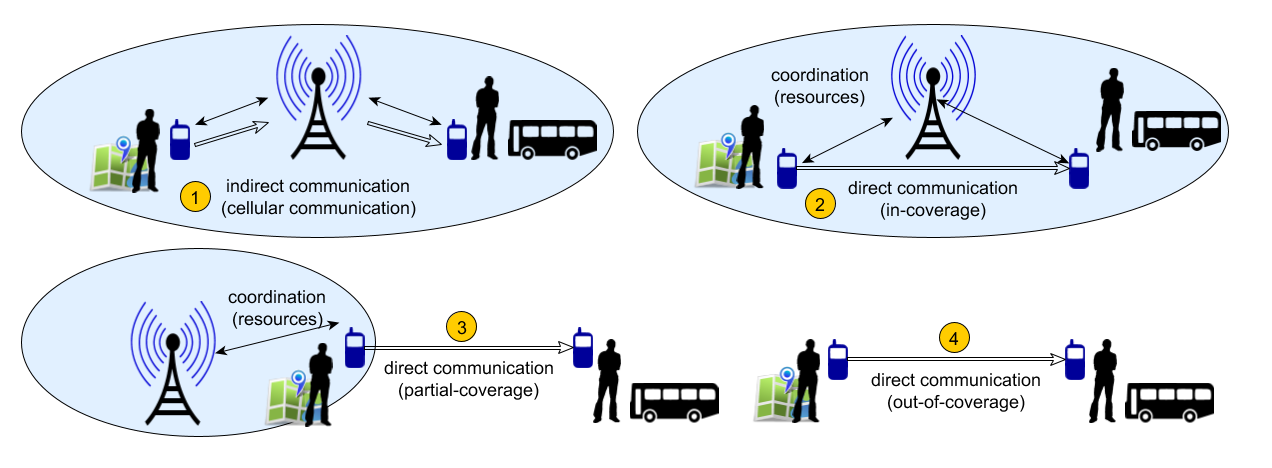
\includegraphics[width=14cm,trim={0 0.5cm 0 0.5cm},clip]{./introduction/directCommunication.png} 
\caption[Cellular communication]{Direct communication in cellular networks. Devices share data via the base station~(1). With direct communication, devices share data directly~(2). Communication is possible even in partial coverage (3) or out-of-coverage (4) scenarios. Usage of the graphic granted by the creator.}
\label{fig:scenarios}
\end{figure}



Direct communication is specified in several mobile standards, whereby two primary technologies have emerged. The first is dedicated short range communication, which is based on WLAN ad hoc networks~\cite{stanley-2023-com}. The first standard was published in 2010 and amended in 2023. The second is `cellular vehicle-to-everything' (C-V2X) communication, which has been developed since the 2010s, gaining more attention through the transition to 5G~\cite{anwar-2019-com}. 
The initial focus of both technologies was on vehicle communication.
However, vehicle and pedestrian traffic differ strongly: People do not move in lanes, their speed is lower, and they can be closer to each other than cars. 
For this reason, 
the \textit{roVer} research project\footnote{The roVer research project (2018-2023) was funded by the German Federal Ministry of Education and Research; grant no. 13FH669IX6. } investigated how direct communication approaches can be transferred to pedestrian traffic. 
Since the technology has not yet been available for smartphones, the simulation framework \textit{CrowNet} was created for the investigations. 
One part of the project focused on mobile communication technology, see~\cite{schuhbaeck-2023-com}. I looked at the sociocybernetics aspects: The crowd and the mobile network form a complex socio-technical system whose interactions must be understood to efficiently manage crowds.
















%%%%%%%






\section{Research field and research question}



Crowd management is an emerging sub-field of pedestrian dynamics research and addresses how crowds can be managed to ensure their safety and comfort. 
While in the early phase of pedestrian dynamics research, the focus was on creating a knowledge base on crowd locomotion -- a prerequisite for managing crowds -- today the focus  is shifting to crowd management: see the recently published books~\cite{otoole-2019-cdyn,silvers-2020-cdyn,feliciani-2021-cdyn,still-2021-cdyn}.
Numerous strategies have been proposed, such as static measures that involve the planning of facilities~\cite{seriani-2015-cdyn,kaakai-2007-cdyn}, placing obstacles~\cite{johansson-2007b-cdyn}, or the provision of evacuation plans~\cite{abdelghany-2014-cdyn}. Such static strategies are efficient when traffic conditions are precisely known in advance. In the case of an unpredictable event, they might fail as they can not adapt. The focus, therefore, shifts to strategies that dynamically intervene using dynamic signs, dynamic obstacles, loudspeaker announcements, auxiliary equipment like robots~\cite{zhou-2019-cdyn}, background music~\cite{zeng-2019-cdyn} or crowd managers on site~\cite{feliciani-2020b-cdyn}.
Another approach to disseminating information is to use mobile applications. There is scarcely any research on how mobile applications can be employed to redirect a crowd except for one single egress experiment~\cite{feliciani-2020-cdyn}. Instead, the pedestrian dynamics community focused on how smartphone usage affects attention and thus movement behavior, see~\cite{echeverria-2023-cdyn,jiang-2018b-cdyn}. 
Apart from that, various crowd sensing approaches~\cite{ribeiro-2023-com,felemban-2014-com,felemban-2020-com,felemban-2021-com,torkamandi-2022-com} have been proposed, employing mobile communication.

However, there is currently no system that senses and automatically informs the crowd based on direct communication technology. I aim to close this gap by developing such a system. My overall goal is to make transportation safer. In many real-life use cases, crowds needed to be guided away from congested or safety-critical areas. Therefore, the system provides route recommendations. To distinguish the system from  navigation systems for individuals, as one knows them for car drivers, I use the term `crowd guidance system' in this thesis. My overarching research question is: How can crowds be redirected through mobile applications based on direct communication technologies? The main question leads to sub-questions on information dissemination, compliance with instructions, and suitable message design.



\vspace{0.2cm}

\phantomsection
\label{reserachquestions}
\begin{tcolorbox}[title=Research question (RQ)]
\textbf{How can crowds be redirected through mobile applications based on direct communication technologies?}

%\vspace{0.1cm}

%Research sub-questions:
\begin{itemize}
\item {Research sub-question (RQ-1):} How reliably are route recommendations disseminated using direct communication in a crowd?
\item {Research sub-question (RQ-2):} Which algorithms are suitable for generating route recommendations for crowds, given not all people follow instructions?
\item {Research sub-question (RQ-3):} How can mobile messages with route recommendations be designed so crowds follow instructions?
\end{itemize}
\end{tcolorbox}








\section{Research methodology}

To answer the research question, I propose and investigate the crowd guidance system step by step. In the course of this, technical and psychological aspects are examined that may affect the performance of a crowd guidance system, see Fig.~\ref{fig:techpsycho}.


\begin{figure}[hbt!]
\centering
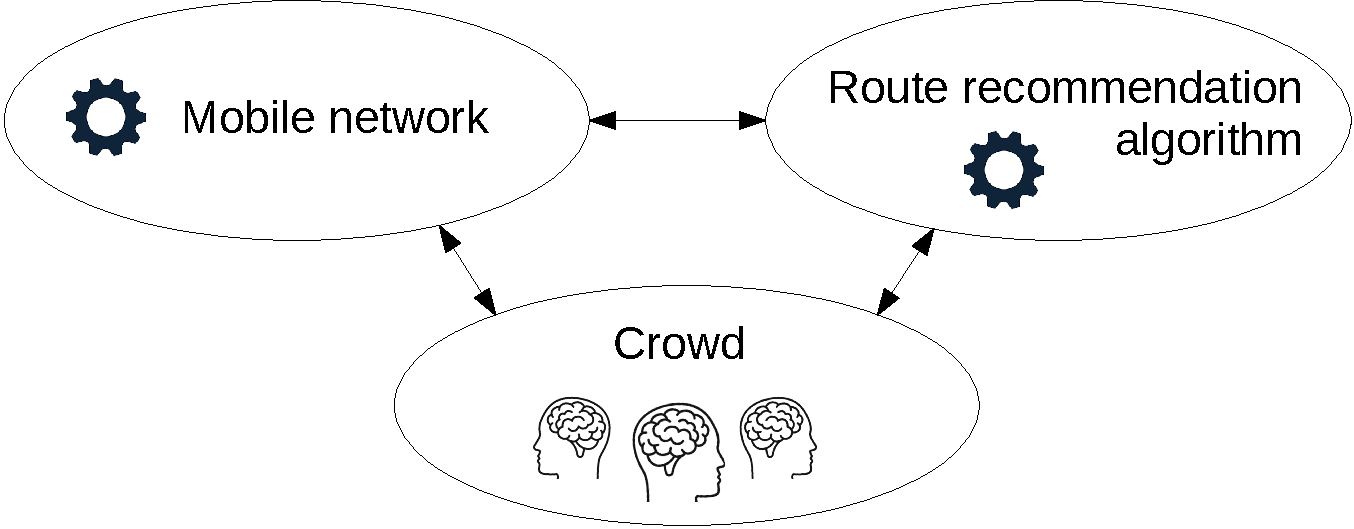
\includegraphics[width=8cm]{../figures/introduction/system.pdf} 
\caption{Components of a crowd guidance system examined in this thesis. I analyze the system from a sociocybernetics perspective, looking at technological and psychological aspects and their interaction.}
\label{fig:techpsycho}
\end{figure}




In step (1), I investigate the suitability of direct communication technology for redirecting mobile crowds. Several studies~\cite{grossglauser-2002-com,bai-2003-com,helgason-2014-com,maccartney-2017-com,chaintreau-2007-cdyn,chancay-2018-com} showed that mobility behavior affects the information dissemination in the mobile network. Crucially, the accuracy of the locomotion model affects the results of the mobile networks simulation~\cite{wischhof-2022b-com}. Many movement models have already been used in network simulations, see the overview~\cite{zhang-2017-com}. Among them are models from the pedestrian dynamics community, such as the Legion Model and the Social Force Model, see~\cite{chancay-2018-com,helgason-2014-com}. So far, only the influence of mobility behavior on the network simulation has been investigated. In a crowd guidance system, however, the mobile network and mobility behavior influence each other bi-directionally: The crowd changes its behavior due to the information disseminated via the mobile network, which, in turn, influences the mobile network.
Such a dynamic system has yet to be investigated. It needs to be clarified how redirection measures affect shadowing and interference, thus, information dissemination in the crowd. My first sub-question therefore asks how reliably redirection information is disseminated in a redirected crowd using direct communication technology, see~\hyperref[reserachquestions]{(RQ-1)}. 



In step (2), I investigate route recommendation algorithms. Meanwhile, numerous guidance approaches have been proposed for crowd management. The algorithms, implemented in the so-called controller, mainly come from engineering. Among them are feedback controllers that aim to affect the locomotion behavior~\cite{kachroo-2010-cdyn, shende-2011-cdyn, shende-2013-cdyn} and controllers trying to influence the decision-making of pedestrians~\cite{zhang-2016-cdyn}. The complexity of these controllers varies greatly from simple On-Off controllers~\cite{gao-2022-cdyn} to more sophisticated methods, such as Model Predictive Control~\cite{menner-2023-cdyn}. 
Unfortunately, most algorithms were developed under unrealistic conditions: It was assumed that the crowd always followed instructions. This is wrong because people may but do not have to follow instructions. Even if they are willing, they may be physically unable or simply not understand what they are supposed to do. I, therefore, find it essential to investigate which algorithms are suitable when not all people follow instructions, see~\hyperref[reserachquestions]{(RQ-2)}.  


In step (3), I investigate how one can improve the compliance of the crowd to follow route recommendations. Studies from communication sciences showed that human behavior can be influenced using message framing, i.e., `presenting logically equivalent options in semantically different ways'~\cite{krishnamurthy-2001-life}. Message framing has been applied in numerous fields like health sciences, marketing, or political communication~\cite{gallagher-2012-life}.  
Techniques from message framing have also been applied to influence crowd behavior: Carter et al.~\cite{carter-2014-life,carter-2015-life} varied the detail of information in a decontamination experiment and found that the crowd complied most when instructions included detailed explanations and instructions. Similar findings have been obtained from studies with individuals~\cite{tormala-2007-life, osman-2018-life}. The communication of information is one factor that can have an impact on behavior. Research from the field of social identity showed that groups and individuals behave differently when group members share a social identity~\cite{reicher-2016-life,carter-2015-life,sivers-2014b-cdyn}.
This can indeed affect the perception of group members~\cite{novelli-2013-life}, and, thus, the decision behavior. Therefore, I want to investigate how message framing can be combined with theory on social identities to find a suitable message design that fosters crowd members to follow route recommendations, see~\hyperref[reserachquestions]{(RQ-3)}.  




I combine methods from computer science, engineering, and the social sciences to answer the main research question and the sub-questions. To investigate the suitability of direct communication in step (1), I model a redirection scenario and conduct a simulation study. I proceed similarly in step (2) to find a suitable route recommendation algorithm. In step (3), an online survey is carried out to assess the effect of message design on route choice. In step (4), I present the complete crowd guidance system, apply it to a real-life use case at the metro station Münchner Freiheit in Munich (Germany), and test it in simulations for which I estimate parameters from the survey data.


\vspace{0.5cm}

\begin{tcolorbox}[title=Proposed methodology for designing a guidance system]
\begin{itemize}
\item[(1)] Test the suitability of direct communication for disseminating route recommendations in a moving crowd $\Rightarrow$~\hyperref[reserachquestions]{RQ-1}. \textit{Method: Modeling \& Simulation}
\item[(2)] Find a suitable route recommendation algorithm $\Rightarrow$~\hyperref[reserachquestions]{RQ-2}. \textit{Method: Modeling \& Simulation}
\item[(3)] Find a message design that convinces crowd members to follow route recommendations $\Rightarrow$~\hyperref[reserachquestions]{RQ-3}.   \textit{Method: Survey}
\item[(4)] Use the findings from (1)-(3) to design and test a proof of concept. $\Rightarrow$~\hyperref[reserachquestions]{RQ}. \textit{Method: Modeling \& Simulation}
\end{itemize}
\end{tcolorbox}

\vspace{0.5cm}




\section{Structure of this work}

The thesis is divided into three main chapters, see Fig.~\ref{fig:leseanleitung}.
Chapter~\ref{sec:state} presents the state of the art on crowd management and approaches for modeling, simulating, and investigating a crowd guidance system. In Chapter~\ref{sec:crownet}, I introduce the novel simulation framework \textit{CrowNet} that was collaboratively developed in the \textit{roVer} research project.
In Chapter~\ref{sec:investigation}, I use this software to investigate my research questions following the proposed methodology. Sections \ref{sec:infoverbreitung}-\ref{sec:reaction} correspond to steps (1)-(3), where I investigate isolated components of a crowd guidance system to answer the research sub-questions. In Section~\ref{sec:realistiscscenario}, I answer the main research question: I propose and test a complete crowd guidance system for a real-life use case at a metro station in Munich (Germany) where football fans need to be guided away from a congested route.


\begin{figure}[hbt!]
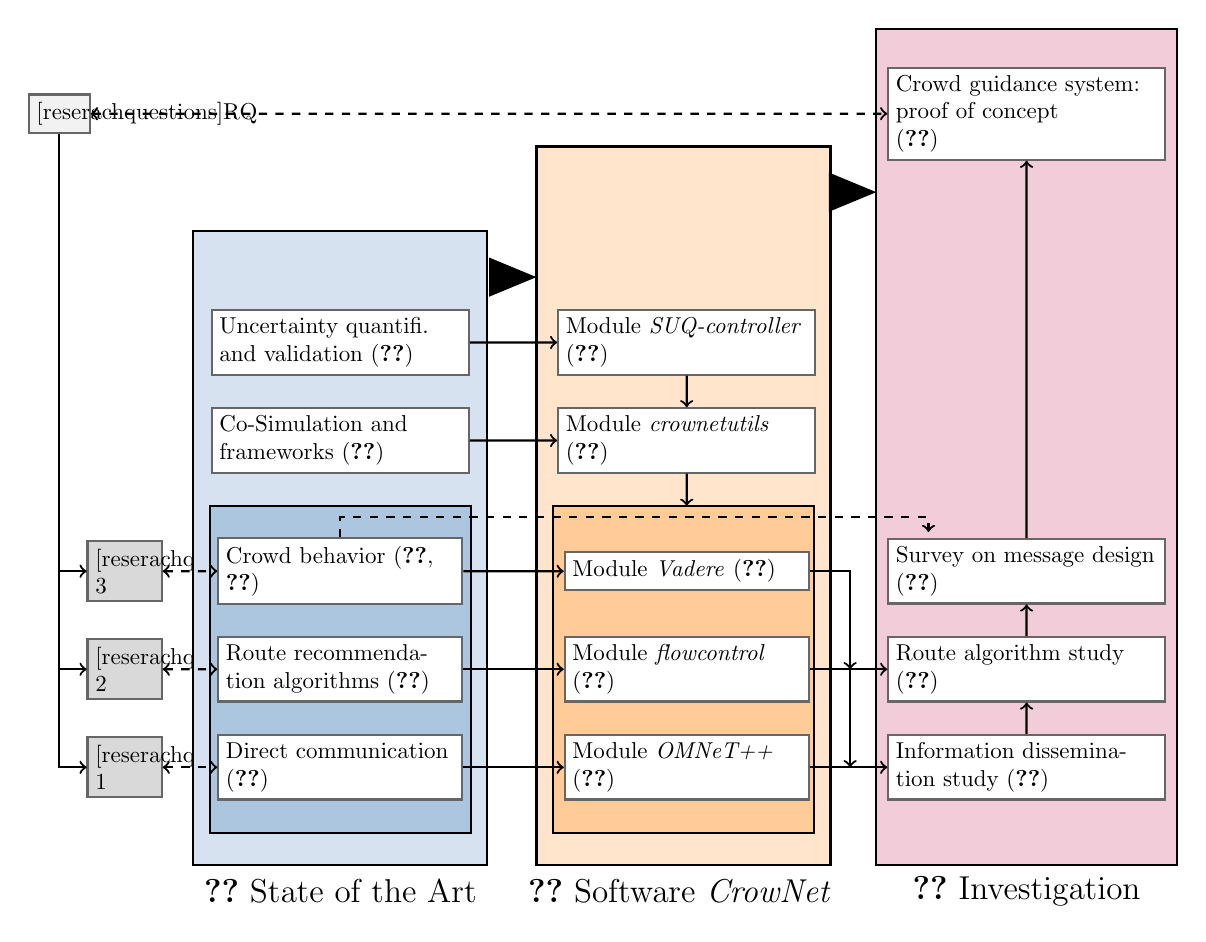
\begin{tikzpicture}[thick,scale=0.83, every node/.style={transform shape}]

\node[rectangle,draw=black!60,fill=gray!30,text width=0.9cm] (a1) at (-3.3,0.0)                            {\hyperref[reserachquestions]{RQ-1}};
\node[rectangle,draw=black!60,fill=gray!30,text width=0.9cm] (b1) at (-3.3,1.5)                            {\hyperref[reserachquestions]{RQ-2}};
\node[rectangle,draw=black!60,fill=gray!30,text width=0.9cm] (c1) at (-3.3,3.0)                            {\hyperref[reserachquestions]{RQ-3}};
\node[rectangle,draw=black!60,fill=gray!10,text width=0.7cm] (rq) at (-4.3,10.0)                            {\hyperref[reserachquestions]{RQ}};

\draw [->] (rq) |- (a1);
\draw [->] (rq) |- (b1);
\draw [->] (rq) |- (c1);



\draw[fill=blue!20] (-2.25,-1.5) rectangle ++(4.5,9.7);
\draw[fill=blue!40] (-2,-1.0) rectangle ++(4,5);

\node[rectangle,draw=black!60,fill=white,text width=3.7cm] (d2) at (0,5.0)                            { Co-Simulation and frameworks (\ref{sec:simulationframeworks})};


\node[rectangle,draw=black!60,fill=white,text width=3.7cm] (e2) at (0,6.5)                            { Uncertainty quantifi. and validation (\ref{sec:uq})};




\node[rectangle,draw=black!60,fill=white,text width=3.5cm] (a2) at (0,0.0)                            { Direct communication  (\ref{sec:modelcom})};
\node[rectangle,draw=black!60,fill=white,text width=3.5cm] (b2) at (0,1.5)                            { Route recommendation algorithms  (\ref{sec:modelalg})};
\node[rectangle,draw=black!60,fill=white,text width=3.5cm] (c2) at (0,3.0)                            { Crowd behavior   (\ref{sec:crowdbah}, \ref{sec:modelcrowd})};

\draw [<->,dashed] (a1) -- (a2);
\draw [<->,dashed] (b1) -- (b2);
\draw [<->,dashed] (c1) -- (c2);

\draw[fill=orange!20] (3,-1.5) rectangle ++(4.5,11);
\draw[fill=orange!40] (3.25,-1.0) rectangle ++(4,5.0);

\node[rectangle,draw=black!60,fill=white,text width=3.5cm] (a3) at (5.3,0.0)                            { Module \textit{OMNeT++} (\ref{sec:omnet})};
\node[rectangle,draw=black!60,fill=white,text width=3.5cm] (b3) at (5.3,1.5)                            { Module \textit{flowcontrol } (\ref{sec:flowcontrol})};
\node[rectangle,draw=black!60,fill=white,text width=3.5cm] (c3) at (5.3,3.0)                            { Module \textit{Vadere}  (\ref{sec:vadere})};


\node[rectangle,draw=black!60,fill=white,text width=3.7cm] (d3) at (5.3,6.5)                            { Module \textit{SUQ-controller } (\ref{sec:suqc})};

\node[rectangle,draw=black!60,fill=white,text width=3.7cm] (e3) at (5.3,5.0)                            { Module \textit{crownetutils} (\ref{sec:crownetutils})};


\draw [->] (a2) -- (a3);
\draw [->] (b2) -- (b3);
\draw [->] (c2) -- (c3);
\draw [->] (d3) -- (e3);
\draw [->] (e2) -- (d3);


\draw[fill=purple!20] (8.2,-1.5) rectangle ++(4.6,12.8);

\node[rectangle,draw=black!60,fill=white,text width=4.0cm] (a4) at (10.5,0.0)                            { Information dissemination study (\ref{sec:infoverbreitung})};
\node[rectangle,draw=black!60,fill=white,text width=4.0cm] (b4) at (10.5,1.5)                            { Route algorithm study (\ref{sec:umleitalgorithmen})};
\node[rectangle,draw=black!60,fill=white,text width=4.0cm] (c4) at (10.5,3.0)                            { Survey on message design (\ref{sec:reaction})};
\node[rectangle,draw=black!60,fill=white,text width=4.0cm] (d4) at (10.5,10.0)                            {Crowd guidance system: proof of concept \\ (\ref{sec:realistiscscenario})};
%\draw [black,
    decorate, 
    decoration = {brace,
        raise=-15pt,
        amplitude=5pt}] (8,-4.5) --  (4,-4.5)
node[pos=0.5,black]{Assembling};
\draw [->] (a4) -- (b4);
\draw [->] (b4) -- (c4);
\draw [->] (c4) -- (d4);

\draw [->] (a3) -- (a4);
\draw [->] (b3) -- (b4);
\draw [->] (c3) -| (7.8,1.5);
\draw [->] (c3) -| (7.8,0.0);

\draw [->,dashed] (c2) |- (9.0,3.83) --  (9.0,3.6) ;



\node[isosceles triangle,
    draw,
    fill=black,
    minimum size =0.55cm] (T)at (2.45,7.5){};
    \node[isosceles triangle,
    draw,
    fill=black,
    minimum size =0.55cm] (T)at (7.65,8.8){};
    
\draw [->] (d2) --  (e3);
\draw [<->,dashed] (rq) -- (d4);

\draw [->]  (e3) -- (5.3,4.0) ;


\node[font=\Large] at (0,-1.9){\ref{sec:state} State of the Art};
\node[font=\Large] at (5.2,-1.9){\ref{sec:crownet} Software \textit{CrowNet}};
\node[font=\Large] at (10.5,-1.9){\ref{sec:investigation} Investigation};

\end{tikzpicture}
\caption[Reading instructions]{Reading instructions. The thesis is divided into three main chapters. The arrows indicate how the research question (\hyperref[reserachquestions]{RQ}) and the sub-questions (\hyperref[reserachquestions]{\mbox{RQ-1}}, \hyperref[reserachquestions]{RQ-2}, \hyperref[reserachquestions]{RQ-3}) are related to the individual chapters and sections. }
\label{fig:leseanleitung}
\end{figure}





\chapter{State of the Art}
\label{sec:state}

This section consists of an application-related part, where I present state-of-the-art approaches and theory on crowd management, and a methods-related part that comprises approaches from computer science for the simulative assessment of a crowd guidance system.


In the first part (Section~\ref{sec:crowdmanagement}), I look at crowd management from a traffic engineering perspective to give an overview of the research field and its application in practice. I identify research gaps that I aim to close in my later investigations. Therefore, the first part is strongly connected to the research questions presented in the introduction. 


In the second part (Sections~\ref{sec:modelcrowd}-\ref{sec:uq}), I look at methodological aspects from a computer science perspective. As I base my investigations on simulations, I look at how the key components of a crowd guidance system, which are the crowd and the mobile network, can be modeled and simulated. In Section~\ref{sec:modelcrowd}, approaches for modeling and simulating crowd behavior are presented. I introduce a hierarchical modeling approach where locomotion is modeled at the operational layer and route choice at the tactical layer. In Section~\ref{sec:modelcom}, I provide an overview of mobile communication standards that specify direct communication and discuss how the respective protocol stacks and the radio channel are modeled and simulated.  
Since crowd and network models are separate models, Section~\ref{sec:simulationframeworks} presents techniques for connecting them. This includes update schemes and techniques for data exchange between simulators. 
It is crucial to quantify errors or uncertainties in the simulation output. Therefore, I present a surrogate-based approach with polynomial chaos expansions in Section~\ref{sec:uq}. 



\section{Crowd Management}

This section belongs to the application-related part of the state of the art. First, crowd management is differentiated from crowd control. Next theory and metrics on crowd safety and comfort are introduced. To foster people's compliance to follow route instructions, I look at theories that describe the psychological behavior of crowds and the aspects of communication. Then I describe approaches for measuring crowd properties. At the end of this section, I give an overview of suggested approaches where guidance signals are automatically generated using algorithms. 


\label{sec:crowdmanagement}

\subsection{What is Crowd Management?}
\label{sec:crowdcontroldef}
\enquote{Crowd management aims for behavioral change by applying information measures, especially to optimize the use of available infrastructural capacity}~\cite{zomer-2015-cdyn}. 
 The term `crowd management' denotes \enquote{proactive security activities that bring safety and comfort to individuals by facilitating efficient movement of crowds}~\cite[p.3]{feliciani-2021-cdyn}.  Crowd management is employed at busy places such as airports, shopping malls, exhibition halls, or train stations and at major events such as concerts or sports competitions~\cite{feliciani-2021-cdyn}.
There are numerous strategies to influence the movement of crowds, which are divided into five levels according to their intensity: inform,  advise, guide, steer, and enforce~\cite{zomer-2015-cdyn,tertoolen-2012-cdyn}, see~Fig.~\ref{fig:fivestages}.
\begin{figure}[hbt!]
\centering
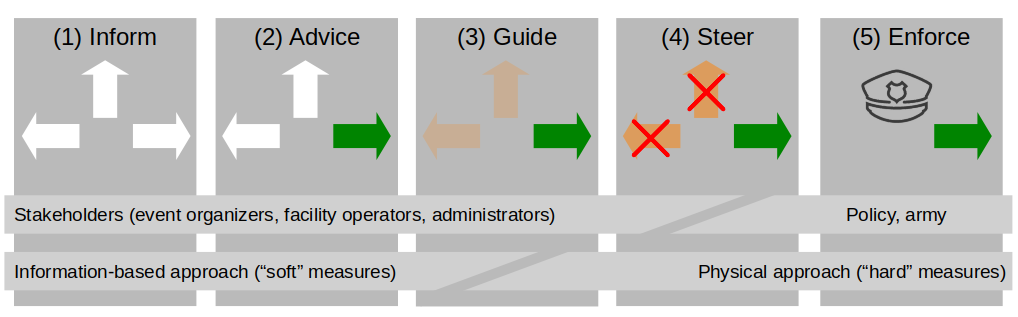
\includegraphics[width=\textwidth]{../figures/state-of-the-art/crowdmanagement/ficestages.png} 
\caption[Strategies for influencing crowd behavior ]{Strategies for influencing crowd behavior. Crowd management uses information-based approaches such as informing and providing advice (1,2). Crowd control employs physical measures to enforce a certain behavior (4,5). Guiding people (3) is located at the transition between the soft (1,2) and the hard (4,5) measures. Own graphic  inspired by \cite[p.168]{feliciani-2021-cdyn}. }
\label{fig:fivestages}
\end{figure}




In the `inform' stage, neutral information is provided using signs, maps, and colored paths. In the `advice' stage, information is manipulated to bias the decision, for example, the naming of walking paths: football fans might favor a walking path to the stadium named after a famous football player. Notably, the crowd is unaware of the manipulation~\cite[p.169]{feliciani-2021-cdyn}. 
In the `guiding' stage, the manipulation is presented obviously to the crowd using instructions that are disseminated through loudspeakers, announcements, information monitors, or light signage.  
The intensity of the measures is higher than in the `advice' stage and can involve low-intense physical measures such as staff blocking a closed gate. The crowd is fully aware of the manipulation.
In the `steer' stage physical measures, like for example placing a barrier, are employed. In this stage, it takes people great effort to defy the measures. In the `enforce' stage, specific behavior is enforced by the police or army using water cannons, tear gas, or brute force. Crowd management corresponds to the stages that aim to inform, advise, and guide~\cite{feliciani-2021-cdyn}. Importantly, people are free to decide whether to follow instructions. Therefore, it is essential to consider the compliance of people when developing a crowd guidance system.





\subsection{Quantitative characteristics of crowds and safety evaluation }
\label{sec:fundamentaldiagram}
 
Crowd and pedestrian behavior can be quantified and evaluated using several measurement quantities and metrics. One of them is the fundamental diagram that describes the relationship between density and flow~\cite{adrian-2019-cdyn}, see Fig.~\ref{fig:fundamental}. The flow increases over the density until the critical density is reached, at which the flow is maximal, that is, the capacity. Beyond the critical density, the flow decreases until the jamming density is reached, and movement is no longer possible.
The density range between $0\,\text{ped/m}^2$ and the critical density is called the free flow regime because there is enough space to allow most pedestrians to walk at their desired speeds~\cite{feliciani-2021-cdyn}. According to the Handbook of Fire Protection Engineering (SFPE)~\cite{hurley-2016-cdyn}, the free flow regime corresponds to a density range $[0\,\text{ped/m}^2, 1.88\,\text{ped/m}^2]$. 


\begin{figure}[hbt!]
\begin{tikzpicture}
\node[] at (0,0) {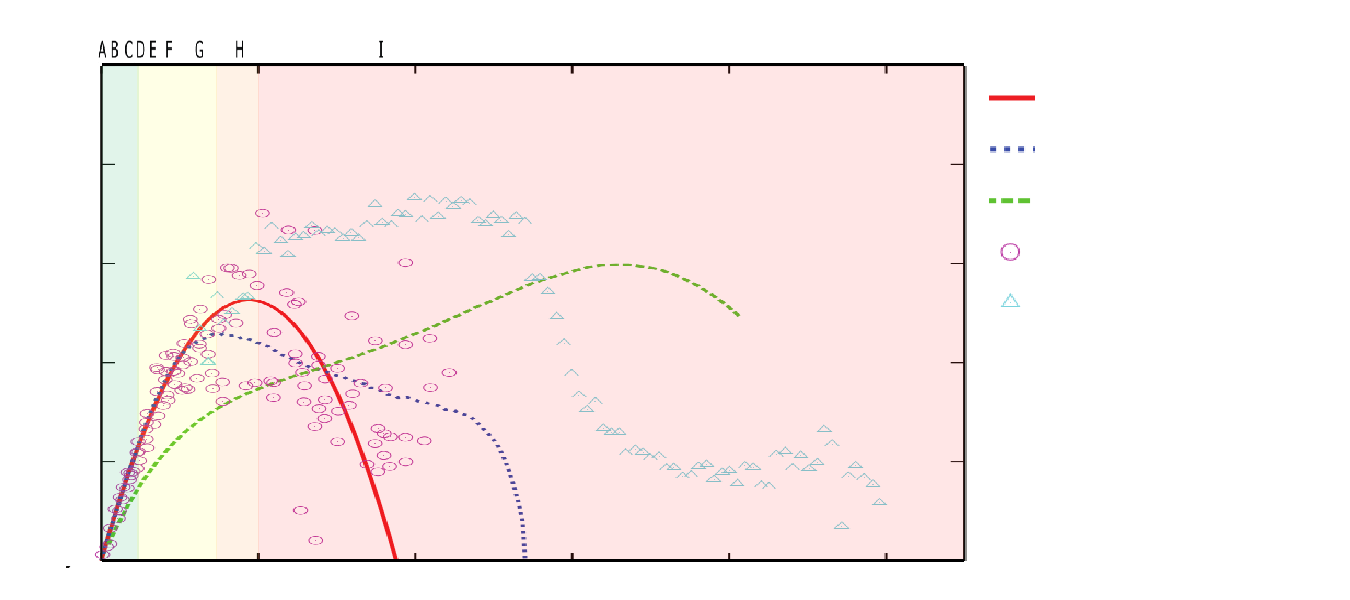
\includegraphics[width=15cm]{../figures/state-of-the-art/crowdmanagement/fundamental_diagram.pdf} };
\node[text width=5cm] at (6.8,2.2) {SFPE~\cite{hurley-2016-cdyn}};
\node[text width=5cm] at (6.8,1.6) {Weidmann~\cite{weidmann-1994-cdyn}};
\node[text width=5cm] at (6.8,1.1) {Predtechenskii~\cite{predtechenskii-1968-cdyn} };
\node[text width=5cm] at (6.8,0.6) {S. Older~\cite{older-1968-cdyn}};
\node[text width=5cm] at (6.8,0.0) { Helbing et al.~\cite{helbing-2007-cdyn} };

\node[text width=5cm] at (-0.8,-3.5) { Crowd density in $peds/m^2$};
\node[text width=5cm,rotate=90] at (-7.2,0.4) { Specific flow in $ped/(ms)$};
\node[text width=8cm] at (1.5,2.8) {  \begin{scriptsize} Level of Service according to Weidmann\end{scriptsize} };

\node[text width=5cm] at (-2,2.2) { Congestion};
\draw[->] (-4.6,1.9) -- (-3.7,1.9);
\draw[dashed] (-4.6,-3) -- (-4.6,2.1);

\node[] at (-6.2,-3.2) { \begin{footnotesize} 0 \end{footnotesize} };
\node[] at (-4.6,-3.2) { \begin{footnotesize} 2 \end{footnotesize} };
\node[] at (-2.9,-3.2) { \begin{footnotesize} 4 \end{footnotesize} };
\node[] at (-1.1,-3.2) { \begin{footnotesize} 6 \end{footnotesize} };
\node[] at (0.6,-3.2) { \begin{footnotesize} 8 \end{footnotesize} };
\node[] at (2.3,-3.2) { \begin{footnotesize} 10 \end{footnotesize} };

\node[] at (-6.7,-2.9) { \begin{footnotesize} 0 \end{footnotesize} };
\node[] at (-6.7,-0.7) { \begin{footnotesize} 1 \end{footnotesize} };
\node[] at (-6.7,1.5) { \begin{footnotesize} 2 \end{footnotesize} };



\end{tikzpicture}
\caption{Fundamental diagram. The flow increases over the density until the maximum flow (capacity) is reached. For higher densities, the flow decreases. The shape of the fundamental diagram differs for the studies~\cite{hurley-2016-cdyn,weidmann-1994-cdyn,predtechenskii-1968-cdyn,older-1968-cdyn,helbing-2007-cdyn} because it depends on several factors, such as age or culture. Own graphic inspired by~\cite{zhang-2012e-cdyn,kitzlinger-2020-cdyn}.}
\label{fig:fundamental}
\end{figure}


As one can observe in Fig.~\ref{fig:fundamental}, the fundamental diagram differs from study because the density-flow-relationship depends on several factors: topological features, such as crossings, stairs~\cite{burghardt-2013-cdyn}, the directionality of flows~\cite{feliciani-2016b-cdyn}, age~\cite{cao-2016-cdyn,ren-2019-cdyn}, religion~\cite{subramanian-2021-cdyn}, and culture~\cite{chattaraj-2009-cdyn}, visibility conditions~\cite{cao-2018-cdyn}, the motivational level~\cite{ye-2012-cdyn}, environmental conditions such as the temperature~\cite{kim-2018-cdyn}, and the measurement method~\cite{zhang-2012e-cdyn}. For an overview of factors, I refer to~\cite{paetzke-2023-cdyn}.

Important for crowd management applications is that the location and size of the measurement area have an influence:  The maximum density cannot be measured in the center of a bottleneck but in front of it~\cite{zhang-2012e-cdyn}. Also, the larger the area, the smoother the density measurements.



To describe the relationship between flow and density analytically, numerous models have been proposed, see e.g.~\cite{hurley-2016-cdyn,mori-1987-cdyn,bosina-2018-cdyn,fruin-1971-cdyn,lam-1995-cdyn,navin-1969-cdyn}. In the pedestrian dynamics community, the Kladec equation~\cite{weidmann-1992-cdyn} is widely used that relates the specific flow $J_s$ to the density $\rho$:
\begin{equation}
J_s = \rho v_0  \left( 1  - e^{-1.913 \left(  \frac{1}{\rho} - \frac{1}{\rho_{\text{jam}}} \right) }  \right)
\label{eq:kladec}
\end{equation}
with the jamming density $\rho_\text{jam}=5.4\,\text{ped/m}^2$ and the free flow velocity $v_0=1.34\,\text{m/s}$ according to Weidmann~\cite{weidmann-1992-cdyn}.


\subsubsection{Congestion definition based on the fundamental diagram}
The definition of congestion is an ongoing topic within the pedestrian dynamics community. Currently, no standardized definition is available. Compare, for example, the definitions in~\cite{rimea-2016-cdyn} and~\cite{kitzlinger-2020-cdyn}.
Kitzlinger et al.~\cite{kitzlinger-2020-cdyn} suggest defining congestion based on the fundamental diagram: Congestion is present when the capacity is exceeded, or, in terms of flows, jamming occurs if the inflow is larger than the capacity. This criterion is identical to the jamming criterion proposed in~\cite{schadschneider-2009-cdyn,zhang-2011-cdyn}. 
In terms of densities, this means that the density must stay below the critical density.

There are several values suggested for the critical density: $1.75\,\text{ped/m}^2$ according to Weidmann~\cite{weidmann-1994-cdyn}, $2.16\,\text{ped/m}^2$ according to Fruin~\cite{fruin-1971-cdyn}, $1.88\,\text{ped/m}^2$ according to the Handbook of Fire Protection Engineering~\cite{hurley-2016-cdyn} and $6.64\,\text{ped/m}^2$ according to Predtechenskii~\cite{predtechenskii-1968-cdyn}. Except from the study in~\cite{predtechenskii-1968-cdyn}, the critical density is always around $2\,\text{ped/m}^2$ which aligns with the qualitative observations of Oberhagemann~\cite{oberhagemann-2012-cdyn}. Therefore, this value is a suitable threshold for crowd management applications.

\subsubsection{Level of service: Basis for safety evaluation}

The Level of Service (LOS) qualitatively describes the movement behavior of a crowd. The density is divided into levels, each qualitatively describing a certain movement behavior, see Tab.~\ref{tab:levelofservice}. Therefore, it is used to evaluate safety and comfort. 

Like the fundamental diagram, the qualitative movement behavior depends on numerous factors, which is why different level of service schemes have been proposed~\cite{yadav-2024-cdyn}. In crowd management applications, the categorizations according to Fruin~\cite{fruin-1971-cdyn} and Weidmann~\cite{weidmann-1994-cdyn} are typically used, see~Fig.~\ref{fig:fruinweidmann}. 



\begin{table}[hbt!]
\centering
Level of Service according to Fruin~\cite{fruin-1971-cdyn}
\begin{tabular}{p{1.0cm}p{8.5cm}p{1.5cm}p{1.5cm}}
\hline 
Level  & Walking behavior &Density $\text{ped/m}^2$ & Flow $\text{ped/m/min}$  \\ 
\hline
A & Pedestrians walk with their desired speed &  $<0.31$ & $<23.0$  \\ 
B & Occasionally interference with other pedestrians & $<0.43$ & $<30.5$ \\ 
C & Partially reduced walking speed & $<0.72$ & $<49.2$   \\ 
D & Rare passing maneuvers & $<1.08$ & $<65.6$  \\ 
E &Temporal stops, no passing maneuvers     & $<2.17$ & $<82.0$  \\ 
F &Physical contact between crowd members  &  $\geq 2.17$ & $ \geq 82.0$   \\ 
\hline 
\end{tabular} 
\caption[Level-of-Service concept for pedestrian traffic]{Level-of-Service levels for pedestrian traffic according to Fruin~\cite{fruin-1971-cdyn}. Density and flow values are only valid for walkways. The best category is the A level, where the density and flow are the lowest.}
\label{tab:levelofservice}
\end{table}



\begin{figure}[hbt!]
\centering
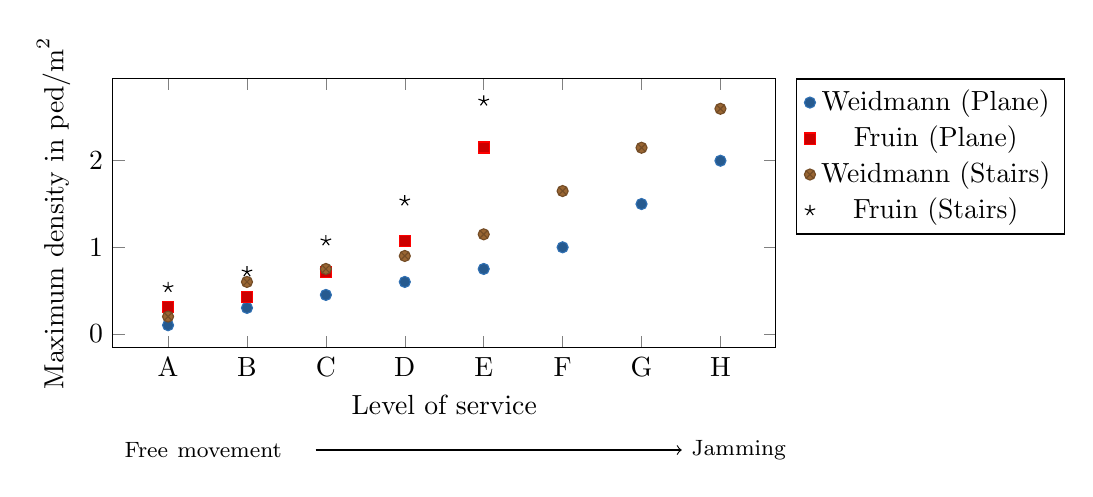
\begin{tikzpicture}
\begin{axis}[xlabel=Level of service,legend entries={Weidmann (Plane), Fruin (Plane),  Weidmann (Stairs), Fruin (Stairs)}, legend pos=outer north east, ylabel={Maximum density in $\text{ped/m}^2$},width=10cm,height=5cm, xtick={1,2,3,4,5,6,7,8}, 
  xticklabels={A,B,C,D,E,F,G,H},]
\addplot+ [only marks] table [] {
x y
1 0.1
2 0.3
3 0.45
4 0.6
5 0.75
6 1.0
7 1.5
8 2.0
};
\addplot+ [only marks] table [y expr=10.7639150512/\thisrow{y}] {
x y
1 35
2 25
3 15
4 10
5 5 Oberhagemann \cite{oberhagemann-2012-cdyn} haben Einteilungen vorgeschlagen.

};
\addplot+ [only marks] table [] {
x y
1 0.2
2 0.6
3 0.75
4 0.9
5 1.15
6 1.65
7 2.15
8 2.6
};
\addplot+ [only marks] table [y expr=10.7639150512/\thisrow{y}] {
x y
1 20
2 15
3 10
4 7
5 4
};
\end{axis}
\node[text width=2.3cm] (a) at (1.3,-1.3) {\begin{footnotesize}Free movement\end{footnotesize}};
\node[text width=2.3cm] (c) at (8.5,-1.3) {\begin{footnotesize}Jamming \end{footnotesize}};
\draw[->] (a) -- (c);

\end{tikzpicture}
\caption{Upper density bounds of the Level-of-Service concepts according to Weidmann~\cite{weidmann-1994-cdyn} and Fruin~\cite{fruin-1971-cdyn}. For each level the maximum density is depicted for walkways (`Plane') and stairs. The higher the level, the stronger the maximum densities differ (A is the lowest level). One can observe that Weidmann's classification~\cite{weidmann-1994-cdyn} is more rigorous than Fruin's~\cite{fruin-1971-cdyn}: The blue and brown data points are always below the red and black data points.  }
\label{fig:fruinweidmann}
\end{figure}

Weidmann~\cite{weidmann-1994-cdyn} divides the density into nine levels depending on the traffic situation, assigning them levels A (best level) to I (worst level). Free movement in the plane is present at densities $<0.1\,\text{ped/m}^2$, which corresponds to level A~\cite[p.97]{weidmann-1994-cdyn}. In Level I, the density $>2\,\text{ped/m}^2$ which means there is 'massive crowding'~\cite[p.97]{weidmann-1994-cdyn}. 

Fruin distinguishes only six levels: A-F. The A level describes a free-flow situation, while the F level describes a standstill situation, see Tab.~\ref{tab:levelofservice}. Like Weidmann~\cite{weidmann-1994-cdyn}, Fruin~\cite{fruin-1971-cdyn} adjusts the density and flow intervals depending on the scenario. For walking in the plane and for stairs, the density maximal density for each level differs strongly, see again Fig.~\ref{fig:fruinweidmann}. 

\subsubsection{Evaluation of safety and comfort}
\label{sec:risk}

Safety and comfort are evaluated using flow or density-based criteria. Several recommendations are available that are based on the level of service concept: Weidmann~\cite{weidmann-1994-cdyn} recommends a B level for walkways in general. A level D is only acceptable during the rush hour  and a level F is acceptable in bottlenecks where people do not stay a long time~\cite{weidmann-1994-cdyn}. The Highway Capacity Manual~\cite{hpc-2022-cdyn} provide recommendations based on the level of service concept according to Fruin~\cite{fruin-1971-cdyn}: at least a level E should be achieved which is similar to the jamming criterion.

The Pedestrian Comfort Level~\cite{tfl-2019-cdyn} is a flow-based metric for evaluating comfort.
The recommended level depends on the scenario because it is assumed that pedestrians' perception is scenario-specific. In tourist areas where people are likely to spend time voluntarily, people might be particularly sensitive to crowding. In this case, a maximum flow of $11\,\text{ped/min/m}$ is recommended. For a transfer scenario at a train station where commuters stay just a short time, a flow of  $17\,\text{ped/min/m}$ is acceptable, see Fig.~\ref{fig:pedcomfortlevel}.




\begin{figure}[hbt!]
\centering
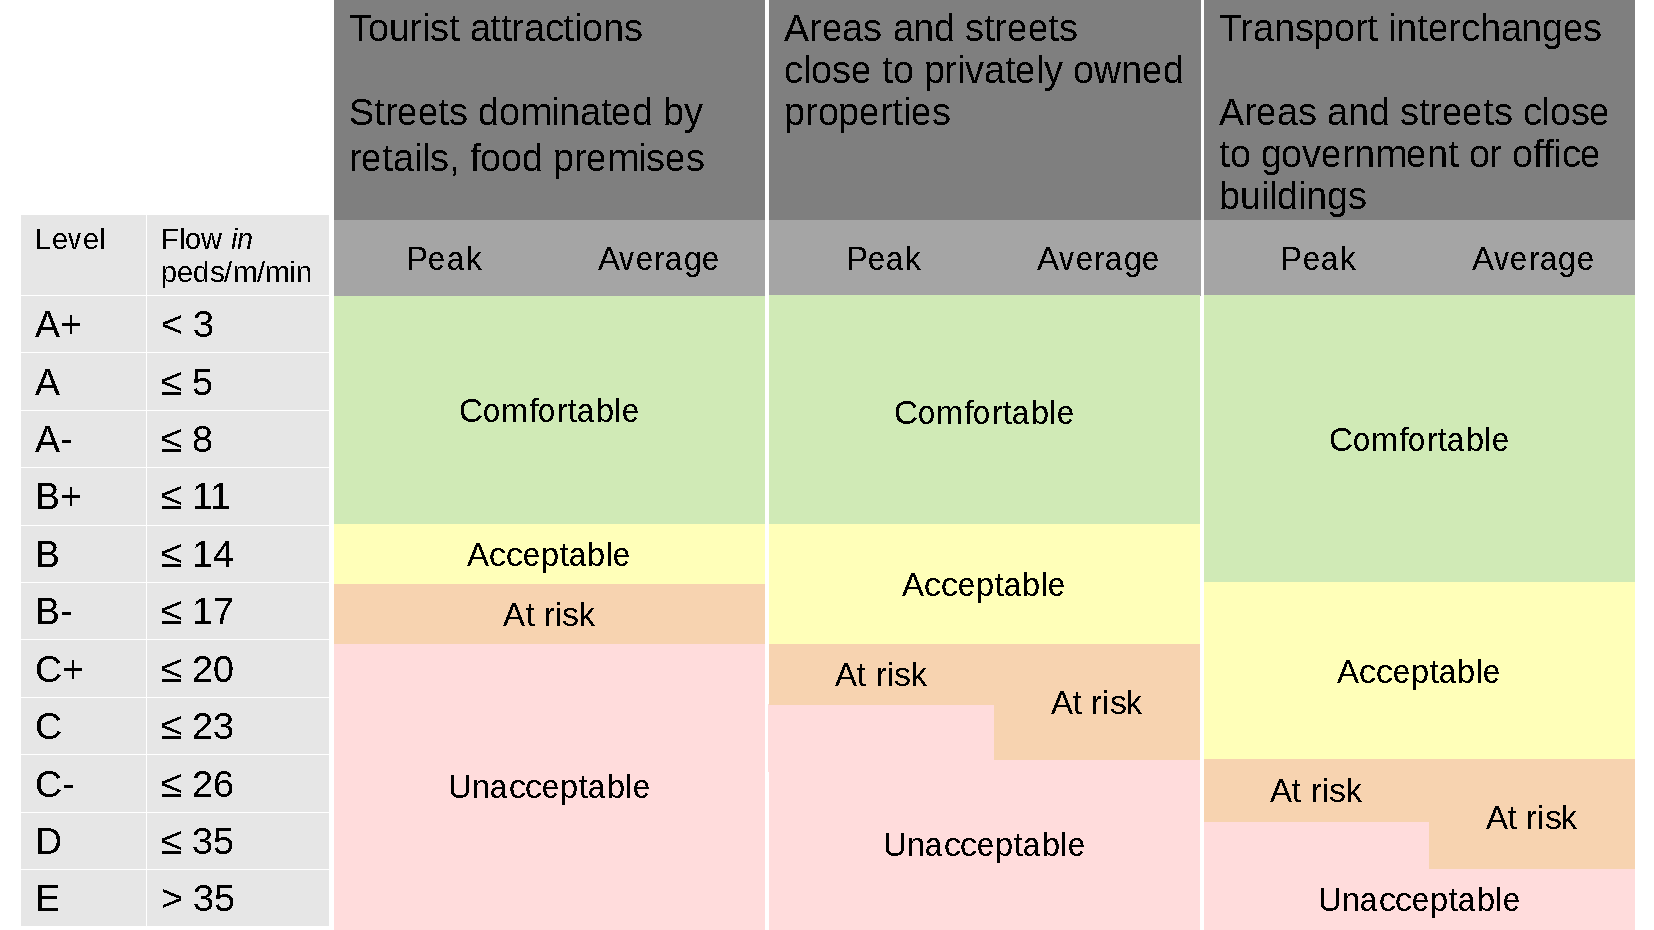
\includegraphics[width=12.5cm]{../figures/state-of-the-art/crowdmanagement/pcl.pdf} 
\caption[Pedestrian Comfort Levels for different traffic scenarios]{Pedestrian Comfort Levels for different traffic scenarios. It is assumed that people experience comfort scenario-specifically: They are more sensitive to crowding in tourist areas, where they spend their spare time, than at train stations where they only pass a short time for traveling. Own graphic based on the recommendations from~\cite{tfl-2019-cdyn}.}
\label{fig:pedcomfortlevel}
\end{figure}



Finally, I would like to address so-called safety indices~\cite{carter-2007-cdyn,zegeer-2006-cdyn,montella-2020-cdyn,krishnan-2023-cdyn}, as I have repeatedly come across these metrics in my literature research.
Safety indices are used in traffic engineering to compare traffic scenarios within a city. With this, a traffic engineer can identify the most safety-critical spots for improving traffic. However, these indices are unsuitable for crowd management because they only compare but do not evaluate safety. 



\subsection{Key theories on crowd behaviour}
\label{sec:crowdbah}


A prerequisite for the development of crowd management applications is understanding crowds' behavior. 
Several theories have been proposed to explain the psychological behavior of crowds~\cite{lebon-1895-life,freud-1921-life,allport-1924-life,zimbardo-1999-life,sherif-1936-life,turner-1957-life,berk-1974-life,berk-1974a-life}. One can distinguish between classical and modern theories. Classical theories only explain violent behavior but cannot explain peaceful gatherings, so these theories are regarded as outdated~\cite{challenger-2009-cdyn}. Since modern theories have emerged from these, I find it essential to be familiar with their basic principles, so I briefly list the key ideas in Tab~\ref{tab:classicaltheories}.



\begin{table}[hbt!]
\begin{tabular}{p{4cm}p{10cm}}
 \hline
Classical theory & Basic idea \\ \hline
Le Bon's Group Mind Theory (1895)  \cite{lebon-1895-life} & Individuals lose their sense of self in a crowd and become anonymous. The actions of the crowd are driven by a group mind controlled by primitive instincts. Therefore, crowds are disruptive by nature.  \\ 
Theory according to Freud (1921)  \cite{freud-1921-life} & Individuals' super-ego is surpassed when they are in a crowd which unlocks their unconscious mind. Therefore, individuals are driven by their instincts.  \\
 Individualism Theory (1924)  \cite{allport-1924-life} & Crowd violence is caused by violent predispositions of individuals. Predispositioned individuals reinforce each others' behavior, which aggregates violent behavior. \\
 Deindividuation Theory (1952-1989)  \cite{zimbardo-1999-life} & The anonymity of the crowd members controls the behavior. Individuals lose their self-awareness. The resulting anonymity causes antisocial behaviors.\\
 \hline
\end{tabular}
\caption{Classical theories on crowd behavior. These theories explain violent behavior of crowds but cannot explain peaceful gatherings.   }
\label{tab:classicaltheories}
\end{table}

\subsubsection{Modern crowd theories}

Modern crowd theories aim to explain crowd behavior more generally than classical theories.
The \textit{Theory of Social Norms} (1936)~\cite{sherif-1936-life} introduces the concept of social norms. \enquote{When a group of individuals faces a new unstable situation
and has no previously established interests or opinions regarding the situation, the result is not chaos; a common norm arises, and the situation is structured in relation to the
common norm}~\cite[p.111]{sherif-1936-life}. 
%
The \textit{Emergent Norm Theory} (1957-1964)~\cite{turner-1957-life} extends the concept of social norms. Through interactions, individuals develop new behavioral norms.
%
The \textit{Game Theory} (1972-1974)~\cite{berk-1974-life,berk-1974a-life} assumes that crowds act rationally. Individuals perform actions they believe bring the highest payoff. Crowd members seek information from which they predict possible events. Depending on the reward, the actions are derived, starting with the action that maximizes the reward. Since the reward is difficult to determine in advance, the theory lacks of applicability.
%
The \textit{Place Scripts Theory} (1992)~\cite{donald-1992-life} suggests that individuals follow behavioral patterns. The sequence of actions is called the script. Each action is associated with a certain place. \enquote{They define, understand, or formulate a script in relation to where they are and interpret the behavior of others.}~\cite{donald-1992-life}. According to the theory, familiarity with the environment is disadvantageous in emergency situations, which might not be always the case in reality. %
The \textit{Self-categorization Theory} explains how individuals view themselves in relation to other individuals as a group and how the view of an individual changes when they become a group member. It is based on the meta-contrast principle: Group members perceive strong similarities between themselves and other group members and large differences between themselves and non-group members~\cite{turner-1994-life}.
The \textit{Social Identity Theory}~\cite{tajfel-1974-life,tajfel-1979-life,tajfel-1982b-life,turner-1972-life,turner-1981-life,turner-1982-life,turner-1987c-life} explains how an individual's behavior is influenced by a social identity to a group or crowd, which in turn influences collective behavior. The extent of the sense of belonging is also referred to as the degree of social identification~\cite{templeton-2020-life}. An example is a group of football fans who identify themselves as football fans. The assumption is that exactly one of a person's social identities is salient at a time: For the football fan only the fan identity is salient. Other identities such as being an academic or a painter do not have an effect.

The \textit{Social Identity approach} combines the self-categorization theory with the social identity theory~\cite{templeton-2020-life}.
It is supported by empirical evidence from numerous experiments that demonstrate the effect of social identities on decision-making and movement behavior. 
In-group members who share a social identity are more strongly influenced by members of their social group (in-group members) than by non-group members~\cite{levine-2005-life,carter-2015-life,reicher-2016-life,sivers-2014b-cdyn}. Non-group members are members of an opposing social group, e.g., football fans of the opposing team or people whose group membership is unknown. Sharing a social identity affects the behavior: It was observed that people are more likely to help each other when sharing a social identity~\cite{levine-2005-life}. Consequently, social identities can reinforce positive characteristics and behavior.  Negative emotional responses become weaker: One example is that less disgust is perceived within a group compared to non-group members~\cite{reicher-2016-life}. Social identities also influence mobility behavior. Group members tolerate dense situations more likely and might even enjoy  staying in denser and more central parts of the crowd~\cite{novelli-2013-life}. They also move slower than individuals and stay closer together~\cite{templeton-2018-cdyn}. 
Also, different formations have been observed for groups:  walking next to each other, walking in line, or forming a V-shape~\cite{gorrini-2014-cdyn, koster-2011b-cdyn, moussaid-2010-cdyn, qiu-2010-cdyn,subramanian-2022-cdyn}. 

\subsubsection{Communication with crowds}


For the categorization of communication strategies, a basic understanding of the elements of the communication process is necessary. Therefore, I briefly introduce Berlo's communication model~\cite{berlo-1960-life} which focuses on the components of the communication process. I used them as categories in my literature research. 

Berlo's model~\cite{berlo-1960-life} is composed of a sender, a message, a channel, and a receiver, see Fig.~\ref{fig:commmodel}. 
Senders encode their thoughts into a message that is transmitted over a communication channel. The receiver perceives the message and decodes the information. Several factors, such as the socio-cultural background, the structure and content of a message, or the channel, influence the communication process. Studies in the field of crowd management mainly focus on the channel, testing the suitability of instructions from personnel~\cite{feliciani-2020b-cdyn}, background music~\cite{zeng-2019-cdyn}, or auxiliary equipment, such as robots~\cite{zhou-2019-cdyn}, for the provision of information. There is scarcely any research on employing mobile applications and smartphones for guiding crowds except for one experiment in which a crowd received instructions via their smartphones to accelerate evacuation from a room with four exits~\cite{feliciani-2020-cdyn}.







\begin{figure}[hbt!]
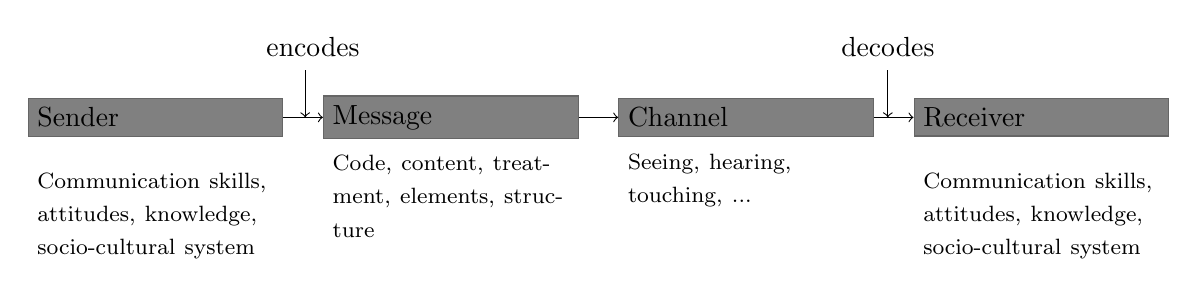
\begin{tikzpicture}

\node[rectangle,draw=black!60,fill=gray,text width=3.0cm] (a) at (0,0.0)                            { Sender };
\node[rectangle,draw=black!60,fill=gray,text width=3.0cm] (b) at (3.75,0.0)                            {Message };
\node[rectangle,draw=black!60,fill=gray,text width=3.0cm] (c) at (7.5,0.0)                            {Channel };
\node[rectangle,draw=black!60,fill=gray,text width=3.0cm] (d) at (11.25,0.0)                            {Receiver };
\draw[->] (a) -- (b);
\draw[->] (b) -- (c);
\draw[->] (c) -- (d);

\draw[->] (1.9,0.6) -- (1.9,0);
\node at (2,0.9) {encodes};

\draw[->] (9.3,0.6) -- (9.3,0);
\node at (9.3,0.9) {decodes};

\node[text width=3.0cm] (a) at (0,-1.25)                            { 
\begin{footnotesize}Communication skills,
attitudes, knowledge, socio-cultural system
\end{footnotesize}
 };
\node[text width=3.0cm] (b) at (3.75,-1.0)                            {\begin{footnotesize}Code, content, treatment, elements, structure
\end{footnotesize} };
\node[text width=3.0cm] (c) at (7.5,-0.8)                            {\begin{footnotesize}Seeing, hearing, touching, ... \end{footnotesize} };
\node[text width=3.0cm] (d) at (11.25,-1.25)                            {\begin{footnotesize}Communication skills,
attitudes, knowledge, socio-cultural system
\end{footnotesize} };

\end{tikzpicture}
\caption{ Components and factors of the communication process. Own graphic of Berlo's communication model proposed in~\cite{berlo-1960-life}.}
\label{fig:commmodel}
\end{figure}


Numerous theories and experimental studies aim to understand how information can be efficiently communicated to crowds in emergencies.  Reynolds et al.~\cite{reynolds-2005-life} provide a theoretical basis by introducing the Crisis and Emergency Risk Communication Model that defines communication activities for different phases of a disaster. 
Drury et al.~\cite{drury-2009-life} conducted a virtual reality experiment where participants imagined being at a metro station when a fire breaks out. They found that people helped each other more often when they shared a social identity. 


Reicher et al.~\cite[p.16]{reicher-2004-life} stress the necessity of communication in conflicts: \enquote{[...] it becomes increasingly important to communicate with the crowd where one seeks to avoid a potentially conflictual relationship, but in situations where relationships are potentially conflictual, crowd members are least likely to trust what the police have to say}. 
Also, it is suggested to use mediators that are trusted and respected within the crowd~\cite{reicher-2004-life}. 
Other studies focus on the design of signage that assesses where and how signs should be placed~\cite{farr-2012-life}. 

Palttala et al.~\cite{palttala-2012-cdyn} suggest employing several communication strategies at once to address heterogeneous crowds.
Van der Wal et al.~\cite{wal-2021-life} found that "dynamic emergency exit floor lighting and staff guiding people to exits were only beneficial for high-density crowds and those unfamiliar with the environment". 
%

Numerous studies from the communication sciences investigate how the message content affects decision behavior. In particular, the quantity and quality of information are analyzed: how much information is necessary? In which way should a particular piece of information be presented? The latter includes the so-called message framing, i.e., `presenting logically equivalent options in semantically different ways'~\cite{krishnamurthy-2001-life}.
%
Message framing plays a role in numerous fields of application. 
In some studies, message framing did not have any effect: Carfora et al.~\cite{carfora-2022b-life} found that the message components `..., you will feel more energetic' and  `..., you will feel less tired' were equally effective in persuading people to switch to a particular diet. Capps at al.~\cite{capps-2022-life} tested the effect of message framing on sanitizer usage during the Covid-19 pandemic. They put different signage next to sanitizers with three different messages: (1) `Using hand sanitizer means you're doing your part to fight the spread of COVID-19 ... Stay healthy!', (2) `Many people use hand sanitizer to fight the spread of COVID-19 ... Join them!', and (3) `More and more people are using hand sanitizer to fight the spread of COVID-19 ... Join them!'. They could not find a statistical difference in sanitizer usage. 

Other studies provide strong evidence that message framing indeed affects the behavior: Nobel~\cite{nobel-2022-life} investigated how message framing can affect peoples' decision to quit smoking. He found that messages that emphasize the financial gain from cigarette cost savings are more effective than loss-oriented messages, such as `if you continue to smoke, you will lose money'. Moreover, he found that addressing the financial advantage is more effective than addressing health aspects such as longevity `if you quit smoking, you will live longer'.
%
In some of the studies the amount of information and number of instructions was varied: Carter et al.~\cite{carter-2014-life,carter-2015-life} conducted studies on mass decontamination and found that the highest level of compliance was achieved when the public was provided with both health-focused information and practical information.
Osman et al.~\cite{osman-2018-life} found that health-related information about smoking increases the tendency to advocate regulations on smoking.
Several other studies exist in which message framing was tested for a particular purpose, see the overview in~\cite{gallagher-2012-life}. 

The examples from my literature research show that message framing can indeed influence behavior of individuals and crowds. 
However, it depends on the use case and the wording whether message framing is particularly effective. It is unclear how message framing can be employed via mobile applications in a crowd guidance system. 
It is, therefore, necessary to investigate how redirection recommendations should be phrased to foster compliance.











\subsection{Pedestrian and crowd sensing technologies}

Crowd-sensing is the task of measuring at least one crowd characteristic~\cite{teixeira-2010-cdyn}:
\begin{itemize}
\item Presence: Is someone present?
\item Count: How many people are present? 
\item Location: How are pedestrians distributed in a space?
\item Track: How do pedestrians move?
\item Identity: Who are the pedestrians?
\end{itemize}


\subsubsection{Visualization-based approaches}
Several technologies are available to detect, count, track, and monitor pedestrians and crowds.
\enquote{One of the most commonly employed solutions to count, track, and analyze pedestrian
activity in public spaces is the use of images from (surveillance) cameras}~\cite[p.79]{feliciani-2021-cdyn}. Optical cameras, thermal cameras, and LiDar-based systems are categorized as visualization-based technologies. All visualization-based approaches have in common that crowd characteristics are derived from image data for which computer vision or machine learning techniques are used, see Tab.~\ref{tab:verfahrenbildinfo}.
 
 
\begin{table}[hbt!]
\centering
\begin{tabular}{llll}
\hline 
Image descriptors & Classifiers \\ \hline
Histogram of oriented gradients &  Support vector machines \\ %& pixel-based procedure that divides the image into cells and estimates gradient directions and edge orientations, used for object detection \\ 
Local Binary Pattern  & Neuronal Networks  \\ % classifier, used in combination with the Histogram of oriented gradients descriptor \\
Haar-like feature  & Gaussian (Mixture) Model \\ %uses Haar wavelet representations for face recognition; does not consider motion  \\
Viola-Jones feature & ... \\
... &  \\ % & uses Haar wavelets and particle filters for dynamic face recognition \\
%& Discriminative deep model based on Restricted Boltzmann Machine (RBM) building blocks  & \\
 \hline
\end{tabular} 
\caption{Examples of image descriptors and classifiers used to gain information about a crowd from images. Application examples can be found in~\cite{brunetti-2018-cdyn}.}
\label{tab:verfahrenbildinfo}
\end{table} 




\subsubsection{Non visualization-based approaches}
Non-visualization-based technologies estimate crowd properties by using radio signals, temperature, or sounds, see Fig.~\ref{fig:classification}. The approaches can be classified as device-free or device-based.


\begin{figure}[hbt!]
\centering
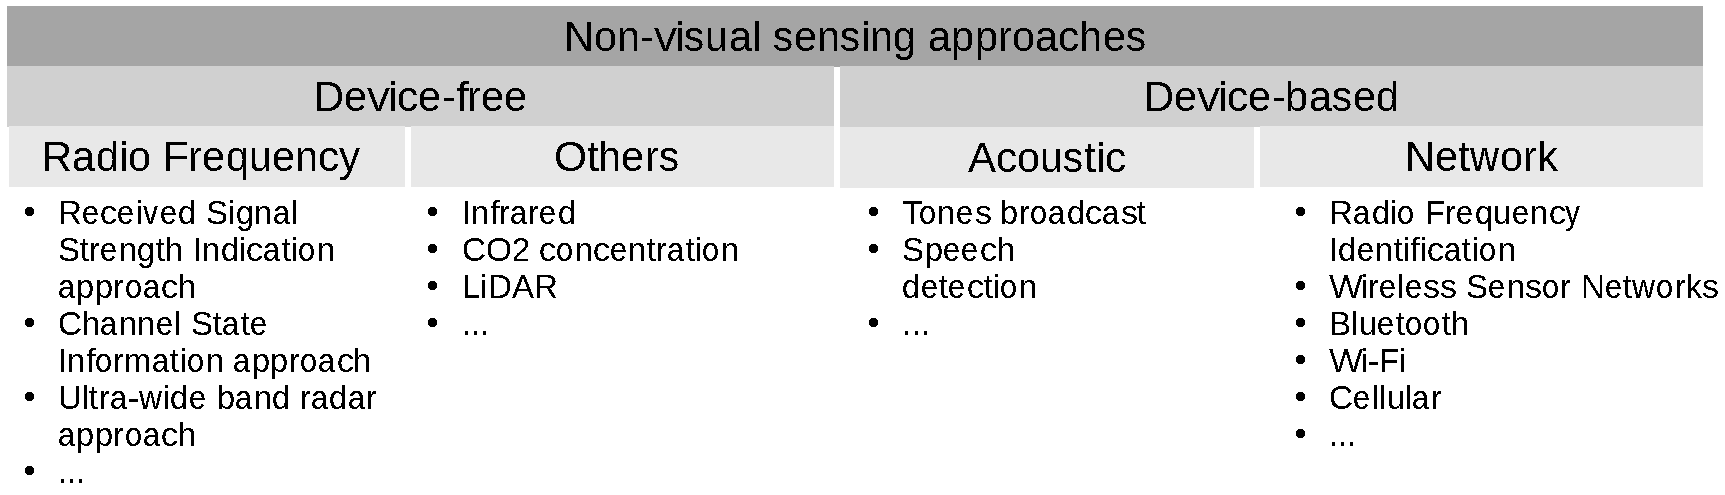
\includegraphics[width=0.9\textwidth]{../figures/state-of-the-art/crowdmanagement/sensing_nonvisual.pdf} 
\caption[]{Categorization of non-visualization-based sensing technologies. Own \mbox{graphics} inspired by~\cite{kouyoumdjieva-2019-cdyn}.  }
\label{fig:classification}
\end{figure}
%



Device-free approaches do not require crowd members to carry special sensors or devices~\cite{kouyoumdjieva-2019-cdyn}. Some of these device-free approaches employ the radio frequency band. In the \textit{Received Signal Strength Indication} approach, the sensor measures the power of a radio signal of a known radio infrastructure node such as WLAN access point. Since pedestrians hinder wave propagation, it is assumed that the number of pedestrians is high when the power is low and vice versa. The same principle is used in the \textit{Channel State Information} approach. Here, however, signals are transmitted on multiple frequencies (OFDM), which allows the power level and, thus, the number of people to be determined more precisely~\cite{wu-2012-com}.
So-called \textit{ultra-wide band} radar sensors also work with radio frequencies. They estimate the number of people by emitting an impulse signal and analyzing its reflection~\cite{choi-2017-com}. 
%
Some other approaches do not use the radio band. These include \textit{infrared} sensors, which correspond to the industry standard among device-free methods~\cite{kouyoumdjieva-2019-cdyn}. They either detect the body temperature (pyroelectric infrared sensor) or act as a light barrier: when the light beam is interrupted, the count is increased. Although simultaneous crossings are not recognized, the number of people is only underestimated by 10\% on average~\cite{olivo-2019-cdyn}. Some procedures estimate the number of people based on the CO2 concentration in a room~\cite{lei-2021-cdyn}. Others are based on LiDAR or use a combination of technologies (see e.g.~\cite{leykin-2010-cdyn}).
An overview of device-free approaches can be found in~\cite{kouyoumdjieva-2019-cdyn}.






Device-based approaches require people to carry a sensor or device that is recognized~\cite{kouyoumdjieva-2019-cdyn}. Therefore, the accuracy depends on the participation. To tackle this, a procedure to estimate the participation has been proposed, see~\cite{nicolai-2007-com}. Unfortunately it is based on collected data and cannot measure the current participation. Most device-based approaches use network technologies to count people. 
Technologies employing Radio Frequency Identification (RFID) require that the crowd members carry RFID tags. Hidayat et al.~\cite{hidayat-2019-com} propose an RFID-based system for tracking pilgrims during the Hajj festival. Another technology is Near Field Communication (NFC). A device with NFC functionalities sends a signal to the reader if they get in proximity. Bluetooth-based technologies employ the same principle.  
Weppner et al. ~\cite{weppner-2014-com} installed Bluetooth scanners at a bridge to detect spectators in Zurich, Switzerland. They found that the motion pattern of the crowd can be determined from a small number of mobile nodes. Versichele et al.~\cite{versichele-2012-com} used Bluetooth to estimate the spatio-temporal distribution of a crowd at a festival. Den Heuvel et al.~\cite{heuvel-2015-cdyn} use Bluetooth scanners to investigate route choice behavior and waiting time at stairs and escalators at Utrecht Central Station (Netherlands).


Another device-based approach is based on WiFi: At a WiFi Access Point the number of Medium Access Control (MAC) addresses is counted. It is assumed that each count is one pedestrian. Such systems are in operation at Amsterdam Airport Schiphol\footnote{Amsterdam Airport Schiphol. Royal Schiphol Group Privacy Statement. Available online: \url{https://www.schiphol.nl/en/privacy-policy/} (accessed on 13 Jan 2024) } and in public transport stations in
London\footnote{Transport for London. Review of the TfL WiFi Pilot. Available online: \url{http://content.tfl.gov.uk/review-tfl-wifi-pilot.pdf}. (accessed on 12 February 2019).}.
However, the estimates have become inaccurate after procedures were introduced that randomize the medium access control addresses regularly. Active research tries to improve the accuracy~\cite{nitti-2020-com,vega-2021-com}. 
Other approaches rely on the cellular network.
Shibata et al.~\cite{shibata-2019-com} propose to estimate the crowd density from the signal strength of the uplinks from smartphones in an LTE network. Di Domenico et al.~\cite{domenico-2017-com} propose a procedure similar to the concept that is already applied in device-free approaches: They estimate the number of pedestrians based on fluctuations of signals. There is also an approach suggested that is based on direct communication: UrbanCount~\cite{danielis-2017-com} is a high layer protocol that has been proposed to estimate the total number of pedestrians in an area. It does not require a certain technology and has not been implemented in practice so far. It is unclear whether the protocol can identify crowd congestion.



\subsubsection{Range and accuracy}
Due to the different technologies, the range and accuracy of sensing approaches differ strongly, see Tab.~\ref{tab:technology_data}. Infrared sensors have the shortest range, except for near-field communication technologies and pressure sensors. Network-based technologies have a range of several hundred meters or even kilometers. However, these methods have the disadvantage that personal data is processed, which is why they are critical in terms of privacy in~\cite{darsena-2023-cdyn}. Direct communication technologies may not face this problem because  there is no intermediate processing data.


\begin{table}[hbt!]
\begin{footnotesize}
\begin{tabular}{p{45mm}p{25mm}p{10mm}p{12mm}p{10mm}p{10mm}p{10mm}p{10mm}}
 \hline
        Technology & Frequency & Max Range & User Cooper. & Accuracy & Privacy Issues\\
        \hline
        Optical camera & Visible & 100 m & No & High & Critical  \\ 
        Thermal camera & Infrared & 500 m  & No & High & Moderate\\
        LiDAR & Ultraviolet, Visible, Near Infrared & 1 km  & No & High & Moderate  \\
        Synthetic Aperture Radar & Ku/Ka band & 10 m  & No & High  & Moderate  \\ \hline
        (Passive) Infrared Sensor & Infrared & 10 m  & No & High & Low  \\
        Acoustic & 0.01-100 kHz & 20 m  & No & Low & Moderate \\
        Impulse-Radio Ultra-Wideband radar  & 3.1-10.6 GHz  & Low & No & High  & Low \\
        
        Radio Frequency Ident. & 13.56 MHz & 10 cm  & Yes & High & Critical \\
        Near Field Communication & 13.56 MHz & 10 cm  & Yes & High  & Critical  \\
        Bluetooth & 2.4 GHz & 50 m  & Yes & Medium  & Critical  \\
        WiFi & 2.4/5 GHz & 100 m  & Yes & Low & Critical \\
        LTE & 0.8/1.8/2.6 GHz & 10 km  & Yes  & High & Moderate \\
        5G & Sub-6 GHz & 10 km  & Yes & Low & Moderate  \\
        5G & MMW band & 1 km  & Yes & Medium & Moderate  \\
        Pressure & None & Contact  & Low & No   & Low  \\
        Received Signal Strength Indicator/Channel State Information  & Various & Variable  & No & Medium &  Low \\
        \hline
\end{tabular}
\end{footnotesize}
    \caption{Crowd sensing technologies. The upper part comprises visualization-based technologies like cameras. The lower part contains non-visualization-based technologies. The table data is based on the data presented in~\cite{darsena-2023-cdyn}.}
    \label{tab:technology_data}
\end{table}

My review of crowd-sensing approaches shows that there are several technologies for measuring crowd characteristics. 
Importantly, there is currently no sensing approach available that measures safety-critical crowd densities based on direct communication. I conclude that a novel approach is needed. 



\subsubsection{Detection of 'anomalies' and emotional states }
Novel sensing approaches aim to detect anomalous behavior and emotions in a crowd.  In~\cite{hassner-2012-cdyn}, the authors suggest using a support vector machine to identify violent behavior in a crowd from video footage from surveillance cameras. To measure the stress of spectators during a festival, Bergner~\cite{bergner-2020-cdyn} uses wristbands with sensors that measure accelerations, changes in skin conductivity and temperature, and GPS-trackers. Baig et al.~\cite{baig-2014-cdyn} suggest to infer emotions from motion behavior. Most approaches use machine learning to detect `anomalies' in the behavior of crowds: See the overviews in~\cite{sinha-2021-cdyn,lamba-2017-cdyn}. This is debatable since no standardized definition of anomaly exists: compare, e.g., \cite{mohammadi-2017-cdyn} and \cite{liu-2019-cdyn}. In my investigates, I will, therefore, rely on established metrics based on density and flows to assess the current state of the crowd.





\subsection{Suggested automatic crowd guidance systems}

\label{sec:modelalg}



I understand automatic guidance systems to automatically provide recommendations for pedestrian crowds. Advanced Traveller Information Systems, as proposed in~\cite{essen-2016-cdyn,sato-2014-cdyn}, cannot be considered as crowd guidance systems because they are designed for individuals.
The core of a crowd guidance system is the algorithm that generates a recommendation based on density and flow measurements. The algorithm is implemented and executed in the so-called controller. Please note that the component and the algorithm itself is referred to as `controller' in engineering. I use the term `algorithm' in my investigations to avoid associations with crowd control.



%
Ren et al.~\cite{ren-2021-cdyn} simulatively investigate the performance of so-called \textit{Proportional Integral controllers}. Their goal is that the density in front of a particular exit equals a desired density. The idea is to attract pedestrians to exits using sound or light emitted by so-called evacuation assistance. Each exit has an evacuation assistant assigned. Each evacuation assistant has an independent \textit{Proportional Integral controller} assigned that computes the magnitude of the signal based on the difference between a desired and a measured density. Ren et al.~\cite{ren-2021-cdyn} do not investigate whether people understand or comply with the light signals. 


Gao et al.~\cite{gao-2022-cdyn} switch signals on and off to reduce densities and travel times in a simulated evacuation scenario. Like Ren et al.~\cite{ren-2021-cdyn}, they use evacuation assistants that emit signals to attract pedestrians. \textit{On-Off-controllers} dynamically adjust the signal strength. An attracting signal is emitted only when the density nearby is less than the target density. The signals of the evacuation assistants are independent. Hence, multiple exits could be recommended at the same time, or, in case of overall congestion, none of the exits would be recommended at all. It is unclear whether people can understand the signal and follow it. 


% 
Lopez-Carmona et al.~\cite{lopez-2021-cdyn} intend to make the egress of a football stadium safer. They divide the stadium into cells and dynamically recommend exits based on the current density. Pedestrians are equipped with radio frequency receivers that indicate their target exist using a color scheme. The authors use a \textit{Tabu Search} algorithm to find an optimal sequence of cells to reach the exit. The search-space is high dimensional: for every time step they can choose from one $2^{126}$ possible solutions that arise from the fact that they have several cells and exits. It is impossible to apply the optimized sequence to an arbitrate scenario. It is unclear whether their methodology can be transferred since they utilize a nonstandard objective function for the optimization. To model the compliance of the crowd, Lopez-Carmona et al.~\cite{lopez-2021-cdyn} introduce a parameter which they vary to assess the effect of the compliance. 


Menner at al.~\cite{menner-2023-cdyn} aim to guide a crowd at a cross-junction. To model the crowd locomotion they use simple flow equations. They assume that pedestrian streams can be controlled like valves. In their scenario, there are three routes, each assigned an arrow of varying size. They apply \textit{Model Predictive Control} to find the optimal arrow sizes for each time step, employing quadratic programming.
The authors assume that the flow size of a pedestrian stream linearly depends on the arrow size. This is a quite technical perspective, which does not reflect realistic human behavior. 


In several studies, authors propose guiding strategies that aim to adjust the walking speed of pedestrians.
Zhang et al.~\cite{zhang-2016-cdyn} propose a hierarchical control model to maximize the throughput. The basic idea is to employ a \textit{State-Space Controller} that adjusts the flows due to a desired Level of Service~\cite{fruin-1971-cdyn}. They compute a desired flow from which they derive a walking speed recommendation. To inform pedestrians, they propose to use speakers and video displays. They assume in their simulation study that pedestrian are willing and able to adjust their walking speed. It remains unclear how walking speeds can be adjusted in real-life systems. 

A similar approach that also aims to change the speed is adjusting the free flow speed~\cite{kachroo-2010-cdyn, shende-2011-cdyn, shende-2013-cdyn}. The free flow speed is the desired speed of a pedestrian at which pedestrians would walk when the path is free. The free flow speed of a population is usually normally distributed with a mean value of $1.34\,\text{m/s}$ and a standard deviation of $0.26\,\text{m/s}$~\cite{weidmann-1994-cdyn}. If it is dense, and people cannot freely move, pedestrians' actual walking speed will be below the free flow speed. Hence, it depends on the environmental conditions whether the free flow speed has any effect. There are several suggestions~\cite{kachroo-2010-cdyn, shende-2011-cdyn, shende-2013-cdyn} to employ \textit{State-Space controllers} to adjust the free flow speed. I believe it is impossible to adjust a person's free-flow velocity in a real system. 

Molyneaux et al.~\cite{molyneaux-2020-cdyn} propose to adjust pedestrian flows by dynamically adjusting the corridor width through a dynamic flow separator. As an algorithm, they use a simple \textit{heuristic} to compute the desired position of the flow separator: the width of the corridor is divided in proportion to the inflows. This concept significantly reduces travel time, which motivates me to use simple heuristics to improve the traffic situation. 

Although there are several suggestions, none of them has been tested or used in practice. One reason might be that the approaches are tailored to specific scenarios and, therefore, cannot be transferred to arbitrary use cases. Another reason might be that the approaches have been simulated under the assumption that all people follow instructions which is wrong. It is unclear how they perform in a real system. I conclude that algorithms are needed that can be applied to arbitrary scenarios. They must be tested under realistic conditions, that is, not all people follow instructions.



\section{Modeling crowds and pedestrian dynamics}
\label{sec:modelcrowd}

This section belongs to the methods-related part of the state of the art that comprises approaches for the simulative assessment of crowd guidance systems. First, the state of the art of crowd modeling and simulation is presented. A hierarchical modeling approach is introduced that models crowd behavior at a strategic, tactical, and operational layer. Then, locomotion models are introduced that capture the mobility behavior at the operational layer. Next, route choice models from the tactical layer are discussed: These are essential for a crowd guidance system where pedestrians should be redirected. Also, modeling approaches that consider communication between agents and psychological effects are discussed. Finally, I provide an overview of simulators and model libraries that can be used for crowd simulations.




\subsection{The hierarchical layer model}
Hoogendoorn's hierarchical model~\cite{hoogendoorn-2004-cdyn} describes the interaction of pedestrian models on a strategic, tactical, and operational level, see Fig.~\ref{fig:hoogendoorn-hierarchisches-modell} (left). 
The strategic level models the overall goal like, for example, a person wants to leave a building as quickly as possible because there is a fire. The tactical level describes the scheduling of activities: a person leaves the office, takes the stairs, and leaves the building through the main exit. The movement behavior is modeled at the operational level.
A weakness of a hierarchical modeling approach is that layers cannot always be clearly distinguished~\cite{zoennchen-2021-cdyn}.

There are several suggestions how Hoogendoorn's hierarchical model~\cite{hoogendoorn-2004-cdyn} can be refined. 
Haghani~\cite{haghani-2023-cdyn} divides the operational layer into a `step taking' and a `local path finding' layer. The tactical layer is divided into `exit choice' and `exit choice change' and the strategic layer into `room choice' and `reaction time'. 
Seitz~\cite{seitz-2016-cdyn} replaces the tactical and operational layers with a social, psychological, and physical layer, see Fig.~\ref{fig:hoogendoorn-hierarchisches-modell} (middle). His approach was driven by the need to incorporate collective behavior. 


Kleinmeier~\cite{kleinmeier-2021-cdyn} builds on Seitz'~\cite{seitz-2016-cdyn} approach and divides the psychological layer into three sub-layers: a perception layer, a cognition layer, and a behavior layer. The basic idea is that pedestrians perceive stimuli that are  sequentially processed in the three layers, see Fig.~\ref{fig:perceptioncognition}. The perception of an individual is modeled at the perception layer. At the cognition layer, the stimulus is processed which results in the assignment of a self-category. Based on this a behavior is selected. A similar approach can be found in Pan's dissertation thesis~\cite{pan-2006-cdyn}, who also proposed three layers: sensing, decision-making, and behavior selection. 

Importantly, none of the proposed refinements fits any needs. Which hierarchical modeling approach should be chosen, depends on the application scenario and the research question.



\begin{figure}[hbt!]
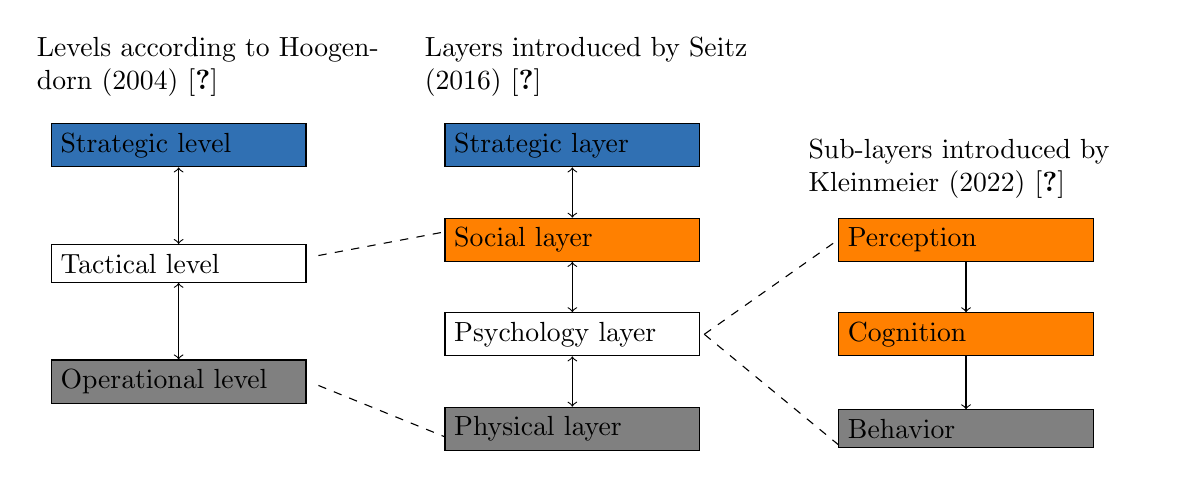
\begin{tikzpicture}[scale=1, transform shape]
\node[text width={4.5cm},anchor=west] at (-5.3, 1) {Levels according to Hoogendorn (2004)~\cite{hoogendoorn-2004-cdyn}};
 \node[fill=blue,anchor=west,rectangle,draw, text width=3cm] (strategie) at (-5,0) {Strategic level};
  \node[rectangle,draw,anchor=west,text width=3cm] (taktik) at (-5,-1.5) {Tactical level};
    \node[fill=gray,rectangle,draw,anchor=west,text width=3cm] (operational) at (-5,-3) {Operational level};
       \draw[<->](strategie) -- (taktik) ;
         \draw[<->](taktik) -- (operational) ;
         
            \draw[dashed] (-1.6,-1.4) -- (0,-1.1);
          \draw[dashed] (-1.6,-3.05) -- (0,-3.7);
                           
  \node[text width={4.5cm}] at (2, 1) {Layers introduced by Seitz (2016)~\cite{seitz-2016-cdyn} };
   \node[fill=blue,anchor=west,rectangle,draw,text width=3cm] (ip) at (0,0) {Strategic layer};
 \node[fill=orange,anchor=west,rectangle,draw,text width=3cm] (ic) at (0,-1.2) {Social layer};
  \node[rectangle,draw,anchor=west,text width=3cm] (b) at (0,-2.4) {Psychology layer};
    \node[fill=gray,rectangle,draw,anchor=west,text width=3cm] (bb) at (0,-3.6) {Physical layer};
 
 \draw[<->](ic) -- (ip) ;
         \draw[<->](ic) -- (b) ;
                  \draw[<->](b) -- (bb) ;

      
      \node[text width={4.5cm},anchor=west] at (4.5, -0.3) {Sub-layers introduced by Kleinmeier (2022)~\cite{kleinmeier-2021-cdyn} };
       \node[fill=orange,rectangle,draw,anchor=west,text width=3cm] (per) at (5,-1.2) {Perception}; 
 
      \node[fill=orange,rectangle,draw,anchor=west,text width=3cm] (cog) at (5,-2.4) {Cognition};
     \node[fill=gray,rectangle,draw,anchor=west,text width=3cm] (bah) at (5,-3.6) {Behavior};
     
              \draw[->](per) -- (cog) ;
                  \draw[->](cog) -- (bah) ;
     
     \draw[dashed] (3.3,-2.4) -- (5,-1.2);
          \draw[dashed] (3.3,-2.4) -- (5,-3.8);

        
\end{tikzpicture}
\caption[The hierarchical modeling approach for crowd behavior]{Hierarchical modeling approaches for crowd behavior. The hierarchic model approach introduced by Hoogendoorn~\cite{hoogendoorn-2004-cdyn} has been refined by Seitz~\cite{seitz-2016-cdyn} and Kleinmeier~\cite{kleinmeier-2021-cdyn}. The refinements allow to model collective, social and psychological behavior. }
\label{fig:hoogendoorn-hierarchisches-modell}
\end{figure}




\begin{figure}[hbt!]
\centering
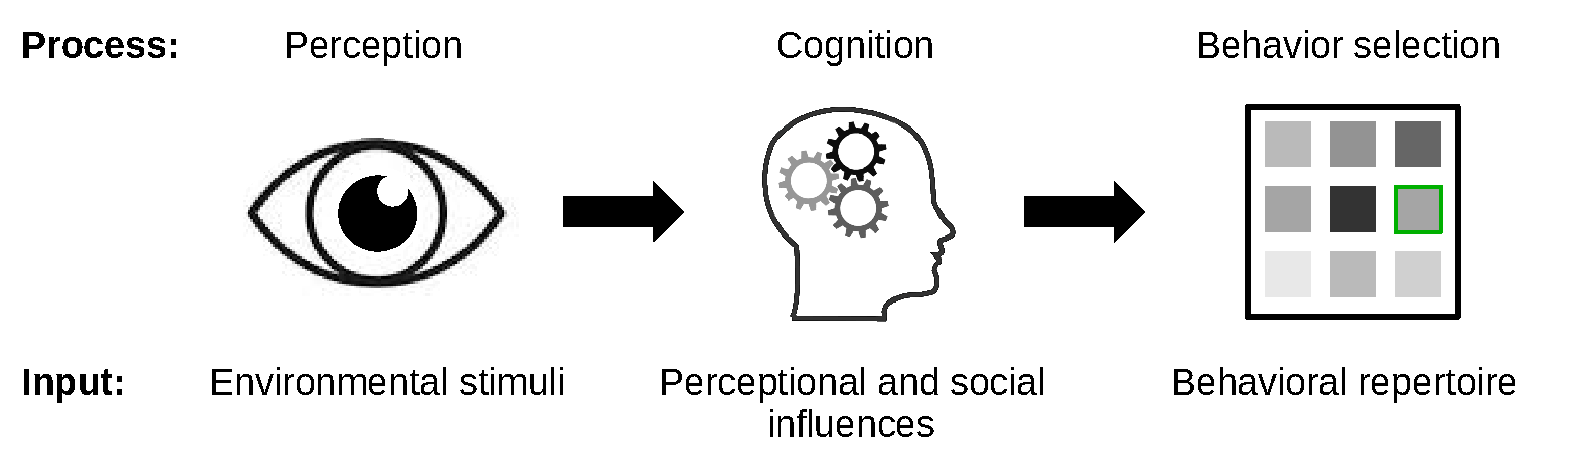
\includegraphics[width=1\textwidth]{../figures/state-of-the-art/crowds/perceptioncognigion.pdf} 
\caption[]{Modeling perception, cognition, and behavior selection.  At the perception layer, the most important stimulus is selected. At the cognition layer, a self-category is selected based on the most important stimulus and environmental conditions. From the self-category, a behavior is selected at the locomotion layer. Own graphics inspired by~\cite[p.89]{kleinmeier-2021-cdyn}.}
\label{fig:perceptioncognition}
\end{figure}




\FloatBarrier




\subsection{Modeling locomotion at the operational layer}

The movement behavior of a crowd is modeled at the operational level. The main inputs of a  locomotion model are a discretized topography with specified start and destination areas, and the crowd size. 

The granularity of the simulation output depends on the type of simulation model. Models can be divided into microscopic, mesoscopic, and macroscopic models~\cite{adrian-2019-cdyn}. Macroscopic models describe the flows of people as a continuum using macroscopic equations. This model group provides macroscopic output variables such as flows and densities. In a microscopic model, each pedestrian is modeled individually as so-called agent. Models from this category provide agent-specific output data, such as trajectories or individual waiting times. 
Mesoscopic models combine microscopic and macroscopic properties. Many of them are multiscale models~\cite{borrmann-2012-cdyn}:
Microscopic models are used in parts of the topography where detailed pedestrians locomotion is needed. Macroscopic models provide pedestrian flows in between these areas. 
Neither macroscopic nor mesoscopic models can capture psychological behavior in detail~\cite{kleinmeier-2021-cdyn}. In a crowd guidance system it is essential to model peoples' responses to route recommendations. Therefore, microscopic models are required. 

Several microscopic locomotion models have been developed in the last decades.
So-called \textit{cellular automatons}~\cite{gipps-1985-cdyn} are zero-order models that consider only the current state (`zero order of the derivative') in the propagation of the movement. The topography is discretized as a grid where each cell is either empty or occupied by a single agent. If a target cell is free and not a target of another agent, a move is executed. If multiple agents share the same target, the agent that has the higher probability is assigned to the cell. The so-called floor field modifies the probabilities to ensure that moves towards the target are preferred~\cite{kirik-2007-cdyn,schadschneider-2001-cdyn}.  

The \textit{Optimal Steps Model}~\cite{seitz-2012-cdyn} is a zero order model that is continuous in space and time. It was validated in several works~\cite{seitz-2016c-cdyn,seer-2015-cs,seitz-2012-cdyn,sivers-2016b-cdyn}. The basic idea is that agents try to improve a utility with every step~\cite{seitz-2012-cdyn}. The utility of each position in space is coded in a scalar function, also called floorfield. The utility, or potential, depends on the geodesic distance to the target and the proximity to other agents, see Fig.~\ref{fig:floorfield}. Utility increases when approaching targets and decreases when getting too close to obstacles and other agents. Physically spoken, agents, when moving, are attracted by targets and repulsed by obstacles and other agents. A dynamic floorfield can be used to model long- and medium-range interactions~\cite{koster-2014b-cdyn}. Sivers et al.~\cite{sivers-2015-cdyn} modified the potential functions based on Hall's theory of interpersonal distances. 





\begin{figure}[hbt!]
\centering
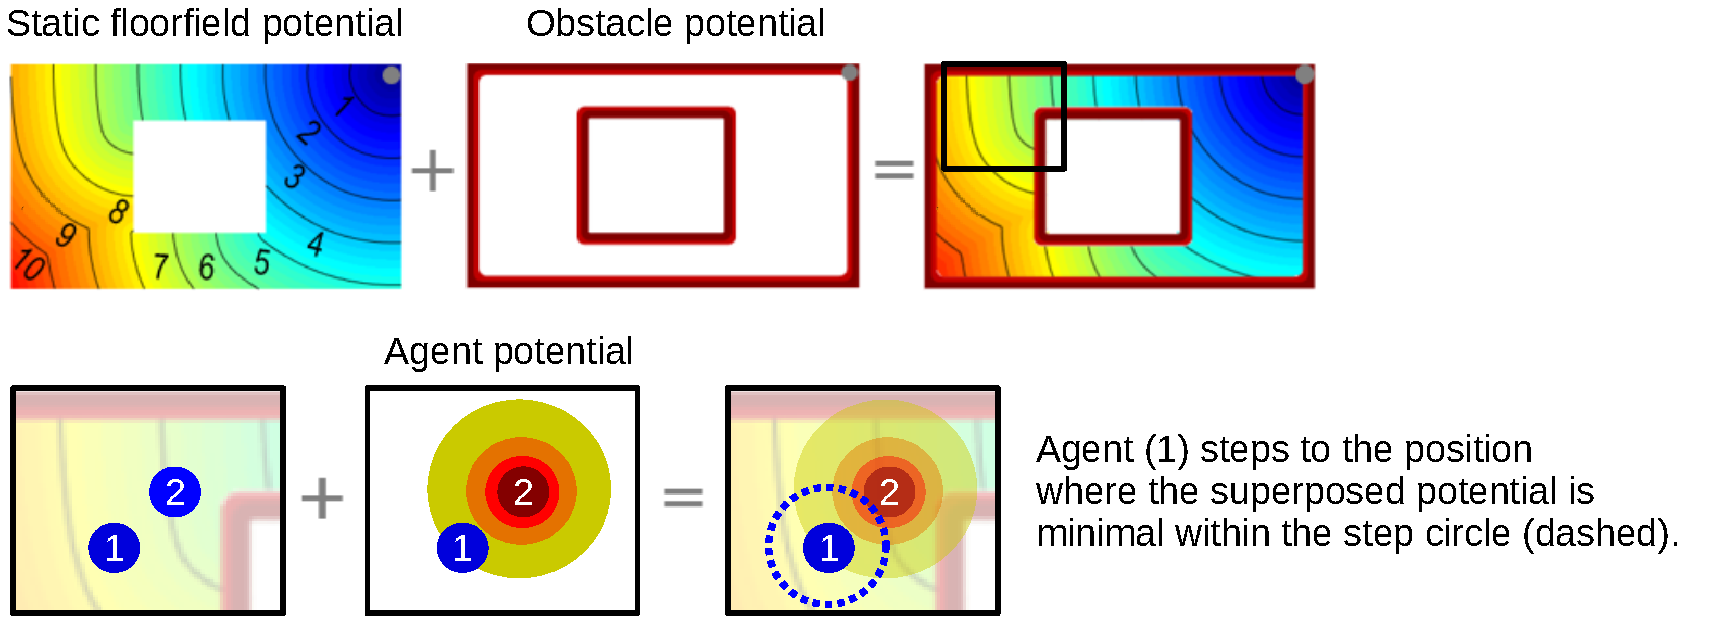
\includegraphics[width=1\textwidth]{../figures/state-of-the-art/crowds/optimalstepsmodel.pdf} 
\caption[Idea of the Optimal Steps Model]{Basic idea of the Optimal Steps Model~\cite{seitz-2012-cdyn}. Agents use the shortest path to a target (floorfield potential) while skirting obstacles (obstacle potential) and other agents (agent potential). The potentials are superposed. 
For each step, the optimal position needs to be found, that is, where the potential has a minumum within a step circle. }
\label{fig:floorfield}
\end{figure}



%
So-called \textit{Velocity-based Models} are first-order models that consider agents' position and speed (first derivative). In contrast to the cellular automaton, this model type is continuous in space.
Velocity-based models are either based on the concept of `optimal velocities' or the concept of `velocity obstacles'. In the `optimal velocities' approach, agents' velocity is adjusted using an optimal velocity function that depends on the minimum spacing in front~\cite{tordeux-2014-cdyn}. In the `velocity obstacles' approach, the orientation and the speeds are varied to find a configuration of agents where they do not collide~\cite{karamouzas-2009-cdyn}. 

So-called \textit{Force Models} are second-order models that employ accelerations (second spatial derivative) and force terms to model repulsion between agents and attraction to target. The most popular force model is the \textit{Social Force Model}~\cite{hirai-1975-cdyn,helbing-1995-cdyn} for which numerous extensions exist, see e.g.~\cite{chen-2018-cdyn}. Social Force Models are widely used in the pedestrian community despite numerical instabilities that can lead to oscillations~\cite{koster-2013-cdyn}.

Hybrid models combine the advantages of velocity-based and force-based models. This modeling approach includes the \textit{Gradient Navigation Model}~\cite{dietrich-2014-cdyn} where velocity and acceleration are considered in a decoupled manner: The position of the next step only depends on velocity-based quantities, but the magnitude of the velocity vector depends on an acceleration term.

So-called \textit{Decision-based or Decision Models} form another model category. These use simple rules for locomotion, such as `slow down', `keep a certain speed', or `accelerate' \cite{antonini-2006-cdyn}. One of them is the \textit{Behavioral Heuristics Model}~\cite{seitz-2016c-cdyn} that has four rules: (1) perform a step towards the target if the position is free. (2) If occupied try to evade tangentially. (3) If the tangential position is occupied perform a side step. (4) If the side is occupied wait.



Which locomotion model is most suitable for an applications depends how much computational effort one is willing to invest and on the required accuracy. Space-continuous models, such as force models or optimal steps models, produce more realistic trajectories than models with spatial discretization, such as the cellular automaton. However, such sophisticated models are computationally expensive: In the Optimal Steps Model an optimization problem needs to be solved for each step. The social force model requires solving a system of differential equations. If the scenario is large and low accuracy is acceptable, space discrete models, such as the cellular automaton, are still in use. Again, there is no model that fits all needs.












\subsection{Modeling route choice at the tactical layer}
Different types of models can be found at the tactical level: models for queuing behavior (see, e.g.,~\cite{kim-2013-cdyn}), models for avoiding crowds~(see, e.g.,~\cite{zoennchen-2013-cdyn}) , and small group models~(see, e.g.,~\cite{seitz-2011-cdyn}). 
Also route choice behavior is modeled at the tactical layer for which one can differentiate two model types, see~Fig.~\ref{fig:differencelinkchoiceroutechoice}.




Link choice models, or traffic assignment models, are used in traffic engineering to model the flow distribution at junctions~\cite{boyce-2021-cdynff}. They model the decision of the entire population depending on the current location in the traffic network. The input of such a model is the network topology and an origin-destination matrix. The output of the model is various route assignments for each origin-destination pair. The assignments are determined by optimizing the route assignments so that the average travel time~\cite{wardrop-1952-cdyn} or an alternative objective becomes minimum. 



\begin{figure}[hbt!]
\centering
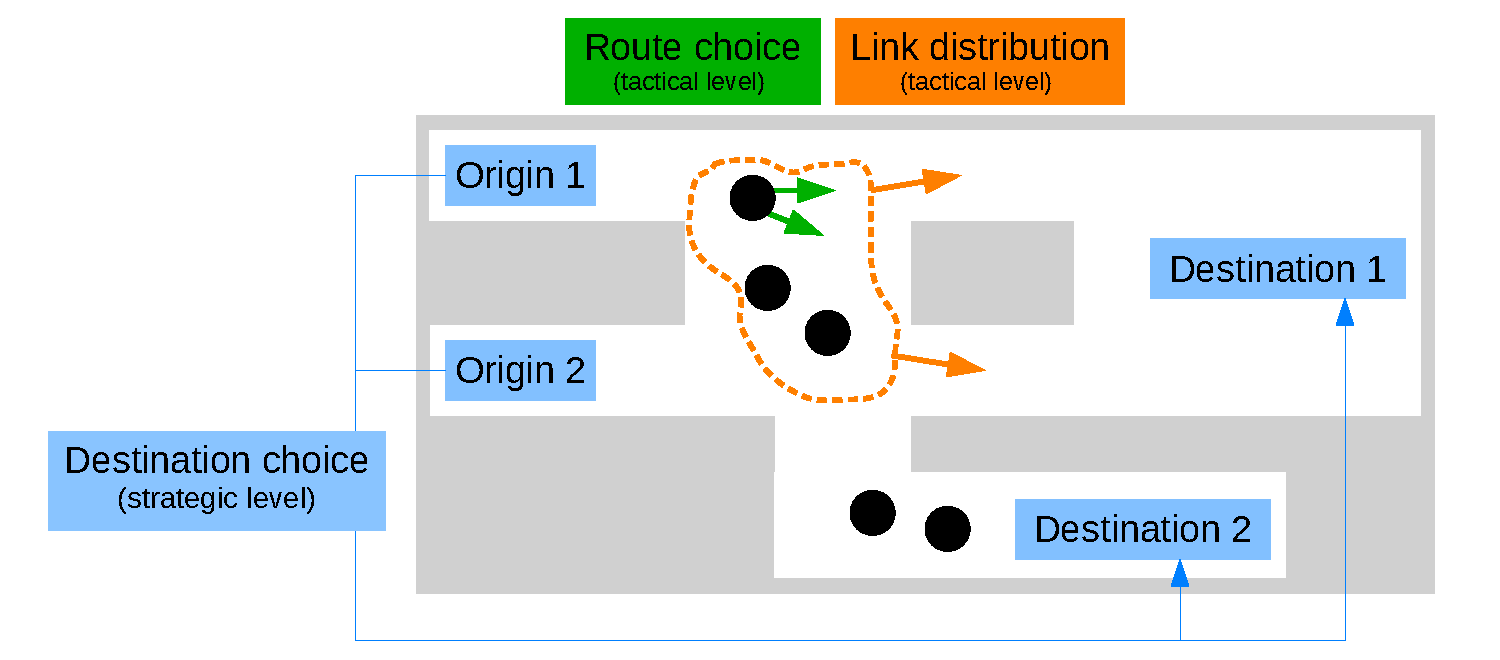
\includegraphics[width=11cm]{../figures/state-of-the-art/crowds/abgrenzung.pdf} 
\caption[Zusammenhang zwischen Modellen des strategischen und taktischen Layers]{Relationship between strategic and tactical layer models.
Route choice models capture individual route choice, while link choice models simulate the route distribution of a population. So-called destination~\cite{danalet-2015-cdyn} and location choice models~\cite{beaulieu-2019-cdyn} belong to the strategic layer.
}
\label{fig:differencelinkchoiceroutechoice}
\end{figure}

Route choice models reflect the decision-making process of an individual. Therefore, they belong to the cognition layer of Kleinmeier's psychology layer~\cite{kleinmeier-2021-cdyn}.
Numerous experiments have been conducted to identify factors or stimuli that affect the route choice, see e.g. \cite{palma-2012-cdyn,crociani-2016b-cdyn,kinateder-2018-cdyn}. 
Many route choice models are multi-logit models that make a route decision based on environmental and exogenous factors~\cite{lopez-2021-cdyn}. 
Shi et al.~\cite{shi-2023-cdyn} propose a conditional multinomial logit model to model the route choice behavior of metro passengers. Daamen~\cite{daamen-2004-cdyn} proposes a logit model that models route choice with the factors of walking and waiting times, route lengths, and walking comfort.
Xu et al.~\cite{xu-2014-cdyn} suggest a model that considers the distance to the exits and their attractiveness. 
Ramos et al.~\cite{ramos-2020-cdyn} use the travel time as a factor in their logit model. 
Tong et al.~\cite{tong-2021-cdyn} extend a logit model proposed by Arganda et al.~\cite{arganda-2012-cdyn} by adding a factor that has the effect that people become "less sensitive to environmental information the more decisions they have to make". In a second study, Tong et al.~\cite{tong-2021b-cdyn} propose to add another factor that models the so-called ‘route commitment effect’, that is,  "the more pedestrians invest into a planned route by walking along it, the more likely they are to adhere to this route even when encountering congestion". 
Other logit models consider stairs~\cite{aleksandrov-2018-cdyn}, visibility conditions~\cite{lovreglio-2016-cdyn,haghani-2018b-cdyn}, the tendency to stick to a route~\cite{haghani-2019c-cdyn}, or the effect of instructions from human guides~\cite{nishida-2023-cdyn}. Apart from route choice models, machine learning has been  proposed to emulate route choice behavior, see e.g.~\cite{zhao-2023-cdyn}.


Few approaches try to model people's compliance to instructions:
Lopez~\cite{lopez-2021-cdyn} split agents into two groups. For non-compliant agents, they use a route choice model. Compliant agents follow the instruction, ignoring other factors.
Haghani et al.~\cite{haghani-2019c-cdyn} use another approach: They implicitly model compliance by introducing a factor called ‘inertia’ to a logit model that biases the decision.




As one can see there are several suggestions to model route choice behavior. All of the proposed models were derived for different factors and scenarios. 
Consequently, the models cannot be simply transferred to arbitrary scenarios. Moreover, there is no approach that models the compliance with route recommendations provided by a mobile application. Therefore, a new modeling approach is needed.




\subsection{Modeling of communication and psychological factors}
How people respond to information depends on how information is communicated, see e.g.~\cite{carter-2015-life}. There are different approaches to model communication aspects. 
Templeton et al.~\cite{templeton-2023-cdyn} distinguishes four principle modeling strategies:

\begin{itemize}
\item Field of influence: Agents have a bounded field of influence around them, which transmits information to other agents. See e.g. \cite{bernardini-2014-cdyn}.
\item Network-based: Agents share information with others within their social network. See e.g. \cite{yang-2019-cdyn}.
\item Information trails: Agents disseminate information via trails in the environment as they move. See e.g.~\cite{zheng-2019-cdyn}.
\item External information: Agents in particular areas become informed by an external source. See e.g. \cite{rigos-2019-cdyn}.
\end{itemize} 

Some other approaches aim to model the effect of the emotional state of an individual. Pelechano et al.~\cite{pelechano-2005-life} propose a model in which the decision-making process depends on the emotional state affected by stress and physiological factors. Bosse et al.~\cite{bosse-2013-life} model the effect of beliefs, desires, and intentions. Kielar~\cite{kielar-2017-cdyn} takes  memory and individual preferences into account. %Pan~\cite{pan-2006-cdyn} 
Wijermans~\cite{wijermans-2011-cdyn} considers the effect of the physiological constitution.
 
Some approaches focus on modeling social identities (Section~\ref{sec:crowdbah}). In her dissertation, Sivers~\cite{sivers-2016c-cdyn} modeled the effect of social identities on helping behavior. Kleinmeier~\cite{kleinmeier-2021-cdyn} investigated how cooperative behavior between group members can be modeled using self-categories.

The brief overview shows that there are indeed approaches for modeling psychological changes and the communication in a crowd. However, it is unclear how one can model the effect of route recommendations that are communicated via mobile applications in combination with social identities in a crowd guidance system. 




\subsection{Simulation frameworks}
\label{sec:crowdssimframeworks}

Several open-source simulation frameworks are available to simulate crowd behavior, see Tab.~\ref{tab:overviewcrowdsimulators}. Some of them are no longer maintained. Most of them operate at the operational layer, that is, providing locomotion simulation. The only simulator providing a psychology layer is the \textit{Vadere} simulation framework~\cite{kleinmeier-2021-cdyn}.



\begin{table}[hbt!]
\begin{footnotesize}

\begin{tabular}{p{2.7cm}p{3.3cm}p{2.5cm}p{1.8cm}p{1.8cm}}
\hline
\textbf{License} & \textbf{ Simulator} & \textbf{Language} & Reference & Maintained \\
\hline
LGPL & JuPedSim & C++,Python  &\cite{chraibi-2016-cs}\\
LGPL & Vadere & Java & \cite{kleinmeier-2019-cdyn}\\
GPLv3 & GAMA & Java & \cite{taillandier-2017-cdyn}\\
MIT & Agents.jl & Julia & \cite{datseris-2022-cdyn}\\
LGPL v3 & jCrowdSimulator & Java & \cite{meinert-2019-cdyn}  \\
GNU GPL & Cromosim &  Python & \cite{maury-2019-cdyn}  \\
Apache 2.0  & Mesa & Python & \cite{masad-2015-cdyn}\\
\hline
GPLv3 & PedSim & JavaScript & \cite{gloor-2005-cdyn}  & no \\
Apache 2.0 &  Menge & C++ & \cite{curtis-2016-cdyn} & no \\
- & FDS+Evac  & Fortran & \cite{korhonen-2007-cdyn} & no \\
- & MomenTUMv2 & Java & \cite{kielar-2016b-cdyn} &  no \\
 \hline
%Commercial & AnyLogic & Java  \\
%& crowd:it & Java\\
%& PD Pedestrian Dynamics & 4DScript \\
%& MassMotion  & Python,Java,C++,C\# \\
%& Crowd.lab & C++,JavaScript \\
%& SimWalk & C++ \\
%& PTV Vissim & Unknown \\
%& UCrowds & C++ &  \\

\end{tabular}
\end{footnotesize}
\caption[]{Overview on open-source software for crowd simulations. The list is based on Richard's software review~\cite{richards-2020-cdyn}. I consider simulators as no longer maintained when the last commit was before Dec 2022 (checked: 18 Jan 2024). }
\label{tab:overviewcrowdsimulators}
\end{table}


\section{Modeling mobile networks and direct communication}

\label{sec:modelcom}


This section belongs, like the previous section, to the second part of the state of the art. I present the state-of-the-art of modeling and simulating direct communication in mobile networks. First, standards on mobile communication and their respective protocol stacks are introduced. Then, an overview of channel modeling is given. Finally, I present state-of-the-art system level simulators. I assume that the reader is familiar with the ISO/OSI reference model and the basic principles of radio wave propagation such as \enquote{free-space (or line-of-sight) propagation, transmission (and absorption), specular reflection, diffraction, and diffusion (also known as diffuse scattering) [...]}~\cite{rappaport-2001-com}. If not, I recommend to~\cite{rappaport-2001-com}.



\subsection{Overview of mobile standards enabling direct communication}

For enabling device-to-device (D2D) communication, two main technologies have emerged: dedicated short-range communication based on the IEEE 802.11p standard~\cite{802.11p-2010-com} and cellular vehicle-to-everything (C-V2X) communication based on several releases of the 3rd Generation Partnership Project (3GPP), see Fig.~\ref{fig:protocollstack}.
% .There are also approaches to enable direct communication via 5G mmWave.


\begin{figure}[hbt!]
\centering
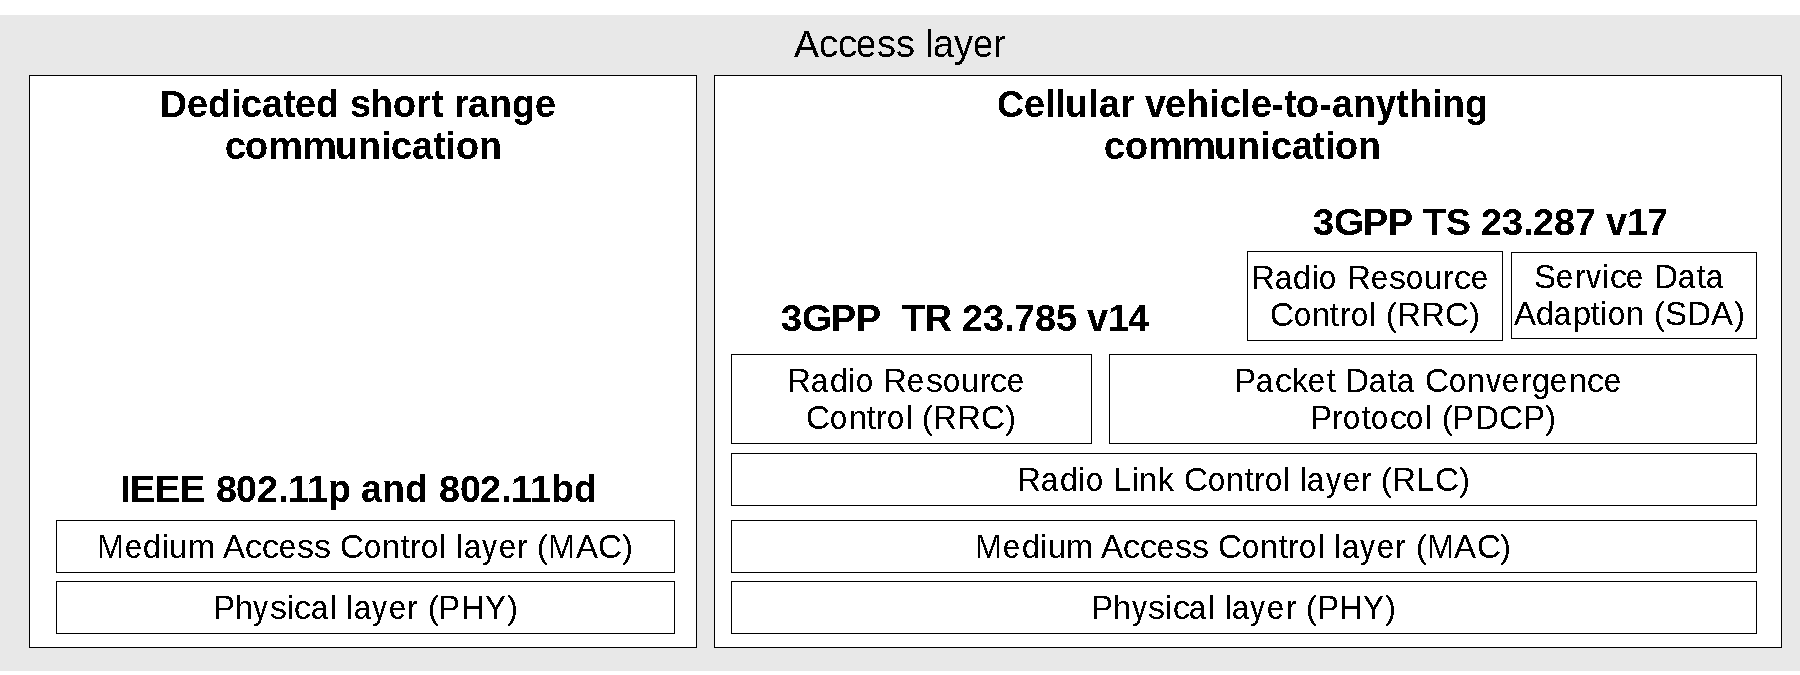
\includegraphics[width=\textwidth]{../figures/state-of-the-art/mobilecommunication/protocollstacks.pdf} 
\caption{Protocol stack reference model for direct communication. Standards for direct communication specify the lower layers of the protocol stack.  Own graphics, inspired by~\cite[p.89]{chen-2023-com}. }
\label{fig:protocollstack}
\end{figure}



\subsubsection{Dedicated Short Range Communication}

The \textit{IEEE 802.11p} standard~\cite{802.11p-2010-com} was the first mobile standard enabling Device-to-Device~(D2D) communication. It specifies Dedicated Short Range Communication (DSRC) on the physical layer and on the medium access control (MAC) layer. At the physical layer, the Orthogonal Frequency Division Multiplexing (OFDM) is specified for the modulating of data on multiple carrier frequencies.
At the medium access control (MAC) layer, the standard specifies the Enhanced Distributed Channel Access (EDCA) method that employs carrier sense multiple access with collision avoidance (CSMA/CA): Before a packet is sent, the network node checks whether the transmission channel is free. If the channel is busy, the node waits for a randomly defined period of time and then checks again.
Therefore, participants access the channel in a self-organized, decentralized way. However, this requires that devices recognize the channel occupation correctly and do not start accessing the channel simultaneously. Therefore, the performance depends on the density of participants. The more participants, the more likely are collisions and interference that lead to packet loss~\cite{shrestha-2020-com}. It cannot be guaranteed that packets arrive within a certain time~\cite{shrestha-2020-com}.

As the 802.11p standard only applies to the physical and medium access control layer, the standard is combined with other standards to enable Dedicated Short Range Communication. In the context of Intelligent Traffic Systems (ITS), there are the IEEE 1609 standard~\cite{ieee-2016-IEEEStd1609.4-com} (USA), the CEN/ETSI EN302 663 standard~\cite{etsi-2019-EN302663-com} (Europe) and the ARIB STD-T109 standard~\cite{its-2012-T109-com} (Japan). An overview of the country-specific specifications can be found in~\cite{costandoiu-2019-com}.
The transmission is intended to operate in the frequency range 5855\,MHz to 5925\,MHz. 

The \textit{IEEE 802.11bd} standard~\cite{ieee802.11bd-2022-com} is an amendment of the set of 802.11 standards. It was released in 2023, and it is interoperable with the 802.11p technology. The amendment aims to improve throughput, latency, reliability, and range through new specifications for the physical layer and the medium access layer~\cite{yacheur-2020-com}.  Therefore, 802.11bd-based technology is more advanced than \textit{IEEE 802.11p} technology. The bandwidth of the channel is $20\,MHz$ which is twice the bandwidth of the IEEE 802.11p standard. Like the IEEE 802.11p, the amendment specifies the EDCA method for accessing the channel. Due to the larger bandwidth and adjustments regarding the error correction scheme, more packets can be transmitted~\cite{yacheur-2020-com}. 
Although the 802.11bd amendment has improved network performance compared to the 802.11p standard, 802.11bd-based technology can often not outperform Cellular Vehicle-to-everything communication, as demonstrated in~\cite{anwar-2019-com}.


\subsubsection{Cellular Vehicle-to-everything communication}
Cellular Vehicle-to-everything communication (C-V2X) has been developed by the Third Generation Partnership Project (3GPP), see Fig.~\ref{fig:overviewofreleases3gpp}. 


\begin{figure}[hbt!]
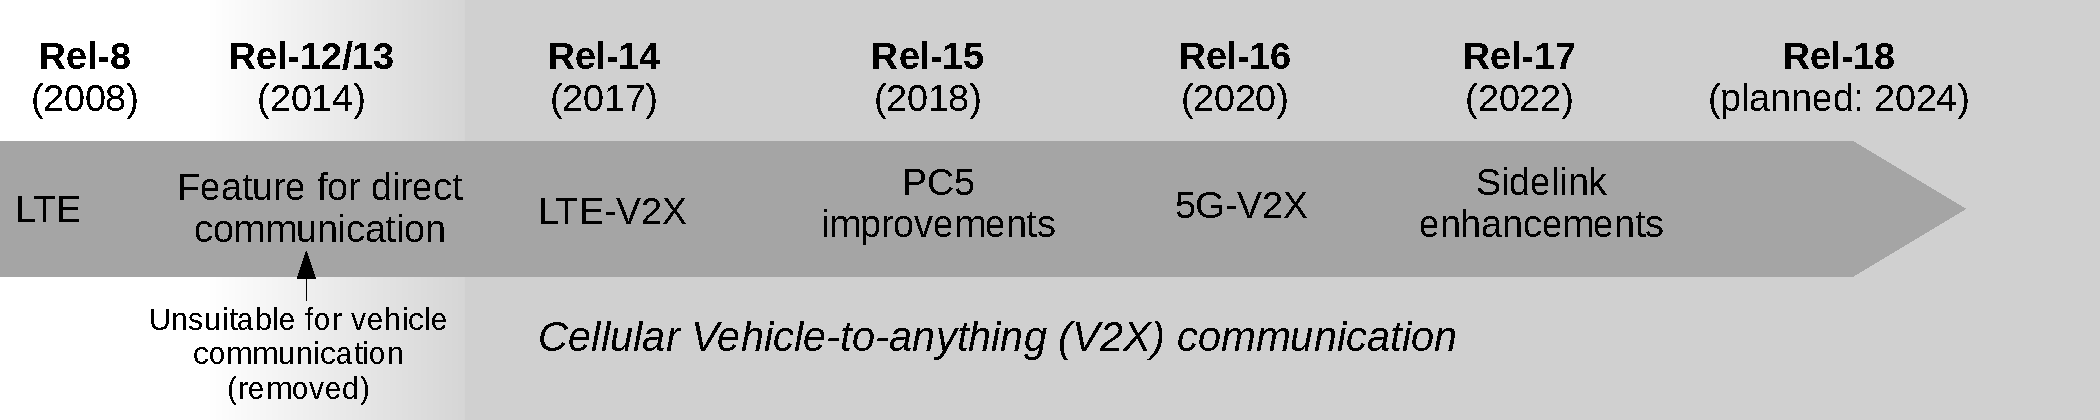
\includegraphics[width=\textwidth]{../figures/state-of-the-art/mobilecommunication/release3gpp.pdf} 
\caption{Standards of the 3rd Generation Partnership Project (3GPP) for Cellular Vehicle-to-everything communication. Own graphics; inspired by~\cite{bazzi-2021-com}.}
\label{fig:overviewofreleases3gpp}
\end{figure}


\textit{LTE V2X}, that is Vehicle-to-everything communication over Long Term Evolution networks, is specified in the technical reports TR 22.885~\cite{3gpp-22.885-2015-com} and TR 36.885~\cite{3gpp-36.885-2016-com} as well as in the technical specifications TS 22.185~\cite{3gpp-22.185-2020-com}, TS 23.285~\cite{3gpp-23.285-2020-com}, TS 36.213~\cite{3gpp-36.213-2020-com}, TS 36.321~\cite{3gpp-36.321-2020-com} released by the 3GPP. Direct communication is specified over the PC5 interface using so-called sidelinks. The sidelink uses the same band for communication as the Dedicated Short Range Communication: $5.9\,\text{GHz}$.
Two communication modes exist: the controlled mode (mode 3) and the autonomous mode (mode 4), see Fig.~\ref{fig:scenariosmodes}. In mode 3, a base station allocates resources. In this mode it is not specified whether dynamic or semi-persistent scheduling is employed~\cite{bazzi-2021-com}. 
For the autonomous mode a semi-persistent scheduling procedure is required: each network participant allocates frames and sub-channels at a fixed time interval based on channel occupancy estimates~\cite{bazzi-2021-com}. 



\begin{figure}[hbt!]
\centering
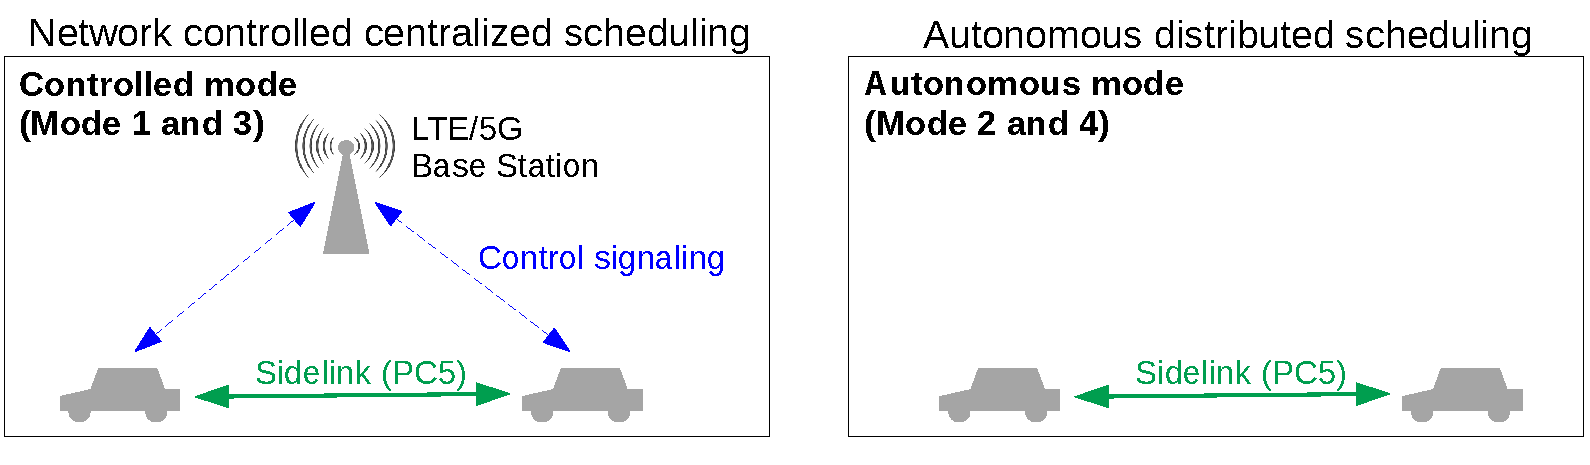
\includegraphics[width=1.0\textwidth]{../figures/state-of-the-art/mobilecommunication/cellularmodes.pdf} 
\caption[Direct communication scenarios in a cellular network]{Modes for cellular vehicle-to-everything communication. Vehicles (or devices) share data directly over the PC5 interface using so-called sidelinks. In mode 1 (5G) and 3 (LTE) the base station allocates resources to reduce the risk of  collision and interference (left). In mode 2 (5G) and 4 (LTE), vehicles schedule packet transmissions autonomously~\cite{bazzi-2021-com}.  }
\label{fig:scenariosmodes}
\end{figure}





\textit{5G V2X} or \textit{NR-V2X}, where NR stands for `New Radio', means communication over sidelinks in networks of the fifth generation (5G). The 5G sidelink is defined by the 3GPP in the documents TR 22.886~\cite{3gpp-22.886-2018-com}, TR 38.885~\cite{3gpp-38.885-2019-com}, TS 23.287~\cite{3gpp-23.287-2020-com}, TS 22.186~\cite{3gpp-22.186-2019-com}, TS 38.213~\cite{3gpp-38.213-2020-com}, TS 38.321~\cite{3gpp-38.321-2020-com} and TS 37.895~\cite{3gpp-37.895-2020-com}. 
5G sidelinks and LTE sidelinks differ in their waveform, the scheduling interval, and the channel coding procedure, see Tab.~\ref{tab:directcom-overview}. As with LTE sidelink communication, one can distinguish a controlled (mode 1) and autonomous mode (mode 2). 
Importantly, the 5G sidelink operates at two frequency bands: $0.41\,\text{GHz}$-$ 7.125\,\text{GHz}$ and $24.25\,\text{GHz}$-$52.6\,\text{GHz}$. For the latter, the wavelength is at the scale of a millimeter, which is why it is referred to as 5G millimeter waves (mmWaves). 






\subsubsection{Overview on technologies and interoperability}
An overview of specifications and technologies can be found in Tab.~\ref{tab:directcom-overview}.
Importantly, dedicated short range communication technologies and cellular technologies are not interoperable~\cite{molina-2020-com}. Even in a `hybrid system', the technologies operate simultaneously but independently~\cite{shrestha-2020-com}.
The 802.11bd standard~\cite{ieee802.11bd-2022-com} is compatible with its predecessor IEEE 802.11p. The LTE sidelink and the NR sidelink are basically not interoperable, but they can co-exist~\cite{bazzi-2021-com}. 



\begin{table}[hbt!]
\begin{footnotesize}
\begin{tabular}{|p{2.4cm}|p{2.5cm}|p{2.5cm}|p{2.5cm}|p{2.5cm}|}
\hline 
\textbf{Standard} & \textbf{802.11p} &  \textbf{802.11bd} & \textbf{LTE V2X} & \textbf{5G/NR V2X} \\ 
\hline 
Technology & WLAN & WLAN & 4G/LTE & 5G \\ 
\hline 
First release & 2012 & 2023 & 2017/18 (3GPP Rel-14/15) & 2020 (3GPP Rel-16)  \\ \hline
Wave form & OFDM & OFDM & SC-FDMA & OFDM \\ 
\hline 
Ressource allocation & decentral & decentral  & central (Sidelink mode 3), decentral (Sidelink mode 4) &  central (Sidelink mode 1), decentral (Sidelink mode 2) \\ \hline

Modes & Broadcast & Broadcast, groupcast & Broadcast & Broadcast,
groupcast, unicast
\\ \hline 
Range & short range &  short range & extended range
 & extended range \\ 
\hline 
Scheduling interval &None& None & One sub-frame & Slot, mini-slot or multi-slot \\
\hline
Channel coding & Binary Convolutional Coding (BCC)  & LDPC & Data: Turbo, 
Control: Convolution & Data: LDPC, Control: Polar 
\\ \hline 
Frequency band & 5.9\,GHz & 5.9\,GHz/ 60\,GHz & 5.9\,GHz &  0.41\,GHz-7.125\,GHz, 24.25\,GHz-52.6\,GHz (mmWave) \\ \hline 
Sub-carrier spacing &  156.25\,KHz & 312.5\,KHz, 156.25\,KHz, 78.15\,KHz & 15\,KHz & 15\,KHz, 30\,\,KHz, 60\,KHz, 120\,KHz \\ \hline 
Retransmission & None  & Congestion dependent & Blind & HARQ-based \\ 
%Cyclic Prefix (CP) & 1.6 us & 1.6 us and 3.2 us  & & \\
%High density support & Packet loss at high density & • & No packet loss guaranteed
%at high density & • \\ 
%Security and Privacy
% & Yes (based on IEEE WAVE \&
%ETSI ITS security services) & Yes (based on IEEE WAVE \&
%ETSI ITS security services) & Yes (based on IEEE WAVE \&
%ETSI ITS security services) & Yes (based on IEEE WAVE \&
%ETSI ITS security services) \\  
%\hline 
%Latency & Low  V2V
%communications & • & Round trip latency less than 1ms & • \\ \hline 
\hline 
\end{tabular} 
\end{footnotesize}
\caption[Overview of standards for direct communication]{Overview of standards for direct communication. The IEEE technologies are not interoperable with cellular technologies. The table is based on the data from~\cite{shrestha-2020-com,bazzi-2021-com,molina-2020-com}.}
\label{tab:directcom-overview}
\end{table}














\subsection{Modeling wireless propagation channels}
For a mobile network simulation, it is essential to model the propagation channel.
\enquote{A wireless propagation channel is the medium linking the transmitter and the receiver. Its properties determine the information-theoretic capacity, i.e., the ultimate performance limit of wireless communications, and also determine how specific wireless systems behave. It is thus essential that we know and understand the wireless propagation channel and apply this knowledge to system design.}~\cite[p.45]{molisch-2011-com}. 

\newpage

Molisch~\cite[p.125ff]{molisch-2011-com} distinguishes three basic modeling approaches:
\begin{itemize}
\item `Deterministic' channel modeling: solve Maxwell's equation to compute channel characteristics. Since solving the integrals or differential equations is time-consuming, ray-based methods are used in practice. This approach is often applied in network planning and system deployment.
\item `Stochastic' channel modeling: use models to estimate statistical properties of the channel characteristics. This approach is often applied when designing and comparing systems.
\item Use of measurement data: use empirical data to describe the channel characteristics. The execution of a model is not necessary. This approach is often applied when measurement data is available for a specific scenario.
\end{itemize}

Channel models can be classified according to their temporal and spatial resolution~\cite[p.70]{rappaport-2001-com}: so-called large-scale propagation models predict the average signal strength over the distance and are typically used to estimate the coverage. Small-scale or fading models model the signal strength at a fine local (wavelengths) and temporal (seconds) scale~\cite[p.70]{rappaport-2001-com}.


Four channel model categories are differentiated~\cite{molisch-2011-com}, see Fig.~\ref{fig:pathlossmodelsoverview}. Narrowband models describe the signal attenuation. Wideband models focus on the dispersion of the signal. Directional models capture directional properties of signal components, which is why these models are suitable for the simulation of multi-antenna systems~\cite[p.445]{molisch-2011-com}. `Deterministic' models are based on Maxwell's theory of wave propagation.

\begin{figure}[hbt!]
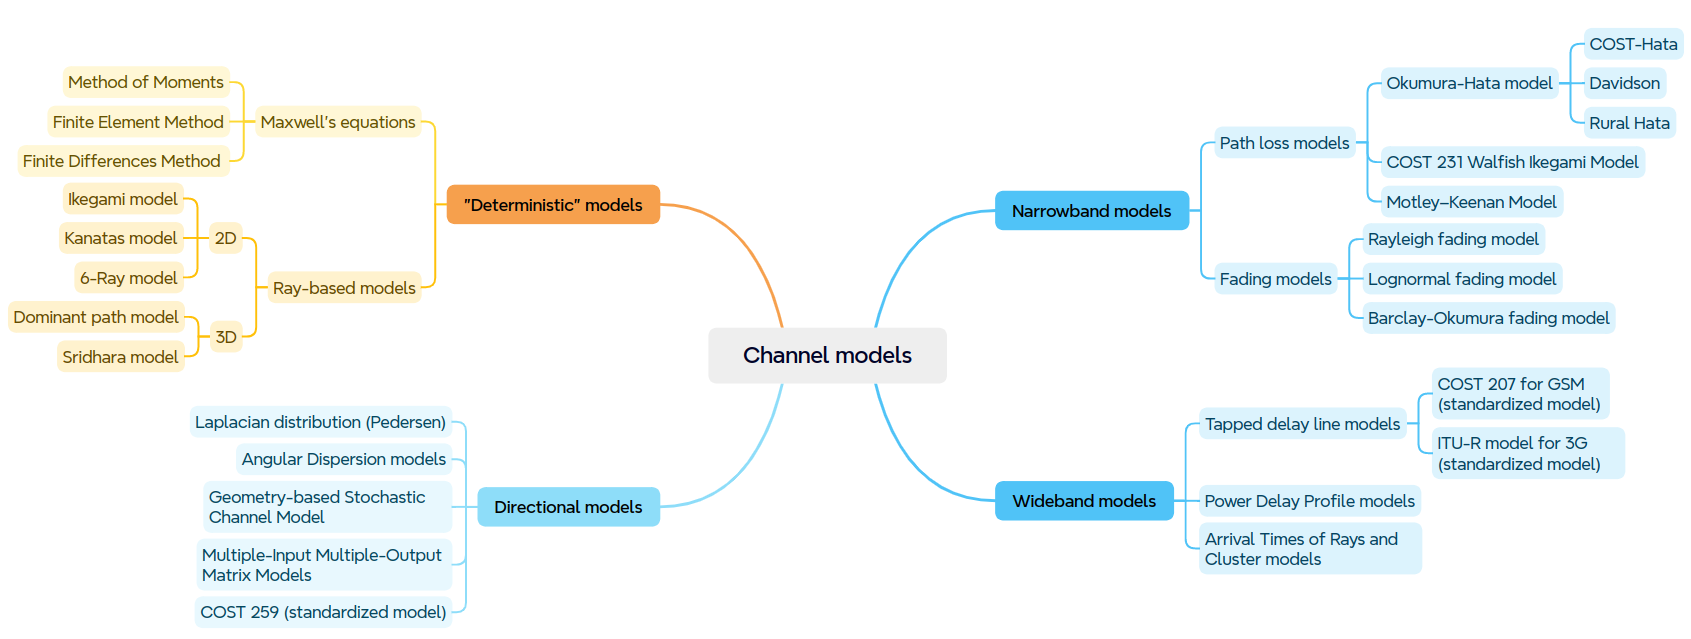
\includegraphics[width=1.0\textwidth]{../figures/state-of-the-art/mobilecommunication/channelmodelv2.png} 
\caption{Classification of channel models according to Molisch~\cite{molisch-2011-com}. The model examples come from Molisch~\cite{molisch-2011-com} and Phillips et al.\cite{phillips-2013-com}. Own graphic inspired by \cite{molisch-2011-com,phillips-2013-com}.}
\label{fig:pathlossmodelsoverview}
\end{figure}

Apart from that, there are different approaches how a channel can be represented as model. Phillips et al.~\cite{phillips-2013-com} distinguishes several categories: (1) Theoretical models are derived analytically from the theory of ideal electromagnetic propagation. An example is the free space path loss model according to Friis~\cite{friis-1946-com} that describes how the power decreases quadratically over the distance between transmitter and receiver. An extension of Friis' model is the Two-Ray Ground Reflection model that considers reflections from the ground~\cite[p.95]{rappaport-2001-com}. 
%
The second category is formed by so-called (2) basic models that are derived from empirical data. 
The Okumura-Hata Model~\cite{okumura-1968-com} describes the path loss depending on the distance between sender and receiver, the frequency, and the height of the base station or mobile station. The model is intended for scenarios with an elevated station, e.g., at a rooftop. Numerous extensions exist, such as the COST Hata Model, which is applicable even for frequencies above $1500\,$MHz~\cite{hata-2023-com}. 


For outdoor scenarios so-called (3) terrain models are used. They are similar to basic models but also consider diffraction. Stochastic fading models (4) add a random variable to capture fading. Models from this category are typically used to design the physical or link layer~\cite{phillips-2013-com}. One of them is the Lognormal Shadowing Model, which can be considered a stochastic version of Friis model with a variable decay parameter. Stochastic fading models, such as the Rayleigh Fading model~\cite{sklar-1997-com}, model small-scale effects. 
Ray-based models (5)  try to capture the effect of wave propagation in the entire space using rays. Supplementary models (6) adjust the results of other models. Many of these models focus on adjusting the signal propagation due to obstacles such as trees or walls, see e.g.~\cite{durgin-1998-com,jong-2004-com,torrico-1998-com}. The so-called ideal obstacle loss model~\cite[p.75]{virdis-2019-com} models the extreme case: If an obstacle is in the line-of-sight, the signal strength is zero. More model examples can be found in~\cite{phillips-2013-com}. 



%\subsection{Overview of standardized channel models}
Standardized channel models are established models that are used by the mobile networks community to develop higher layer protocols and applications.
They are released by standardization institutions such as 3rd Generation Partnership Project  or IEEE, see Tab.~\ref{tab:standardchannelmodels}. The models have been extensively calibrated or validated using empirical data and simulation data, see \cite{erceg-2004-com, winner-2007-com,3gpp2-2003-com,3gpptr36873-2017-com,liu-2012-com,itu-2017-com,tr38901-2018-com,raschkowski-2015-com,peter-2017-com,jaeckel-2019-com} and their references.  I do not want to develop direct communication technologies further, but I want to test their suitability for crowd management applications. Therefore, I employ standardized models for my investigations.
 

\begin{table}[hbt!]
\begin{footnotesize}
\begin{tabular}{p{2.0cm}p{1.2cm}p{6.5cm}p{3.2cm}}
\hline 
{Standard} & {Year} & {Channel model} & {Gremium} \\
\hline
802.11n & 2004 & 802.11n channel model \cite{erceg-2004-com} & IEEE \\
%802.15.3a/4a & 2003/4 & 802.15.3a/4a channel model \cite{molisch-2003-com,molisch-2004-com} & IEEE \\
%802.16 & 2001 & SUI model \cite{erceg-2001-com} & IEEE \\
LTE & 2007 & WINNER model \cite{winner-2007-com} & WINNER project \\
LTE & 2003 & 3D Spatial Channel Model (TR 25.996) \cite{3gpp2-2003-com} & 3GPP \\
LTE & 2017 & 3D Channel Model (TR 36.873) \cite{3gpptr36873-2017-com} & 3GPP \\
LTE & 2012 & COST 2100 model \cite{liu-2012-com} & COST 2100 \\
5G & 2017 & ITU-R channel model \cite{itu-2017-com} & ITU-R \\
5G & 2018 & 3GPP TR 38.901 \cite{tr38901-2018-com} & 3GPP \\
5G & 2015 & METIS \cite{raschkowski-2015-com} & European Commission \\
5G & 2017 & mmMAGIC \cite{peter-2017-com} & Frauenhofer \\
5G & 2019 & QuaDRiGa \cite{jaeckel-2019-com} & Frauenhofer \\
\hline 
\end{tabular} 
\end{footnotesize}
\caption{Examples of standardized channel models. Several models are available for modeling radio channels for different network technologies.  These models are typically used for the development of protocols and applications at higher layers, such as the application layer. }
\label{tab:standardchannelmodels}
\end{table}



\subsection{Simulation frameworks}
\label{sec:mobilenetworkssimulationframeworks}

System-level simulators provide, in contrast to link-level simulators, implementations of the full protocol stack. An overview of simulators can be found in Tab.~\ref{tab:overviewcrowdsimulators}.
Only the two simulation frameworks \textit{OMNeT++}~\cite{varga-2019-com} and \textit{ns-3}~\cite{riley-2010-com} have established themselves as scientific open-source software. The frameworks and their related model libraries provide implementations for standardized channel models including the channel. For example, the 3D channel model TR 36.873~\cite{3gpptr36873-2017-com} is available in the \textit{simu5G}~\cite{3gpptr36873-2017-com} simulator that belongs to the \textit{OMNeT++} ecosystem~\cite{nardini-2020b-com}.


\begin{table}[hbt!]
\begin{tabular}{p{2.7cm}p{3.2cm}p{2.5cm}p{1.8cm}p{1.8cm}}
\hline
{Simulator} & {License} & {Language} & Reference & Maintained \\
\hline
OMNeT++ & Academic public & C++ & \cite{varga-2019-com} \\
ns-3 & GNU GPLv2 & C++, Python & \cite{riley-2010-com} \\ 
GloMoSiM & Academic public & Parsec, Java & \cite{zeng-1998-com} & no \\
LTE-SIM & GPL-3.0 license & C, C++& \cite{piro-2011-com} & no\\
Jist/Swans & CRF & Java & \cite{barr-2004-com} & no\\ \hline
\end{tabular}
\caption[]{Overview of open source software for mobile network simulations. The list is based on Khan's software review~\cite{khan-2012-com}. I consider simulators as no longer maintained when the last commit was before Dec 2022 (checked on 25 Jan 2024). }
\label{tab:overviewcrowdsimulators}
\end{table}

Different studies demonstrate that the mobility behavior of mobile nodes has a major impact on the  mobile network simulation: Wischhof et al.~\cite{wischhof-2022b-com} demonstrated that the results of the mobile networks simulation depend on the accuracy of the locomotion model.
Bai et al.~\cite{bai-2004-com}  found  that path duration in ad hoc networks depends on the accuracy of node movement. They tested different mobility models. Chancay-Garc\'{i}a et al.~\cite{chancay-2018-com} found that information dissemination depends on the degree of motion and message size. 
For this reason, \textit{OMNeT++} and \textit{ns-3} have an interface that allows one to use pre-generated mobility traces in the network simulation. It is also possible to obtain position data online from the SUMO simulator over an interface~\cite{wegener-2008-com}. 

The SUMO simulator~\cite{wegener-2008-com} provides simple pedestrian models where agents move, for example, along lanes like vehicles. These models are not validated against empirical data from pedestrian dynamics research. It cannot be ensured that they produce realistic trajectories. Consequently, safety-critical pedestrian densities cannot be evaluated reliably. I conclude that it is essential to use a validated locomotion model in the investigation of a crowd guidance system. Because several crowd models and simulators are already available (Section~\ref{sec:crowdssimframeworks}), I look at model and simulator coupling in the next section.


%Therefore it is necessary to use validated pedestrian mobility models when investigating the suitability of a mobile communication for the redirection of crowds. 

\FloatBarrier


\section{Model composition and coupling}
\label{sec:simulationframeworks}

In the previous sections (Sections~\ref{sec:modelcrowd}-\ref{sec:modelcom}), I introduced crowd models and mobile network models. These models are separate models that are usually executed independently from each other. For the simulative investigation of a crowd guidance system, these models need to be connected. In this section, I present state-of-the-art approaches how separate models and simulators can be coupled. First, model coupling is discussed for different system types. Next, sequential update procedures are introduced. Then, it is discussed how the data exchange between simulators can be realized. Finally, state-of-the-art simulation frameworks and interfaces are presented.

\subsection{Coupling models and simulators}
With model coupling, two different component models are connected so that they can exchange information with each other.  What a model coupling looks like depends strongly on the structure of the system, see Fig.~\ref{fig:modelcouplingapproaches}. In partitioned multi-physics systems, the model coupling is located at a geometric boundary. Both components share a system state at the boundary. To couple models, the \textit{monolythic approach} or the \textit{partioned approach} can be used. 
\enquote{The monolithic approach, on one hand, uses a single system of equations to describe and solve the coupled problem. On the other hand, partitioned methods use existing single-physics solvers and couple them to a simulation that strives to solve the overall coupled problem}~\cite[p.16]{lindner-2019-cs}.  


\begin{figure}[hbt!]
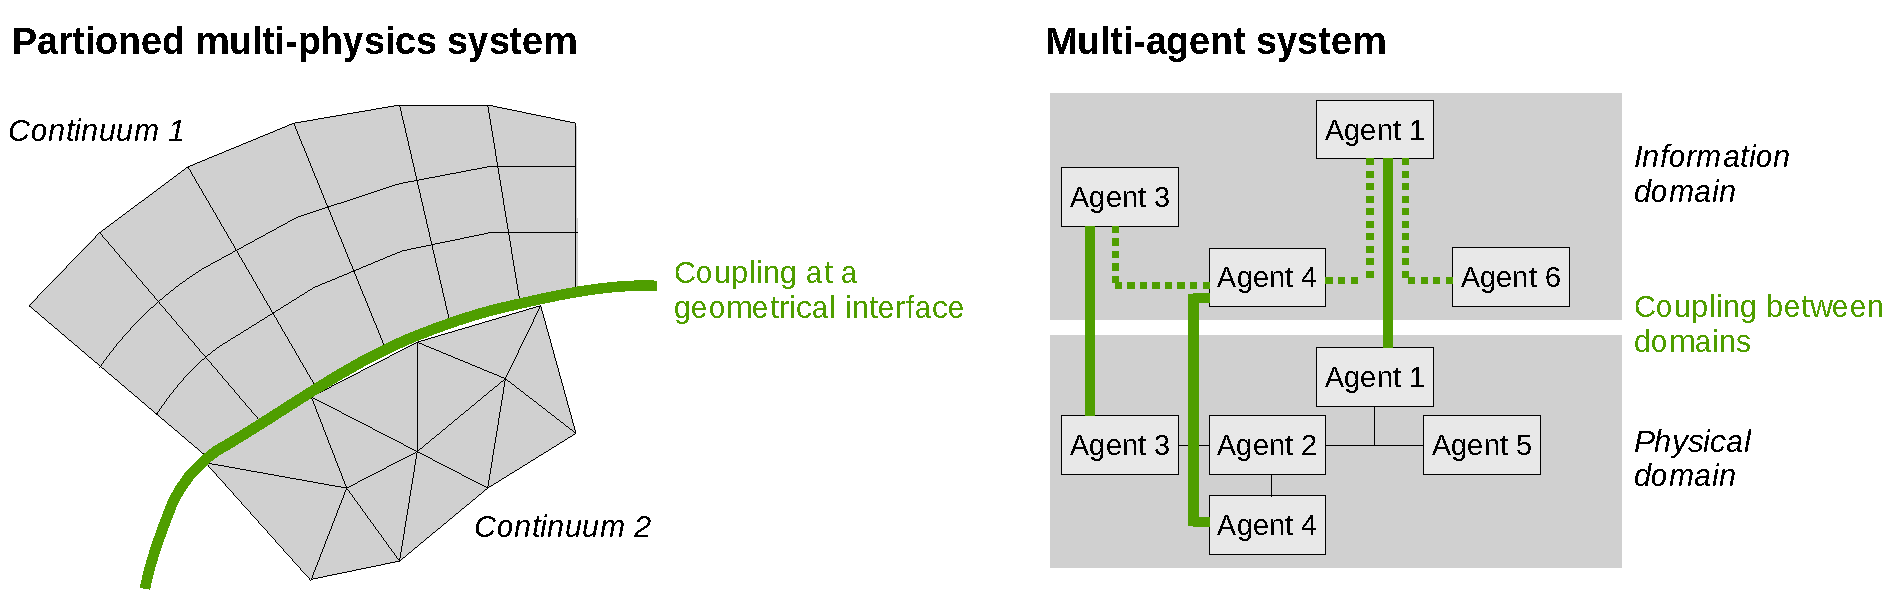
\includegraphics[width=\textwidth]{../figures/state-of-the-art/coupling/modelcouplingapproaches.pdf} 
\caption{Couplings for different system types. In a multi-physics system, interactions occur at a geometric interface (left). An example is an airplane wing: the wing is a mechanical structure that bends through the air that streams along its surface (geometric boundary). In a multi-agent system, the coupling connects the physical and the information domain. One example is a smart   grid, where consumers and producers share information with the goal to improve the electrical supply. The topology of the two domains can differ (compare the two domains on the right). Own graphics; right side inspired by~\cite{schuette-2012-cs}. }
\label{fig:modelcouplingapproaches}
\end{figure}
In a multi-agent system, the model coupling connects the physical domain and the information domain. This type of simulation is sometimes referred to as co-simulation~\cite{schloegl-2015-cs}. The distinction of the two domains comes from the field of smart grid applications in which an electricity grid (physical domain) is controlled with the help of information transmitted via a network (information domain)~\cite{schuette-2012-cs,steinbrink-2019-cs,comet-2022-cs,binder-2021-cdyn}.   Crowd models have a similar hierarchical structure: The operational layer models the physics of crowd locomotion. Therefore it corresponds to the physical domain in Fig.~\ref{fig:modelcouplingapproaches}. Providing route recommendations to a crowd at the tactical layer corresponds to the information domain. 


\subsubsection{Time stepping and update scheme}

For any coupled system, the state needs to be exchanged between the models at certain times. There are various techniques for this, which differ in terms of their accuracy, stability and computational costs~\cite[p.44]{gatzhammer-2014-cs}.
Both explicit and implicit methods are used in the partitioned approach, see~\cite{gatzhammer-2014-cs,lindner-2019-cs}. Explicit methods are widely applied to multi-agent systems~\cite{steinbrink-2018-cs}. Fig.~\ref{fig:couplescheme} depicts two explicit techniques: the serial update scheme and the parallel scheme. Both methods are applied for multi-physics and multi-agent systems, compare e.g. \cite{steinbrink-2018-cs} and \cite{lindner-2019-cs}. 
In the sequential update, one model is executed first. The result is used to predict the state of the second model.
With a parallel update scheme, both models are executed simultaneously. Explicit schemes can be unstable under certain conditions because one (or both) of the solvers use old values or an explicit prediction for the boundary values of the other solver~\cite[p.66]{gatzhammer-2014-cs}. Iterative techniques try to overcome this by introducing intermediate time steps.  
Nevertheless, they cannot ensure stability~\cite{gatzhammer-2014-cs}. 
To my knowledge, it has not been investigated so far which update scheme is suitable for a composed crowd guidance system. It is, therefore, necessary to find a suitable procedure for coupling crowd and network models.

\begin{figure}[hbt!]
\centering
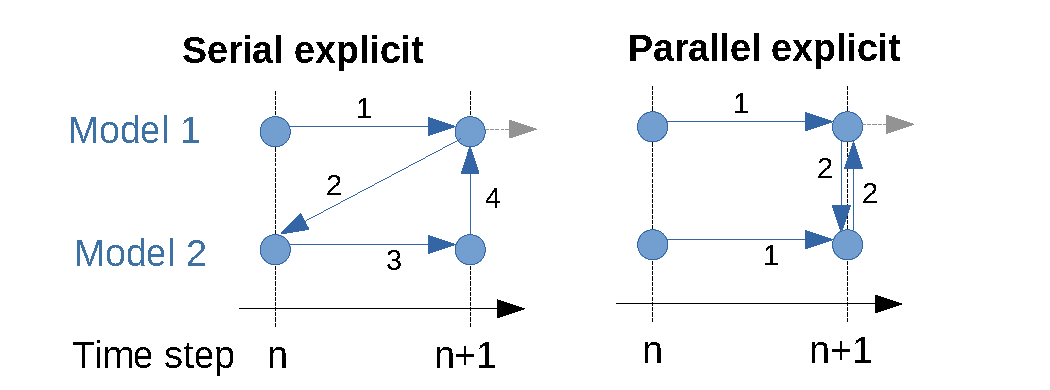
\includegraphics[width=10cm]{../figures/state-of-the-art/coupling/sequential approaches.pdf} 
\caption{Simple explicit update schemes used for multi-physics and multi-agent systems. In the serial update scheme (left), one of the models is evaluated first (1). The future state is passed to the other model (2) which uses the state for its prediction (3). The prediction is then passed back (4). In the parallel update scheme (right), the models are executed simultaneously. }
\label{fig:couplescheme}
\end{figure}


\subsubsection{Simulator coupling}
If models are located in different simulators, communication between the two simulators must be realized in addition to model coupling. 
Following approaches to exchanging data between two coupled simulators exist~\cite{gatzhammer-2014-cs}:

\begin{itemize}
\item File communication: simulators exchange data over files written to the harddisk. 
\item Socket communication: send and receive data over a network using communication protocols such as Transmission Control Protocol (TCP).
\item Message Passing Interface: intended for the communication of parallelized software in distributed systems.
\end{itemize}

The advantage of the file communication approach is that it does not require external communication libraries. The disadvantage is that the speed of the data exchange depends on the harddisk properties. If a large amount of data needs to be shared, it can take an infeasible amount of time. Therefore, file communication is often used as a fall-back solution when other communication methods fail~\cite[p.153]{gatzhammer-2014-cs}. 

Socket communication means exchanging data in a network. To manage a socket connection so-called co-simulation frameworks can be used. They manage the connecting process of the sockets and the data exchange. If a middleware is used, the simulator coupling is called `generic'~\cite{steinbrink-2017-cs}. Otherwise, the coupling is `specific', see Fig.~\ref{fig:cosimulationcoupling}. 


\begin{figure}[hbt!]
\centering
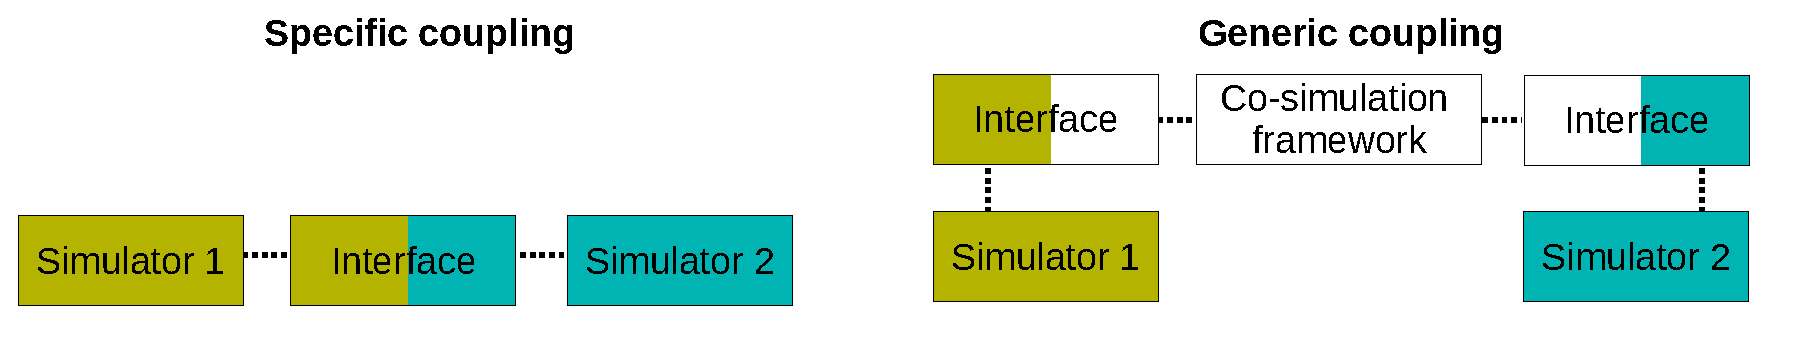
\includegraphics[width=\textwidth]{../figures/state-of-the-art/coupling/genericspecic.pdf} 
\caption[Overview on co-simulation.]{Generic and specific coupling. With a specific simulator coupling, the sockets of the simulators communicate directly over sockets in a network (left). In a generic coupling, a middleware manages the inter-process communication between simulators over sockets (right). For both types of coupling, suitable interfaces must be implemented. Own graphics inspired by~\cite{steinbrink-2017-cs}.}
\label{fig:cosimulationcoupling}
\end{figure}


\subsubsection{Validation of composite models}

Finally, I would like to briefly address the validation of composed models, assuming that the reader is familiar with the concepts of verification, validation, and calibration.  
The so-called composability theory deals with the question \enquote{[...] whether validity actually is preserved by composition. In other words, if two models are separately valid, can it be assumed that their composition is necessarily valid?}~\cite[p.63]{zhang-2019-cs}.
In his dissertation, Weisel~\cite{weisel-2004-cs} shows that a model, that is composed of two valid models, is not necessarily valid too. Only in some special cases, such as linear combinations, the composite model is valid under certain metrics~\cite{weisel-2004-cs}. 


Therefore, a composite model needs to be validated even when the component models have been validated. For this, conventional validation techniques can be used~\cite[p.76]{zhang-2019-cs}. Nevertheless, validating a model requires that empirical data is available. 



\subsection{Co-simulation frameworks and interfaces}
So far, one single crowd guidance system has been built using model and simulator coupling: CELLEVAC~\cite{lopez-2021-cdyn} for which the simulator AnyLogic was directly coupled with the commercial simulator Matlab. 

Apart from that, several middleware frameworks have been developed, see Fig.~\ref{fig:overviewcosimulation}. A middleware framework requires  to implement interfaces, see again Fig.~\ref{fig:cosimulationcoupling}. Therefore, it does not have an advantage over directly connecting simulators in terms of software engineering effort. Coupling simulators directly keeps the number of software dependencies low. For this reason, many direct couplings can be found in practice, see Tab.~\ref{tab:networkmiddleware}.


\begin{figure}[H]
\hspace*{-2cm}
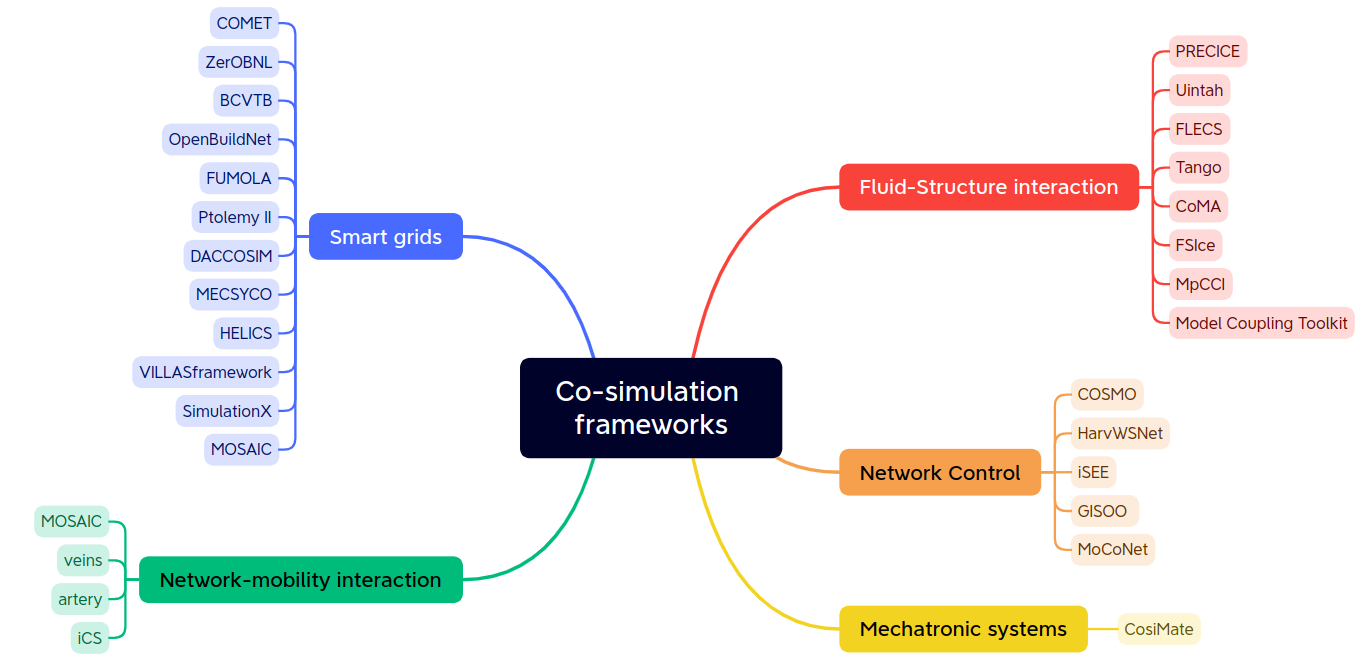
\includegraphics[width=1.2\textwidth]{./state-of-the-art/coupling/co-simulation-frameworks.png} 
\hspace*{2cm}
\caption[Overview on co-simulation frameworks]{Examples of co-simulation frameworks (middlewares). Co-simulation frameworks couple models from different simulation frameworks.
}
\label{fig:overviewcosimulation}
\end{figure}







\begin{table}[hbt!]
\centering
\begin{tabular}{lll}
 \hline 
 Framework & Mobility simulator & Network Simulator  \\ 
 \hline 
 Veins & SUMO & OMNeT++   \\ 
 Artery & SUMO & OMNeT++  \\ 
 iCS & SUMO & ns3  \\ 
 MOSAIC & SUMO, PTV Vissim & ns3, JiST/SWANS or OMNeT++  \\ 
 \hline 
 \end{tabular}  
 \caption[Simulator couplings]{Simulator couplings. The MOSAIC framework employs a generic coupling approach. Artery, iCS and Veins implement the Traffic Control Interface in the respective simulators (specific coupling). There is also one coupling with the commercial simulator PTV Vissim. }
\label{tab:networkmiddleware}
\end{table}

\newpage


For the specific coupling of mobile communication simulators and mobility simulators, the so-called Traffic Control Interface (TraCI) was introduced~\cite{wegener-2008-com}. The Traffic Control Interface couples a mobility simulator with a mobile communication simulator. The simulators exchange data over the Transmission Control Protocol (TCP). The TraCI protocol defines the structure of a message that is composed of a header and the content, see Fig~\ref{fig:tracimessage}. The content is either a request for data (How many vehicles are in the simulation?) or a command (Change the velocity of vehicle with $id=4$ to $20\,\text{km/h}$!). 


So far, only couplings  with the mobility simulator SUMO have been realized, see Tab.~\ref{tab:networkmiddleware}. The mobility models of the SUMO simulator are intended for large-scale scenarios: They cannot provide detailed trajectory data at a local scale. However, detailed data is necessary to evaluate the performance of a crowd guidance system. Therefore, the simulation frameworks listed in Tab.~\ref{tab:networkmiddleware} are not suitable for my investigations. I conclude that a novel simulation framework needs to be created that fits my needs.


\begin{figure}[hbt!]
\centering
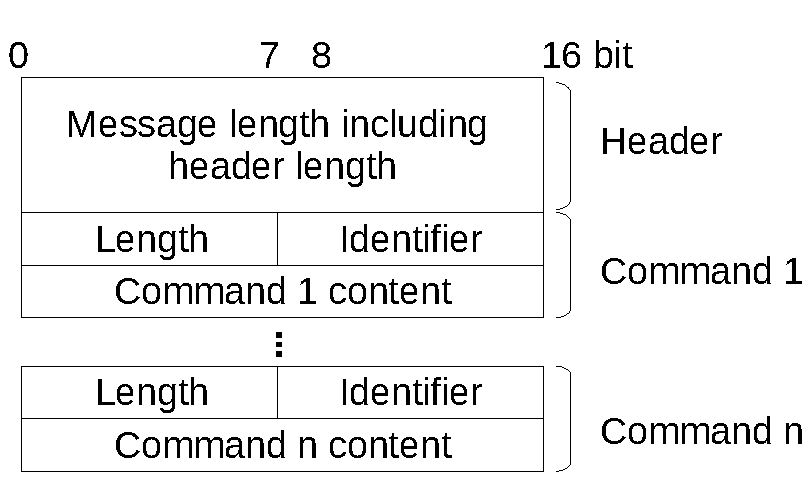
\includegraphics[width=7cm]{../figures/state-of-the-art/coupling/traci.pdf} 
\caption{Traffic Control Interface (TraCI) message. The message is communicated between the sockets of the mobile communication simulation and the socket of the mobility simulator  using the transfer communication protocol (TCP). TraCI messages are composed of a header and several commands. Own graphics inspired by~\cite{wegener-2008-com}.}
\label{fig:tracimessage}
\end{figure}






\section{Uncertainty quantification}
\label{sec:uq}
When evaluating simulation results, it is crucial to consider errors and uncertainties. Therefore, I look at uncertainty quantification methods in this section.
Several procedures exist to quantify uncertainties for which a wide theoretical foundation is available, see~\cite{smith-2014-math,xiu-2010-math}. 
One method is the Monte Carlo method~\cite{smith-2014-math}. The distribution of the uncertain parameter is approximated through a discrete sampling. The sample values are propagated through the simulation model which results in an output distribution, see Fig.~\ref{fig:uqforwardprop}. 
The Monte Carlo method requires many samples to approximate the distributions accurately, which is why applying it becomes infeasible when simulation runs take long~\cite{smith-2014-math}. This is the case for mobile network simulations that usually take several hours.
Therefore, I look at alternative uncertainty quantification methods that require less model evaluations.

In this section I look at surrogate-based uncertainty quantification with polynomial chaos expansions. I focus on two uncertainty quantification methods:
 \begin{itemize}
 \item Forward propagation: How uncertain is the model output due to uncertain parameters? 
 \item Sensitivity analysis: How influential are the uncertain parameters on the model output?
 \end{itemize}
 
The section is structured as follows: First, theory on polynomial chaos expansions is presented. In particular, it is explained how the coefficients of a polynomial chaos expansions can be determined. Then it is shown how uncertainty measures can be derived analytically from these coefficients.



\begin{figure}[hbt!]
\centering
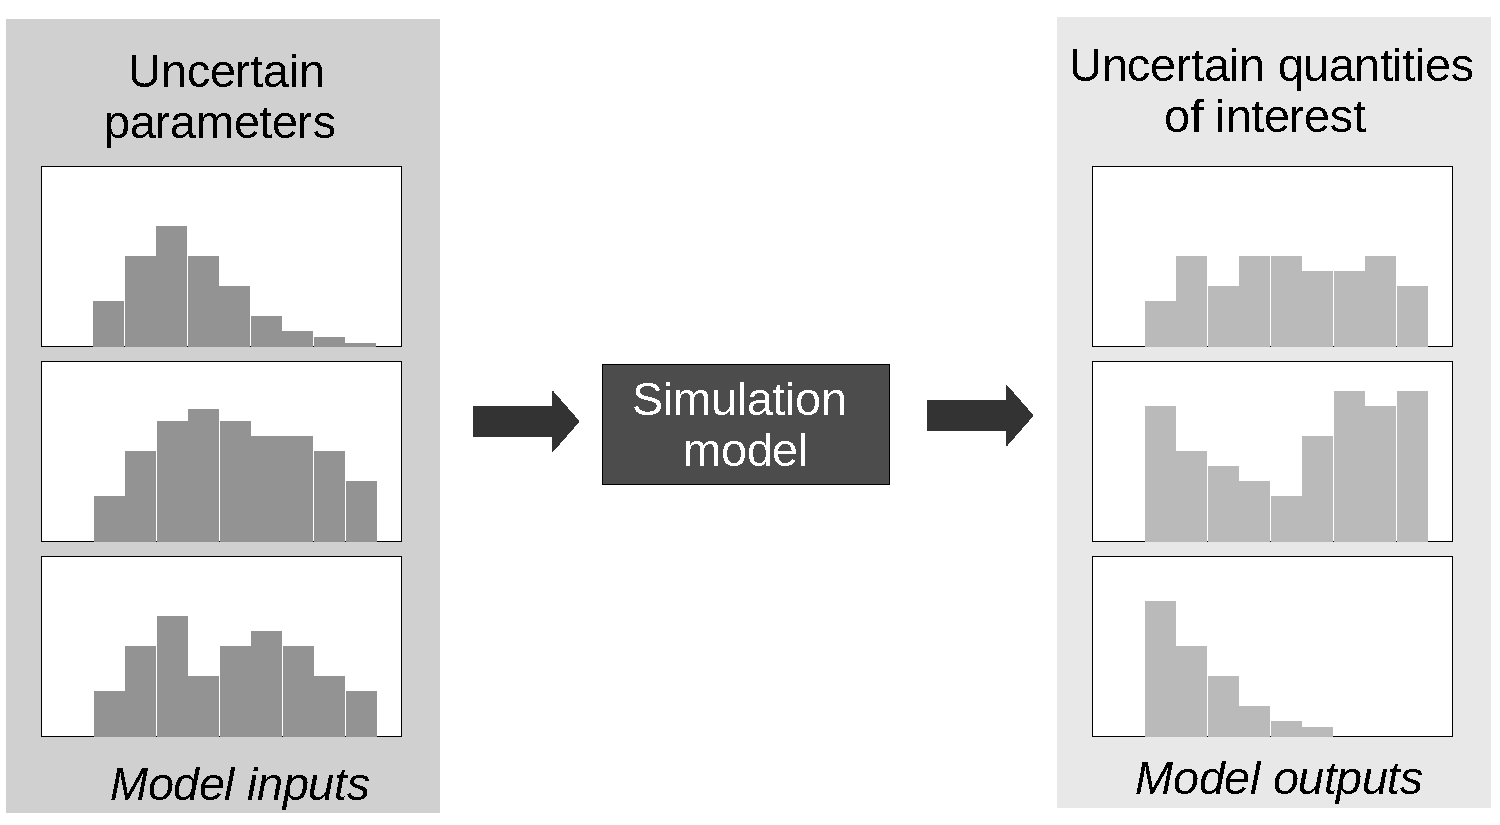
\includegraphics[width=10cm]{../figures/state-of-the-art/uq/overview.pdf} 
\caption{One method for uncertainty quantification is the Monte Carlo Method~\cite{smith-2014-math}. It can be used for forward propagation that aims to quantify the uncertainty of an output distribution. The uncertain input distributions (left) are propagated through a simulation model. Therefore, one gets an output distribution for which statistical moments can be computed. }
\label{fig:uqforwardprop}
\end{figure}



\subsection{Polynomial chaos expansion}

Polynomial chaos expansions, also known in literature~\cite{smith-2014-math} as spectral expansion, approximate an unknown model function $f$ that depends on the variable $t$ and the random variable $Z \in R^d$. Spatial, temporal, spatio-temporal, or any other deterministic dependencies are contained in $t$. The random variable $Z$ corresponds to an uncertain parameter of the simulation model $f$. A polynomial chaos expansion $f_N(t,Z)$ approximates $f(t,Z)$ using polynomial basis functions~\cite[p.67]{xiu-2010-math}:
\begin{equation}
f(t,Z) \approx f_N(t,Z) = \sum_{i \leq N}  \hat{f}_i(t) \phi_{i}(Z) \in P_N^d
\label{eg:polynmialchaosex}
\end{equation}
where $P_N^d$ is the space of polynomials of $Z$ of degree up to $N \geq 0$, $\hat{f}_i(t)$ are deterministic coefficients and $\phi_i$ are $M$ orthogonal polynomials that form a basis for the random component of the solution~\cite[p.209]{smith-2014-math}.

For any $t \in T$, the mean of $f$, denoted as $\mu_f(t)$, can be approximated by~\cite[p.67]{xiu-2010-math}:
\begin{equation}
\mu_f(t) \approx E[f_N(t,Z)] = \int \left(  \sum_{i \leq N}  \hat{f}_i(t) \phi_{i}(z)    \right) d F_Z(z) = \hat{f}_0(t)
\label{eq:meanpoly}
\end{equation}
where $F_Z(z)$ is the distribution of the random variable $Z$: $F_Z(z)=P(Z\leq z)$, see~\cite[p.64]{xiu-2010-math}.
Note that $\hat{f}_0(t)$ is the coefficient of the zero-order polynomial and has a similar function to the intercept in linear regression.

For any $t \in T$, the variance of $f$ can be approximated by~\cite[p.67]{xiu-2010-math}:
\begin{equation}
var(f(t,Z)) \approx \sum_{0  < i \leq N}  \hat{f}_i^2(t)    E[\phi_i^2(Z)]  = D_{PC}
\label{eq:varpoly}
\end{equation}

To determine the coefficients $\hat{f}(t)$, the Galerkin method, the collocation method, or the spectral method (projection) can be used. The Galerkin method is intrusive, which means that the simulation model needs to be adjusted, while the others are non-intrusive~\cite{smith-2014-math}. The spectral method requires fewer model equations than the regression-based collocation method as it only evaluates the model at particularly useful sample points. The errors of the mean and the variance convergence exponentially to zero over the number of expansion terms~\cite{xiu-2002-math}.

Each distribution type is assigned a specific polynomial type. This assignment is also known as the Wiener-Askey scheme, which extends the polynomial chaos expansions of Gaussian distributions to arbitrary distributions~\cite{xiu-2002-math}, see Tab. \ref{tab:polynomials}. The sample values are taken from quadrature tables and transformed to the respective parameter range. Therefore, the number of model evaluations equals the number of quadrature points.



\begin{table}[hbt!]
\centering
\begin{footnotesize}

\begin{tabular}{llll}
\hline 
 & Uncertain parameter $Z$ & Type of polynomial & Support \\ 
\hline 
Continous & Gaussian & Hermite & $]-\infty, \infty[$ \\ 
 & Gamma & Laguerre & $[0,\infty[$ \\ 
 & Beta & Jacobi & $[a,b]$ \\ 
 & Uniform & Legendre & $[a,b]$ \\ 
Discrete & Poisson & Charlier & $\{0,1,2,...\}$ \\ 
 & Binomial & Kryawtchouk & $\{0,1,2,...,N\}$ \\ 
 & Neg. binomial & Meixner & $\{0,1,2,...\}$ \\ 
 & Hypergeometric & Hahn & $\{0,1,2,...,N\}$ \\ 
\hline 
\end{tabular} 
\end{footnotesize}
\caption{  Distribution type of the uncertain parameter and referring type of polynomial~\cite[p.59]{xiu-2010-math}.  }
\label{tab:polynomials}
\end{table}

Standard polynomial expansions require that the model function $f$ and its derivatives are smooth~\cite{xiu-2009-math,feinberg-2018-cs}. Otherwise, the system behavior is not captured accurately due to Gibbs phenomena, that is, overshoots occur at transition points~\cite{feinberg-2018-cs}. To overcome this issue, variable transformation has been proposed: \enquote{The goal of the variable transformation is to create a new mapping which enables the response to be well approximated by a low-order polynomial chaos expansion.}~\cite{feinberg-2018-cs}. However, it is unclear how this can be implemented in practice if no information about $f$ or its differentiability is available. 


\subsection{Forward propagation and global sensitivity analysis}



Forward propagation aims to quantify the uncertainty of a quantity of interest due to uncertain parameters~\cite{smith-2014-math}. The uncertainty of the quantity of interest is quantified using the statistical moments~\cite[p.187]{smith-2014-math}. For a given polynomial chaos expansion, forward propagation cuts down to evaluating Eqs.~\eqref{eq:meanpoly}-\eqref{eq:varpoly} that describe how mean and variance depend on the coefficients of a polynomial expansion, see Fig~\ref{fig:uqexpansionstate}. 

\begin{figure}[hbt!]
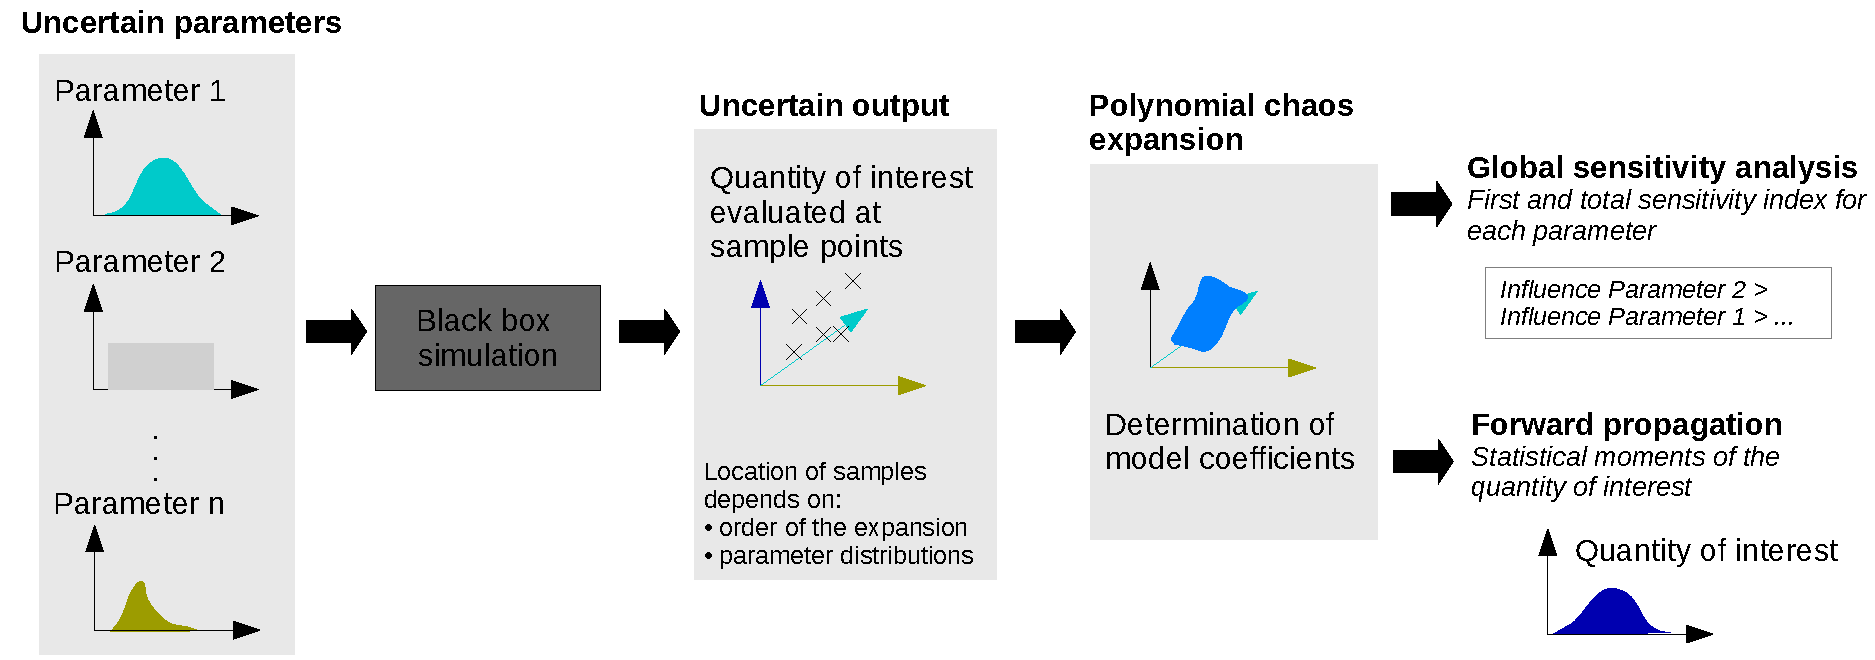
\includegraphics[width=\textwidth]{../figures/state-of-the-art/uq/polynomialchaosANDuq.pdf} 
\caption{Uncertainty quantification based on polynomial chaos expansions. Uncertain simulation parameters (left) are propagated through a black-box simulation model. The model evaluations are used to construct the polynomial expansion. With the coefficients, forward propagation and sensitivity analysis can be performed analytically. }
\label{fig:uqexpansionstate}
\end{figure}



Sensitivity analysis aims to quantify the influence of each parameter on a quantity of interest~\cite{smith-2014-math}. Global sensitivity analysis evaluates the parameter influence over the entire parameter range rather than the effect of local perturbations. One technique is the variance-based approach that can be applied to linear and non-linear functions~$f$~\cite{smith-2014-math}. The influence of each parameter on a quantity of interest~$f$ is quantified by so-called Sobol or sensitivity indices. Sudret et al.~\cite{sudret-2008-math} showed that sensitivity indices can be determined analytically from a given polynomial chaos expansion.


The first-order sensitivity index $S_i$ is defined as the ratio of the variance $D_i$ that is caused by the parameter $i$ only and the total variance $D$ of the quantity of interest:
\begin{equation}
S_i= D_i/D
\label{eq:si}
\end{equation}
The total-effect index $S_{T_i}$ is defined as ratio
\begin{equation}
S_{T_i}= D_{T_i}/D
\label{eq:siT}
\end{equation}
where $D_{T_i}$ is the variance caused by the parameter $i$ and its interactions~\cite{saltelli-2010-math} with the other parameters. The sensitivity indices can be derived analytically from its coefficients for a given polynomial chaos expansion. For this purpose, it is necessary to introduce the multivariate polynomial chaos expansion $f_N(t,\textbf{Z})$~\cite{mara-2021-math}:
\begin{equation}
f_N(t,\textbf{Z})  = \sum_{ \alpha \subset N^d}  \hat{f}_{\alpha}(t) \phi_{\alpha}(\textbf{Z})
\label{eq:multivariate}
\end{equation}
Note that the above equation is similar to Eq. \eqref{eg:polynmialchaosex} with the exception that the random variable $Z$ has been replaced by a set of random variables $\textbf{Z}$ and the index $i$ has been replaced the d-dimensional index $\alpha=\alpha_1 \alpha_2  ... \alpha_d \in N^d $ where $d$ is the number of parameters. The first sensitivity index $S_i$ can be represented as a function of the coefficients of the polynomial chaos expansions~\cite{mara-2021-math}:
\begin{equation}
S_i \approx \frac{  \sum_{ \alpha_i  > 0 }  \hat{f}^2_{ (0 ... \alpha_j ... 0) } } { \sum_{ \alpha_i  \subset  N^d}  \hat{f}^2_{\alpha} - \hat{f}^2_{(0...0)}  }
\end{equation}
Similarly, the total order indices can be represented as~\cite{mara-2021-math}:
\begin{equation}
S_{T_i} \approx \frac{   \sum_{\alpha_i  \subset  N^d: \alpha_i  > 0 }  \hat{f}^2_{  \alpha } } {  \sum_{ \alpha_i  \subset  N^d}  \hat{f}^2_{\alpha} - \hat{f}^2_{(0...0)}  }
\end{equation}
The index value evaluates the influence of a parameter. An index value of 1 means a high influence, and a value of 0 means a low influence.
Standard libraries, such as the Python package Chaospy, provide implementations for the construction of the polynomial chaos expansion and the computation of the sensitivity indices.



\section{Summary}


In this chapter I presented and analyzed state-of-the-art approaches for crowd management. A definition for crowd management was provided, differentiating it from crowd control. Then metrics for evaluating pedestrian traffic were discussed. To redirect crowds efficiently, I looked at psychological theories about crowd behavior. I found that social identities affect crowd behavior and, therefore, should be considered when providing guidance information. 


My review of crowd-sensing procedures showed that a variety of methods exist, including methods that utilize mobile communication. However, none of the approaches can measure flows or the spatial distribution of pedestrians using direct communication technology. I concluded that new methods are needed. 


The review of algorithms that compute signals to guide crowds based on current environmental information showed that the proposed algorithms were either customized to scenarios and, therefore, not transferable or were tested under the assumption that people always follow instructions, which is wrong. I concluded that algorithms are needed that can be applied to arbitrary scenarios. They should be tested under realistic conditions, that is, not all people follow instructions.


In the second part I looked at modeling and simulation approaches. My review of crowd models showed that several validated models exist for modeling the movement behavior. However, no generally applicable route choice model is available for modeling route choice behavior. Therefore, I concluded that a new modeling approach is needed to model route choice in a crowd guidance system.
In addition I found that although there are several approaches to modeling psychological behavior and communication, none of them have been used to redirect crowds in a crowd guidance system. Therefore, transferring these methods is necessary. 


Then I looked at the modeling and simulation of direct communication in mobile networks according to four mobile standards that specify direct communication: The two IEEE standards 802.11p and 802.11bd that enable direct communication in WLAN ad hoc networks, and the LTE and 5G standards of the 3rd Generation Partnership Project intended for cellular communication with or without base station that allocates resources. I looked at different modeling approaches for the radio channel and gave an overview of standardized channel models released by the mobile communication community. These models can be employed for my investigations, and no further development is necessary. 


Since a crowd management system is made up of various components, I next looked at approaches for coupling models and simulators. I presented two types of model couplings and discussed time-stepping and update procedures. I found that, due to the fact that a crowd guidance system based on direct communication technology is novel, a suitable update scheme needs to be found. Then I looked at the inter-processes communication, that is, how simulators exchange data. I found that there are middleware simulation frameworks and standardized interfaces available, but there is no simulation framework available that allows one to simulate a crowd guidance system using direct communication technology. Therefore, I concluded that a simulation framework needs to be created that I can use for my investigations. 

Finally, I presented a procedure for quantifying uncertainties in simulation results due to uncertain simulation parameters that I use in my investigations.


\chapter{Software for crowd guidance systems based on direct communication  }
\label{sec:crownet}

In this chapter I develop the scientific software \textit{CrowNet} (\underline{Crow}ds in \underline{Net}works) that I use for the investigation of my research questions in Chapter~\ref{sec:investigation}. 
The chapter is structured as follows: First I give an introduction into the simulation framework \textit{CrowNet}. I define its scope, requirements, quality measures and I present the software architecture. Since \textit{CrowNet} has been developed in collaboration with other researchers (see Appendix~\ref{sec:collaboration}), I address which parts of the software were developed by me and which parts of the software I use but which were developed by other researchers. I then go into the development of the individual modules. Some modules are based on existing simulation frameworks known from the previous chapter. I show how these frameworks have been extended for their integration into \textit{CrowNet}. Other modules provide novel models or procedures for which no software was available. I will present the respective concepts and their implementations. In this, I will focus on functionalities and features that are mandatory for the investigation of my research questions. A description of all available features of the \textit{CrowNet} framework can be found in the software documentation. At the end of the chapter I give an overview of the functionalities that \textit{CrowNet} provides for the investigation of crowd guidance systems which I will draw on in the following chapter.










\begin{tcolorbox}[float,floatplacement=hbt!,title=Availability of the simulation software]
The \textit{CrowNet} software is free and open source (LGPL-2.1 license) and publicly available on github. Please find more information in Appendix~\ref{sec:availability}.
\end{tcolorbox}





\section{Introduction to CrowNet}
\subsection{Scope}

The scope of \textit{CrowNet} is to enable the simulation of a crowd guidance system as depicted in Fig.~\ref{fig:regelkreisapplied}. The so-called controller contains the route recommendation algorithm, which provides route recommendations for redirecting the crowd at certain times. If the algorithm requires current traffic data as input, a mobile application based on direct communication technology is used as a sensor. The controller forwards the route recommendation to a second mobile application, which disseminates the information in the crowd. Importantly the recommendation for a specific time is the same for all crowd members so that groups do not split up.
The crowd reacts to a route recommendation, causing densities and flows to change. 
In the control loop, the crowd represents the dynamic system that should be influenced. Importantly, the behavior of the crowd is neither forced nor controlled. Rather, the crowd forms a system in which people can but do not have to follow instructions. This general approach allows to simulate both crowd control and crowd management applications (see~Section~\ref{sec:crowdcontroldef}). Therefore, systems --- covered by the \textit{CrowNet} software --- differ fundamentally from systems where the crowd is considered as controllable fluid. Also, they differ from navigation systems that provide route recommendations for individuals not for crowds.

\textit{CrowNet} enables the simulation of an overall crowd guidance system, an isolated sub-system and individual components. Importantly,  multiscale systems can be simulated: A crowd moves much slower than information is disseminated over the mobile network.



\begin{figure}[hbt!]
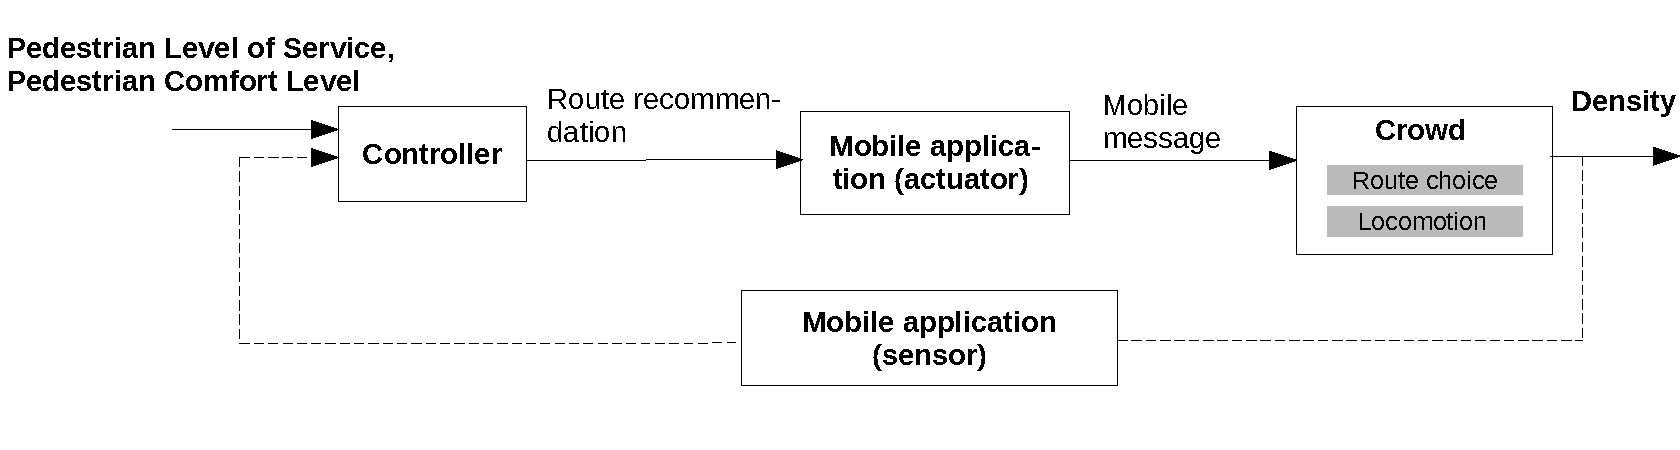
\includegraphics[width=\textwidth]{./crownet/PersonenleitsystemEinfachApplied.pdf} 
\caption[Pedestrian guidance system based on direct communication]{ Scope of \textit{CrowNet}. With \textit{CrowNet}, a crowd guidance system based on direct communication can be simulated. The crowd guidance system is represented as a control loop where the algorithm, implemented in the controller, generates route recommendations. The recommendation is disseminated through a mobile application based on direct communication (actuator). As input the algorithm uses density measurements provided by another mobile application (sensor). }
\label{fig:regelkreisapplied}
\end{figure}



\subsection{Software architecture}
\textit{CrowNet} follows a component-based architecture, see Figure~\ref{fig:architecture}. The models come from simulators and model libraries that communicate over the Traffic Control Interface (TraCI). Component models can be easily exchanged or omitted to enable the investigation of isolated subsystems. Through its modular structure it is also possible to integrate additional simulators like, for example, the SUMO simulator (see~\cite{rupp-2021-com}). 

The five main modules of \textit{CrowNet} fulfill the following purpose:




\begin{figure}[hbt!]
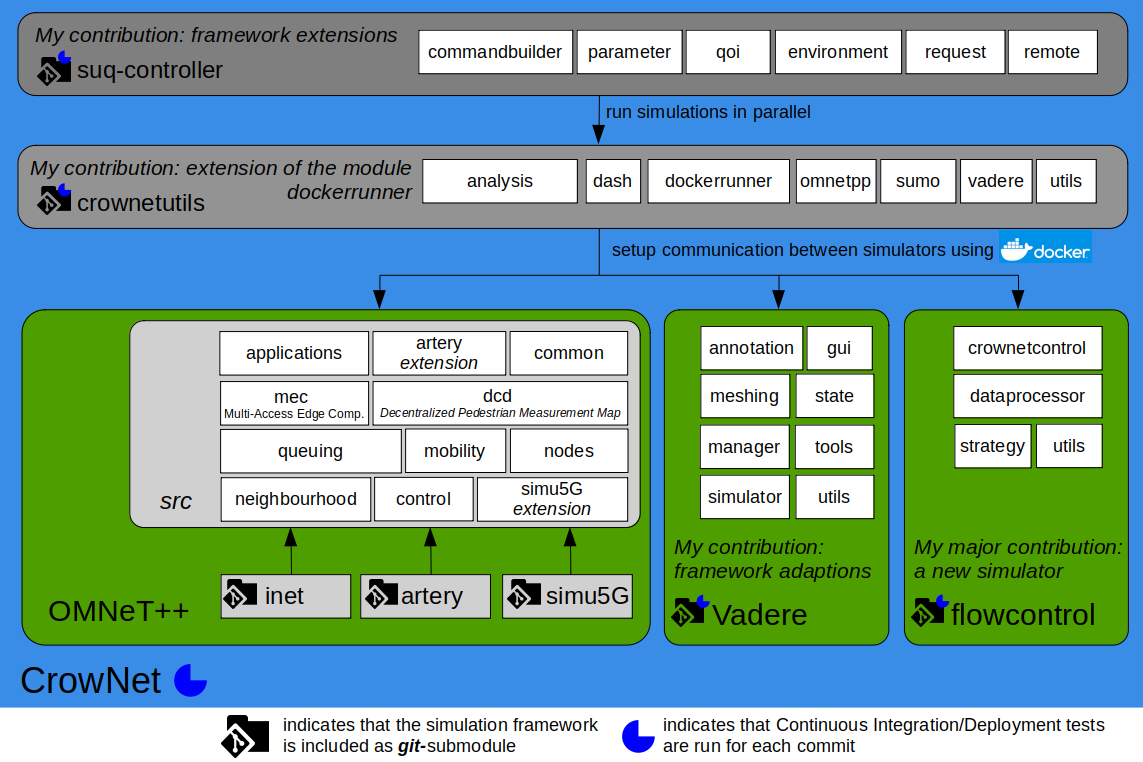
\includegraphics[width=\textwidth]{./crownet/softwarearchitecture.png} 
\caption[Software architecture of CrowNet and my contributions]{Software architecture of \textit{CrowNet} and my contributions. \textit{CrowNet} is based on several simulators that are included as modules. The \textit{OMNeT++} module (inet, artery, simu5G) provides mobile network models used to develop applications based on direct communication (src) such as sensoring crowds (dcd). The \textit{Vadere} module provides validated models for crowd behavior. The \textit{flowcontrol} modul is a novel Python simulator that provides route recommendation algorithms (my major contribution). The modules \textit{crownetutils} and \textit{SUQ-controller} enable simulations in parallel. I list my contributions for each \textit{CrowNet} module separately in Appendix~\ref{sec:collaboration}.}
\label{fig:architecture}
\end{figure}



\begin{itemize}
\item The module \textit{crownetutils} enables the execution of coupled simulations and provides pre- and post processing  methods~(Section~\ref{sec:crownetutils}).
\item The module  \textit{SUQ-controller} enables parameter studies in which coupled simulations are executed in parallel. It extends the existing \textit{SUQ-Controller} (Section~\ref{sec:suqc}).
\item The module  \textit{OMNeT++} provides new mobile applications for the detection~\cite{schuhbaeck-2021-com,schuhbaeck-2023-com} and redirection~\cite{mayr-2021-com} of crowds (Section~\ref{sec:omnet}). 
\item The module  \textit{Vadere} provides models for crowd behavior. It is based on the Vadere simulator~\cite{kleinmeier-2019-cdyn}. For its integration into \textit{CrowNet}, numerous changes were made (Section~\ref{sec:vadere}).
\item The module \textit{flowcontrol} provides route recommendation algorithms. \textit{flowcontrol} is a novel Python framework that I have developed in this thesis (Section~\ref{sec:flowcontrol}).
\end{itemize}






%
%\begin{figure}[hbt!]
%\includegraphics[width=\textwidth]{./crownet/CrownetInteraction.png} 
%\caption[Interactions in a crowd guidance system]{Interactions in a crowd guidance system.}
%\label{fig:interactions}
%\end{figure}




\subsection{Requirements, quality measures and continuous testing}
\label{sec:requirementglobal}


\subsubsection{Requirements}

The \textit{CrowNet} software is developed based on principles from software engineering. First, functional and non-functional requirements are defined, see Tab.~\ref{tab:requirementcrownetfunc}-\ref{tab:requirementcrownetnon}. The requirements define usability, testing, availability, model validity, and execution functionalities. For each requirement, a design decisions is derived that defines how the respective requirement is implemented. The design decisions listed in Tab.~\ref{tab:requirementcrownetfunc}-\ref{tab:requirementcrownetnon} are implemented in the five main modules of the \textit{CrowNet} software.  





\begin{table}[hbt!]
\begin{tabular}{|p{7cm}|p{7cm}|}
\hline
\textbf{Functional requirement} & \textbf{Design decision}  \\
\hline 
It must be possible to build a crowd guidance system according to Fig.~\ref{fig:regelkreisapplied} using existing component models. & Provide component models and manage their interaction. \\  \hline
It must be possible to exchange or extend models. & Re-use existing simulators that provide models; do not reinvent the wheel. \\ \hline
It must be possible to integrate models in novel frameworks to improve the sustainability. & Use the Traffic Control Interface~\cite{wegener-2008-com} for data exchange between simulators. \\ \hline
It must be possible to run the simulation using a single execution script. & Provide an execution script that collects all needed executables, libraries and dependencies to run a coupled simulation.  \\ \hline
It must be possible to conduct parameter studies and run simulations in parallel. & Extend the Python framework SUQ-controller (\url{https://gitlab.lrz.de/vadere/suq-controller}). \\ \hline
It must be possible to run a coupled simulation in debug mode. & Use git sub-modules that provide the source code of simulators and model libraries. \\ \hline
It must be possible to export and visualize results. &  Choose simulators with visualization and export functionalities. \\ \hline
It must be ensured that the change of a component only affects component-related properties and results. & Continuously test the software using unit and fingerprint tests. \\ \hline
The simulation framework must be accessible to everyone. & Make CrowNet publicly available on github: \url{https://github.com/roVer-HM/crownet}. \\ \hline
\end{tabular} 
\caption[]{Requirements and corresponding design decisions for functional requirements. Please see Tab.~\ref{tab:requirementcrownetnon} for the non-functional requirements. }
\label{tab:requirementcrownetfunc}
\end{table}


\begin{table}[hbt!]
\begin{tabular}{|p{7cm}|p{7cm}|}
\hline
\textbf{Non-functional requirement} & \textbf{Design decision}  \\
\hline 
The installation effort should be low. & Employ continuous deployment. Provide software components as Docker images on github: \url{https://github.com/orgs/roVer-HM/packages}.  \\ \hline
The provided component models should be validated. & Select simulators and model libraries carefully. Use libraries with validated models. \\ \hline
The provided component models should be maintained. & Select simulators and libraries that are actively maintained by checking the number of associated simulators (and forks). \\ \hline
\end{tabular} 
\caption[]{Requirements and corresponding design decisions for non-functional requirements. Please see Tab.~\ref{tab:requirementcrownetfunc} for the functional requirements. }
\label{tab:requirementcrownetnon}
\end{table}


\FloatBarrier

\subsubsection{Quality measures}

Quality measures are introduced to ensure the quality of the software, and thus, that other researchers can understand, check and use the source. The quality measures should also help to increase the sustainability of a software in the sense of Open Science (see Appendix~\ref{sec:availability}). 

I adhere to the following principles of software development:

\begin{itemize}
\item Employ a test-driven approach. I create the test method first and then implement the actual method.
\item Use a Version control system. I use git 2.25.1, which makes it possible to track the development process and jump back to older software states. This also enables researchers to reproduce study results.
\item Follow the principle of open science and make the software publicly accessible. This increases confidence in the software and avoids duplicate implementations. The code is publicly available on github: \url{https://github.com/roVer-HM/crownet}.
\item Provide releases and provide the current state of the software. I provide a stable version (release) and a main branch (current development) on github. The main branch provides new features that can be tested by external users before they are released. 
\item Follow the guidelines for clean code~\cite{martin-2008-cs}. I defined traffic engineers, crowd managers and researchers from the field of pedestrian dynamics as target groups. I use comments to explain the functionality of  classes and methods. This is mandatory as terms have different meanings between the target groups.
\item Provide documentation and tutorials. I document the code in a way that both developers and users can understand and use the code. I also provide tutorials and quick start examples.
\item Report document bugs and open tasks. I use issues boards to point out bugs and open tasks and to fix them. There is an issue board for developers and one for communication with external users that is publicly accessible: \url{https://github.com/roVer-HM/crownet/issues}
\item Apply the practice of continuous integration and continuous deployment. A push to the remote repository triggers a continuous integration pipeline, see Fig.~\ref{fig:cicd}.
\end{itemize}

\subsubsection{Testing and continuous integration}


The continuous integration pipeline consists of four stages: build, test, uq-test and deploy, see Fig.~\ref{fig:cicd}.
The build stage (1) tests whether the \textit{OMNeT++} module can be built (job: build-for-sim). It also tests whether the modules \textit{SUQ-controller} and \textit{crownetutils} can be installed in a virtual Python environment. The Python environment serves for the tests  of the following stages.

\begin{figure}[hbt!]
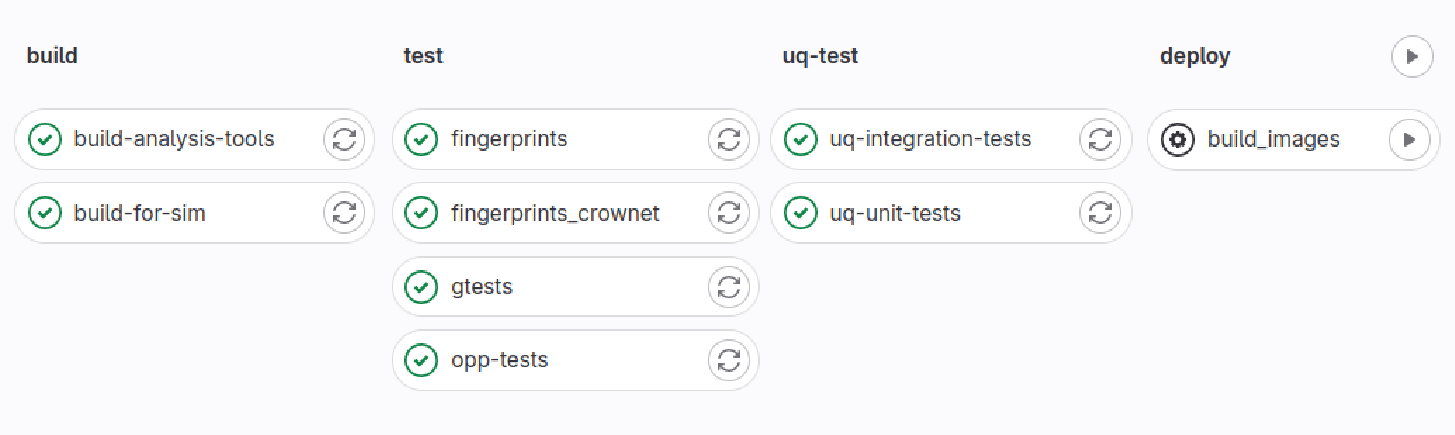
\includegraphics[width=\textwidth]{./crownet/continousintegration.pdf} 
\caption[Continuous Integration pipeline of the \textit{CrowNet} simulation framework]{Continuous Integration pipeline of the \textit{CrowNet} simulation framework. The snapshot was taken from the pipeline of the private gitlab repository. In the build stage, \textit{CrowNet} gets compiled (\lstinline{build-for-sim}) and a virtual Python environment is generated (\lstinline{build-analysis-tools}) that is used to run \textit{CrowNet} tests. The next stages contain unit tests and fingerprint tests. 
The manually triggered deployment stage (right) generates Docker images.   }
\label{fig:cicd}
\end{figure}


In the test stage (2), unit tests, regression tests, and integration tests are carried out.
For this purpose existing testing frameworks are employed: in \lstinline{opp-tests} the \lstinline{opp_test} tool of the \textit{OMNeT++} simulator~\cite{virdis-2019-com} is used to run integration tests. The \lstinline{opp_test} tool tests mobile network applications.  \enquote{Message creation and sending as well as result recording and other \textit{OMNeT++} utilities are available just like during simulation execution}~\cite[p.232]{virdis-2019-com}.
Plain C++ code is tested in a separate testing framework as recommended in~\cite{virdis-2019-com}, using the \lstinline{GoogleTest} and  the \lstinline{GoogleMock} unit testing frameworks. Note that \lstinline{gtests} stands for `google tests' in Fig.~\ref{fig:cicd}.


Regression testing is conducted to ensure that changes do not accidentally break existing functionalities: Fingerprint tests  compare a hash value computed from the simulation output with a reference fingerprint. Only if the hash values are identical, the test is successful. Fingerprint tests are available for the \textit{OMNeT++} module (\lstinline{fingerprints} in Fig.~\ref{fig:cicd}) and for the coupled simulation that includes the update scheme and the data exchange between simulators (\lstinline{fingerprints_crownet} in Fig.~\ref{fig:cicd}).


The stage \lstinline{uq-test} tests whether parameter studies can be carried out in parallel. In \lstinline{uq-unit-tests} the generation of samples is tested. Parameter studies including post-processing methods are carried out in \lstinline{uq-integration-tests}. This includes my simulation studies of Chapter~\ref{sec:investigation}. 

Docker images are used to setup and run simulations quickly and easily. The images can be  deployed in the \lstinline{deploy} stage (4) by a manual trigger. The images are generated based on the current commit. The tag of the Docker image is named after the commit for version control purposes. This  helps researchers and developers to find a specific software state for reproducing results.\textit{}





In addition to the continuous integration pipeline shown in Figure~\ref{fig:cicd}, testing is performed for each \textit{CrowNet} module. Changes in a specific module trigger the continuous integration pipeline of the corresponding module. Only if the module-specific pipeline has been passed successful, the \textit{CrowNet} pipeline (Fig.~\ref{fig:cicd}) is run in a second step. This two-step procedure simplifies and accelerates the development of individual components, as implementation errors are already detected in the module-specific tests. 

For the \textit{Vadere} module, the existing continuous integration pipeline~\cite{kleinmeier-2021-cdyn} is used. Novel pipelines are setup for the modules \textit{crownetutils}, \textit{SUQ-controller}, and \textit{flowcontrol}. As each module is integrated as a \lstinline{git sub-module} in \textit{CrowNet}, the corresponding pipelines can be triggered directly through the \textit{CrowNet} repository.



\section{Module crownetutils: model and simulator coupling}
\label{sec:crownetutils}

The \textit{crownetutils} module has the following functionalities:
\begin{itemize}
\item Configuration of the model structure of a crowd guidance system.
\item Execution of the coupled simulation.
\item Provision of pre- and postprocessing functionalities for coupled simulations.
\end{itemize} 


\subsection{Model composition and simulator coupling}
The functionalities for model composition and simulator coupling are implemented in the package \lstinline{dockerrunner} of the \textit{crownetutils} module. The core class of the package is the \lstinline{BaseSimulationRunner} that has a \lstinline{run()} method for the execution of a coupled simulation. The \lstinline{run()} method is called by the \textit{CrowNet} executable: the \lstinline{run_script}. Each simulation has its own \lstinline{run_script}, which is stored in the corresponding simulation directory, see Fig.~\ref{fig:configurationCrownet}. 

\begin{figure}[H]
\centering
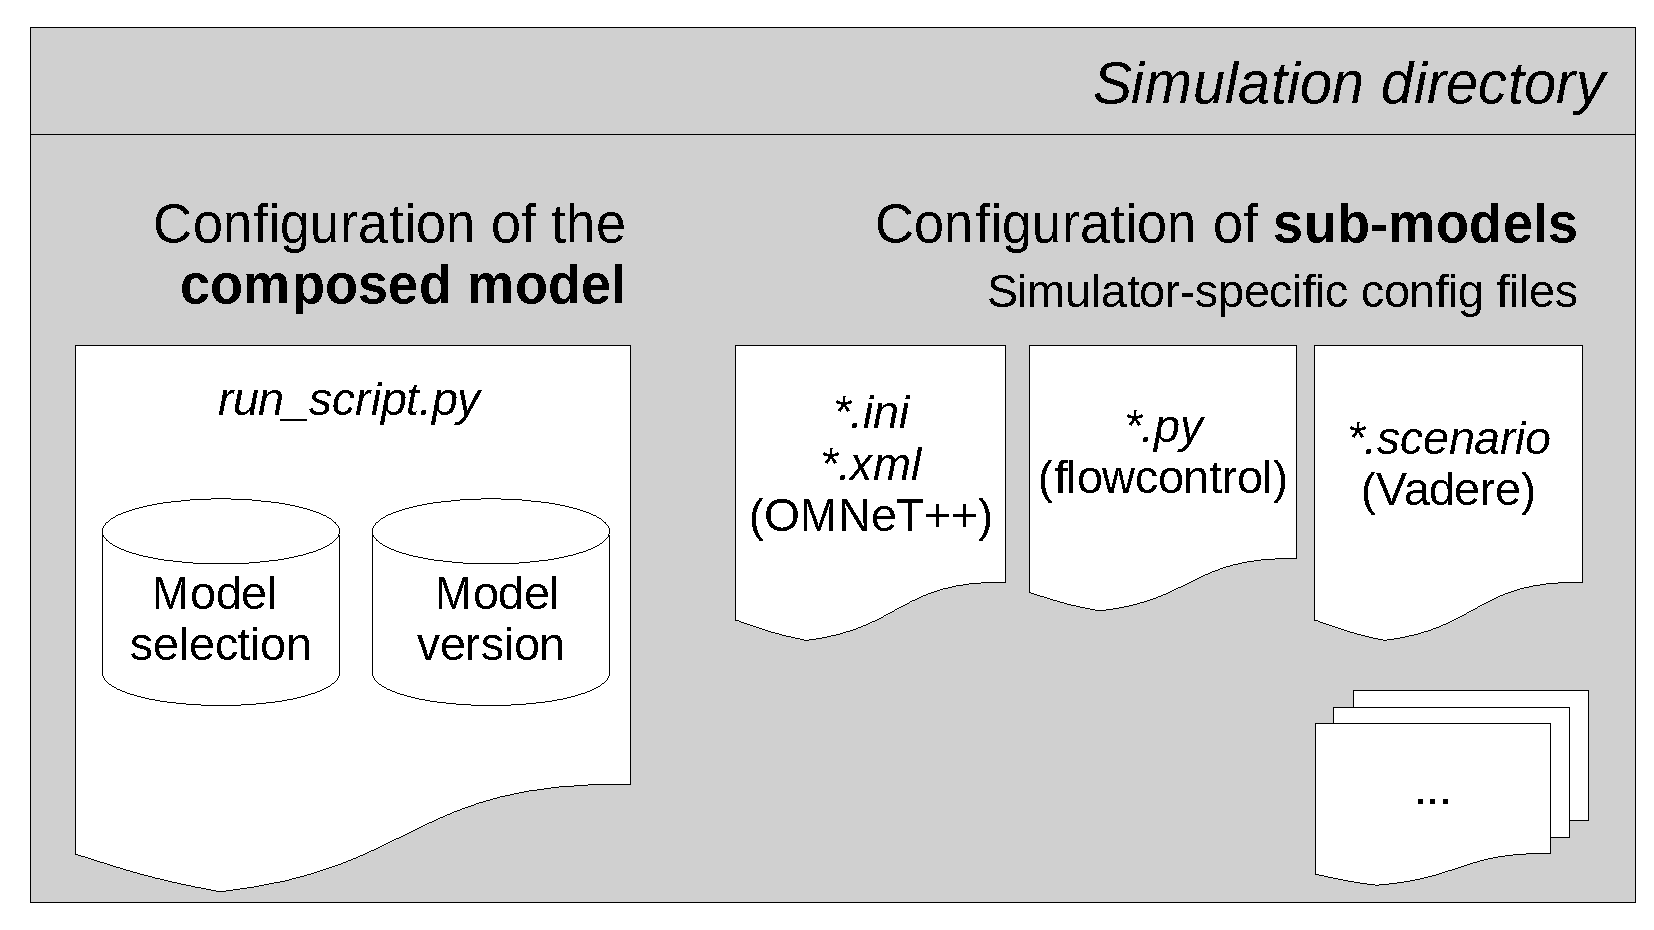
\includegraphics[width=0.8\textwidth]{./crownet/configuration.pdf} 
\caption[Configuration of a simulation in CrowNet]{Configuration of a simulation.  The model structure of the crowd guidance system is specified in the \lstinline{run_script.py}. The crowd simulation (\textit{Vadere}) is configured in the *.scenario file. The *.ini and *.xml files are config files for the mobile network simulation (\textit{OMNeT++}). The route recommendation algorithm (\textit{flowcontrol}) is specified in a Python file (*.py). }
\label{fig:configurationCrownet}
\end{figure}

The structure of the crowd guidance system is defined in the \lstinline{run_script.py}, see Listing~\ref{lst:runscript}. Parameter values are defined in the simulator-specific config files. Parameters of the crowd model are defined in the Vadere-specific \lstinline{*.scenario file}. Parameters of the communication simulator \textit{OMNeT++} are defined in the configuration file \lstinline{omnetpp.ini}. The route recommendation algorithm, implemented  the simulator \textit{flowcontrol}, is specified in \lstinline{control.py}.  Which simulator-specific files need to be included depends on the structure of the crowd guidance system.
 
\newpage



\begin{lstlisting}[caption={\lstinline{run_script.py}: executable and configuration file. Arguments specify the structure of the model and how the simulation is executed. Simulator-specific tags (--*-tag) ensure that research results can be reproduced. The tags correspond to a certain commit of the \textit{CrowNet} repository or use its current (`latest') version. },language=Python, label=lst:runscript]
from crownetutils.dockerrunner.simulationrunner import BaseSimulationRunner

if __name__ == "__main__":

    ...
    settings = [
    # configuration of the composed model
        'vadere-control', # start Vadere and flowcontrol only
        '--with-control', # specify the controller
        'control.py', # file that contains guiding strategy
        '--ctrl.controller-type',
        'AvoidShortAlgorithm', # select guiding strategy from control.py
        '--scenario-file',
        'vadere/scenarios/three_corridors.scenario', # scenario
        '--vadere-tag', # version of the docker images
        'latest',
        '--control-tag',
        'latest',
    # simulation configuration
        '--write-container-log',
        '--experiment-label',
        'myfirstcrownetexperiment',
        '--run-name',
        'sample_0', # unique name for distinguishing parallel runs
    ]
    
    runner = BaseSimulationRunner(working_dir, settings) 
    runner.run() # start the simulation
\end{lstlisting}

%\subsection{Running a coupled simulation}

In the \textit{crownetutils} module, several simulator couplings have been implemented. With this, the modeler can freely decide which parts of the crowd guidance system should be simulated.   The flexible model structure brings a performance advantage: Instead of simulating the entire system, isolated subsystems can be simulated which saves computational effort. Also it keeps the model as simple as possible. 

An overview of possible simulator combinations can be found in Fig.~\ref{fig:simulator-coupling}. The simulators exchange data using a socket communication. The crowd simulator \textit{Vadere} is always the server. The mobile communication simulator \textit{OMNeT++} is always the client. Depending on the combination of simulators, \textit{flowcontrol} acts either as a server or client.  The required simulator coupling can be selected through sub-commands that are passed over the command line interface. 

\begin{figure}[hbt!]
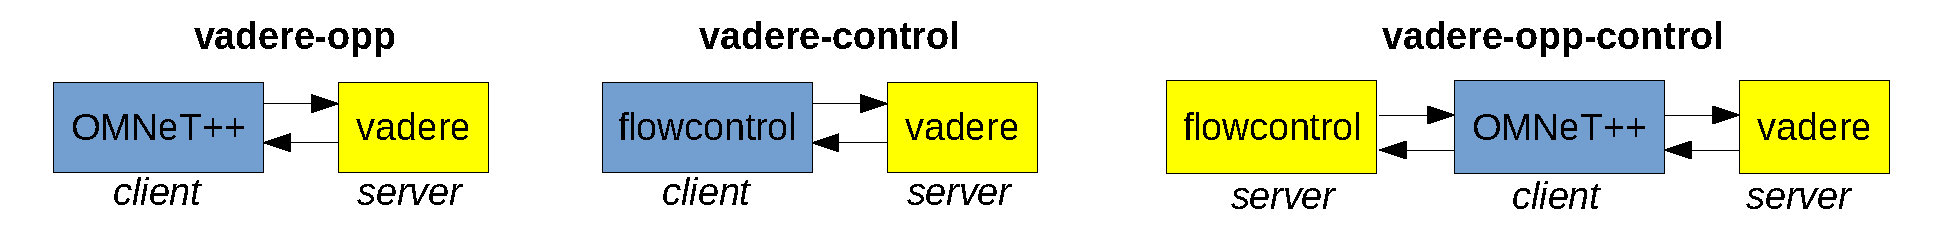
\includegraphics[width=\textwidth]{./crownet/simulationConfiguration.pdf} 
\caption[Possible simulator couplings]{Simulator couplings. The crowd dynamics simulator \textit{Vadere}~\cite{kleinmeier-2019-cdyn}, the mobile networks simulator \textit{OMNeT++}~\cite{varga-2019-com} and the novel route recommendation simulator \textit{flowcontrol} share data through socket communication.  }
\label{fig:simulator-coupling}
\end{figure}

\newpage

The execution of a coupled simulation is managed in the \lstinline{dockerrunner} module. The  \lstinline{BaseSimulationRunner} class starts the simulators in the correct order: It creates a Docker network in which the individual simulators communicate through a socket connection, see Fig.~\ref{fig:dockernetwork}. 
Using a Docker network ensures that the simulator communication processes is separated from the host network and does not influence processes of the operating system. To setup the socket connection the \lstinline{BaseSimulationRunner} first starts the server(s) that wait for the client to establish a connection. \textit{}

Each simulators is started inside the respective Docker container, see again Fig.~\ref{fig:dockernetwork}. The \lstinline{DockerRunner} of each server ensures that the simulation inside the container is ready before the next container is created. Therefore, delays during the starting process have no effect. The well-tested Python Docker API is used for the implementation. \textit{}

When coupled simulations are run in parallel, it must be ensured that the correct Docker containers connect with each other. To achieve this, the name of the Docker container is utilized as a host name. 

\begin{figure}[hbt!]
\centering
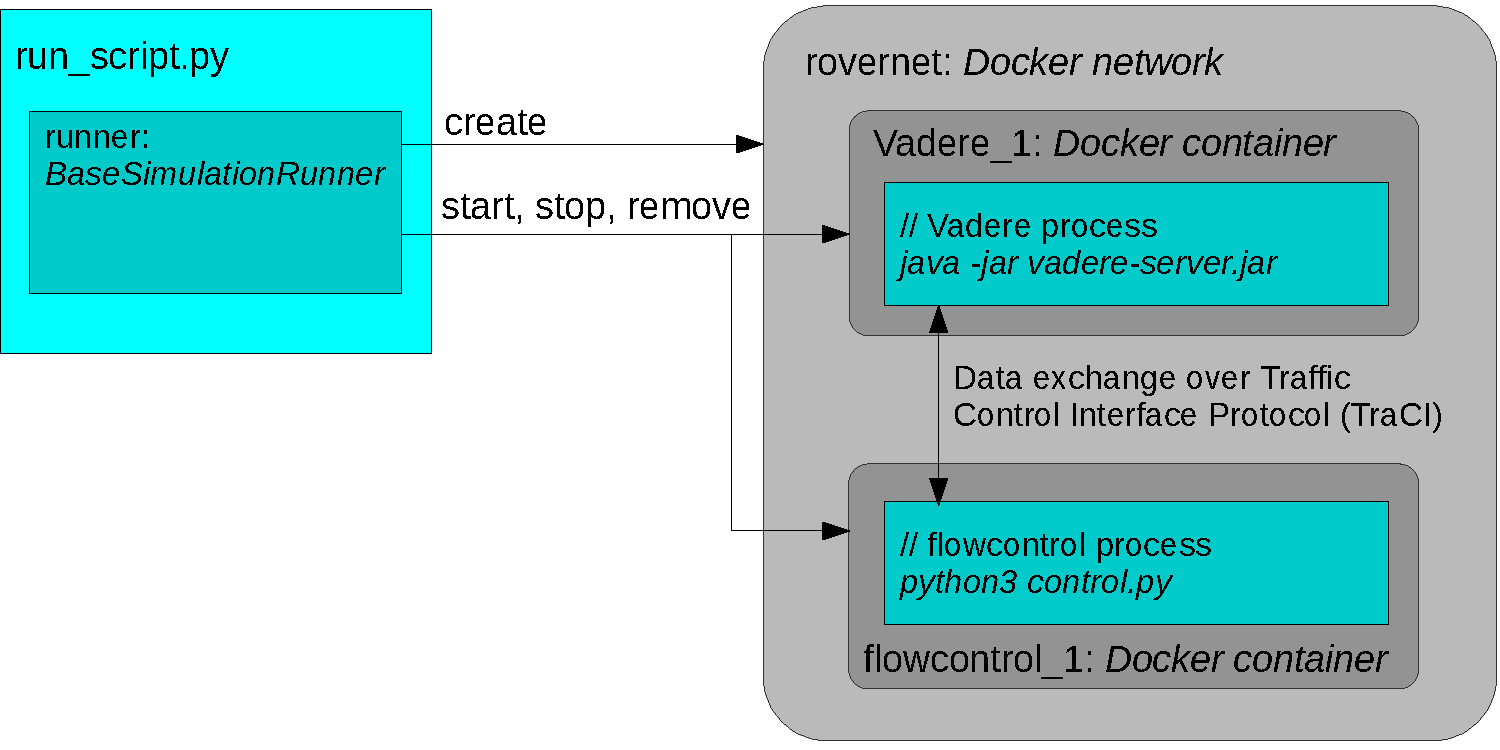
\includegraphics[width=10cm]{../figures/crownet/dockerNetwork.pdf} 
\caption{Example for simulator communication in the Docker network. The \lstinline{run_script.py} creates the Docker networks in which the simulators are executed in Docker containers that exchange data over a socket connection. \textit{}}
\label{fig:dockernetwork}
\end{figure} 


The \lstinline{BaseSimulationRunner} uses the \lstinline{SimulationDispatcher}~protocol to start and stop the required containers, see Fig.~\ref{fig:dispatcher}. The method of the \lstinline{SimulationDispatcher} protocol is selected from a sub-command provided over the command line interface. For example, if the string \lstinline{vadere-control} is passed, the method \lstinline{run_simulation_vadere_ctl()} is selected. The advantage of  decoupling dispatcher and runner is that further simulator couplings can be easily implemented, while at the same time, all classes implementing the respective methods can be called through the \lstinline{SimulationDispatcher} protocol. To start a simulation the main method of the \lstinline{run_script.py} calls the run method of \lstinline{SimulationRunner}. Therefore, the \lstinline{run_script.py} has a dual function: Configuring the model structure and executing the simulation.

Once a socket connection has been established, the simulation states are exchanged via the Traffic Control Interface (TraCI)~\cite{wegener-2008-com}. In the \textit{Vadere} simulator the Traffic Control Interface was implemented in \cite{schuhbaeck-2019-com}. \textit{Vadere} has the role of the server and waits for requests that are provided via the network, see Fig.~\ref{fig:vaderesequence}. \textit{OMNeT++} and \textit{flowcontrol} use subscriptions to request the simulation state from the other simulator. 


\begin{figure}[hbt!]
\centering
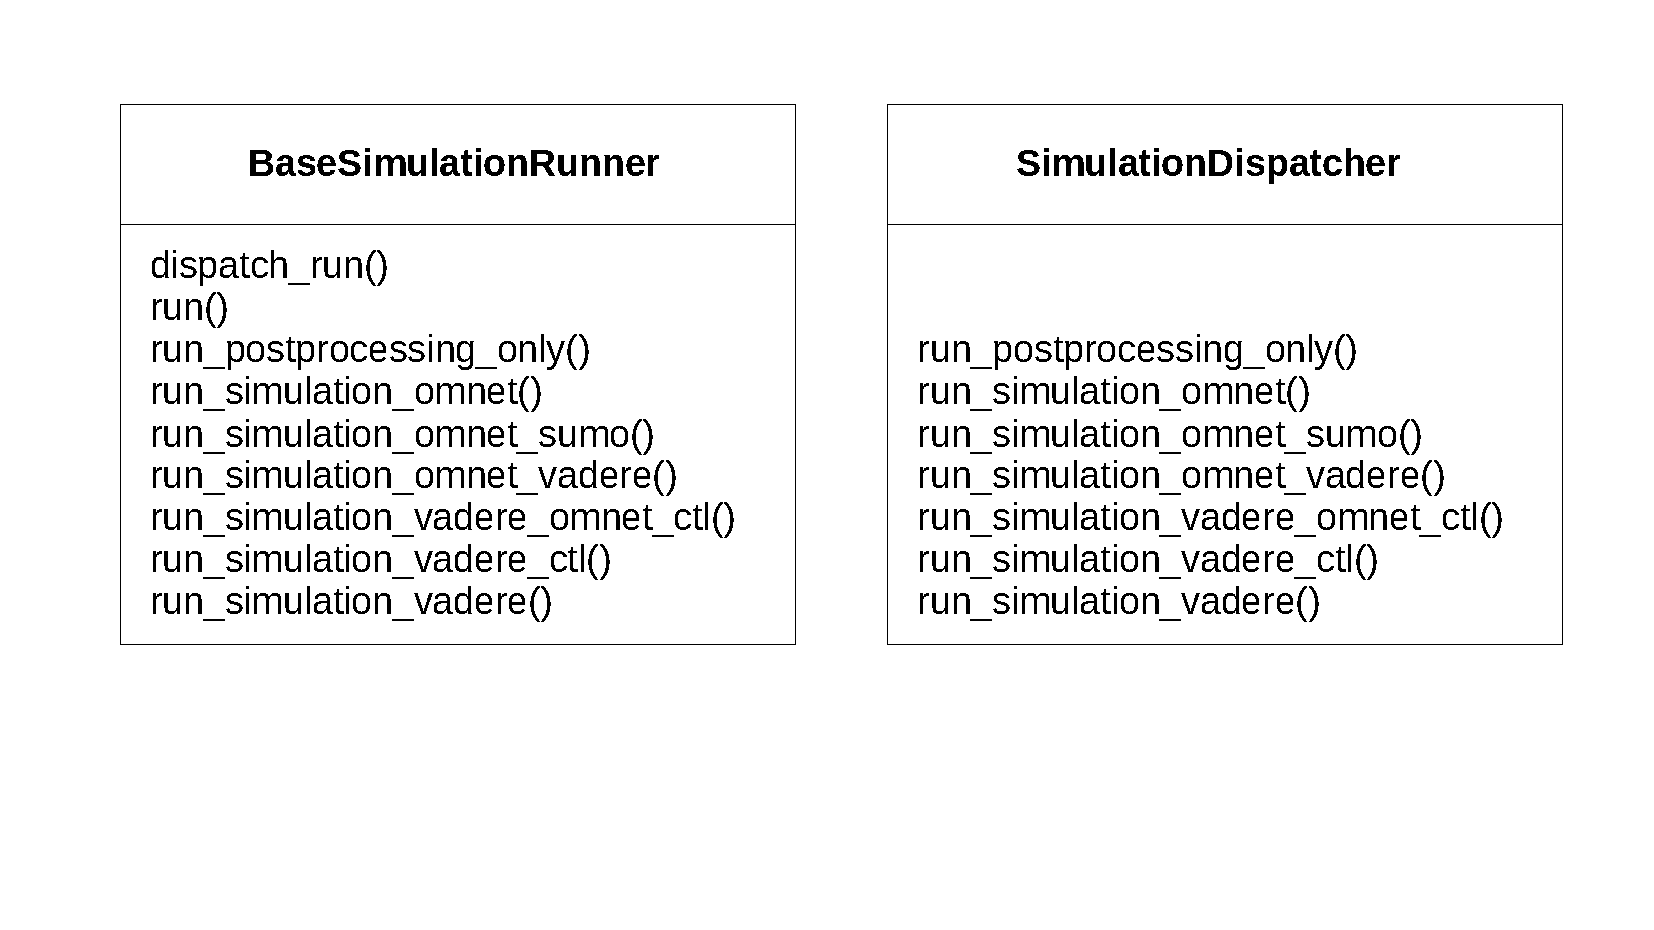
\includegraphics[width=10cm,trim={0cm 4.8cm 0cm 1.25cm},clip]{./crownet/crownetutilsDispatcher.pdf} 
\caption[SimulationRunner and Dispatcher: simplified class diagramms]{\lstinline{SimulationRunner} and \lstinline{SimulationDispatcher}: simplified class diagrams. }
\label{fig:dispatcher}
\end{figure}





\begin{figure}[H]
\centering
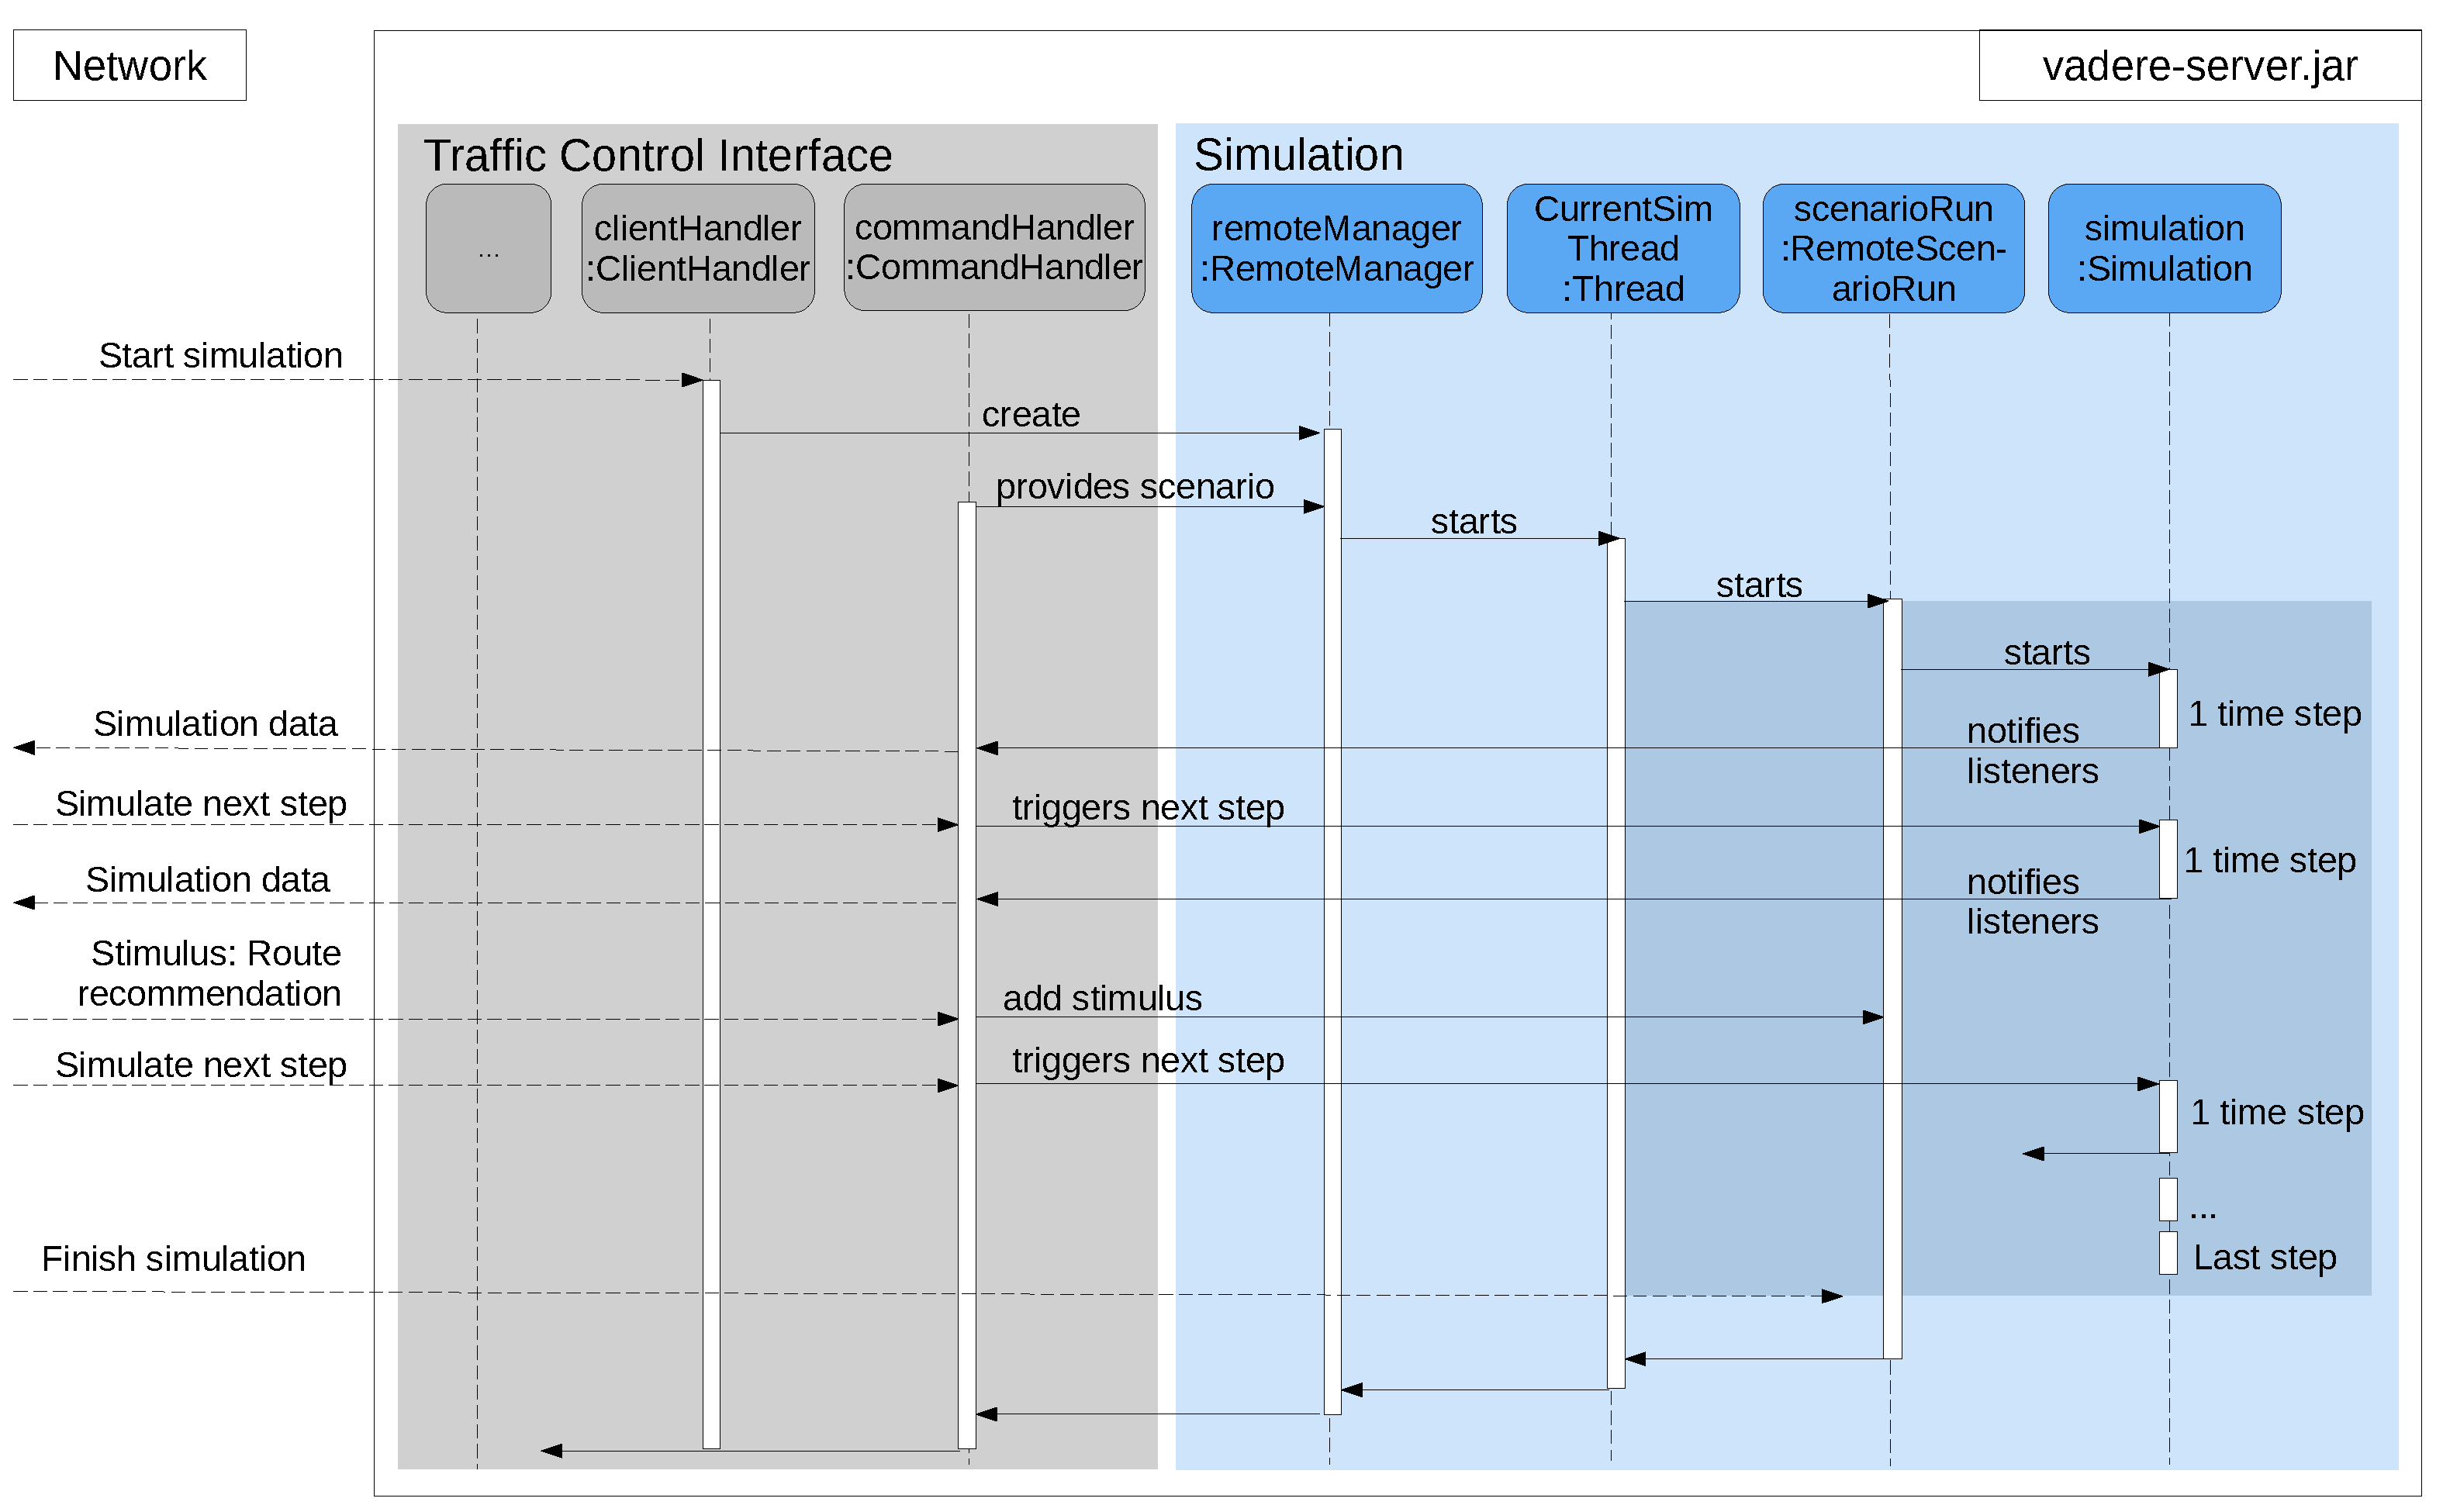
\includegraphics[width=0.85\textwidth]{./crownet/vadere_traci_implementation.pdf} 
\caption[Processes in Vadere during coupled simulation]{Traffic Control Interface and simulation loop of \textit{Vadere}. The interface was implemented in~\cite{schuhbaeck-2019-com} to enable a communication with the mobile network simulator \textit{OMNeT++}.}
\label{fig:vaderesequence}
\end{figure}



\FloatBarrier


\subsection{Explicit update scheme with position interpolation}
\label{sec:explicite}
An explicit update scheme is implemented to update the state of the component models, see Fig.~\ref{fig:updateschemecrownet}. The global time step size corresponds to the time step size of the crowd simulator \textit{Vadere}. \textit{Vadere} provides mobility data for the simulator \textit{OMNeT++}.

\begin{figure}[hbt!]
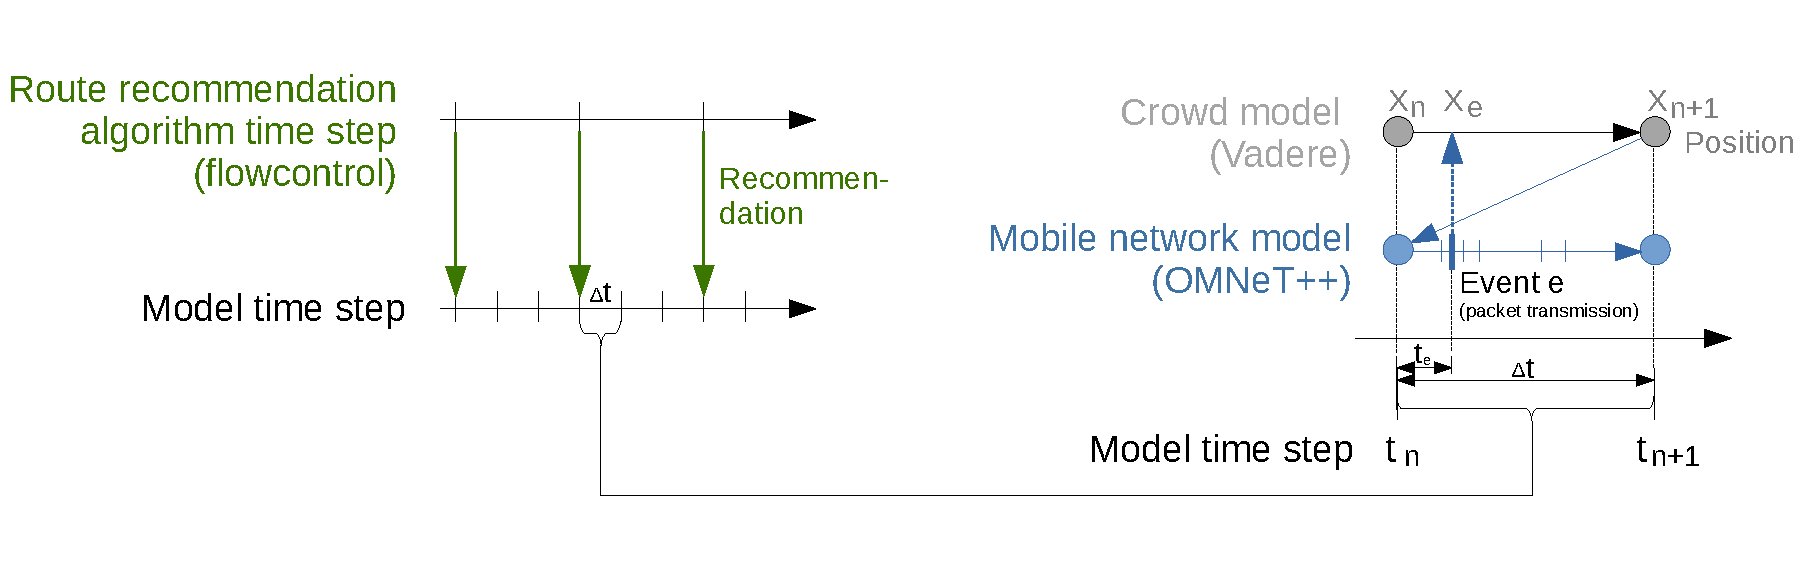
\includegraphics[width=\textwidth]{../figures/crownet/updateapproach.pdf} 
\caption{Explicit update scheme with position interpolation. The route recommendation algorithm, the crowd model and the mobile network model exchange data at certain times. The route recommendation algorithm provides route recommendations every $m$ time steps with $m \geq 1$ (left). The position data in the mobile network simulation is interpolated linearly (right). }
\label{fig:updateschemecrownet}
\end{figure}

In \mbox{\textit{OMNeT++}}, the position of agents is interpolated using the current and the future state. The route recommendation algorithm (\textit{flowcontrol} simulator) is evaluated every $m$ time steps where $m \geq 1$.  



The interpolation of the agent position is exact if the node velocity of an agent (i) is constant within one time step. The speed of an agent (i) is estimated from the current and future node position:
\begin{equation}
v^i = \left\{
\begin{array}{ll}
\frac{X_{n+1}^i -  X_n^i}{\Delta t}  & n > 1 \\
0 & \, n = 1  \\
\end{array}
\right. 
\end{equation}
where $n \in \mathbb{N}^+$ denotes the time step, $X^i$ denotes the position of agent (i), and $t_e$ is the time in between the event and the time $t_n$.
%
The position of agent (i) at a specific point in time (e) is:
\begin{equation}
X_e^i = X_n^i + v^i t_e 
\end{equation}

Importantly, there is no physical coupling between the mobile network simulation and the crowd simulation. Only the current agent positions play a role in the mobile networks simulation. Therefore, one can  assume that the update scheme does not lead to any stability problems. I check this in my investigations.
\textit{}

\subsection{Pre- and Postprocessing methods}

The \textit{crownetutils} module provides a feature with which pre- and post-processing methods can be implemented. Is is based on annotations, see \lstinline{process_as} in Listing~\ref{lst:prepost}. The pre- and post-processing methods are selected using the command line parameter \lstinline{--qoi} of the \lstinline{run_script} . Each pre- and post-processing method is assigned a priority value to specify the order of execution: see the properties \lstinline{type} and \lstinline{prio} in Listing~\ref{lst:prepost}. The higher the \lstinline{prio}, the sooner the method is executed. The package \lstinline{analysis} provides implementations of standard metrics for the evaluation of the mobile communication simulation.

\begin{lstlisting}[caption={Adding pre- and postprocessing to a \textit{CrowNet} simulation using annotations.},language=Python, label=lst:prepost]
from crownetutils.dockerrunner.simulationrunner import BaseSimulationRunner, process_as

class SimulationRun(BaseSimulationRunner):

    @process_as({"prio": 1, "type": "pre"}) # before sim start
    def prepare_1(self):
        ...        

    @process_as({"prio": 1, "type": "post"}) # after sim finished 
    def result_1(self):
        ... 
        dataframe.to_csv(result_1.csv)
    
    @process_as({"prio": 2, "type": "post"}) # after sim finished 
    def result_2(self):
        ...
        dataframe.to_csv(result_2.csv)
\end{lstlisting} 


\section{Module SUQ-Controller: extensions for coupled simulations}
\label{sec:suqc}

The \textit{SUQ-controller} module builds on the \underline{S}urrogate and \underline{U}ncertainty \underline{Q}uantification \underline{controller} (SUQ-controller) that is an open source Python framework for executing parameter studies in parallel, see Appendix~\ref{sec:availability}.  The \textit{SUQ-controller} was intended for conduction parameter studies with \textit{Vadere}. It created a copy of \textit{Vadere}'s config file (*.scenario) for each sample and overwrote the parameter values.

In \textit{CrowNet}, however, the simulation is specified via several configuration files. In addition, simulators are coupled. Therefore, the \textit{SUQ-controller} needs to be extended for conducting  parameter studies with coupled simulations.






\subsection{Enabling coupled simulations through new process calls}
The \textit{SUQ-controller} is extended to execute coupled simulation by introducing the new module \lstinline{CommandBuilder}, see Fig.~\ref{fig:commandbuilder}. The core of the module is the class \lstinline{Command}.

\begin{figure}[hbt!]
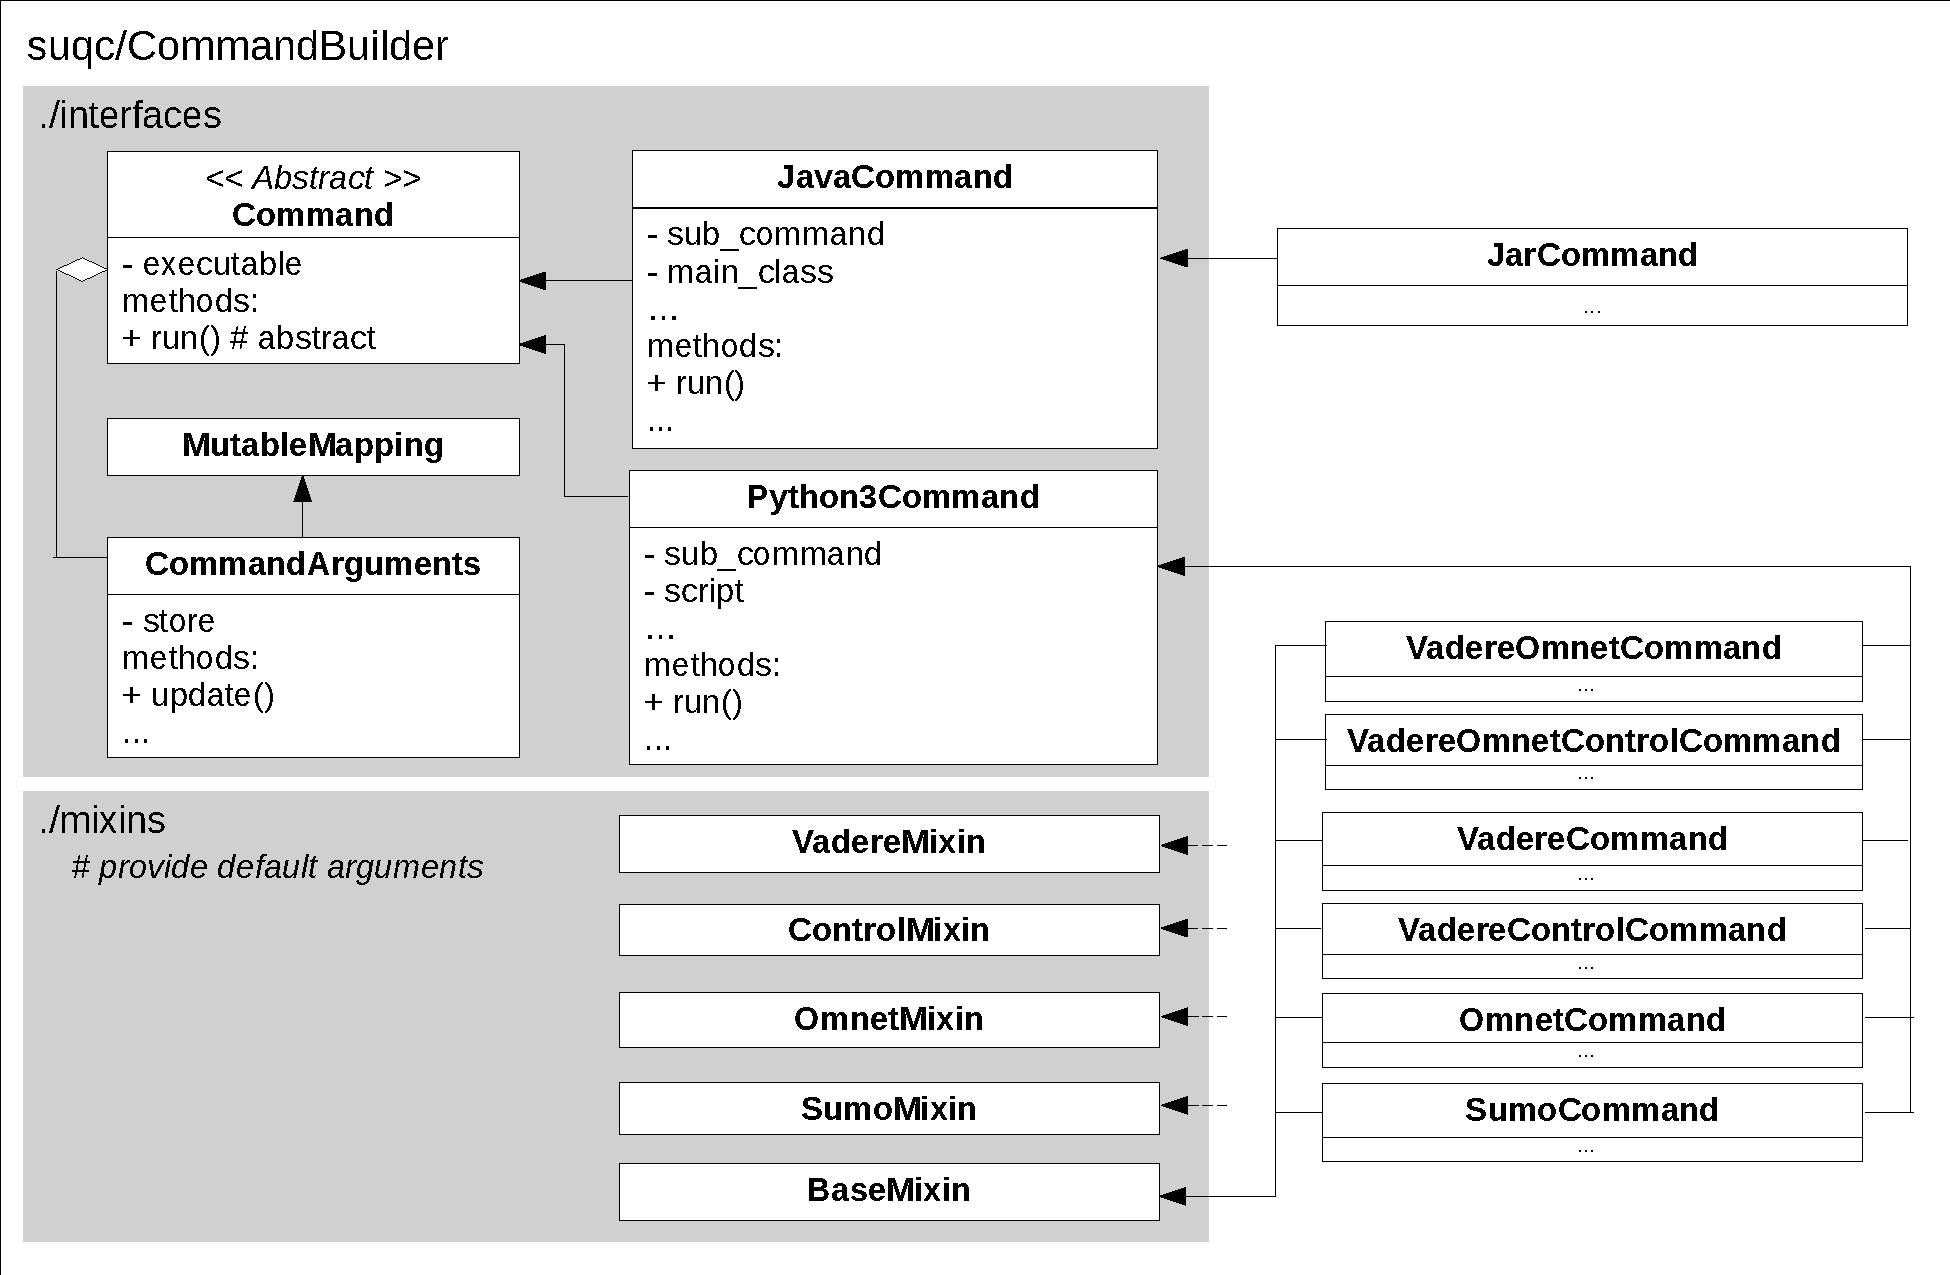
\includegraphics[width=\textwidth]{./crownet/suqc-commands.pdf} 
\caption[SUQ-Controller: sub-package CommandBuilder]{Extension of the SUQ-Controller: The module \lstinline{CommandBuilder} provides commands to conduct simulation studies with coupled simulations. }
\label{fig:commandbuilder}
\end{figure}

The \lstinline{Command} class defines how an executable is started. It has two child classes: \lstinline{JavaCommand} and \lstinline{Python3Command}. The former relates to Java executables, such as \lstinline{vadere-console.jar}. The latter specifies Python executables, such as \lstinline{run_script.py}. Each child class implements a corresponding \lstinline{run()} method. The \lstinline{run()}  method of the \lstinline{JavaCommand} child class is used to start the \textit{Vadere} application via the command \lstinline{java -jar vadere-console.jar}. 

The \lstinline{run()} method of the \lstinline{Python3Command} class calls the \lstinline{runscript.py}. \lstinline{Python3Command} has numerous child classes,  see Tab.~\ref{tab:wrappercommands}. With the different child classes, parameter studies can be conducted with individual components, isolated subsystems or the entire crowd guidance system.

The child classes inherit from the \lstinline{mixins} package, see again Fig.~\ref{fig:commandbuilder}. The \lstinline{BaseMixin} class defines general simulation settings such as the log level. The simulator-specific  \lstinline{mixins}  enable the configuration of simulator releases and simulator-specific settings.


\begin{table}[hbt]
\begin{tabular}{p{6cm}p{7.5cm}}
\hline 
Command  & Parameter study with \\ \hline
 {VadereOmnetControlCommand}& ... a crowd guidance system according to Fig.~\ref{fig:regelkreisapplied}.\\
VadereOmnetCommand &  ... a crowd guidance system without dynamic route recommendation provision. \\
VadereControlCommand& ... a crowd guidance system without mobile communication. \\
 {OmnetCommand}, {VadereCommand} & ... an individual component of a crowd guidance system.\\
\hline
\end{tabular} 
\caption{Child classes of the \lstinline{Python3Command}. They serve as wrapper commands.}
\label{tab:wrappercommands}
\end{table}












\subsection{Executing parameter combinations in parallel}
The simulator-specific config files (see again Fig. \ref{fig:configurationCrownet}) contain the model parameters. To conduct a parameter study, the parameter values in these files need to be changed. The \textit{SUQ-controller} reads the respective config files and parses them into a dictionary. 
To parse the *.ini file of the \textit{OMNeT++} simulator, the Python package \textit{omnetinireader} has been developed, see Appendix~\ref{sec:availability}. It is open source and is included as external library in the \textit{SUQ-controller}. 

Parameters of the \textit{flowcontrol} simulator are changed over the \lstinline{--controller-type} argument that is passed to \lstinline{run_script.py}. The \textit{SUQ-Controller} requires that parameter values are stored as a list of dictionaries. Each list element corresponds to one sample. The parameter values are specified for each simulator separately, see Listing~\ref{lst:sample}. 


\begin{lstlisting}[caption={Sample definition (Python dictionary) in a coupled simulation.},language=Python, label=lst:sample]
sample = {'omnet': { "*.misc[0].app[0].repeatInterval": "1.0s",
                   "**wlan[*].radio.transmitter.power": "2.0mW" },
         'vadere': {"sources.[id==1].spawner.distribution.updateFrequency": 2.0}}
\end{lstlisting}

Since the \textit{Vadere} and \textit{OMNeT++} simulators contain stochastic processes a \lstinline{SeedManager} is implemented, see Fig.~\ref{fig:seedmanager}. It generates reproducible seed values that are fed into \textit{Vadere} and \textit{OMNeT++}. 

The execution of a parameter study with coupled simulators is shown in Fig~\ref{fig:sequencesuqc}. The executable is defined via a \lstinline{Command} object. The parameter combinations are passed as a list of dictionaries to the \lstinline{Command} object. The \textit{SUQ-controller} then creates simulation directories and manages the execution of simulations in sub-processes. To reduce the overall runtime, the processes are started in parallel. To ensure that simulator instances are correctly assigned, the Docker containers receive a post-fix with the corresponding sample number: The container \lstinline{flowcontrol_Sample_00} only communicates with the containers \lstinline{omnet_Sample_00} and \lstinline{vadere_Sample_00} but not with \lstinline{vadere_Sample_01} or \lstinline{omnet_Sample_02}.




\begin{figure}[H]
\centering
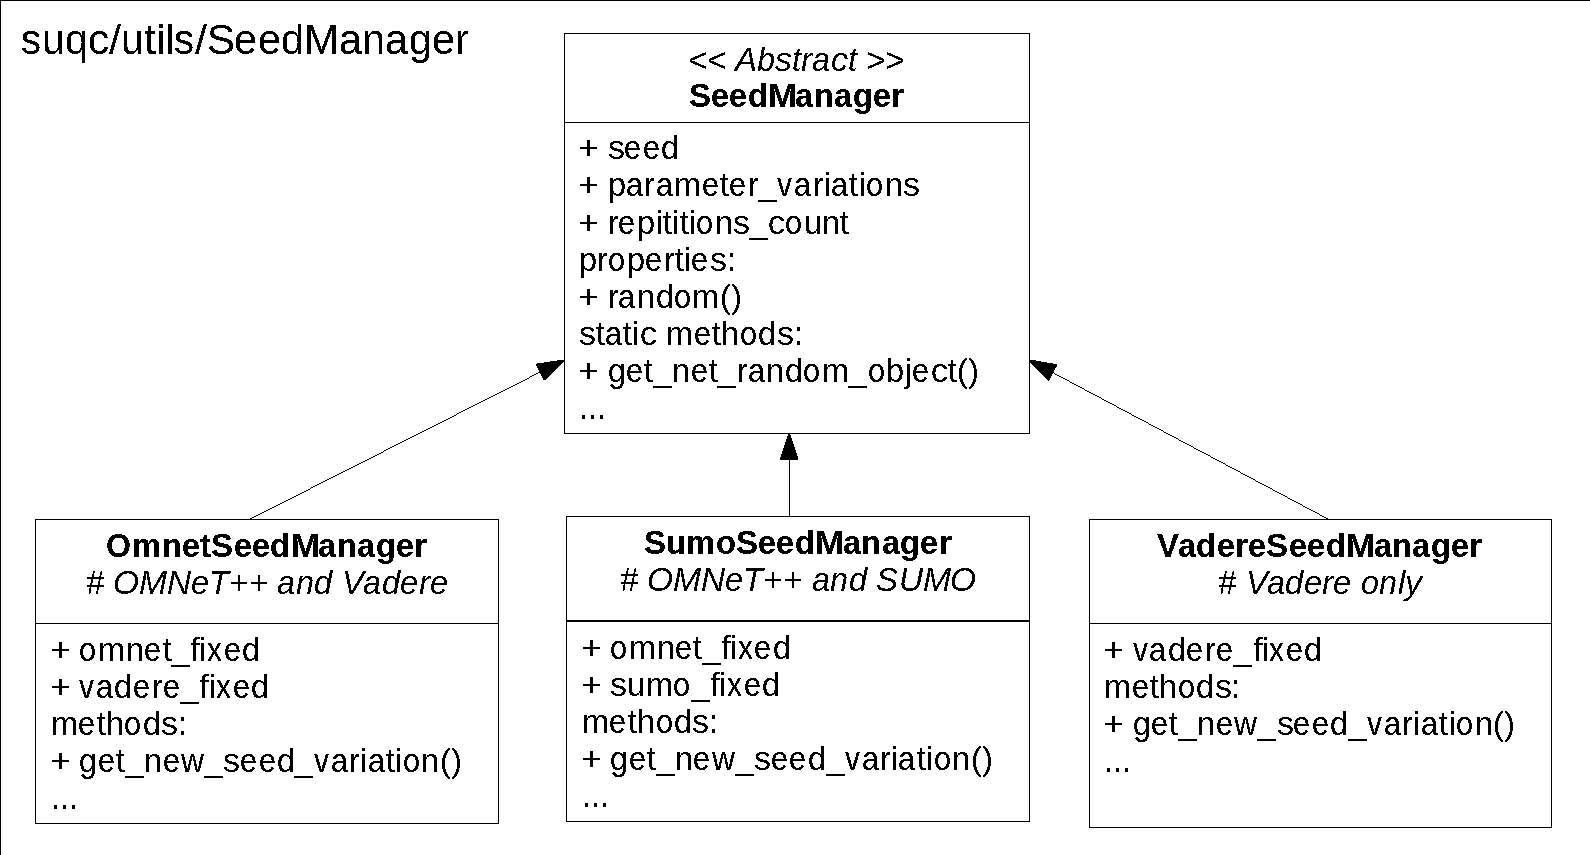
\includegraphics[width=0.95\textwidth]{./crownet/suqc-seed-manager.pdf} 
\caption[SUQ-Controller: sub-package SeedManager]{\lstinline{SeedManager} of the \textit{SUQ-controller} module. Seeds are generated and fed into the \textit{OMNeT++} simulator and the \textit{Vadere} simulator. This ensures that the repetition of stochastic simulations leads to the same results.}
\label{fig:seedmanager}
\end{figure}
\begin{figure}[H]
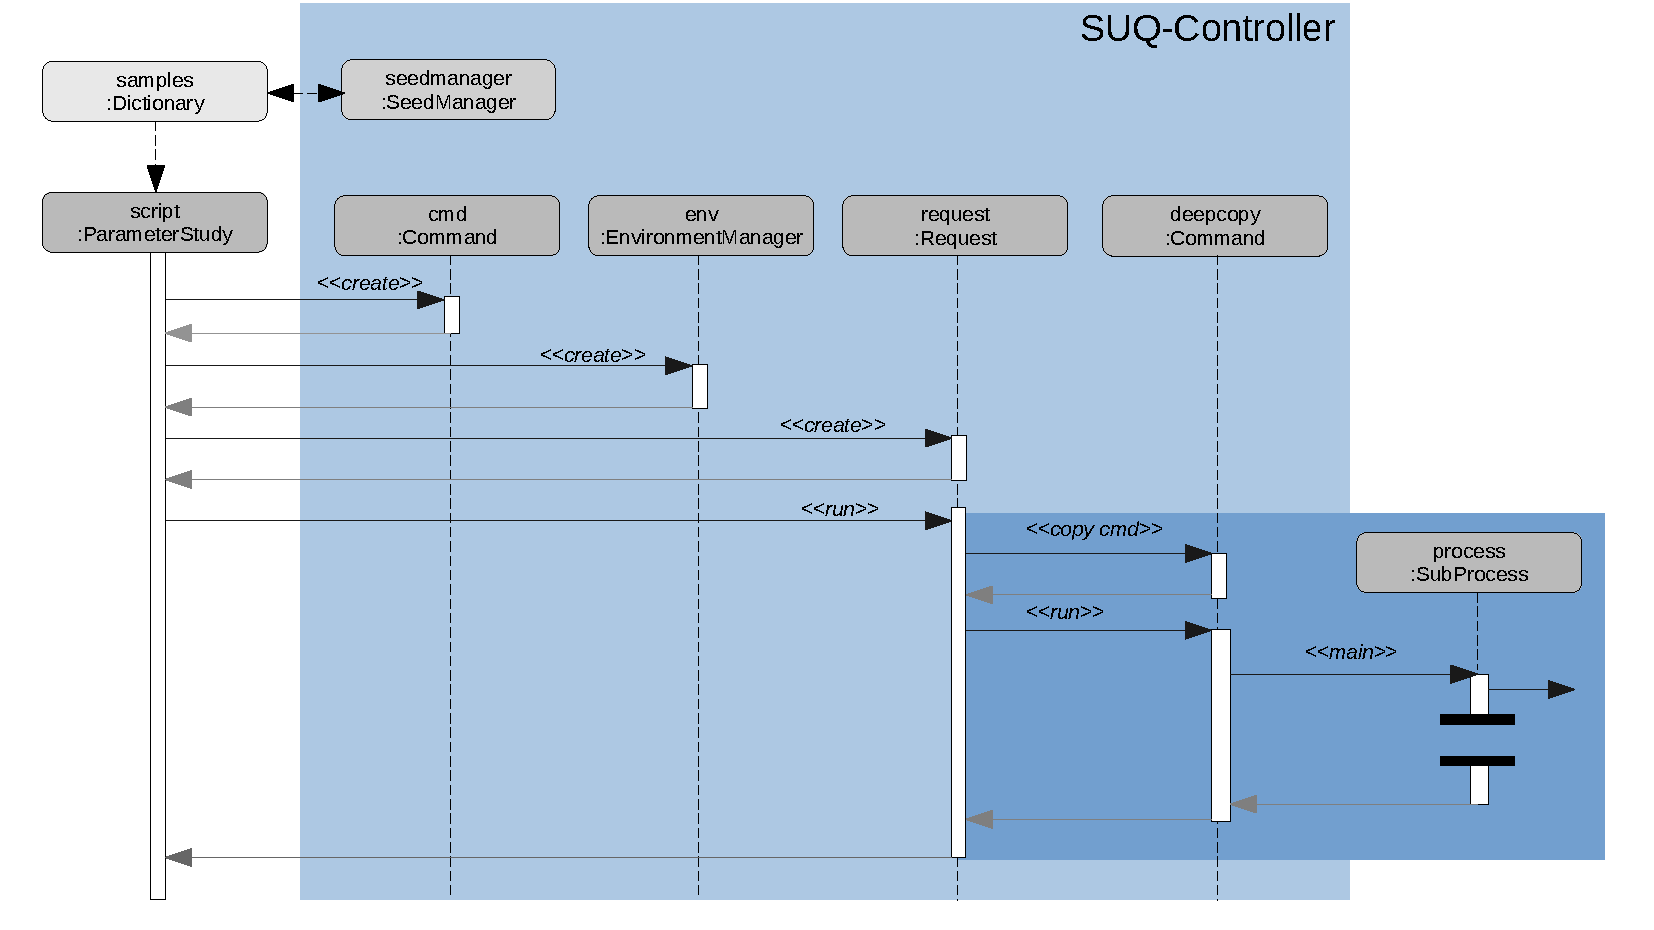
\includegraphics[width=1\textwidth]{./crownet/suqc-sequence.pdf} 
\caption[Sequence diagram of a ]{Conducting a parameter study using the \textit{SUQ-controller} module. The \lstinline{SeedManager} generates seeds for the samples. Before the simulation is started in a sub-process, several objects are generated that specify or manage the simulation (\lstinline{cmd}, \lstinline{env}, \lstinline{request}).}
\label{fig:sequencesuqc}
\end{figure}

 

\section{Module OMNeT++: provider for direct communication}
\label{sec:omnet}

The \textit{OMNeT++} module provides mobile network models and executes the mobile network simulation. It contains implementations of crowd sensing procedures and mobile applications that disseminate information based on direct communication. I use the module, but I did not contribute to it.


\subsection{Employing OMNeT++ and its ecosystem}

In the \textit{OMNeT++} module, several frameworks are integrated to simulate direct communication. The frameworks have been developed externally and have inter-dependencies, see Fig.~\ref{fig:packagedeps}. Some of them enable the simulation of WLAN-based communication and some others enable cellular communication. All frameworks are based on the \textit{OMNeT++} simulation engine for the execution of their models. The \textit{Vadere} crowd simulator was integrated in the \textit{OMNeT++} ecosystem in 2019~\cite{schuhbaeck-2019-com}. The aim was to provide  realistic pedestrian mobility data for the mobile communication simulation.

\begin{figure}[hbt!]
\centering
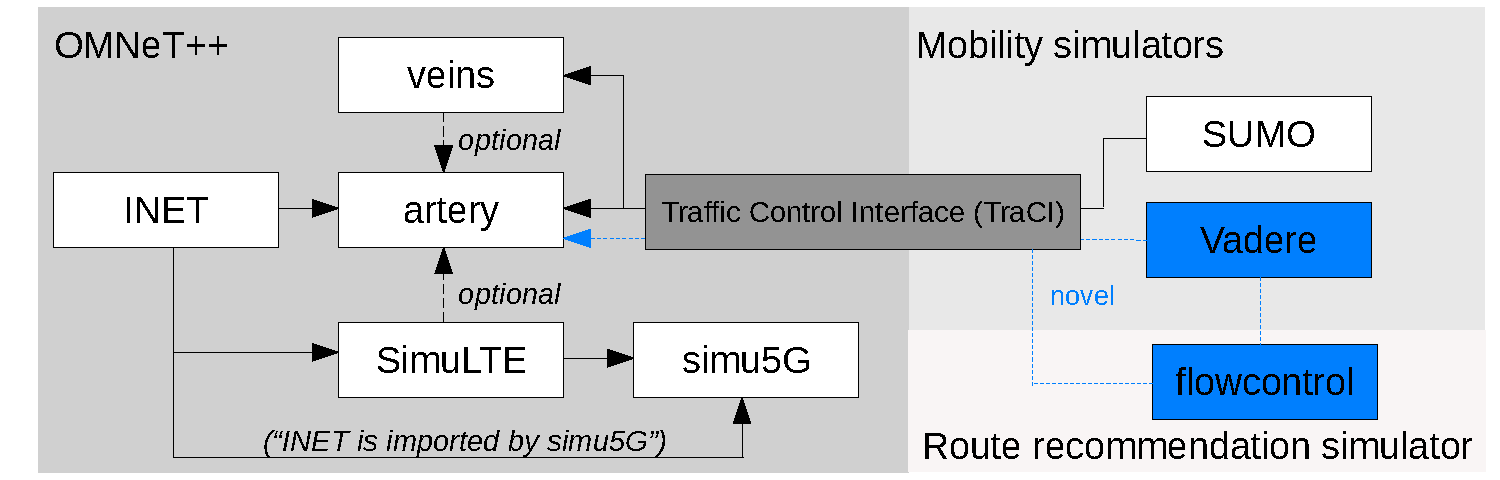
\includegraphics[width=\textwidth]{../figures/crownet/frameworkdependencies.pdf}
\caption{Package dependency of the \textit{OMNeT++} module. The \textit{OMNeT++} simulation engine is related to several simulators and model libraries. Only simulators that are integrated in the \textit{OMNeT++} module are depicted (\textit{inet}, \textit{artery}, \textit{SimuLTE}, \textit{simu5G}, and \textit{Veins}).
The pedestrian dynamics \textit{Vadere} was integrated in~\cite{schuhbaeck-2019-com}. The novel simulator \textit{flowcontrol} is integrated as part of this thesis. Own graphics inspired by~\cite[p.369]{virdis-2019-com}. }
\label{fig:packagedeps}
\end{figure}

The \textit{OMNeT++} module is named after the simulation engine \textit{OMNeT++}~\cite{varga-2019-com}. The engine is event-based and intended for arbitrary distributed systems.\textit{OMNeT++} is licensed under the Academic Public Licence. The core of \textit{OMNeT++} is the C++ simulation kernel that handles the execution of event-based simulations. This includes the processing of input files, the scheduling of events, collecting results, and handling the optional online visualization. \textit{OMNeT++} has a generic component architecture. Model components are termed `modules' that \enquote{communicate via message passing, either
directly or via predefined connections. Messages may represent events, packets, commands, jobs, or other entities depending on the model domain}~\cite{varga-2019-com}. So-called simple modules use the simulation class library and are implemented in C++. Modules can represent different objects, such as agents, sinks generating network traffic, or network interface cards.  So-called compound modules  are composed of at least two simple modules. They represent more complex systems such as hosts or routers. For the setup of the network topology so-called Network Topology Description (NED) files are used. Model parameters and simulation kernel settings are defined in the *.ini file.
 


The \textit{{INET}} framework~\cite{meszaros-2019-com} serves as model library for the simulation of direct communication according to the 802.11p standard. \textit{INET} is an established library that contains standard communication protocols for network simulations. It is licensed with the LGPL license and is used in research, academia, and industry. 
\textit{INET} has started out as \enquote{a model suite for the Internet protocol stack (e.g., IPv4, TCP, and UDP), and has gradually expanded to other areas, in particular: Ethernet, IEEE 802.11, QoS mechanisms, MPLS, DiffServ, Internet routing protocols, node mobility, MANET routing protocols, further wireless MAC protocols, IPv6, and SCTP, just to name a few. Recent advancements include physical layer and physical medium modeling, advanced visualization features, and improved network emulation capabilities.}~\cite{meszaros-2019-com}.  \textit{INET} provides transceiver models including antenna, models for the transmission medium and obstacle and terrain models. Each model can be individually configured or extended. The simulation frameworks  \textit{simuLTE, simu5g} and \textit{artery} --- all used by the OMNeT++ module  --- build on \textit{INET}. See again Fig.~\ref{fig:packagedeps}.


The \textit{simuLTE}~\cite{virdis-2014-com} framework and the \textit{simu5G} framework~\cite{nardini-2020b-com} enable the simulation of direct communication in cellular networks.
\textit{{simuLTE}} is a system-level simulator that enables the simulation of 4G LTE and Long Term Evolution Advanced (LTE-A) networks. It also serves as a model library for node models and base stations. \textit{simuLTE} provides the full LTE protocol stack that is composed of the physical layer, the medium access layer, the Radio Link Control (RLC) and the Packet Data Convergence Protocol (PDCP).  The provided receiver models consider simultaneous transmissions in the computation of the Signal-to-Interference-plus-Noise-Ratio (SINR) which allows the analysis of interference. \textit{simuLTE} enables infrastructure-mode communications and sidelink communications in mode 3 (controlled mode) where the base station allocates resources. \textit{{simu5G}} extends the \textit{simuLTE} framework by enabling the simulation of 5G networks. The source code of \textit{simuLTE} is fully provided in the \textit{simu5G} framework. Like \textit{simuLTE}, \textit{simu5g} only supports the controlled mode (mode 3), that is, resources are allocated by a base station while data is exchanged over sidelinks.


\newpage



The \textit{{veins}}~\cite{sommer-2011-com} framework is an open source library that provides models for vehicular communication according to the 802.11p standard. It provides models for the IEEE 802.11p Medium Access Control (MAC) layer, the IEEE 1609.4 Multi-Channel, and the IEEE 802.11p physical layer. For the upper layers, it uses the WAVE architecture that is used in the United States. Veins does not provide any models for modeling the mobility behavior of vehicles, but accesses position data from the SUMO simulator via the Traffic Control Interface (TraCI). The coupling via the Traffic Control Interface is bi-directional. With this, one can simulate traffic rerouting~\cite[p.218]{virdis-2019-com}.


Like \textit{veins} the \textit{{artery}}~\cite{riebl-2015-com,riebl-2019-com} framework enables vehicular communication. It was originally intended as a module of the \textit{veins} framework. Meanwhile \textit{artery} has become a separate framework licensed under the GPLv2 license. \textit{artery} builds on models provided by the \textit{INET} framework. It extends the 802.11p physical and access layers with ad-hoc mode functionalities. The scope of \textit{artery} is the simulation of application scenarios in European countries. Hence, the radio channel bandwidth and the carrier frequency are set to frequencies of $10\,\text{MHz}$ and $5.9\,\text{GHz}$. Like \textit{veins}, \textit{artery}  uses the Traffic Control Interface for receiving mobility data. \textit{artery's} implementation of the Traffic Control interface is used for the data exchange with the simulators \textit{flowcontrol} and \textit{Vadere}.





\subsection{Pedestrian density map application for crowd sensing}
\label{sec:novelapplication}

The package \lstinline{applications} provides implementations of mobile applications. One of them is the `decentralized pedestrian density map application' that was first proposed in \cite{schuhbaeck-2021-com} and further developed in \cite{schuhbaeck-2023-com}. The application aims to measure the spatial and temporal distribution of the density of people based on a cell-grid, see Fig.~\ref{fig:densitymap565242}.

\begin{figure}[hbt!]
\centering
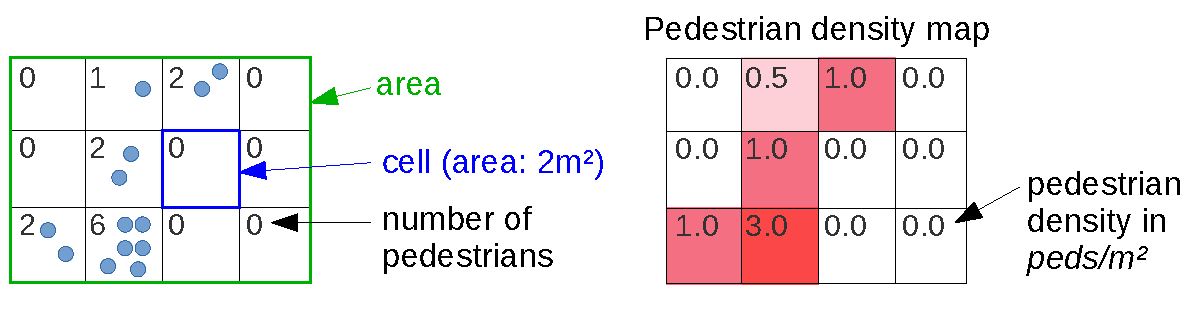
\includegraphics[width=0.8\textwidth]{./crownet/app-density-map.pdf} 
\caption[Decentralized pedestrian density map]{Decentralized pedestrian density map. The topography is discretized with a cell-grid. The  density is estimated from the number of received beacons per cell. The beacons are assigned to a specific cell via a position date.
}
\label{fig:densitymap565242}
\end{figure}

The idea of the density map application is to count people by counting 4G/5G sidelink beacons~\cite{schuhbaeck-2021-com}.  
Devices regularly send beacons with position data via the so-called beacon service, see Fig.~\ref{fig:services-crowdsensoring}. 
Each device counts the number of received beacons for each cell. Based on the count and the cell size, the  density can be derived for each cell. 
Since the range of a beacon is limited, the position data is only locally available.
To receive density information from distant cells, density data is exchanged between devices over a second service: the density map service.  The density maps are aggregated to improve the accuracy of densities, see Fig.~\ref{fig:aggregation}.


Both beacons and density map application packets communicate using 4G/5G sidelink communication~\cite{schuhbaeck-2023-com}. Because each device counts itself, the pedestrian counting is both local and decentralized. Data flow and storage times are, therefore, not covered by data protection~\cite{moencke-2023-com}. 

The density map application has been tested in simulation studies for LTE in the controlled mode (mode 3)~\cite{schuhbaeck-2023-com}. In the study the authors used a base station with 25 resource blocks and a carrier frequency of 2.6 GHz in combination with a heuristic path loss model~\cite{itu-2012-com}. Two filter algorithms were proposed for the aggregation of the count data~\cite{schuhbaeck-2023-com}:

\begin{itemize}
\item Youngest measurement first. For each cell, sort the estimated values according to their age. Use the most recent estimate.
\item Youngest measurement first plus distance. For each cell, normalize age and distance (distance between the cell and the cell of the device that estimated the number of persons) to values between 0...1. Calculate a weighted mean from the normalized values (suitable weights: 0.9 for the normalized age and 0.1 for the normalized distance, see~\cite{schuhbaeck-2023-com}). Use the estimated value that is assigned to the smallest weighted mean.
\end{itemize}
If no beacon has been received for a cell, it is assumed that the cell is not occupied.


\begin{figure}[hbt!]
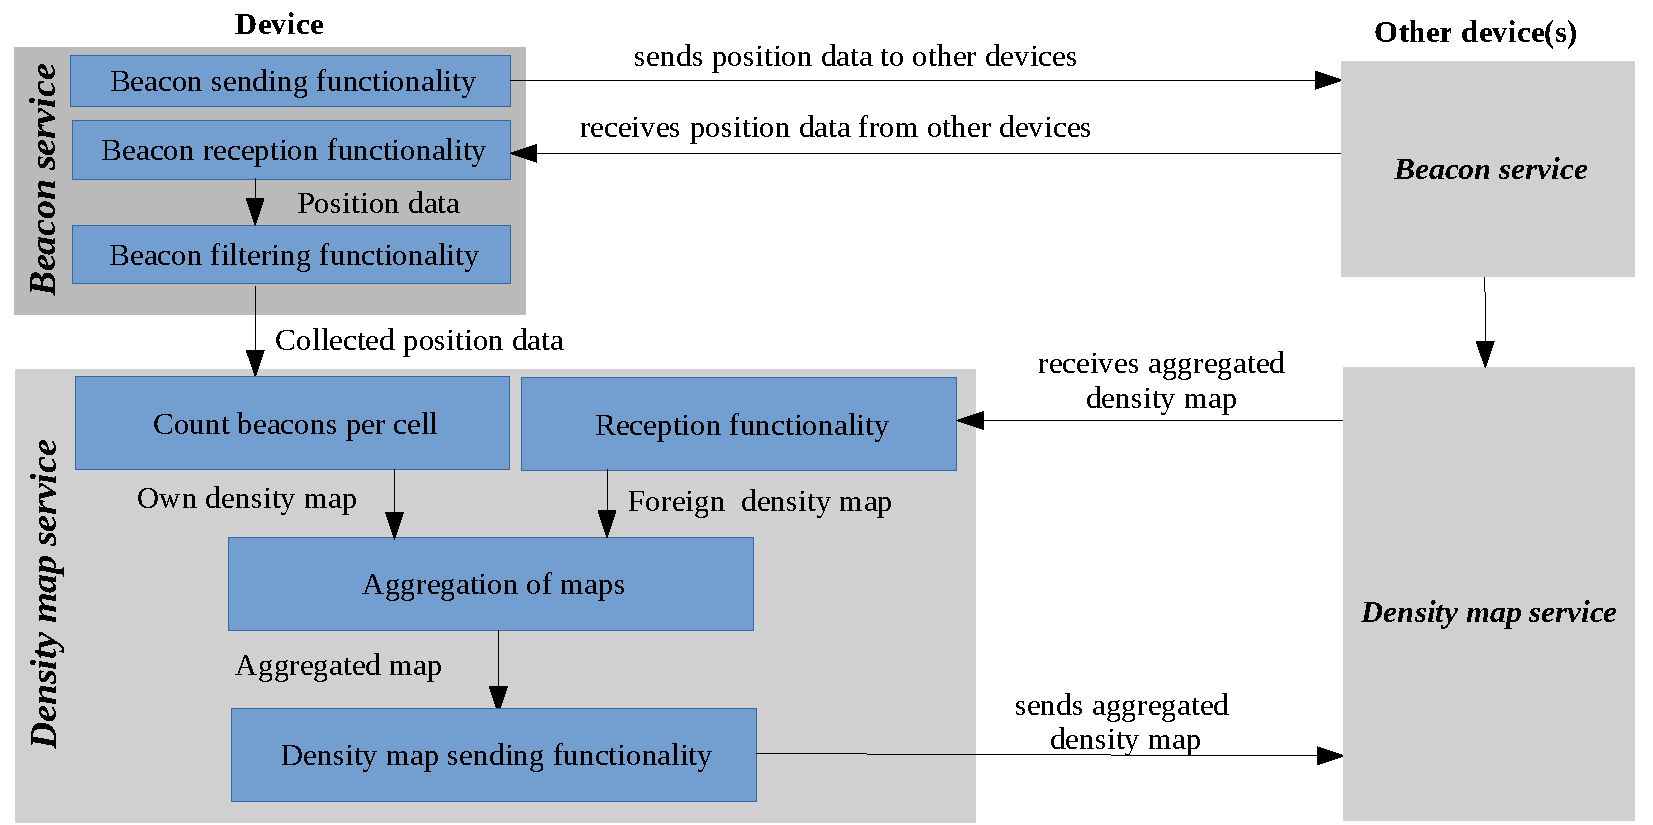
\includegraphics[width=\textwidth]{./crownet/services.pdf} 
\caption[Estimating the pedestrian density map: apps and services]{Overview of services of the density map application~\cite{schuhbaeck-2023-com}. Beacons and density maps are shared between devices using separate services. To improve the accuracy, density maps are aggregated.}
\label{fig:services-crowdsensoring}
\end{figure}

\begin{figure}
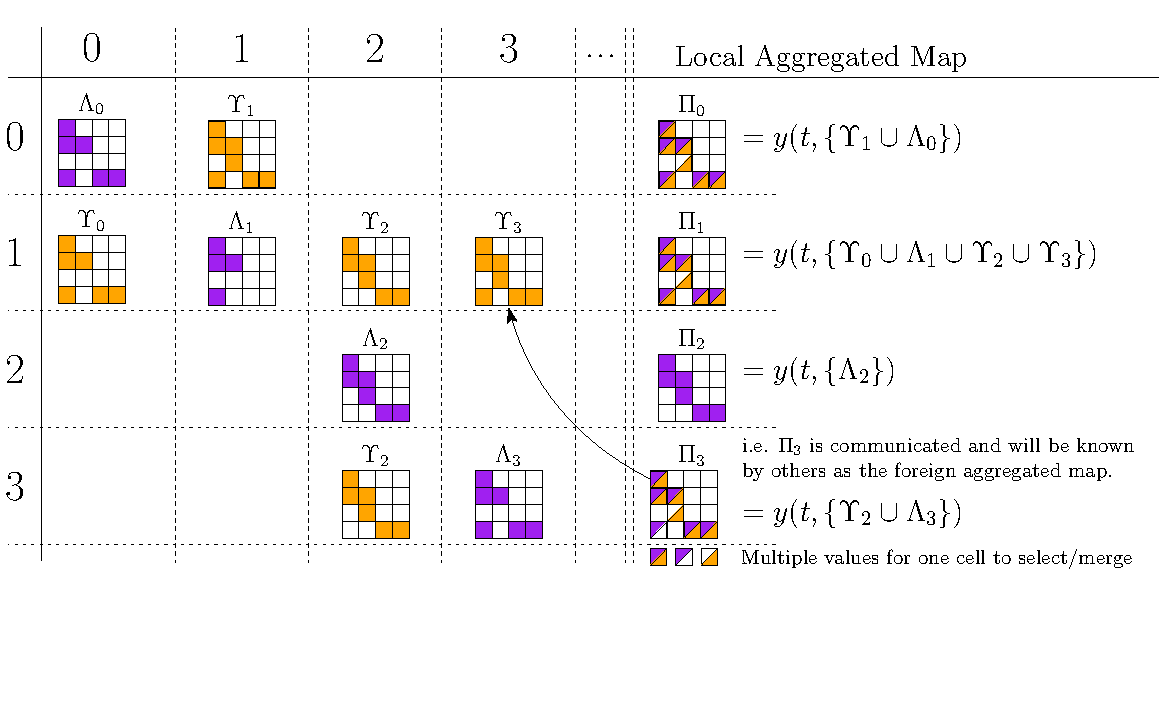
\includegraphics[width=\textwidth]{../figures/crownet/map_matrix.pdf} 
\caption{Availability of density information for the aggregation. If a matrix element contains a map, a device (row) has received density information from another device (column). The diagonal is always occupied, as each device counts beacons (own estimate). The matrix is not symmetric because some nodes have more reception range than others. Graphics from~\cite{schuhbaeck-2023-com}; permission granted by the creator S. Schuhbäck.}
\label{fig:aggregation}
\end{figure}


 

\subsection{Applications for disseminating route recommendations}

Two mobile applications were implemented in \textit{OMNeT++} to disseminate route information via direct communication. The first application is implemented in the C++-class \lstinline{UdpDetourAppVadere.cc}. It sends route recommendations at fixed intervals. The application is intended for simple crowd management applications where static detour information is sufficient and one can assume that people follow route recommendations. The recommended alternative route is changed directly in the crowd simulator by setting the target via the Traffic Control Interface, see Listing~\ref{lst:udpdetourapp}.

\begin{lstlisting}[float,floatplacement=hbt!,caption={\lstinline{actOnIncident()} method of the \lstinline{UdpDetourAppVadere} application. The application is intended for simple crowd management applications with static detour information. It is assumed that all pedestrians follow route recommendations: When a route recommendation is received, the target of the agent is directly changed over the Traffic Control interface.},language=C, label=lst:udpdetourapp]
void UdpDetourAppVadere::actOnIncident(
    IntrusivePtr<const DetourAppPacket> pkt) {
    
  ...
  std::string blocked = std::string(pkt->getClosedTarget());
  std::vector<std::string> targetLists = ctrl->getTargetList();
  if (std::find(targetLists.begin(), targetLists.end(), blocked) !=
      targetLists.end()) {
    std::vector<std::string> newTargetlist{};
    for (int i = 0; i < pkt->getAlternativeRouteArraySize(); i++) {
      newTargetlist.push_back(pkt->getAlternativeRoute(i));
    }
    ctrl->setTargetList(newTargetlist); // change target in Vadere over TraCI
  }
}
\end{lstlisting}

The second application enables the dissemination of dynamically generated route recommendations. As input, the app receives route recommendations provided by the \textit{flowcontrol} simulator via the Traffic Control Interface, see Fig.~\ref{fig:udpappcrownet}. The application is implemented in the \lstinline{BroadCastControlApp} application that is part of the compound module \lstinline{CrownetUdpApp}.
The \lstinline{ControlManager} class processes the input data.\textit{}
The scheduler of the \lstinline{CrownetUdpApp} schedules a packet that is immediately disseminated in the mobile network via the \lstinline{BroadCastControlApp}. The reception of route recommendations is implemented in the \lstinline{handleDataArrived()} method. As soon as a   route recommendation is received, it is forwarded to \textit{Vadere}, again using the Traffic Control Interface. Whether a node can send or receive route recommendations is configured through a boolean parameter.


\begin{figure}[hbt!]
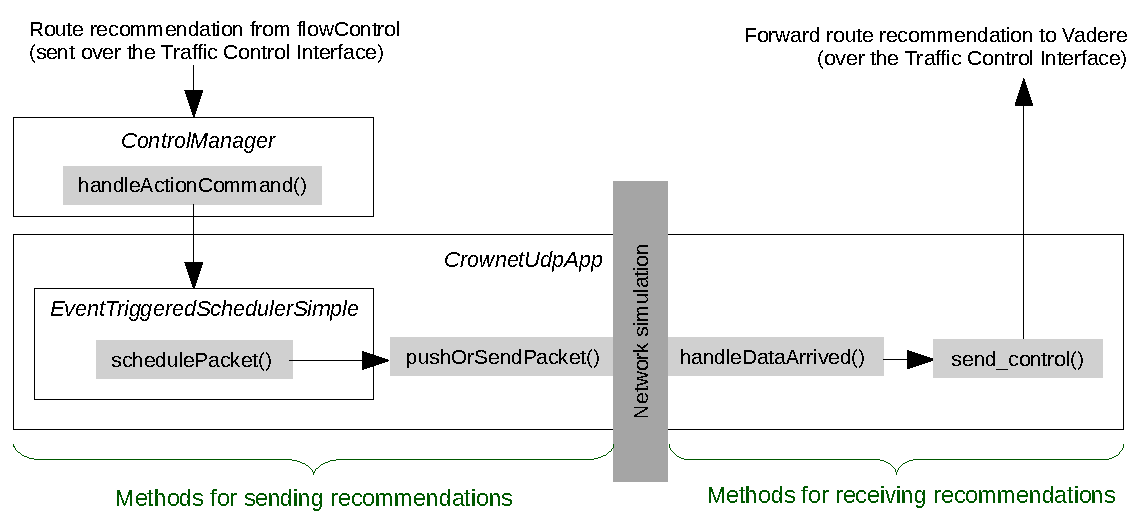
\includegraphics[width=\textwidth]{../figures/crownet/crownetapp.pdf} 
\caption{\lstinline{CrownetUdpApp} application and related classes. The class communicates via the Traffic Control Interface with the two simulators \textit{flowcontrol} and \textit{Vadere}. The \lstinline{CrownetUdpApp} has sending and receiving functionalities. The \lstinline{ControlManager} forwards route recommendations from the Traffic Control Interface to the \lstinline{CrownetUdpApp application} (left). Received route recommendations are forwarded to the \textit{Vadere} simulator (right). In the networks simulation the packet transmission is simulated.}
\label{fig:udpappcrownet}
\end{figure}




\section{Module Vadere: simulator extensions}

\label{sec:vadere}
The \textit{Vadere} simulator~\cite{kleinmeier-2019-cdyn} is used in \textit{CrowNet} to simulate crowd behavior. \textit{Vadere} has a psychology layer implemented which is essential for modeling  behavioral changes in a crowd guidance system. \textit{Vadere} contains several validated locomotion models, such as the Optimal Steps Model. To exchange data with other simulators, the Traffic Control Interface was implemented in~\cite{schuhbaeck-2019-com}. In the following I analyze the state-of-the-art simulator. Then I describe the adjustments that were necessary to integrate \textit{Vadere} in \textit{CrowNet}.


\subsection{State-of-the-Art simulator: analysis and required extensions}

\textit{Vadere} follows a model-view-controller software design pattern~\cite{kleinmeier-2019-cdyn}. The \lstinline{state} package (`model') contains the model classes that contain the state and the properties of objects, such as the size of an obstacle. The \lstinline{simulator} package (`controller') is responsible for the execution of the models. The \lstinline{gui} package (`view') contains \textit{Vadere}'s 2D graphical user interface. The core of \textit{Vadere} is the simulations loop, see Listing~\ref{lst:vadereloop}. At each simulation time step the layers of the psychology layer~\cite{kleinmeier-2021-cdyn} are executed sequentially. 
Stimuli are specified in \textit{Vadere}'s config file: the *.scenario file. It is not possible to generate stimuli dynamically and add them to the simulation online. 


\begin{lstlisting}[language=java, caption={Vadere simulation loop including psychology layer~\cite{kleinmeier-2020-cdyn}.},label=lst:vadereloop]
while (simulationIsRunning) {
  ...
  perceptionModel.update (agents, stimuli); // Perception
  cognitionModel.update(agents); // Cognition
  locomotionModel.update(agents,time); // Locomotion
  time ++;
  ...
}
\end{lstlisting}




For each time step, the \lstinline{StimulusController} extracts stimuli from the \lstinline{ScenarioStore} object.  Stimuli are always addressed to the entire population of agents. It is not possible to address stimuli to an individual agent. Therefore, it is not possible to simulate how an agent receives a mobile message.


At the perception layer the most important stimulus is selected which is then passed to the cognition layer where a self-category is selected in dependency of the most important stimulus and environmental conditions.  
Since each self-category is assigned exactly one specific behavior to keep it simple as simple as possible~\cite[p.95]{kleinmeier-2021-cdyn}, one cannot simulate that people show different behaviors. In a crowd guidance system, some people follow the route recommendations and some others do not. Therefore, adjustments are necessary.

Parameters of the psychological models are hard-coded. Parameter studies are, therefore, only possible by changing the source code. Systematic uncertainty quantification is not possible.


I conclude that the state-of-the-art \textit{Vadere} simulator (release 1.6, 2022) needs to be adapted. I derive the following requirements, see Tab~\ref{tab:requirementsvadere}.

\begin{table}[hbt!]
\begin{tabular}{|p{8cm}|p{6cm}|}
\hline
\textbf{Requirement} & \textbf{Design decision}  \\
\hline 
 Uncertainty quantification must be possible for psychological models.
  & Parametrize the psychology layer (see Section~\ref{sec:Parametrizationofthepsychologylayer}). \\ \hline 
 It must be possible to model and simulate the effect that agents respond differently to the same information. & Extend the functionalities of the psychology layer (see Section~\ref{sec:Enablingbah}).\\ \hline 
 The reception of individual stimuli (mobile messages) must be possible. & Generalize the stimulus definition and processing (see Section \ref{sec:generalizestimulus}). \\
 \hline 
%Data exchange  with other simulators is necessary. & Implement the Traffic Control Interface \\ 
\end{tabular} 
\caption[Requirements on the extension of the \textit{Vadere} simulator.]{Required extensions for the \textit{Vadere} simulator release 1.16. To use \textit{Vadere} as mobility provider in a crowd guidance system several adjustments are necessary. The design decisions (right) describe how the required adjustments (left) are implemented. }
\label{tab:requirementsvadere}
\end{table}



\subsection{Parametrization of the psychology layer}
\label{sec:Parametrizationofthepsychologylayer}

To enable parameter studies with psychological models, \textit{Vadere}'s psychology layer is parameterized. For this purpose, I introduce attribute classes for the models of the perception layer and the cognition layer. Each model class is assigned a unique attribute class. If the scenario is set up using the \lstinline{VadereGui}, the corresponding attribute class is automatically inserted. Each attribute class has a corresponding \lstinline{json} counterpart so that parameter values can be specified in the scenario file. 


Listing~\ref{lst:jsonpsychologynew} shows an example how a psychological model can be parameterized over the *.scenario file. The parameter values of the \lstinline{ProbabilisticCognitionModel} are defined in the respective attribute class. The idea of the model is that agents take a route with a certain probability when they receive a route recommendation. The route probabilities are specified as vector, see \lstinline{targetProbabilities} in Listing~\ref{lst:jsonpsychologynew}.  Tests ensure that the sum of probabilities equals 1. 




\subsection{Enabling behavioral repertoires}
\label{sec:Enablingbah}

In reality, people react differently even with the same environmental information due to their individual experiences and daily behavior. To allow different behaviors, the cognition layer is extended by the abstract class \lstinline{AProbabilisticModel}, see Fig.~\ref{fig:probabilisticmodels}. 

\begin{lstlisting}[caption={Parameterization of psychological models in Vadere's scenario file. The \lstinline{targetProbabilities} parameter is a vector of probabilities. Each probability is assigned to a certain target (\lstinline{targetIds}). If the long route is recommended (\lstinline{instruction}), 25\% of the agents take target 11, 25\% take target 21. The majority (50\%) takes the long route (target 31).},language=Java,label=lst:jsonpsychologynew]
"attributesPsychology" : {
    "psychologyLayer" : {
        "perception" : "SimplePerceptionModel",
        "cognition" : "ProbabilisticCognitionModel",
        "attributesModel" : {
          " org.vadere.%.perception.AttributesSimplePerceptionModel" : {
            "priority" : { // control priority (assign integers: 1, 2, 3)
              "1" : "Threat",
              "2" : "Wait",
              "3" : "Information", 
            }},
          "org.vadere.%.cognition.AttributesProbabilisticCognitionModel" : {
            "routeChoices" : [ {
              "instruction" : "Please take the long route (id=31)",
              "targetIds" : [ 11, 21, 31 ],
                             // control route probabilites
              "targetProbabilities" : [ 0.25, 0.25, 0.50 ] 
            } ], ...
\end{lstlisting}

\begin{figure}[hbt!]
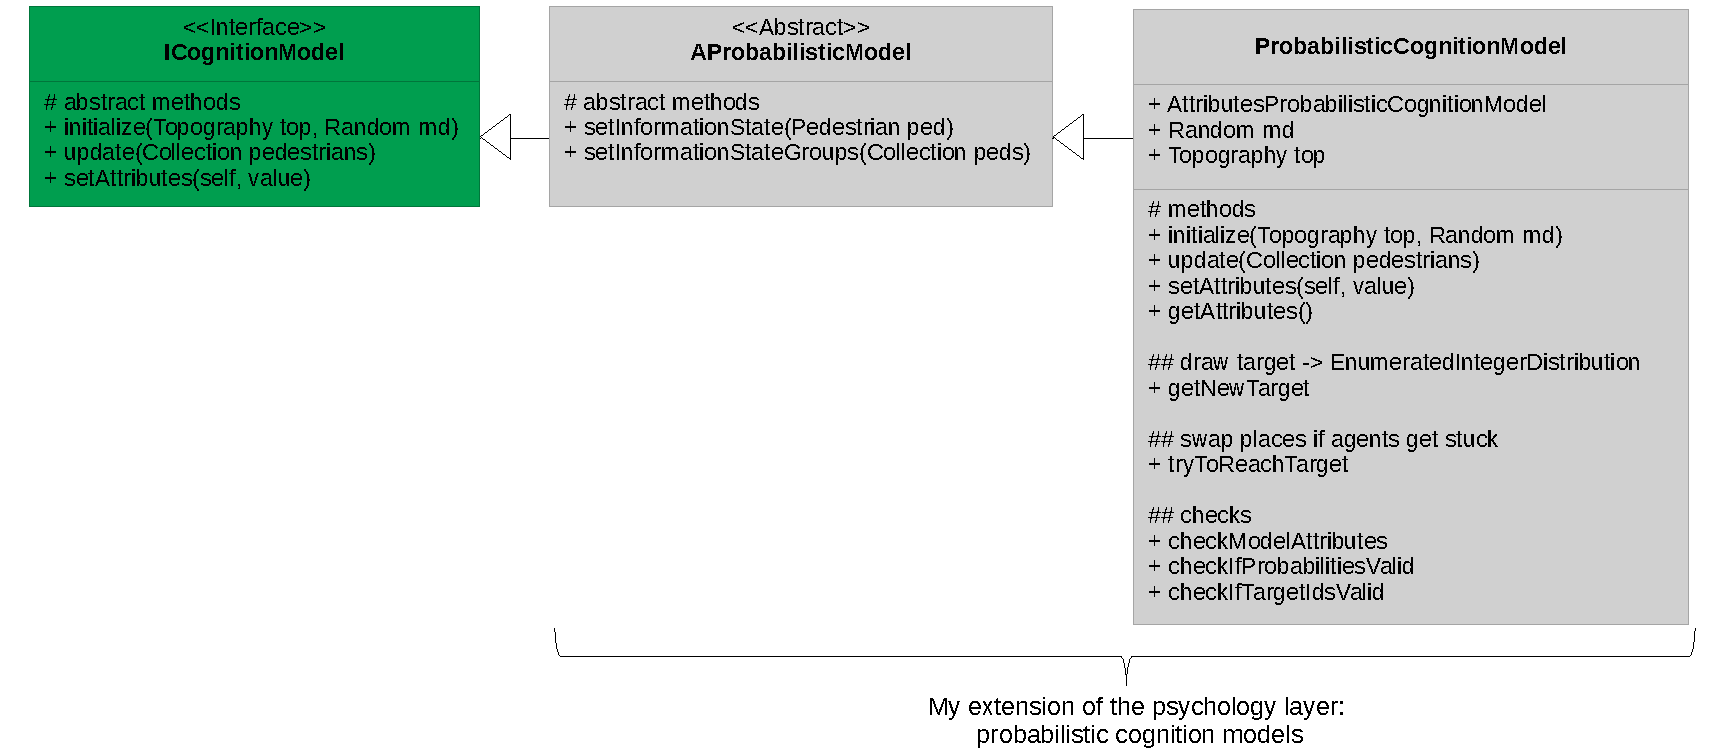
\includegraphics[width=1.05\textwidth]{./crownet/vadere_implementation_new_models.pdf} 
\caption[Introducing probabilistic models in \textit{Vadere}'s CognitionLayer]{Extending  \textit{Vadere}'s cognition layer. The abstract class \lstinline{ProbalisticModel} is added to enable probabilistic choice modeling.}
\label{fig:probabilisticmodels}
\end{figure}


Instead of deriving the self-category from the most important stimulus, the self-category is determined probabilistically: For each behavior a certain probability is assigned. An example is the \lstinline{ProbabilisticCognitionModel}, see again Listing~\ref{lst:jsonpsychologynew}. It models the route choice behavior probabilistically. The routes 11 and 21 are taken with a probability of 25\,\% each and route 31 with a probability of 50\,\%. 

For any probabilistic model, it is assumed that an agent makes a decision only when new information comes in. The decision-making is realized by drawing from a random distribution. If the same information is received again, it is ignored because it has been already processed. To achieve this, the information state of an agent must be stored. 
I introduce the \lstinline{InformationState} that is an \lstinline{enum} with the values \lstinline{NO_INFORMATION, INFORMATION_RECEIVED}, \lstinline{INFORMATION_CONVINCING_RECEIVED, INFORMATION_UNCONVINCING_RECEIVED}. Another enum item is \lstinline{FOLLOW_INFORMED_GROUP_MEMBER} that is intended for group members who make decisions together. 
To display the \lstinline{InformationState}, the GUI is extended. 





\subsection{Generalization of the stimulus definition and processing}
\label{sec:generalizestimulus}

The \lstinline{SimulationCommandHandler} is introduced to add route recommendation stimuli dynamically to the simulation. The class handles \lstinline{StimulusInfo} objects that are received over the Traffic Control Interface. It extracts the \lstinline{StimulusInfo} object from the bit stream and adds the object to the \lstinline{StimulusInfoStore}. Therefore, \lstinline{StimulusInfoStore} contains static stimuli from the *.scenario file and dynamically received stimuli, see Fig.~\ref{fig:processingstimuli}. 



\begin{figure}[hbt!]
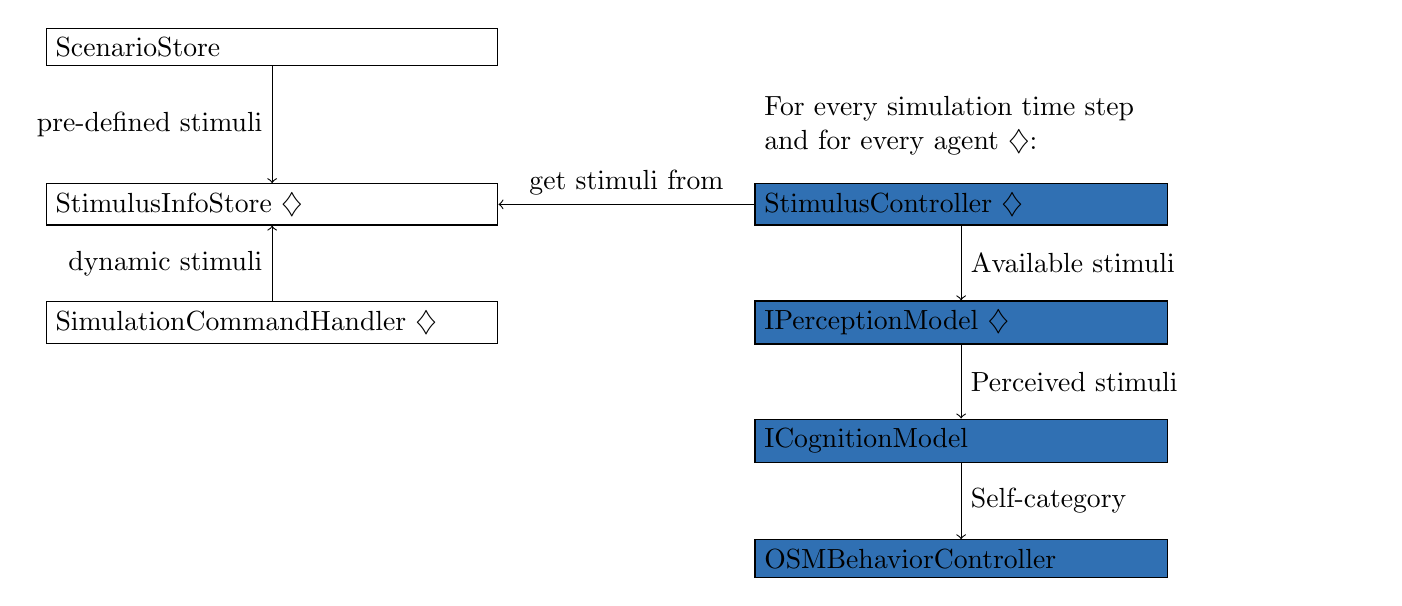
\begin{tikzpicture}
 \node[anchor=west,rectangle,draw,text width=5.5cm] (scenariostore) at (-1,3.5) {ScenarioStore};
  \node[anchor=west,rectangle,draw,text width=5.5cm] (commandhandler) at (-1,0) {SimulationCommandHandler $\diamondsuit$};
 \node[anchor=west,rectangle,draw,text width=5.5cm] (ss) at (-1,1.5) {StimulusInfoStore $\diamondsuit$};
 \node[anchor=west, text width= 5.0cm] (sc) at (8,2.5) {For every simulation time step and for every agent $\diamondsuit$:};
 \node[anchor=west,rectangle,draw,text width=5.0cm,fill=blue] (sc) at (8,1.5) {StimulusController $\diamondsuit$};
 \node[anchor=west,rectangle,draw,fill=blue,text width=5.0cm] (ip) at (8,0) {IPerceptionModel $\diamondsuit$};
 \node[anchor=west,rectangle,draw,fill=blue,text width=5.0cm] (ic) at (8,-1.5) {ICognitionModel};
 \node[rectangle,draw,anchor=west,fill=blue,text width=5.0cm] (osm) at (8,-3) {OSMBehaviorController};
 \draw[<-](ss) -- (sc) node[midway,above] {get stimuli from};
 \draw[->](sc) -- (ip) node[midway,right] {Available stimuli};
  \draw[->](ip) -- (ic) node[midway,right, text width=5.0cm] {Perceived stimuli};
   \draw[->](ic) -- (osm) node[midway,right,text width=5.0cm] {Self-category };
 \draw[->](scenariostore) -- (ss) node[midway,left] {pre-defined stimuli};
  \draw[->](commandhandler) -- (ss) node[midway,left] {dynamic stimuli};

\end{tikzpicture}
\caption[Processing dynamic stimuli in Vadere]{Processing dynamic stimuli in \textit{Vadere}. Novel or adjusted classes are marked with $\diamondsuit$. Stimuli are dynamically received over the Traffic Control Interface implemented in~\cite{schuhbaeck-2019-com}.
The adjusted \lstinline{SimulationCommandHandler} adds the stimuli to the \lstinline{StimulusInfoStore}. Since agents receive route recommendations at different times, it is necessary to address stimuli to specific agents. To achieve this, the filtering functionalities of the \lstinline{StimulusController} are extended. Also, the \lstinline{update} method of the \lstinline{IPerceptionModel} is adjusted to enable the processing of agents-specific stimuli.  }
\label{fig:processingstimuli}
\end{figure}

Due to delays, pedestrians may receive route recommendations at different times via their mobile applications. Therefore, it is mandatory that a route recommendation stimulus can be addressed to an individual agent. To achieve this, a \lstinline{SubpopulationFilter} is added to the existing \lstinline{StimulusInfo} class. The \lstinline{SubpopulationFilter} has a list attribute that contains agents ids. For agents in the list, the stimulus is forwarded to the perception layer.

Route recommendations should be only displayed in areas where they are actually needed. In real life, the mobile application would check whether information should be displayed. In the simulation, this functionality is provided by a novel spatial filter: The \lstinline{Location} attribute ensures that a stimulus is only generated for agents in a certain area. If the agent is in a certain area, the stimulus if forwarded to the perception layer.

The \lstinline{SubpopulationFilter} and the \lstinline{Location} are added to the \lstinline{StimulusInfo} as attributes. The extended class has four attributes:

\begin{itemize}
\item \lstinline{stimuli} of type \lstinline{List<Stimulus>}: route recommendations, waiting signals, bangs, ... (unchanged)
\item \lstinline{timeframe} of type \lstinline{Timeframe}: defines the time slot in which stimuli are active (unchanged)
\item \lstinline{location} of type \lstinline{Location}: defines the spatial area in which stimuli are active (novel attribute)
\item \lstinline{subpopulationFilter} of type \lstinline{SubpopulationFilter}: defines which agents have access to the stimuli (novel attribute)
\end{itemize}



The objects \lstinline{timeframe, location} and \lstinline{subpopulationFilter} are employed for filtering stimuli for space and time and address them to specific agents. The \lstinline{StimulusController} and the interface \lstinline{IPerceptionModel} are adjusted for this purpose. The filtering functionalities of the \lstinline{StimulusController} are extended to allow spatial and agent-specific filtering. Note that the original implementation only supported a time-based filtering. 

Because the provision  and the perception of a stimulus are two separate processes, I introduce two stages:
\begin{itemize}
\item First the availability of a stimulus is checked by the \lstinline{StimulusController}: Has the mobile device received a route recommendation and is this route recommendation displayed to the virtual pedestrian?
\item Second the perception is modeled at the perception layer: How is the message perceived? Are there any other stimuli?
\end{itemize}
The separation of concerns is achieved by adjusting the \lstinline{update} method of the \lstinline{IPerceptionModel} interface. Instead of using a list that contains stimuli perceived by the entire population, a map is used. Each agent has an individual list of available stimuli assigned: \lstinline{void update(HashMap<Pedestrian, List<Stimulus>> pedSpecificStimuli);}. 




\section{Module flowcontrol: novel framework for route recommendation algorithms}
\label{sec:flowcontrol}


\subsection{Scope, software architecture and requirements}
\textit{flowcontrol} is a novel Python simulation framework that I developed as part of this thesis. It is my major contribution to the \textit{CrowNet} simulation framework. The scope of \textit{flowcontrol} is to provide algorithm that generate route recommendations for crowd models.
In \textit{CrowNet}, \textit{flowcontro}l is used in combination with the \textit{Vadere} simulator. 
%
\textit{flowcontrol} has a modular architecture and follows a model view controller pattern, see Fig.~\ref{fig:mvcflow}. 


\begin{figure}[hbt!]
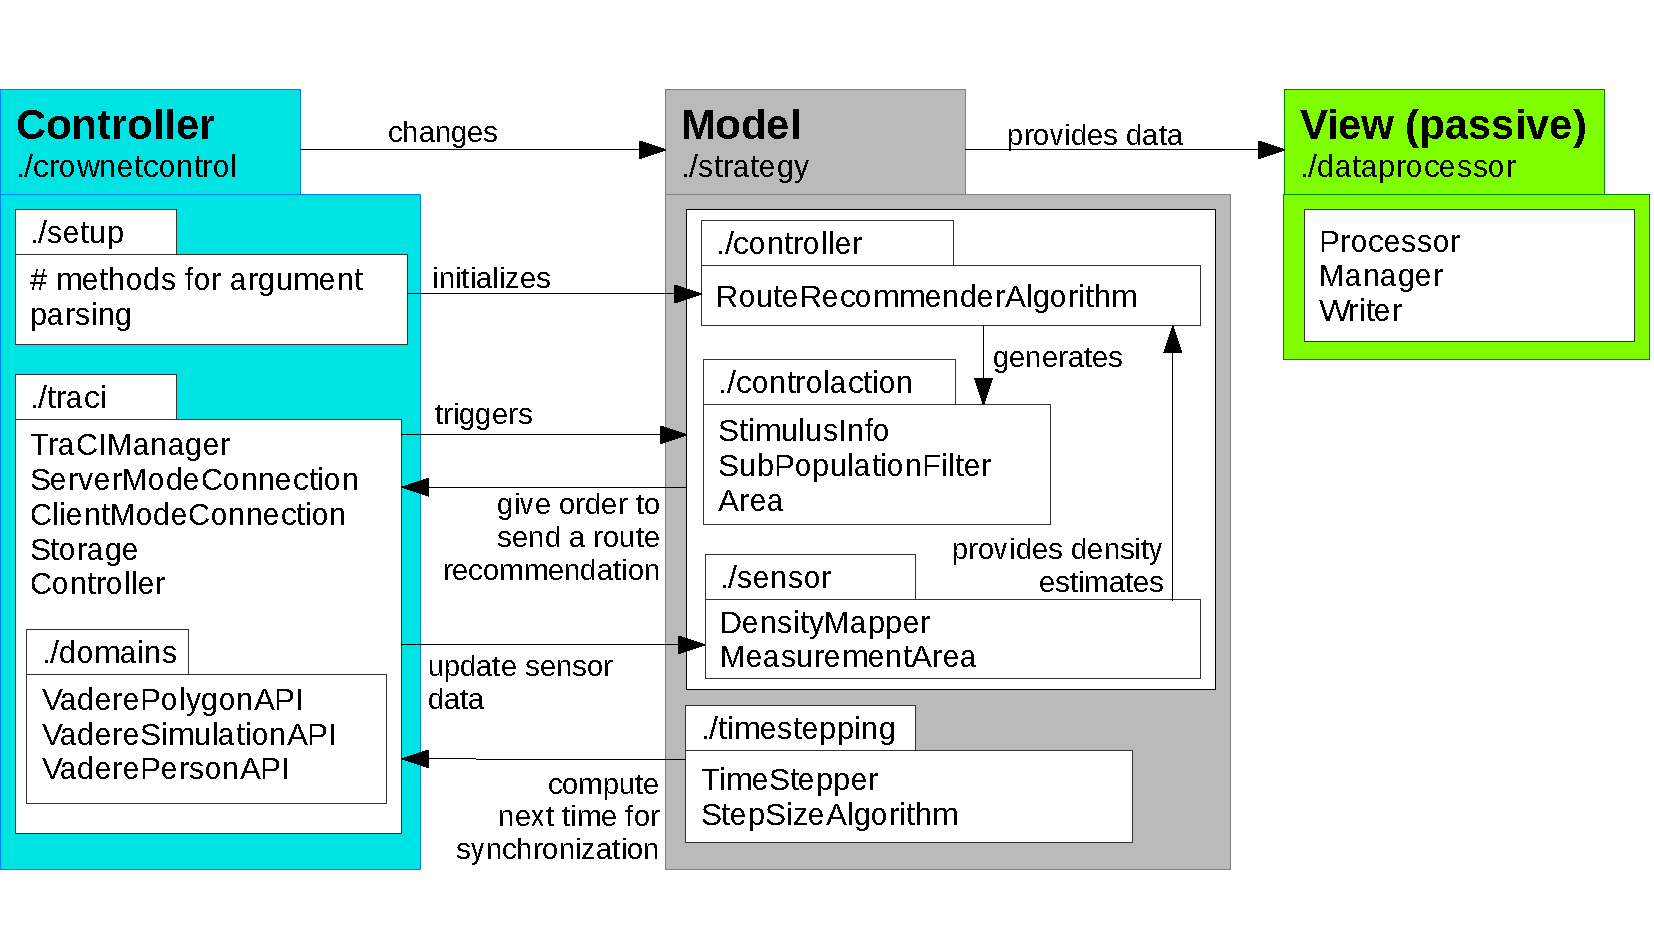
\includegraphics[width=\textwidth]{./crownet/flowcontrol_MVC.pdf} 
\caption[flowcontrol: packages and important classes of the Python  framework ]{Architecture of the novel simulation framework \textit{flowcontrol}. The scope of \textit{flowcontrol} is to provide route recommendations for pedestrian dynamics simulators, such as \textit{Vadere}.  Route recommendation algorithms, time stepping procedures and methods for mapping sensor data are implemented in the \lstinline{strategy} package (`Model'). The data exchange with other simulators is handled in \lstinline{crownetcontrol/traci} (`Controller'). \textit{flowcontrol} uses the graphical user interface of the crowd simulator: The \lstinline{dataprocessor} package (`View') provides additional data processors. }
\label{fig:mvcflow}
\end{figure}


The \lstinline{strategy} package (`Model') contains the core elements for generating route recommendations. It contains several sub-packages, see again Fig.~\ref{fig:mvcflow}. 
The \lstinline{controller} sub-package contains the route recommendation algorithms. The \lstinline{timestepping} sub-package contains methods to control the time between two route recommendations. The sub-package \lstinline{controlaction} provides representations for route recommendations. For example, the \textit{Vadere} simulator requires that a route recommendation is a \lstinline{StimulusInfo} object in JSON format. To couple \textit{flowcontrol} with another pedestrian dynamics simulator, one simply implements the simulator-specific representation of a route recommendation.


The package \lstinline{crownetcontrol/traci} (`Controller') manages the transfer of route recommendations over the Traffic Control Interface. If the complete crowd guidance system should be simulated, the recommendation is sent to \textit{OMNeT++}. \textit{OMNeT++} simulates the transmission of the route recommendation in the mobile network. When the packet is received, the route recommendation is forwarded to \textit{Vadere}. When the network simulation is not needed, \textit{flowcontrol} sends the route recommendation directly to \textit{Vadere}. Depending on the simulator combination, \textit{flowcontrol} is either the client or the server, see again Fig.~\ref{fig:configurationCrownet} in Section~\ref{sec:crownetutils}. 

 
As most pedestrian simulators \textit{Vadere} provides a graphical user interface and visualization tools which is why \textit{flowcontrol} does not provide a user interface. The processors and export functionalities in the  \lstinline{dataprocessor} package (`View') only serve to verify the results. 

For the development of \textit{flowcontrol}, I adhere to the principles of software development: I use code quality measures (see Section~\ref{sec:requirementglobal}) and define requirements, see Tab.~\ref{tab:requirementsflowcontrol}. \textit{flowcontro}l has an own continuous integration pipeline that is triggered with every commit. Unit tests verify the correct implementation of methods. Integration tests ensure that the simulator coupling works.




\begin{table}[hbt!]
\begin{tabular}{|p{7cm}|p{7cm}|}
\hline
\textbf{Requirement} & \textbf{Design decisions}  \\
\hline 
Route recommendation algorithms for crowds must be provided that can be transferred to arbitrary scenarios; adding algorithms should be easy. & Provide algorithms that can be transferred to arbitrary scenarios; establish a reusable software structure by using suitable interfaces and a strategy pattern (see Section~\ref{sec:routerecommendationalgorithms}).  \\ \hline
 It must be possible to control the time between two evaluations of the route recommendation algorithm (time interval). & Separate the time stepping procedure from the logic of the algorithm and provide time stepping procedures (see Section~\ref{sec:timestepping}). \\ \hline
It should be possible to use density information from the decentralized density maps application (Section~\ref{sec:novelapplication}) as input for the route recommendation algorithm. & Implement a procedure that extracts the necessary density information from the application data (see Section~\ref{sec:mappingproc}).  \\
\hline
\end{tabular} 
\caption[Requirements on the novel flowcontrol simulator.]{Main requirements for the novel \textit{flowcontrol} simulator. The design decisions (right) describe how the requirements for the simulator (left) are implemented.  }
\label{tab:requirementsflowcontrol}
\end{table}




\FloatBarrier


\subsection{Route recommendation algorithms: the logic of guidance}
\label{sec:routerecommendationalgorithms}
The redirection logic of the route recommendation algorithm is implemented in the \lstinline{strategy} module. To enable developers to easily extend the simulation framework, a strategy software design pattern is used. With this, new algorithms can be simply added by inheriting from the abstract class \lstinline{RouteRecommendationAlgorithm}, see Fig.~\ref{fig:routerecommalg}. 
The static helper method \lstinline{get_controller_from_args} creates and initializes an object of the type \lstinline{RouteRecommendationAlgorithm} defined in \lstinline{run_script.py} (\lstinline{--ctrl.controller-type}). The separation of algorithm logic and object initialization allows to extend the package easily which increases the re-usability and sustainability of the software. 


As I have outlined in the state of the art, several algorithms have been proposed for guiding crowds (see Section~\ref{sec:modelalg}). However, these are neither transferable to arbitrary scenarios, nor have they been tested under realistic conditions. Therefore I develop algorithms myself and implement them in the \lstinline{strategy} package. 

I suggest and implement the following algorithms:
\begin{itemize}
\item \lstinline{AlternateTargerAlgorithm}: alternates the routes sequentially.
\item \lstinline{AvoidCongestionAlgoritm}: recommends an alternative route whenever the density on the direct route is higher than on the alternative route.
\item \lstinline{MinimalDensityAlgorithm}: recommends the route where the density is the lowest. If there are only two routes, the algorithm is identical to \lstinline{AvoidCongestionAlgorithm}.
\end{itemize}


\begin{figure}[hbt!]
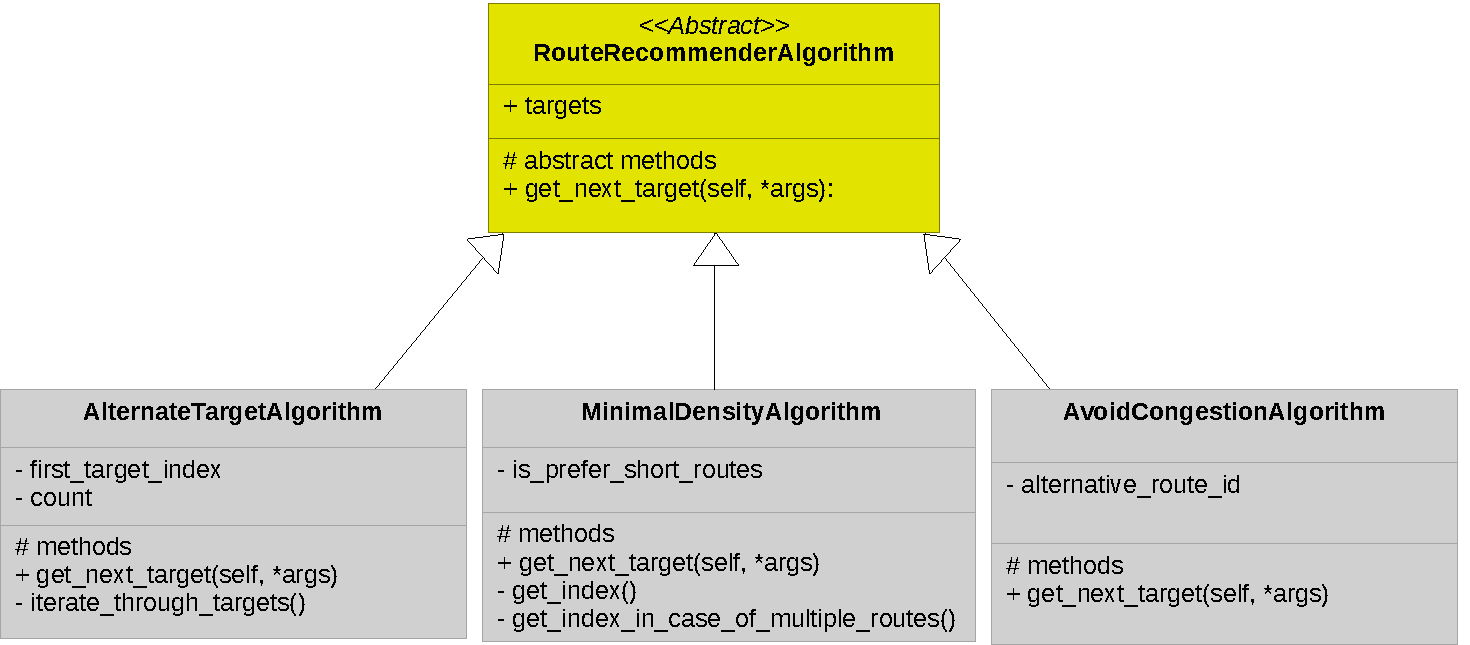
\includegraphics[width=\textwidth]{./crownet/flowcontrol_UML_guiding_strategy.pdf} 
\caption{Important classes for the implementation of route recommendation algorithms in the \lstinline{strategy} module. The core of the module is the abstract class \lstinline{RouteRecommendationAlgorithm}. The logic of a route recommendation algorithm is implemented in the \lstinline{get_next_target()} method of the respective child class.  }
\label{fig:routerecommalg}
\end{figure}



\subsection{Time stepping procedure }

\label{sec:timestepping} 

A core functionality of a dynamic crowd guidance system is the scheduling of route recommendations. In \textit{flowcontrol} this functionality is implemented in the \lstinline{timestepping} module. \textit{flowcontrol} offers different types of time stepping procedures that trigger the generation of route recommendation at regular or irregular time intervals, see Fig.~\ref{fig:timestepper}. 




\begin{figure}[hbt!]
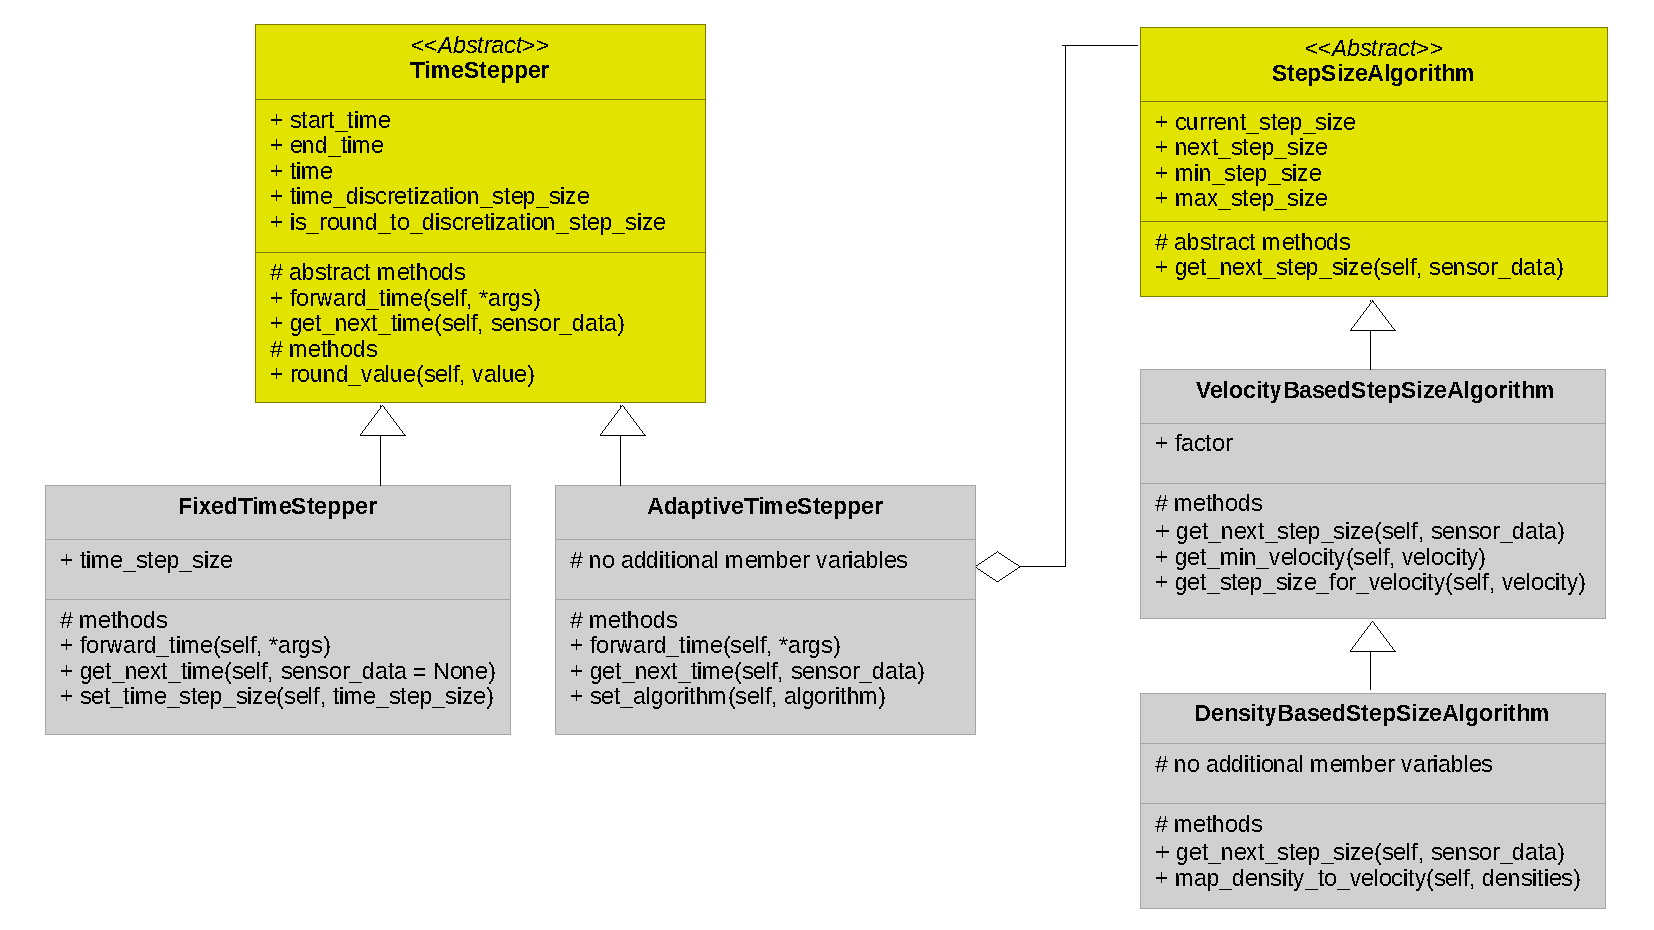
\includegraphics[width=\textwidth]{./crownet/flowcontrol_UML_timestepping.pdf} 
\caption[flowcontrol: Implementation of the time stepping]{
Time stepping procedure. The abstract class \lstinline{TimeStepper} controls the time in between two route recommendations. The time interval can be either fixed (\lstinline{FixedTimeStepper}) or dynamically adjusted during the simulation (\lstinline{AdaptiveTimeStepper}). For the latter, a \lstinline{StepSizeAlgorithm} is required that computes when the route recommendation algorithm should be evaluated next. }
\label{fig:timestepper}
\end{figure}

With a static stepping procedure, the time between two route recommendations is always the same. A dynamic stepping procedure adjusts the time between two route recommendations dynamically. A dynamic adjustment may help to reduce the number of redirection measures. This might be particularly helpful when the number of pedestrians changes dynamically over time: At a low arrival rate few redirection measures may be needed (large time interval) to dissolve congestion. At a high arrival rate (small time interval), pedestrians may need to be redirected more often. Therefore, the \lstinline{StepSizeAlgorithm} interface is introduced. Its core method is the abstract method \lstinline{get_next_time_step_size()} that has to be implemented by the child classes. 

\subsection{Extracting density information from density maps}
\label{sec:mappingproc}

Some route recommendation algorithms require density measurements. Densities are measured in areas where the maximum densities occur. I want to measure densities based on direct communication technology which is why I propose to use the decentralized density map application~\cite{schuhbaeck-2023-com}. However, a measurement area does not always correspond to a specific cell of the map, see Fig.~\ref{fig:mappingproblem}. 


\begin{figure}[H]
\centering
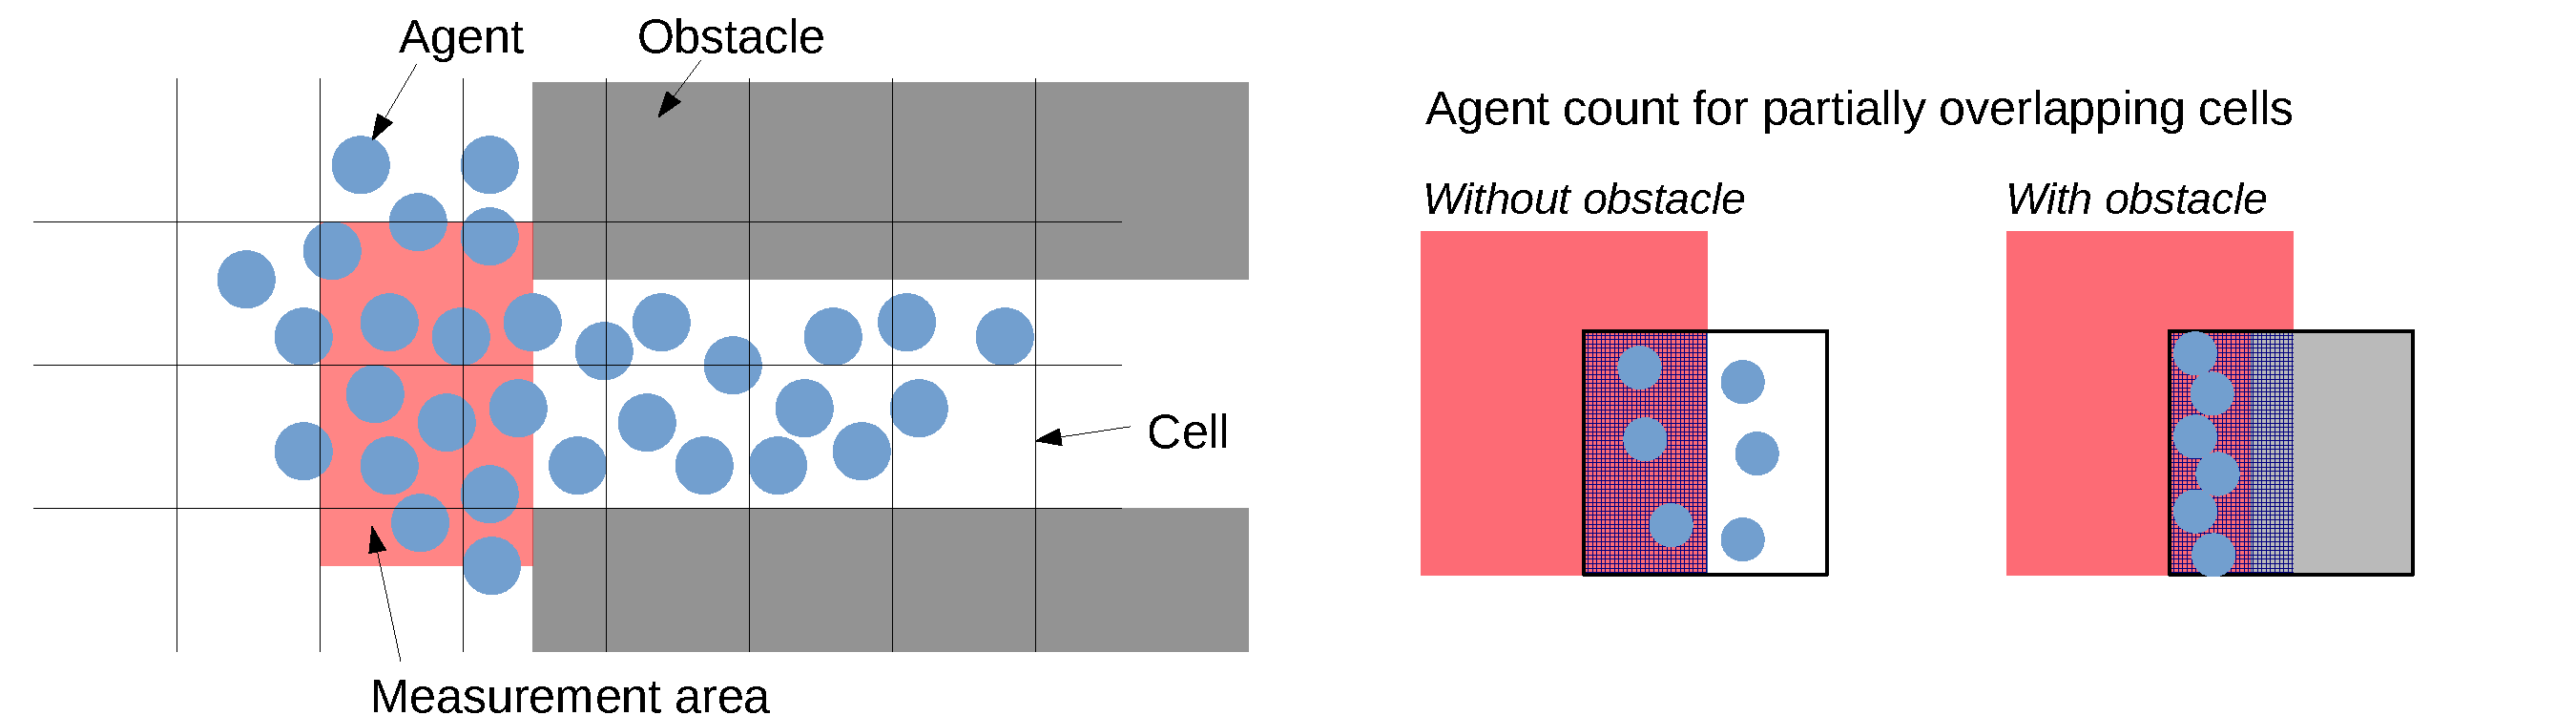
\includegraphics[width=0.9\textwidth]{./crownet/mappingalg.pdf} 
\caption[]{Mapping of density data. Since the measurement area is does not correspond to one cell of the density map application~\cite{schuhbaeck-2023-com}, a mapping is required. If obstacles cover parts of the cell, the reference area is small which leads to high densities (right). }
\label{fig:mappingproblem}
\end{figure}


The \lstinline{sensor} package provides a mapping procedure that computes the average density from cell-based data. The averaging procedure is implemented in the \lstinline{DensityMapper} that has information about the cell layout, the measurement areas and the obstacles, see Fig.~\ref{fig:densitymap}.  Since the density map application does not consider obstacles, densities could be locally underestimated which is not acceptable for crowd management applications. A simple correction procedure is implemented: The percentage of available space is determined for each cell. Then the density values are divided by the percentage values, given that a cell is not fully occupied by an obstacle.



\begin{figure}[H]
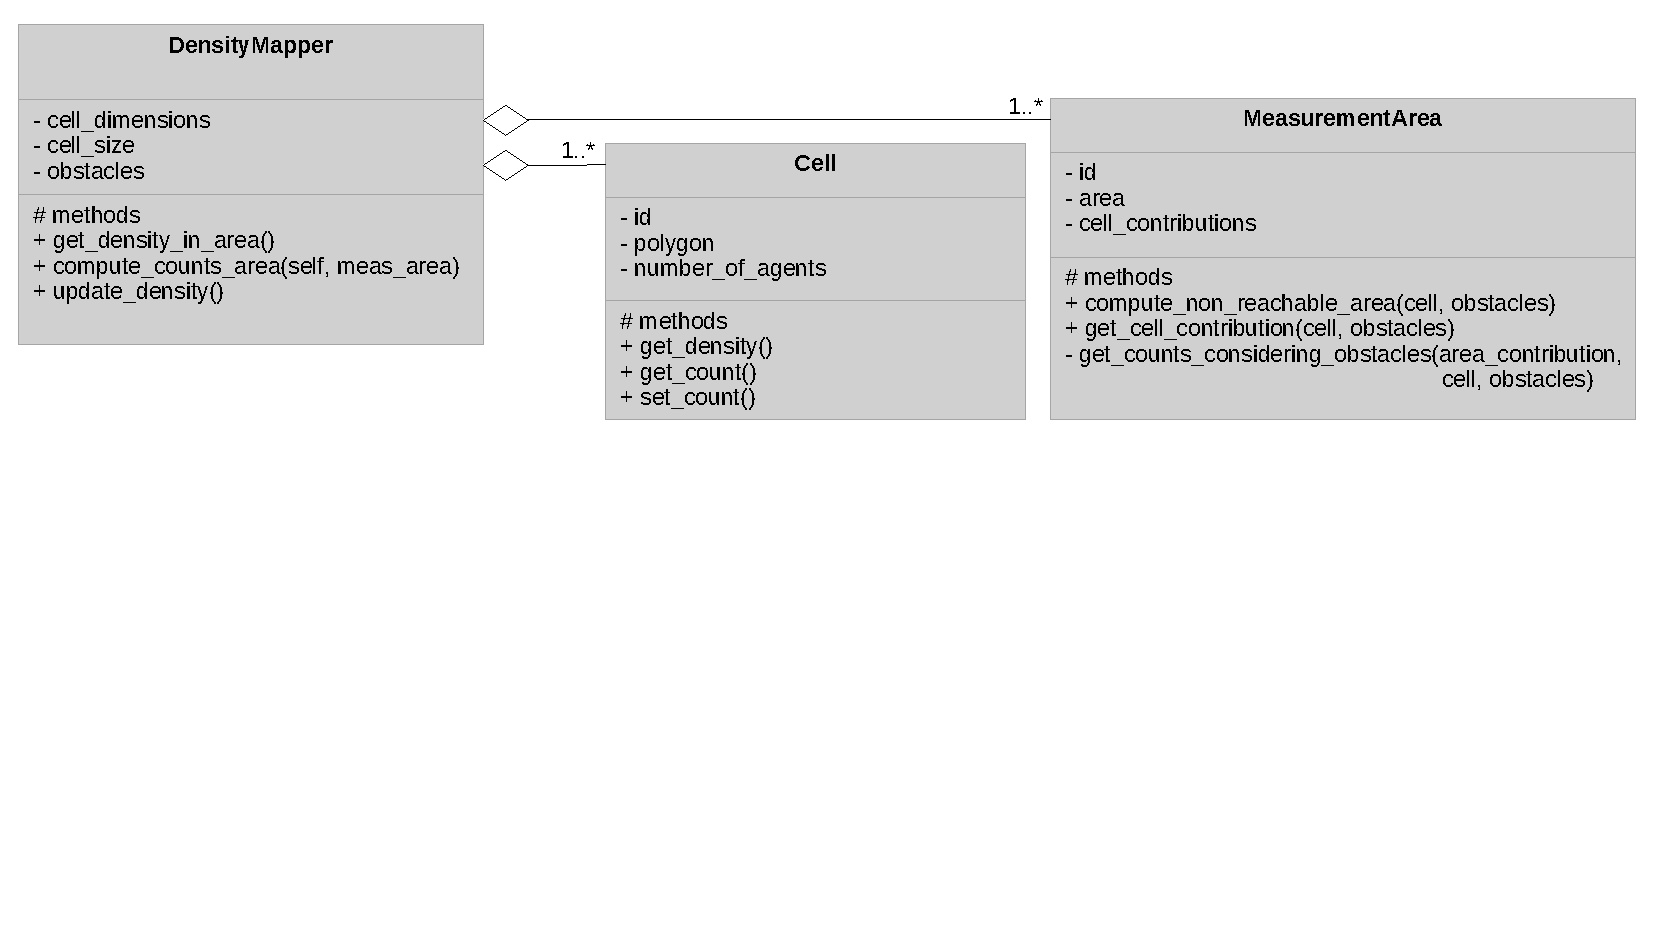
\includegraphics[width=\textwidth, trim=0.2cm 8.6cm 0.2cm 0.2cm, clip]{./crownet/flowcontrol_UML_sensor.pdf} 
\caption[Density estimation: implementation of a mapping approach ]{Important classes for the density estimation. The \lstinline{DensityMapper} has information about the measurement area (position, size) and the cell-grid (cell size, cell position). The \lstinline{DensityMapper}  estimates the crowd density in a measurement area from a density map~\cite{schuhbaeck-2023-com}.  }
\label{fig:densitymap}
\end{figure}










\section{Summary}

With \textit{CrowNet}, I created a new open-source framework to simulate a crowd guidance system where crowds are sensed and redirected using direct communication technology. First, I modeled a crowd guidance system composed of a crowd, a controller containing the route recommendation algorithm, a mobile application for sensing the crowd, and a mobile application for communicating route recommendations. Based on the model structure, I designed a modular software architecture. For the implementation, I defined functional and non-functional requirements and made design decisions to be realized in the corresponding modules. In addition, quality measures were defined to ensure software quality and sustainability. A continuous integration and deployment pipeline was introduced to test the source code during the development process. The core functionalities of the software were then implemented in the five main modules.

The \textit{crownetutils} module provides implementations for coupling models and simulators. An explicit update procedure was proposed and implemented, interpolating agent positions in the mobile communication simulation. To separate the inter-process communication of simulators from parallel executions and from the host system, the coupled simulation are executed in a containerized fashion, employing Docker networks. The state exchange between simulators is realized via the Traffic Control Interface. Several simulator couplings have been implemented for the simulation of the entire crowd system and for isolated subsystems. 

The \textit{SUQ-controller} enables to conduct parameter studies with coupled simulations. The module is based on the existing Python package \textit{SUQ-controller}. New process calls were added in order to be able to run coupled simulations. The definition of parameter combinations has also been extended. Parameters can now be changed in various simulator-specific config files. To ensure that only Docker containers communicate that refer to a specific parameter combination, a naming convention for the containers has been introduced.

The \textit{OMNeT++} module enables the simulation of direct communication. Existing simulators were employed as model libraries for the lower layers of the network. To sense crowds, a novel method based on LTE sidelink communication was implemented: the decentralized pedestrian density map application. Two further mobile applications were implemented to disseminate route recommendations, which differ in their static or dynamic information content.

The \textit{Vadere} module provides crowd models. The analysis of the state-of-the-art simulator showed that several extensions were required for the integration of \textit{Vadere} into \textit{CrowNet}: First, I generalized the stimulus definition and the processing of the stimuli in \textit{Vadere}'s psychology layer to enable dynamically generated route recommendations to be processed. Second, I introduced an interface for modeling probabilistic behavior in the cognition layer to enable probabilistic route choice. Third, I parameterized the psychology layer to permit parameter studies with behavioral models. With these extensions, route recommendations can be dynamically processed in \textit{Vadere}'s psychology layer. 

The module \textit{flowcontrol} has been developed for the provision of route recommendations. For this novel Python framework I first defined requirements from which I derived design decisions. Since state-of-the-art route recommendation algorithms did not fulfill my requirements, I proposed novel algorithms and implemented them. To control the time interval between two route recommendations, a generic time-stepping procedure has been implemented. To handle sensor data, a method was implemented that maps cell-based density values, provided by the density map application, to measurement areas. The \textit{flowcontrol} framework can be combined with other crowd simulators by implementing appropriate interfaces.


In the following chapter, I will use the \textit{CrowNet} software as a simulation tool to investigate my research question.

\chapter{Guiding crowds using direct communication technologies}
\label{sec:investigation}




In this chapter, I investigate how crowds can be redirected using direct communication technologies. For readers who are only interested in how I answer the main research question~(\hyperref[reserachquestions]{RQ}), I recommend to go directly to Section~\ref{sec:realistiscscenario}. If they have questions related to previous findings, that the study is based on, they can jump back. I answer my  research question following a step-by-step approach, see Fig.~\ref{fig:reserachdesign}. 


I first address my research sub-questions that relate to isolated components of my crowd guidance system. In Section~\ref{sec:infoverbreitung}, it is investigated how reliably route recommendations are disseminated using direct communication in a crowd (sub-question \hyperref[reserachquestions]{RQ-1}). I introduce a criterion to evaluate the reliability of information dissemination in a crowd and employ it in a simulation study.  In Section~\ref{sec:umleitalgorithmen}, the suitability of route recommendation algorithms is assessed under the condition that not all crowd members follow instructions~(sub-question \hyperref[reserachquestions]{RQ-2}). The effect of three heuristic algorithms on safety and comfort-related quantities, such as the level of service, is compared. From this study, I select the most suitable algorithm for my crowd guidance system. In Section~\ref{sec:reaction}, the third research sub-question~(\hyperref[reserachquestions]{RQ-3}) is investigated, that is,
how route recommendations should be designed in mobile messages so that crowd members follow instructions. 
The Sections~\ref{sec:infoverbreitung}-\ref{sec:reaction} are structured in the same way. First, the research scenario is presented, followed by the study design. Then, the results are discussed.  At the end of each section, a summary and a conclusion (`Lessons learned') are provided where I point out what the findings mean for the design of a crowd guidance system.

All the individual scenarios presented in Sections~\ref{sec:infoverbreitung}-\ref{sec:reaction} were inspired by an application scenario at the metro station Münchner Freiheit in Munich, Germany. Since I had to abstract and adapt the application scenario to create laboratory conditions to properly answer my research sub-questions, the scenarios differ in the plot, in the topography and in the resulting pedestrian streams. 
Readers who are interested in the application scenario,  find a detailed description in  Section~\ref{sec:reaction}.


In Section~\ref{sec:realistiscscenario}, I answer the main research question (\hyperref[reserachquestions]{RQ}). I propose and investigate a complete crowd guidance system. To test my concept, I assess the effect of the crowd guidance system for the application use case Münchner Freiheit (Munich, Germany), where footballs fans are guided from the bus to the train to resolve congestion. 



All simulation studies presented in this chapter were conducted with the \textit{CrowNet} software (Chapter~\ref{sec:crownet}). For the survey, ethical approval was obtained from the ethics committee of the Munich University of Applied Sciences, see Appendix~\ref{sec:ethicalapproval}.

\begin{tcolorbox}[float,floatplacement=hbt!,title=Availability of data]
Data presented in this chapter are publicly available, see Appendix~\ref{sec:availability}. This includes raw data and processed data.
\end{tcolorbox}



\begin{figure}[hbt!]
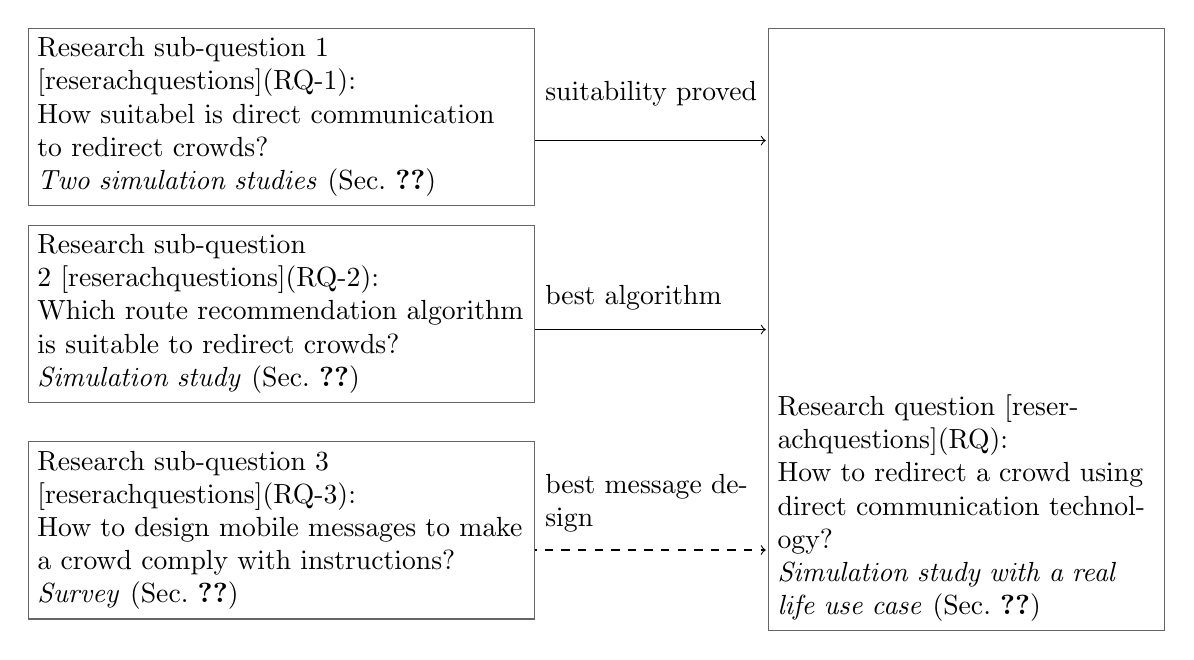
\begin{tikzpicture}
\draw [->] (3,-0.3) -- (6.65,-0.3);
\draw [->] (3,-2.7) -- (6.65,-2.7);
\draw [->, dashed] (3,-5.5) -- (6.65,-5.5);
\node[rectangle,draw=black!60,fill=white,text width=6.2cm] at (0.5,0.0)                            {{Research sub-question 1} ~\hyperref[reserachquestions]{(RQ-1)}: \\  How suitabel is direct communication to redirect crowds? \\ \textit{Two simulation studies}  (Sec.~\ref{sec:infoverbreitung})};
\node[rectangle,draw=black!60,fill=white,text width=6.2cm] at (0.5,-2.5)                            {{Research sub-question 2}~\hyperref[reserachquestions]{(RQ-2)}: \\ Which route recommendation algorithm is suitable to redirect crowds?\\ \textit{Simulation study}   (Sec.~\ref{sec:umleitalgorithmen})};
\node[rectangle,draw=black!60,fill=white,text width=6.2cm] at (0.5,-5.25)                            {{Research sub-question 3} ~\hyperref[reserachquestions]{(RQ-3)}: \\ How to design mobile messages to make a crowd comply with instructions? \\ \textit{Survey}  (Sec.~\ref{sec:reaction})};
\node[rectangle,draw=black!60,fill=white,text width=4.8cm, text height=4.8cm] at (9.2,-2.7)                            {Research question~\hyperref[reserachquestions]{(RQ)}: \\ How to redirect a crowd using direct communication technology? \\ \textit{Simulation study with a real life use case}  (Sec.~\ref{sec:realistiscscenario})};
%\draw [black,
    decorate, 
    decoration = {brace,
        raise=-15pt,
        amplitude=5pt}] (8,-4.5) --  (4,-4.5)
node[pos=0.5,black]{Assembling};
%\draw [->] (5,0) -- node [text width=2.5cm,midway,above ] {prerequisited} (8,0);
\node[text width=2.9cm] at (5.3,0.3){suitability proved};
\node[text width=2.9cm] at (5.3,-2.3){best algorithm};
\node[text width=2.9cm] at (5.3,-4.9){best message design};
\end{tikzpicture}
\caption[Structure of the chapter ]{Structure of the chapter. In the Sections~\ref{sec:infoverbreitung}-\ref{sec:reaction}, I answer  research sub-questions. My proposal of a crowd guidance system and a proof of concept can be found in  Section~\ref{sec:realistiscscenario}.}
\label{fig:reserachdesign}
\end{figure}





\section{Information dissemination in a mobile crowd}
\label{sec:infoverbreitung}

In this section, it is investigated how reliably route recommendations are disseminated through direct communication technologies in a mobile crowd (sub-question~\hyperref[reserachquestions]{RQ-1}). To answer the question, I design a worst-case scenario. If the information dissemination succeeds, I expect that it will be reliable in many real-life use cases.
The worst case is that interference and shadowing lead to a breakdown of the information dissemination. While interference might be controlled through protocols, shadowing is determined by the topography: Physical obstacles not only limit the line of sight but also hinder mobile communication. 

The crowd and the mobile network form a complex socio-technical system. If the crowd size is loose and crowd members may be isolated, shadowing affects the information dissemination and, thus, the crowd dynamics. In dense crowds, the effect of interference will be dominant. To better understand the system's dynamics I divide the study into two parts. The first part focuses on the effect of shadowing when the crowd is loose. The second part focuses on the reliability of the information dissemination process in a dense crowd when there are many crowd members to relay the information around obstacles. The questions to be answered are:

\begin{itemize}
\item Sub-study 1 (in the presence of shadowing): How many crowd members are necessary in the worst-case scenario that shadowing does not disturb the information dissemination?
\item Sub-study 2 (no impairment through shadowing): How fast is the information disseminated? What is the effect of uncertain simulation parameters?
\end{itemize}

The section is structured as follows: First, a worst-case research scenario is designed where the mobile communication in a crowd is blocked by obstacles. Then a criterion is proposed that evaluates the reliability of the information dissemination in a mobile crowd. In particular, I discuss why microscopic quantities of interest from the research field of mobile networks are not suitable for my investigations. Then, the model of the crowd guidance system is presented, where a crowd should receive static detour information about a closed gate. 
In both simulation studies, the same scenario, model and implementation is used. The difference between the studies is the set of analyzed parameters and the research methodology. At the end of the section, the results are summarized and discussed. Then, I evaluate what these findings implicate for the design of my crowd guidance system.


\subsection{Research scenario}

Imagine a complex building, such as a train station with multiple entrances and exits, where an entrance or exit is suddenly closed. 
Since walking routes are not directly visible due to walls or other obstacles, it is necessary to inform passengers about the detour. For this purpose, a mobile application based on direct communication technology should be used. When information is disseminated over the mobile network, pedestrians might be separated by obstacles (shadowing). Due to that, detour information  may not be disseminated successfully over the mobile network. To investigate this effect, I pose several requirements for the research scenario:


\begin{enumerate}
\item Pedestrians have a limited view: they cannot see the closure of the route directly. 
\item The information about the closure is distributed via a mobile application based on direct communication.
\item Communication between shadowed pedestrians is only possible via intermediate nodes or by them changing position, which resolves shadowing.
\item Only people who have personally seen the closure on site generate and send redirection information (there are no sensors that detect the closure automatically).
\end{enumerate}
The last point implicates extreme conditions: The closed gate is located in a niche so that pedestrians, who provide information, are completely shadowed from the area where the information is needed.
Hence, the conditions are more restrictive than in the scenario from my related publication~\cite{mayr-2021-com}, see Appendix~\ref{sec:effectofnetworktraffic}.


The topography is depicted in Fig.~\ref{fig:InfoDissSzenario}. It covers an area of $176\,\text{m}\,\times \,129\,\text{m}$. Crowd members at a train station take different routes to get to the train. Suddenly, the left path is closed, forcing pedestrians to take a different route.  The agents are generated from four sources at the north and walk along different routes to the destination at the south. The number of agents can be controlled through a source parameter. 
After $100\,\text{s}$, an agent next to the closed gate decides to inform others about the closure. It generates a route recommendation and sends it via a mobile application as a groupcast to all agents in the scenario. The technology used is direct communication based on the 802.11p WLAN standard. Agents that receive the detour information forward it.

%A more detailed description of how the mobile applications that are used to send and receive the rerouting information work can be found in the next section.
As soon as agents receive the rerouting information, they take the alternative route. This is based on the assumption that all people follow the route recommendations, which is optimistic. In this study, I will refrain from examining the pedestrians' compliance to follow route recommendations because it would be computationally too expensive, and I refer to Section~\ref{sec:umleitalgorithmen}, in which the effect of compliance is investigated.



% Mir ist bewusst, dass ich mit dieser Untersuchung keine generellen Aussagen über die Zuverlässigkeit von direkter Kommunikation treffen können. Hierfür gibt es zu viele Unbekannte: Wie sieht die Topografie aus? Welcher Mobilfunk-Technologie wird verwendet? Wie viele Personen besitzen ein Mobiltelefon, das zur direkten Kommunikation fähig ist?










\subsection{Reliability of information provision}

In the research field of mobile communication, there are several metrics and quantities for evaluating the performance of a network, such as latency or jitter. These quantities are microscopic and refer to individual packet transmissions which is important to look at when designing network technologies. However, these metrics do not consider the information state of the crowd as a whole. Therefore, they are not suitable for my investigations.

Moreover, mobile communication and crowd locomotion have different temporal and spatial scales. Packets in a mobile network are transmitted within a few milliseconds over hundreds of meters. The average pedestrian is much slower with a typical speed between $1\,m/s$ and $1.5\,m/s$. Also, pedestrians need time to process information. An information delay of a few milliseconds does not affect the locomotion of the crowd as a whole. 

I propose the following macroscopic quantities to evaluate the information process in a mobile crowd:
\begin{itemize}
\item \textit{Information degree} $p$: percentage of crowd members that have received detour information
\item \textit{Dissemination time} $t_{diss}$: time between the point of time when the route recommendation was sent the first time and the time when a certain proportion  $p$  of the crowd members has been informed. I propose $p_{threshold}=100\,$\% for closed system (no arrivals, no departures). For open systems where people continuously arrive or leave the scenario, I propose to choose $p_{threshold}\leq 100\,$\% depending on the arrival and departure rate. In the two sub-studies, $p_{threshold}=95\,$\% is used.
\end{itemize}



\begin{figure}[H]
\centering
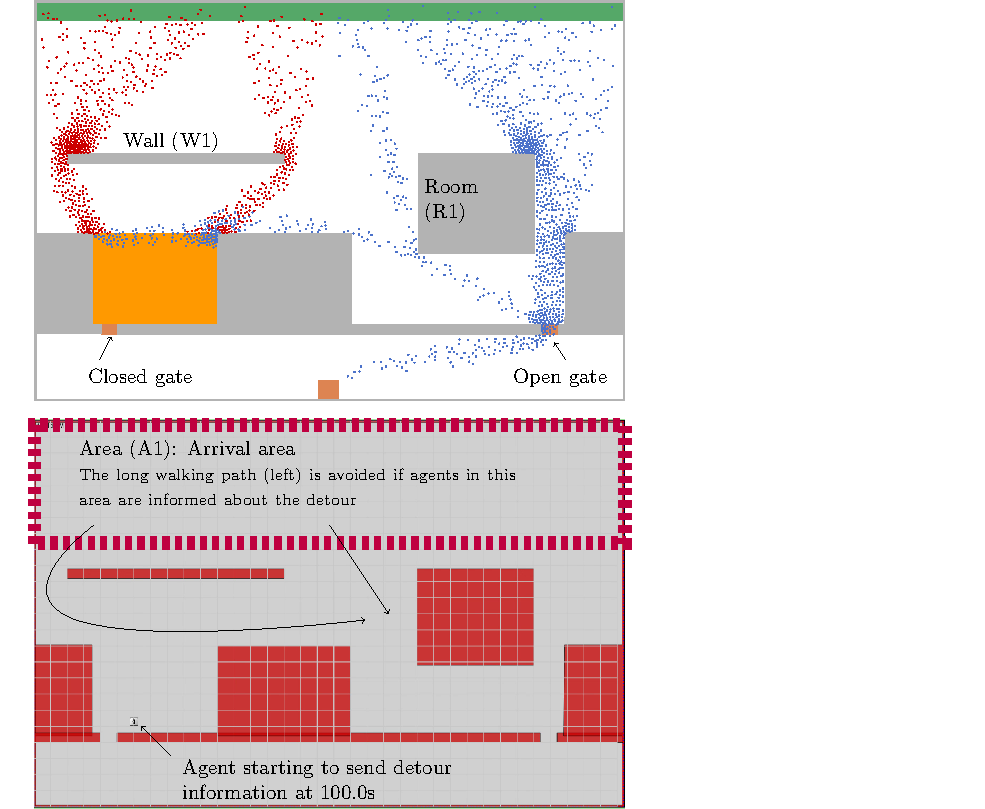
\includegraphics[width=11cm,clip,trim={0.5cm 0 6.0cm 0}]{../figures/investigation/Informationsverbreitung/scenario.pdf} 
\caption[Worst case scenario for investigating information dissemination in a mobile crowd]{Worst case scenario for investigating information dissemination in a mobile crowd.  Representation of the scenario in \textit{Vadere} (top) and \textit{OMNeT++} (bottom). The size of the scenario is $176\,\text{m}\, \times \,129\,\text{m}$. The grid with $5\,\text{m}$ cell width provides orientation (bottom). The agents (blue and red circles) walk from the green source (top) to the target (bottom) on different routes. Agents marked red take a detour, since the left gate (brown area) is closed. The orange area is the area where the closure is in their line-of-sight, so that they start to detour. }
\label{fig:InfoDissSzenario}
\end{figure}




To evaluate the reliability of information dissemination, I propose the following criterion:
\begin{itemize}
\item The information dissemination is reliable if the \textit{dissemination time} $t_{diss}$ does not exceed the threshold value $t_{threshold}$: $t_{diss}\leq t_{threshold}$. Otherwise, if $t_{diss} > t_{threshold}$, information propagation is not reliable.
\end{itemize}
As threshold value I choose $t_{threshold}=10$\,s because within $10$\,s even running pedestrians ($3.0\,\text{m/s}$) receive the information within the arrival area (176\,m$\times$30\,m) where a change of the route choice would not increase the length of the walking path.

To check the plausibility of the simulation results, I compare the \textit{dissemination time} with the statistics of the microscopic quantity of interest \textit{packet lifetime}. The \textit{packet lifetime} describes how long the transmission of a packet takes. 
I expect that the maximum value of the \textit{packet lifetime} and the \textit{dissemination time} have the same order of magnitude. I do not expect that they are equal, since information is transmitted over intermediate nodes. If so, multiple packets are necessary, and, the time it takes to receive information becomes the sum of all \textit{packet lifetimes}. 





\subsection{Model and implementation of the crowd guidance system}

The simulation model of the crowd guidance system is composed of several component models, see Tab.~\ref{tab:composedmodelstudy1}. In the following, the component models are briefly introduced. It is explained why a certain model is chosen for the investigation and hot it is implemented in the \textit{CrowNet} simulator.

\begin{table}[hbt!]
\begin{footnotesize}
\begin{tabular}{|p{2cm}|p{2.6cm}p{3.2cm}p{5cm}|}
\hline
\textbf{Component} & \textbf{Sub-component} & \textbf{Model}  & \textbf{Implementation (Simulator)} \\ \hline
Crowd  & Locomotion model & Optimal Steps Model & OptimalStepsModel (Vadere) \\ \cline{2-4}
& Perception model &  Assumption: info is always perceived & impl. in UdpDetourApp (CrowNet)  \\ \cline{2-4}
& Cognition model & Assumption: 100\% compliance & UdpDetourApp (CrowNet/app.)  \\ \hline

Controller &
Time stepping alg. & Fixed interval (default: 1s) & UdpDetourApp (CrowNet/app.)  \\ \cline{2-4}
&  Route recommendation alg. & None (static information: Gate closed) & Not needed \\ \hline

Network & Application layer & Detour application &  UdpDetourApp  (CrowNet/app.) \\ \cline{3-4}
&& Receive and forward information &  UdpDetourAppVadere  (CrowNet/app.) \\ \cline{2-4}
&Transport layer & Udp  & {Udp} (inet) \\ \cline{2-4}
&Network layer & Ipv4  &{Ipv4NetworkConfigurator} (inet) \\ \cline{2-4}
&Data Link layer & acc. IEEE 802.11 & {Ieee80211MgmtAdhoc} (inet)   \\ \cline{2-4}
&Physical layer &  & \\  
&$\rightarrow$ Channel model & acc. IEEE 802.11 & {Ieee80211DimensionalRadio} and Ieee80211DimensionalRadioMedium (inet) \\ 
&$\rightarrow$ Obstacle Model & Ideal Obstacle model & IdealObstacleLoss (inet)  \\ 

\hline
\end{tabular} 
\end{footnotesize}
\caption[Component models for investigating information dissemination in a crowd]{Component  models for investigating information dissemination in a crowd. If not specified, I use parameter values and settings for the component models. The mobile network model is composed of the protocol stack and the channel model. Importantly, the ideal obstacle model is used to model transmission failures due to shadowing: The transmission fails if agents are not in line-of-sight.}
\label{tab:composedmodelstudy1}
\end{table}




\subsubsection{Crowd behavior}
I assume that all people follow the recommendation to take the alternative route immediately. This assumption may be optimistic, but it should not affect the macroscopic quantities of interest: Even if only a part of the crowd followed the route recommendation, the left stream in Fig.~\ref{fig:InfoDissSzenario} would become wider because non-compliant agents continue to walk downwards while compliant agents turn right.
Nevertheless, the agents form a connected graph within the arrival area. As a consequence, the topology of the network would be similar.  The transmission of individual packets might change, but this should not affect the macroscopic \textit{dissemination time}.
 

After receiving detour information, the target of agent is directly changed without modeling the perception or cognition. The targets are set in the \lstinline{UdpDetourApp} (\textit{OMNeT++}) when an agent receives the information over the mobile network, see Tab.~\ref{tab:composedmodelstudy1}. The \lstinline{UdpDetourApp} then triggers the target change in \textit{Vadere} via the Traffic Control Interface (TraCI). 
To model the locomotion behavior, the Optimal Steps Model is used that is implemented in the  \textit{Vadere} simulator.



\subsubsection{Route recommendation generation}
In the scenario, there is no need for a sophisticated route recommendation algorithm because there is only one route left: This route is recommended all the time. Thus, there is no need to integrate the \textit{flowcontrol} simulator. Instead, a simple redirection model is implemented in the \lstinline{UdpDetourApp} application of the \textit{OMNeT++} module, see Fig.~\ref{fig:study1Simulatorsinvolved}. The redirection model sends static information (`The left gate is closed. Please use the right gate').


\begin{figure}[hbt!]
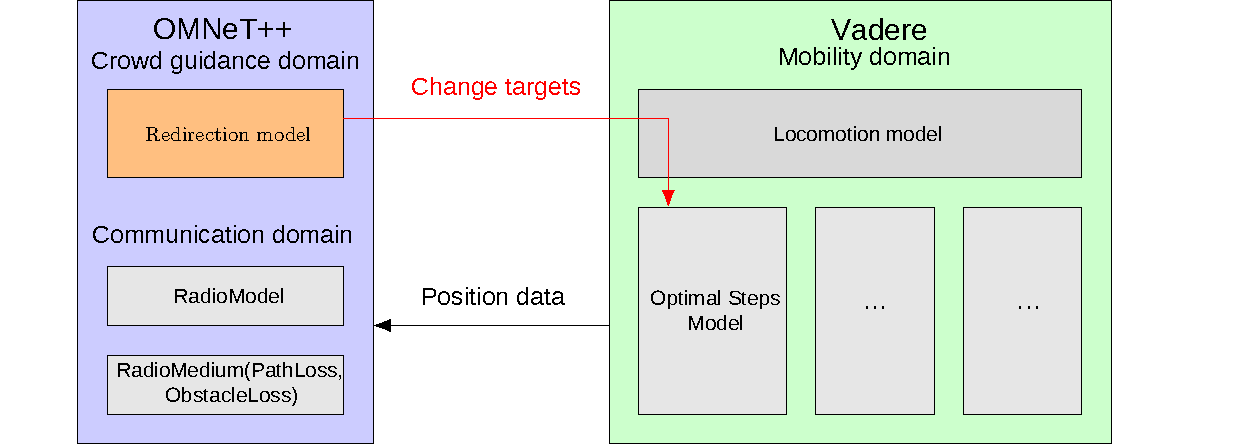
\includegraphics[width=\textwidth,trim={0.2cm 0 1cm 0cm}]{figures/investigation/Informationsverbreitung/ModelInteraction.pdf}  
\caption[Simulation approach in the information dissemination study]{Simulation approach in the information dissemination study. The simulators \textit{OMNeT++} and \textit{Vadere} communicate over the Traffic Control Interface. When detour information has been received in the mobile networks simulation (left), the targets are changed in the crowd simulation (right). Agents' positions from the crowd simulation are shared at the simulation time step of the \textit{Vadere} simulator (0.4s). Image as in my publication~\cite{mayr-2021-com}. }
\label{fig:study1Simulatorsinvolved}
\end{figure}




\subsubsection{Information dissemination through direct communication}

In my investigations I want to test the worst case. Therefore, I suggest to use direct communication according to the IEEE 802.11p standard. If one can inform a mobile crowd based on this technology, it is likely that more advanced technologies based on IEEE 802.11bd or cellular communication may also be suitable. 
Therefore, models for the 802.11p standard are selected on the link and physical layer. The link layer model   handles the sending and reception process of data frames that are passed from device to device. There are no control or management frames. As implementation the module \textit{Ieee80211MgmtAdhoc} from the \textit{INET} framework is used.

The signal modeling is specified at the physical layer. 
To model the signal power in the analog domain, a models are used that describes the change of the signal power over time and frequency: 
 the \textit{Ieee80211DimensionalRadio} model in conjunction with the \textit{Ieee80211DimensionalRadioMedium} model from the \textit{INET} library.

To capture the signal attenuation caused by obstacles, I choose the Ideal Obstacle Model to model the worst case:  If there is an obstacle in line-of-sight, there is no signal strength at all. In a real-life use case, the signal would be attenuated. Therefore, I believe that information dissemination is successful in real life, when it is successful in the simulation because conditions are milder. Using the Ideal Obstacle Model has another advantage: No permeability of the obstacles needs to be defined which keeps the dimensionality of the parameter space low. As implementation the \textit{IdealObstacleModel} from \textit{INET} is used.
 

The sending of the route recommendation is modeled as a mobile application on the application layer. When the application is started, it sends the redirection recommendation at fixed time intervals. Packets are broadcasted via a link local broadcast. No routing protocol is used. The application is implemented as a finite-state machine in the \textit{OMNeT++} module of the \textit{CrowNet} simulator, see Fig.~\ref{sec:controllermodel}. Note that in the scenario only one agent next to the closed gate sends route recommendations. Other agents only receive and forward the information.

Every agent has an application assigned that receives and forwards detour information. The application manages the change of the targets over the Traffic Control Interface. As soon as the detour information is received, the destination contained in the route recommendation is set for the agent. Then, the packet is forwarded via broadcast. An internal timer ensures that the route recommendation is only processed once. This helps to avoid a broadcast storm. As implementation, the \textit{UdpDetourAppVadere} application is implemented in the \textit{OMNeT++} module.



\begin{figure}[hbt!]
\centering
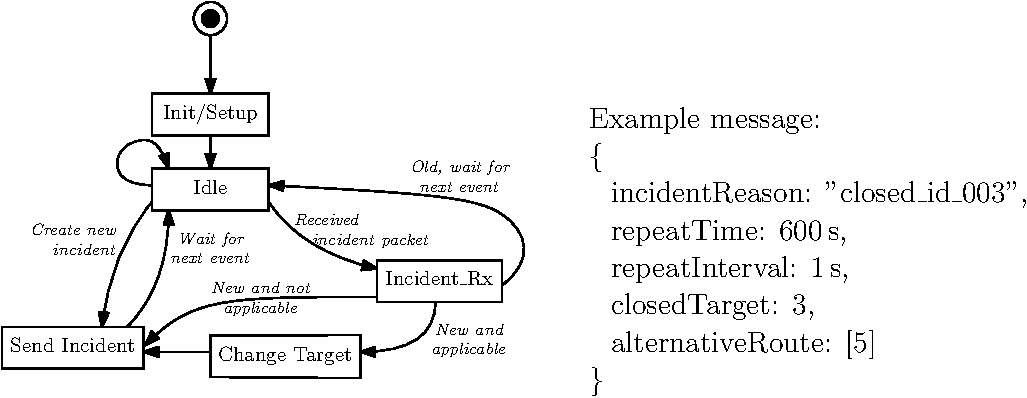
\includegraphics[width=0.9\textwidth]{figures/investigation/Informationsverbreitung/ControlModel.pdf} 
\caption[Controller model generating and forwarding detour information]{Controller model generating and forwarding detour information. Since the left gate (target id=3) is closed, agents are redirected to the right gate (target id=5). The information is provided in time intervals of $1\,s$. 
Image as in my publication~\cite{mayr-2021-com}.}
\label{sec:controllermodel}
\end{figure}





\subsection{Minimal crowd size to avoid shadowing}

In the first sub-study, I want to find out the minimum number of crowd members necessary in my scenario to ensure that the dissemination of route recommendation does not fail due to shadowing. I use the minimum number in the next sub-study as lower bound for an uncertain parameter when conducting an uncertainty quantification study.


\subsubsection{Methodology: varying the crowd size}
To find out how many crowd members are needed to avoid shadowing, the parameter \textit{number of agents} is varied between 20 and 150.  I choose a lower bound of 20 agents due to the following consideration. To prevent shadowing, at least 8 nodes (2$\times$4) are needed: four agents around the wall (W1) and four agents around the room (R1), see Fig.~\ref{fig:InfoDissSzenario}. Another node is required to transport the information to the target area. Since agents' positions are continuously changing, I choose 20 nodes to be on the safe side. I choose an upper bound of 150 agents because one can assume that agents form a connected chain which prevents the effect of shadowing. In total, 500 samples are generated which requires to run the simulation 500 times. 

Since the number of agents is still low, it is likely that the information distribution fails due to shadowing rather than interference. Therefore, I assume, that shadowing is present when the information dissemination fails, that is, when less than $95\,$\% of the agents are informed after $10\,\text{s}$: $p=0.95, t_{threshold}=10\,\text{s}$.  
%I choose discrete parameter values: 20.00, 20.26, 20.52, ... , 149.74, 150.00. Please note that there are of course no half or quarter agents: the number of agents is will be rounded. The decimal place only changes random objects in the simulation. This allows me to take into account the stochastic behavior of pedestrian flows without having to generate different seeds.
%Die ist aus meiner Sicht in dieser Untersuchung notwendig, da die Abschattung zufällig durch die Agentenpositionen entsteht. Die Positionen hängen dabei wiederum von den Laufgeschwindigkeiten der Agenten ab. Da diese aus einer Zufallsverteilung gezogen werden, gehe ich davon aus, dass 

%Bei einer Änderung des seeds laufen die Personen mit anderen Laufgeschwindigkeiten, wodurch sie neue Positionen einnehmen, was Abschattung auflösen oder begünstigen kann. 


\subsubsection{The information dissemination fails due to shadowing}
To ensure that shadowing causes the dissemination failure I randomly select samples with $t_{dissemination}>10\,\text{s}$. I observe that the crowd is indeed temporarily separated by obstacles during the information dissemination process (simulation time $\in [100\,\text{s}, 110\,\text{s}]$), see Fig.~\ref{fig:shadowingexample}. One can observe three separated crowds: A crowd on the left, a crowd on the right and a crowd at the bottom, each represented by blue connecting lines between them. The left crowd is in line-of-sight with the crowd on the right which allows them to pass on information. However, the crowd at the bottom is still shadowed by a wall, so that the four agents close to the target are not informed within $10\,\text{s}$. As a result, the information degree is only  81\,\% after 10\,s (17 of 21 agents have been informed). The visual check strongly indicates that the information dissemination indeed fails due to shadowing when the parameter \textit{number of agents} has a low value.  

\begin{figure}[hbt!]

\begin{tikzpicture}
\node[] at (0,0) {\includegraphics[height=5cm]{./investigation/Informationsverbreitung/Sample_0_shadowing_study/shadowing_sample_0_0.pdf} 
};
\node[] at (8,0.6) {\includegraphics[height=5cm,trim={1.1cm 0.8cm 0cm 0cm},clip]{./investigation/Informationsverbreitung/Sample_0_shadowing_study/InformationDegree.pdf}
};
\node[font=\small, fill=white, text width=7.5cm,align=center] at (7.8,-2.5)  {Time in s  \\ (after info. dissemination started)};
\node[font=\small, fill=white, text width=5.5cm,rotate=90, align=center] at (4.25,0.0)  {Proportion of informed agents in \%};
\draw[color=orange,dashed] (-3.65,0.8) rectangle (3.65,2.45);
\node[font=\tiny,color=orange] at (-2.1,1.9)  {Redirection area (dashed)};
\node[font=\tiny, text width=2cm] at (-1.4,-1.6)  {Information source};
\end{tikzpicture}
\caption[Partially informed crowd due to shadowing]{Partially informed crowd due to shadowing. The crowd is separated by obstacles (see red lines through obstacles on the left). As a consequence, only 17 out of 21 (81\,\%) agents in total are informed after 10\,s (right). Agents in the arrival area have been informed successfully after 3.2\,s (intersection of the orange line and the red threshold line on the right) because agents form a chain in this area (see blue lines connected to the information source on the left). }
\label{fig:shadowingexample}
\end{figure}
 




\subsubsection{Probability for shadowing in dependency of the crowd size}

To determine the probability for shadowing in the scenario, the values of the parameter \textit{number of agents} are grouped into bins. For each bin, it is counted how often shadowing was present. To obtain the probability the count is normalized by the total number of samples. The result is depicted in Fig.~\ref{fig:shadowing}. 

\begin{figure}[hbt!]
\includegraphics[width=\textwidth]{../figures/investigation/crownetOutput/shadowing/ProbabilityforShadowingCrowdSize.pdf} 
\caption[Information dissemination time and probability for shadowing]{Information dissemination time and probability for shadowing. The information dissemination is successful when the dissemination time is $\leq10\,\text{s}$ (left).  Note that the information dissemination time is a multiple of the time step size $0.4\,\text{s}$. The more agents, the less likely shadowing is (right). In the research scenario, shadowing is no longer present when the crowd has more than 110 members. }
\label{fig:shadowing}
\end{figure}


As expected, the probability of shadowing decreases over the uncertain parameter \textit{number of agents}. In the scenario, there appears to be no more shadowing with more than 110 agents. Below this threshold, shadowing is likely to occur. However, one cannot predict whether shadowing occurs for a specific sample, since the crowd locomotion is stochastic: Agents' walking speeds are randomly drawn from a normal distribution. A change of the seed or a slightly different value of a parameter changes agents positions. One can observe that communication can even succeed if the \textit{number of agents} is small: For 30 agents only, the \textit{dissemination time} is less than $5.2\,\text{s}$, see Fig.~\ref{fig:shadowing} (left). However, this is a stochastic effect that cannot be controlled.



\subsubsection{Summary of the shadowing study: shadowing is prevented with a sufficient dense crowd}
The first sub-study suggests that with enough well distributed agents present, loss of information through shadowing can be completely avoided. In the scenario 110 agents sufficed to spread detour information in a crowd in less than 10 seconds. I conclude this is enough time to inform agents about a closure before they take a closed route.



\subsection{Effect of uncertainties on the information dissemination}

\subsubsection{Motivation for quantifying uncertainties}
%We know from the previous study that information distribution using direct communication can fail when crowd sizes are small. In this sub-study, I will assess how reliably information is disseminated in the absence of shadowing. 


The crowd size in real-life scenarios, like at a train station or a festival, is often uncertain. Apart from the crowd size, there are additional unknowns, such as the transmitter power of smartphones. I aim to understand how such uncertainties impact the reliability of the information dissemination. 
Therefore, uncertainty quantification methods are applied. I choose a surrogate-based approach with polynomial chaos expansions to reduce the computational effort because a single simulation run can take several hours.

Forward propagation is employed to assess the effect of uncertain parameters on the quantities of interest. A global sensitivity study is conducted to quantify the influence of parameters.

The sub-study is structured as follows. First, the set of parameters and quantities of interest is introduced. Second, the simulation pipeline is described which comprises the construction of the polynomial chaos expansions. Finally, the results are discussed. I expect the reader to be familiar with the theory on polynomial chaos expansions, forward propagation and global sensitivity analysis (see Section~\ref{sec:uq}).


\subsubsection{Parameter selection for the uncertainty quantification}
I consider two uncertain parameters that I think are particularly interesting for a crowd guidance system: the \textit{number of agents} and the \textit{transmission interval}, see Tab.~\ref{tab:parameterstudy1}. The parameter \textit{transmitter power} only serves as a control. 

\begin{table}[hbt!]
\centering
\begin{tabular}{@{}llrrl@{}}%
\toprule
Parameter                        & Unit & Distribution & Sample points                                  \\ \midrule
Number of agents $n$ & 1    & U(200,2500) & 415, 1325, 2235    \\
Transmitter power $p$      & mW   & U(2.0, 20.0) & 4.03,11.00, 17.97     \\
Transmission interval $si$        & s   & U(0.8,2.8)   & 1.0, 1.8, 2.6       \\
\bottomrule
\end{tabular}%
\\ \vspace{0.3cm}
\caption[Uncertain parameters in the information dissemination study]{Uncertain parameters in the information dissemination study. The three parameters are used in the forward propagation and in the global sensitivity analysis. Since the shape of the distributions are unknown, I use uniform distributions.   Three sample points for each parameter are needed to construct a polynomial chaos expansion of order\,$=2$. In total, there are $27\,(=3^3)$ samples.   }%
\label{tab:parameterstudy1}%
\end{table}%

The first parameter is the \textit{number of agents}. The previous part of the study demonstrated how communication fails due to shadowing when the \textit{number of agents} is low. A high \textit{number of agents} can, in turn, lead to interference in the mobile network or congestion in passenger traffic. Thus, this parameter controls the dynamics of  the complex socio-technical system composed of the crowd and the mobile network. Since I do not know the distribution type of the parameter, I use a unit distribution. As lower bound I use a \textit{number of agents} of 200 (the previous study required at least  110 to prevent shadowing). As upper limit I choose 2500.  More agents would lead to a congestion where agents do no longer move at all. I want to avoid a change of the crowd dynamics because this opens the question whether changes in the information dissemination process are caused by a change of the crowd dynamics or by a change of the mobile network.  

The second parameter is the \textit{transmission interval}. At the simulation time 100\,s, one agent next to the closed gate (see Fig.~\ref{fig:InfoDissSzenario}) starts to send detour information repeatedly over broadcast.   The \textit{transmission interval} is the time in between two broadcast rounds. The repetitions increase the probability that information is successfully disseminated even if the communication locally or temporarily breaks due to interference. However, the smaller the transmission interval, the higher the risk for collisions and interference. Therefore, I choose a lower bound of 0.8\,s. As upper bound I choose 2.8\,s which means that the broadcast is re-started four times within 10\,s: 0\,s, 2.8\,s, 5.6\,s, 7.8\,s. I argue four chances should be enough to disseminate information. 


The third parameter is the \textit{transmitter power} of the smart phone's antennas. In combination with  other parameters such as the receiver sensitivity of the antennas, this parameter determines the range for communication. It serves as a control because this parameter does not have an effect: The scenario is sufficiently small so that agents are always in communication range (see Appendix~\ref{sec:networkparameters}). I choose a parameter range [2.0\,mW, 20.0\,mW] which is typical for many types of smartphones.  % I assume default values for all other parameters that influence the range.

\subsubsection{Selection of quantities of interest}

I am interested in six scalar quantities of interest:
\begin{itemize}
\item \textit{TimeAll}: Dissemination time ($p=0.95$) referring to all agents: How long does it take until 95\,\% of the agents are informed about the detour? Accuracy: time step size 0.4\,s. \textit{SI-Unit: s}
\item \textit{TimeArrArea}: Dissemination time ($p=0.95$) referring to agents in the arrival area: How long does it take until 95\% of the agents are informed in the arrival area? Accuracy: time step size 0.4\,s. \textit{SI-Unit: s}
\item \textit{NumAgents}: I use the number of agents as control (similar to the control parameter transmitter power; here the number of agents is a measurement quantity not a parameter). \textit{SI-Unit: 1}
\end{itemize}
Please note that the \textit{dissemination times} are always a multiple of the simulation step size of the \textit{Vader}e simulator (0.4\,s). 

The information is successfully disseminated when at least $p=95$\% of the agents have been informed. A proportion of $p=95$\% ensures that the information degree is not underestimated due to short-term fluctuations caused by informed agents that reach the target or leave the reference area.

To check the plausibility of the simulation results, I compare the \textit{dissemination time} with the statistics of the microscopic quantity of interest \textit{packet lifetime}. The  \textit{packet lifetime} describes how long it takes that a packet is transmitted in the mobile network from a sender to a receiver.  %If the route recommendation fits into a packet and if the transmission takes place without intermediate nodes, 

\begin{itemize}
\item \textit{MaxPackLifetime}: maximal packet lifetime. \textit{SI-Unit: s}
\item \textit{MedPackLifetime}: median packet lifetime. \textit{SI-Unit: s}
\item \textit{MinPackLifetime}: minimal packet lifetime. \textit{SI-Unit: s}
\end{itemize}

I expect that the \textit{maximal packet lifetime} and the \textit{dissemination times} have the same magnitude. I further expect that the \textit{maximal packet lifetime} is higher than the information dissemination time since the \textit{dissemination time} refers to the 95\,\% of the agents who get informed first. I check both expectations when analyzing the results.



\subsubsection{Methodology: forward propagation and sensitivity analysis using polynomial chaos expansions}
I use polynomial chaos expansions for forward propagation and global sensitivity analysis. In total, I construct 6 polynomial chaos expansions: one for each quantity of interest, see Fig.~\ref{fig:uqmethodologystudy1}. The same order is chosen for all polynomial chaos expansions. Therefore, the same sampling can be used for their construction.
For the polynomial degree, I choose a quadratic approach (order\,=\,2) to capture linear and quadratic behaviors of the quantities of interest in dependency of the uncertain parameters. To model plateaus or rapid changes, higher orders would be necessary. However, I cannot further increase the order since the number of samples grows exponentially and running one simulation can take several hours.  To construct a polynomial chaos expansion of order 2, three grid points are required for each parameter. The grid point values can be found in Tab.~\ref{tab:parameterstudy1}. In total, this makes 27 samples or simulation runs. 

\begin{figure}[hbt!]
\includegraphics[width=\textwidth]{./investigation/Informationsverbreitung/uqprocedure.pdf} 
\caption[Parameters and quantities of interest for the forward propagation and sensitivity analysis]{Parameters and quantities of interest for forward propagation and global sensitivity analysis. I use polynomial chaos expansions for forward propagation and  sensitivity analysis. For each of the six quantities of interest, a polynomial chaos expansion of order 2 is constructed. With three parameters, 27 samples must be executed. From the expansions the first and total order sensitivity indices of the parameters and the statistical moments of the quantities of interest are computed. }
\label{fig:uqmethodologystudy1}
\end{figure}


Due to the long simulation duration of up to four hours, I do not carry out any repetitions, although random effects are present in my system. I argue that the influence of random effects is negligible 
because due to the \textit{number of agents} in the system the crowd forms a coherent communication network. I expect that there are local changes in the communication due to stochasticity. For example in one case agent (1) communicates directly with agent~(2) and agent~(3). In another case, agent~(1) communicates with agent~(2)~who passes the information on to agent~(3). As long as the network is coherent, I claim that such local effects have a negligible effect on the macroscopic \textit{dissemination times} or the statistical moments of the \textit{packet lifetime}. In fact, a preliminary study with one sample demonstrated that the quantities of interest do not differ qualitatively for the three tested seeds. This supports my claim, without being a general proof.

The simulation study is carried out with the \textit{SUQ-controller} module of \textit{CrowNet}. To reduce the total simulation time, 8 simulations are run in parallel using the virtual machine that is described in Appendix~\ref{sec:VirtualMachine}.





\subsubsection{Verification of the polynomial chaos expansions and plausibility check}
 
First, the correct construction of the polynomial chaos expansions is verified. The first control hypothesis is that the parameter \textit{transmitter power} has no influence. Tab.~\ref{tab:indicessensit} shows that this is indeed the case. Both the first and the total sensitivity index are zero, indicating that the parameter has no influence. 
The second control hypothesis is that the quantity of interest \textit{number of agents} depends only on the uncertain parameter \textit{number of agents}. This is indeed the case: Tab.~\ref{tab:indicessensit} shows that the first and total index of the parameter \textit{number of agents} is 1.0. All other indices are zero (see line \textit{NumAgents} in Tab.~\ref{tab:indicessensit}), which means that the other parameters have no influence. 
%With this in mind, I consider the construction of my polynomial chaos expansions as verified. I will not examine the control quantities "transmitter power" any further in the following.

Second, the simulation results are checked for plausibility. Tab.~\ref{tab:qoimoments} depicts the statistical moments of the quantities of interest. One can observe that the expected values of the \textit{median packet lifetime} (5.046\,s) and the \textit{dissemination time} (5.0\,s ... 5.4\,s) are equal for an accuracy of 0.4\,s. Importantly, they have the same order of magnitude. Therefore, the simulation results are plausible.

\begin{table}[hbt!]

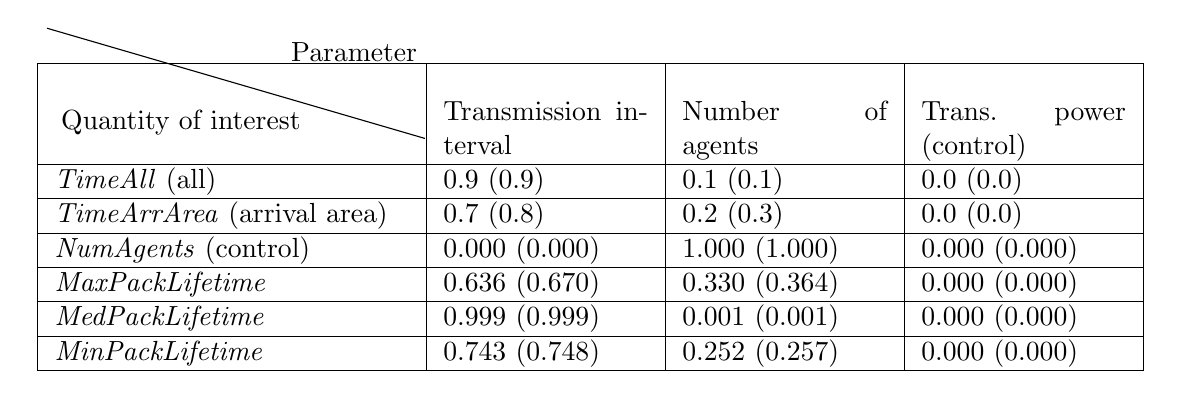
\begin{tikzpicture}

\node[] at (0,0) {
    \begin{tabular}{|p{4.5cm}|p{2.6cm}|p{2.6cm}|p{2.6cm}|}
    \hline
     & && \\
         &Transmission interval & Number of agents & Trans. power (control)  \\ \hline
       \textit{TimeAll} (all) & 0.9 (0.9) & 0.1 (0.1) & 0.0 (0.0) \\ \hline
        \textit{TimeArrArea} (arrival area) & 0.7 (0.8) & 0.2 (0.3) & 0.0 (0.0) \\ \hline
         \textit{NumAgents} (control)  & 0.000 (0.000) & 1.000 (1.000) & 0.000 (0.000) \\ \hline
         \textit{MaxPackLifetime} & 0.636 (0.670) & 0.330 (0.364) & 0.000 (0.000) \\ \hline
        \textit{MedPackLifetime}  & 0.999 (0.999) & 0.001 (0.001) & 0.000 (0.000) \\ \hline
       \textit{MinPackLifetime}  & 0.743 (0.748) & 0.252 (0.257) & 0.000 (0.000) \\ \hline
    
 \end{tabular}
 
 };
 \draw[] (-6.9,2.4) -- (-2.1,1);
  \node[] at (-5.2,1.2) {   Quantity of interest   };
    \node[] at (-3,2.1) {   Parameter    };

\end{tikzpicture}
 
\caption[First and total order sensitivity indices for the quantities of interest]{First and total order sensitivity indices for the quantities of interest. The indices are estimated using polynomial chaos expansions. The total effect indices are in brackets. As expected, the control parameter \textit{transmitter power} does not have any influence (indices: 0.0). The quantity of interest \textit{NumAgents} serves as a control: It only depends on the uncertain parameter \textit{number of agents}.  }
\label{tab:indicessensit}
\end{table}




%For the redirection of pedestrians, the information dissemination time in the redirection area is important. I expect that most of the people will decide on a route in this area and then stick to the route which makes them take a detour when they have not been informed successfully. This is why I look at the dissemination time referring to the redirection area. Tab.~\ref{tab:qoimoments}, one can expect that it takes about 3.2s ... 3.6s to inform the crowd in the redirection area. This might be slow at a scale of mobile networks communication, but it is fast at a scale of crowd locomotion: even fast pedestrians (2.2m/s) walk 8m far in 3.6s. I would expect that they have not already entered a route in many real life scenarios such as a train station. Depending on the parameters number of agents and sending interval, it can also take longer: the standard deviation is not zero (0.8s). However, as we have seen, this mostly depends on the choice of the sending interval which we are in control of. 

\begin{table}[hbt!]
\centering
\begin{footnotesize}


    \centering
    \begin{tabular}{p{3.3cm}p{2.5cm}p{2.3cm}p{2.8cm}}
    \hline
        Quantity of interest & ~ & Expected value & Standard deviation \\ \hline
       Dissemination time in s & \textit{TimeAll} & [5.0 ... 5.4[ & 1.2 %... 1.2 (=$\sqrt{1.2^2 + (0.4/2)^2}$) %/ 
       \\
        ~ & \textit{TimeArrArea} & [3.2 ... 3.6[ & 0.8 % ... 0.8 (=$\sqrt{0.8^2 + (0.4/2)^2}$)  
        \\ 
         Packet lifetime in s & \textit{MaxPackLifetime} & 7.548 & 0.730 \\ 
        ~ & \textit{MedPackLifetime} & 5.046 & 0.545 \\ 
        ~ & \textit{MinPackLifetime} & 4.973 & 0.701   \\ \hline
    \end{tabular}
    \end{footnotesize}
    \caption[Statistical moments for the quantities of interest]{Statistical moments for the quantities of interest. The statistical moments are estimates, derived from polynomial chaos expansions. 
    As the \textit{information degree} is only measured every 0.4\,s in \textit{Vadere}, the \textit{dissemination time} can only be specified with an accuracy of 0.4\,s. Accordingly, I use 1 decimal place only and provide  ranges for the expected values and standard deviations for the \textit{dissemination times}. Note that the range limits of the standard deviations differ in the second digit only under the assumption that the error of the standard deviation is 0.4\,s. }
\label{tab:qoimoments}
\end{table}




\subsubsection{Influence of the parameters \textit{number of agents} and \textit{transmission interval}}
Next the influence of the two parameters \textit{number of agents} and \textit{transmission interval} is analyzed. Tab~\ref{tab:indicessensit} shows their sensitivity indices for each quantity of interest. One observes that the first and the total sensitivity index (shown in brackets) are similar. This indicates that there are negligible interaction effects (second order effects) between the parameters. Thus, I use the first sensitivity index from now on.


The parameter \textit{number of agents} has only little influence on the information dissemination: For the \textit{median packet lifetime}, the sensitivity index is almost zero. This indicates no effect at all. For the \textit{minimum} and \textit{maximum packet lifetime}, the indices are low with 0.252 and 0.330 respectively. In fact the true values might be even lower because the indices also encounter variance caused by the varying sample size. The more agents, the more packet transmissions, and the more, accurately the bounds of the \textit{packet lifetime} distribution are captured. For the evaluation of the dissemination process, I, therefore, look at \textit{dissemination times} that are independent of the sample size.

The dissemination of information referring to all agents seems only slightly influenced (\textit{TimeAll} index: 0.1) by the \textit{number of agents}, see Tab.~\ref{tab:indicessensit}.
For agents in the arrival area, the influence is higher but still low (\textit{TimeArrArea} index: 0.2). The low influence can be verified visually in Fig.~\ref{fig:infodissplotdep}. For each \textit{transmission interval}, the \textit{dissemination time} is plotted over the \textit{number of agents}. The  data points correspond to the samples used for the polynomial chaos expansion. One can observe that the \textit{dissemination time} hardly changes over the \textit{number of agents} (left). For the arrival area (right), the \textit{dissemination time} changes over the \textit{number of agents} for certain \textit{transmission intervals}. I attribute this to the fact that fewer agents are in the arrival area than in the entire topography. Therefore, the local transmission of packets has a stronger influence on the \textit{dissemination time}. 
\begin{figure}[hbt!]
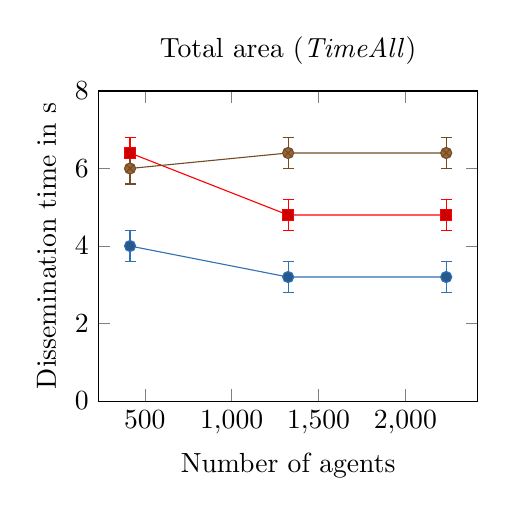
\begin{tikzpicture}
\begin{axis}[xlabel=Number of agents,ylabel=Dissemination time in s,title=Total area (\textit{TimeAll}), ymax=8,ymin=0,width=6.4cm]
\addplot+ [error bars/.cd,y dir=both,y fixed=0.4,
] table [x=Number,y=All,meta=Time] {
Time Number	All	Area
1.0	415	4.0	3.2
1.0	1325 3.2 3.2
1.0	2235 3.2 2.0
};
\addplot+ [error bars/.cd,y dir=both,y fixed=0.4,
] table [x=Number,y=All,meta=Time] {
Time Number	All	Area
1.8	415	6.4	2.8
1.8	1325 4.8 2.8
1.8	2235 4.8 2.8
};

\addplot+ [error bars/.cd,y dir=both,y fixed=0.4,
] table [x=Number,y=All,meta=Time] {
Time Number	All	Area
2.6	415	6.0	6.0
2.6	1325 6.4 3.6
2.6	2235 6.4 3.6
};
\end{axis}
\end{tikzpicture}
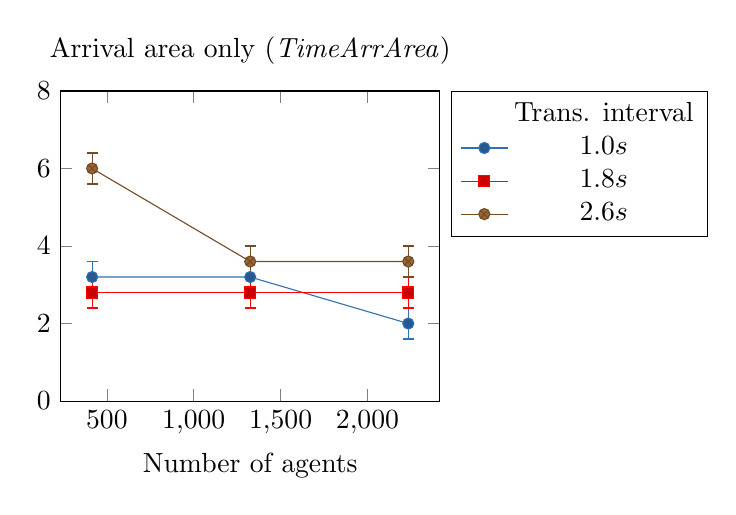
\begin{tikzpicture}
\begin{axis}[xlabel=Number of agents,legend entries={Trans. interval,$1.0s$,$1.8s$,$2.6s$},title=Arrival area only (\textit{TimeArrArea}),ymax=8,ymin=0,width=6.4cm,legend pos=outer north east]
\addlegendimage{empty legend}
\addplot+ [error bars/.cd,y dir=both,y fixed=0.4,
] table [x=Number,y=Area,meta=Time] {
Time Number	All	Area
1.0	415	4.0	3.2
1.0	1325 3.2 3.2
1.0	2235 3.2 2.0
};
\addplot+ [error bars/.cd,y dir=both,y fixed=0.4,
] table [x=Number,y=Area,meta=Time] {
Time Number	All	Area
1.8	415	6.4	2.8
1.8	1325 4.8 2.8
1.8	2235 4.8 2.8
};

\addplot+ [error bars/.cd,y dir=both,y fixed=0.4,
] table [x=Number,y=Area,meta=Time] {
Time Number	All	Area
2.6	415	6.0	6.0
2.6	1325 6.4 3.6
2.6	2235 6.4 3.6
};
\end{axis}
\end{tikzpicture}
\caption[Dissemination time over number of agents]{\textit{Dissemination time} over number of agents. Due to the time step size, the dissemination time has an accuracy of 0.4\,s indicated by the error bars. The data points correspond to the sample points used to construct the polynomial chaos expansions. The dissemination times hardly change over the \textit{number of agents}. The parameter \textit{transmission interval} has indeed an effect (left). }
\label{fig:infodissplotdep}
\end{figure}



The parameter \textit{transmission interval} has a great influence on all quantities of interest. The index is between 0.636 and 0.999 except for the control, see the column `Transmission interval' in Tab~\ref{tab:indicessensit}. An explanation is that the smaller the \textit{transmission interval}, the more often information is provided and the faster the crowd is informed. 
The influence of the \textit{transmission interval} can be also observed in Fig.~\ref{fig:infodissplotdep}. The larger the \textit{transmission interval}, the larger the \textit{information dissemination}. The  parameter influence is more dominant for the entire population than for pedestrians within the arrival area: The corresponding indices are 0.9 (\textit{TimeAll}) and 0.7 (\textit{TimeArrArea}), see again Tab.~\ref{tab:indicessensit}.


To quantify the uncertainty of the \textit{dissemination times}, I look at their statistical moments, see again Tab.~\ref{tab:qoimoments}. One can expect that the total crowd is informed within  5.0\,s ... 5.4\,s, while the population in the arrival area is informed in 3.2\,s ... 3.6\,s. The standard deviations are 1.2\,s and 0.8\,s respectively. Most importantly, none of the \textit{dissemination times} is larger than 7\,s even if the \textit{number of agents} exceeds 2000, see again Fig~\ref{fig:infodissplotdep}.

\subsubsection{Need of repetitive information provision}

With an increasing number of pedestrians, the probabilities of interference and packet loss increase, see Fig.~\ref{fig:interferencepacketloss}. However, interference seems to affect the information dissemination process only locally.  Fig.~\ref{fig:snapshots} shows one sample where some agents have not been informed after 3.6\,s. These agents are all located on the left-hand side near a dense crowd where the risk of interference is high. 
Despite inferences, agents are still informed within 6.4\,s, see Fig.~\ref{fig:snapshots}. I attribute this to the fact that information is provided repeatedly. If the information dissemination fails locally, the information is received in the next broadcast round. Since agents informed in the first round do not forward information, the risk of interference is reduced for the next rounds. This also explains the high influence of the parameter \textit{transmission interval}.




\begin{figure}[hbt!]
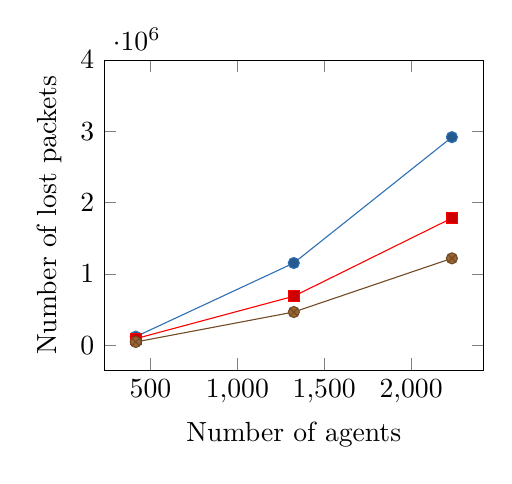
\begin{tikzpicture}
\begin{axis}[xlabel=Number of agents,ylabel=Number of lost packets,width=6.4cm,ymax=4000000]
\addplot+ [] table [x=Agents,y=IncorrectlyReceived] {
id Agents IncorrectlyReceived power
1 415 120407 11
10 1325 1153711 11
19 2235 2918619 11
};
\addplot+ [] table [x=Agents,y=IncorrectlyReceived] {
id Agents IncorrectlyReceived
4 415 92541
13 1325 687913
22 2235 1783373
};
\addplot+ [] table [x=Agents,y=IncorrectlyReceived] {
id Agents IncorrectlyReceived
7 415 46342
16 1325 466153
25 2235 1219119
};
\end{axis}
\end{tikzpicture}
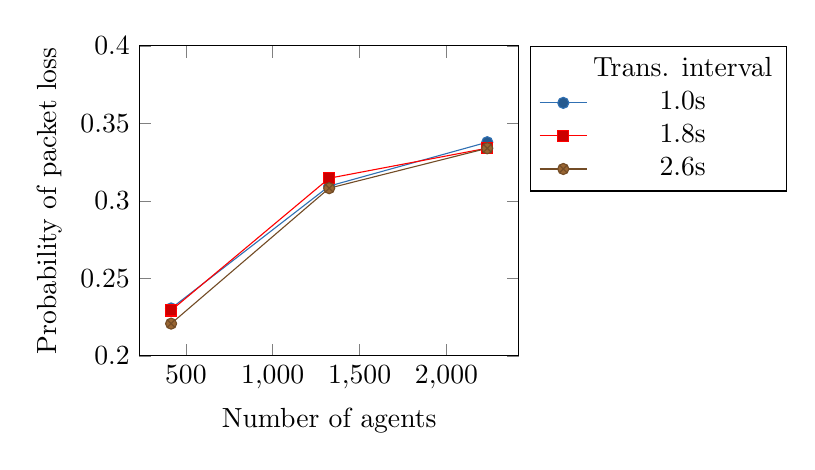
\begin{tikzpicture}
\begin{axis}[xlabel=Number of agents,ylabel=Probability of packet loss,legend entries={Trans. interval,1.0s,1.8s,2.6s},legend pos=outer north east, ymin=0.2, ymax=0.4,width=6.4cm]
\addlegendimage{empty legend}
\addplot+ [] table [x=Agents,y expr=\thisrow{IncorrectlyReceived}/(\thisrow{IncorrectlyReceived}+\thisrow{Passed})] {
id Agents IncorrectlyReceived Passed power
1 415 120407 401675 11 
10 1325 1153711 2573554 11
19 2235 2918619 5720886 11
};
\addplot+ [] table [x=Agents,y expr=\thisrow{IncorrectlyReceived}/(\thisrow{IncorrectlyReceived}+\thisrow{Passed})] {
id Agents IncorrectlyReceived Passed power 
4 415 92541 310980 11 
13 1325 687913 1498629 11
22 2235 1783373 3556361 11
};
\addplot+ [] table [x=Agents,y expr=\thisrow{IncorrectlyReceived}/(\thisrow{IncorrectlyReceived}+\thisrow{Passed})] {
id Agents IncorrectlyReceived Passed power
7 415 46342 163505 11
16 1325 466153 1046453 11
25 2235 1219119 2431961 11
};
\end{axis}
\end{tikzpicture}

\caption[Packet loss caused by interference]{ Packet loss caused by interference. The number of lost packets increases over the \textit{number of agents} (left). The lower the transmission interval, the more often the dissemination process is re-started and the higher the loss is. The probability for interference, estimated by the the number of lost packets divided by the number of total packets, also increases over the \textit{number of agents} (right). The transmission interval has no effect on the probability.  }
\label{fig:interferencepacketloss}
\end{figure}





\begin{figure}[hbt!]
\begin{tikzpicture}
\node[inner sep=0pt] at (0,0){\includegraphics[width=9cm]{./investigation/Informationsverbreitung/Sample_26/info_diss_sample_26_100s_state_part.pdf} };
\node[inner sep=0pt] at (0,-5.5){\includegraphics[width=9cm, trim=0cm 35cm 30.0cm 0cm, clip]{./investigation/Informationsverbreitung/Sample_26/info_diss_sample_26_103_6s_area_informed_part.pdf}};
\node[inner sep=0pt] at (0,-11){\includegraphics[width=9cm]{./investigation/Informationsverbreitung/Sample_26/info_diss_106_4_all_informed_part.pdf}};
\node[text width =7cm] at (8.5,0) {Simulation time: 100.0\,s \\ (Start to disseminate information)};
\node[text width =7cm] at (8.5,-5.5) {Simulation time: 103.6s \\ (95\,\% of agents informed \\ in arrival area)  };
\node[text width =7cm] at (8.5,-11) {Simulation time: 106.4s \\ (95\,\% of agents informed) };

\draw (-3.8,-6.7) circle (0.7);
\node[text width=3.4cm] at (-1.1,-6.5) {Agents not \\ informed yet (red)};

\draw[draw=black, dashed] (-4.5,-5.3) rectangle ++(9,2.0);
\node[text width=8cm] at (0,-3.8) {Arrival area: $>$ 95\,\% of agents informed };


\end{tikzpicture}
\caption[Uncertainty quantification study: Simulation snapshots ]{ Uncertainty quantification study: Simulation snapshots for the design with 2235 agents, a transmitter power of 19.97\,mW and a transmission interval of 2.6\,s. The information dissemination starts at 100\,s. Red agents are unaware about the closure of the gate. After 3.6\,s, the agents in the upper part have been informed. After 106.4\,s 95\,\% of the total population has been informed. }
\label{fig:snapshots}
\end{figure}


\subsubsection{Delays in the information dissemination process}
As expected, the sub-population of agents in the arrival area is informed faster than the total population. Fig.~\ref{fig:infodegree} depicts the information degree for both populations. One can observe that the orange lines (sub-population) cross the 95\,\% threshold earlier than the blue lines (total population). This is plausible, since less agents need to be informed. Interestingly, the information dissemination process shows some delays, see the  plateaus of the graphs in Fig.~\ref{fig:infodegree}. These delays occur because the information is passed via a chain of agents around obstacles. If the communication chain breaks, the transmission is delayed for at least one \textit{transmission interval}. Note that, for the arrival area, the decrease of the information degree in Fig.~\ref{fig:infodegree} (top left) is caused by informed agents leaving the arrival area. 



\begin{sidewaysfigure}
%\thisfloatpagestyle{empty}
\begin{tikzpicture}
\node[inner sep=0pt] at (0,0){\includegraphics[width=7.5cm]{./investigation/crownetOutput/information_diss_time/InformationDegree_Sample_1_0.pdf}};
\node[inner sep=0pt] at (7,0){\includegraphics[width=7.5cm]{./investigation/crownetOutput/information_diss_time/InformationDegree_Sample_4_0.pdf}};
\node[inner sep=0pt] at (14,0){\includegraphics[width=7.5cm]{./investigation/crownetOutput/information_diss_time/InformationDegree_Sample_7_0.pdf}};
\node[inner sep=0pt] at (0,-5.1){\includegraphics[width=7.5cm]{./investigation/crownetOutput/information_diss_time/InformationDegree_Sample_10_0.pdf}};
\node[inner sep=0pt] at (7,-5.1){\includegraphics[width=7.5cm]{./investigation/crownetOutput/information_diss_time/InformationDegree_Sample_13_0.pdf}};
\node[inner sep=0pt] at (14,-5.1){\includegraphics[width=7.5cm]{./investigation/crownetOutput/information_diss_time/InformationDegree_Sample_16_0.pdf}};
\node[inner sep=0pt] at (0,-10.2){\includegraphics[width=7.5cm]{./investigation/crownetOutput/information_diss_time/InformationDegree_Sample_19_0.pdf}};
\node[inner sep=0pt] at (7,-10.2){\includegraphics[width=7.5cm]{./investigation/crownetOutput/information_diss_time/InformationDegree_Sample_22_0.pdf}};
\node[inner sep=0pt] at (14,-10.2){\includegraphics[width=7.5cm]{./investigation/crownetOutput/information_diss_time/InformationDegree_Sample_25_0.pdf}};
\node[text width =7cm] at (11,3.4) {\textbf{Transmission interval}};
\node[text width =7cm] at (3,3) {1.0\,s};
\node[text width =7cm] at (11,3) {1.8\,s};
\node[text width =7cm] at (17,3) {2.6\,s};
\node[text width =7cm] at (-1,0) {415};
\node[text width =7cm] at (-1,-5.1) {1325};
\node[text width =7cm] at (-1,-10.2) {2235};
\node[text width =2cm] at (-4.7,1) {\textbf{Number of agents}};
\end{tikzpicture}
\caption[Information degree over time for a fixed radio transmitter power]{Information degree over time for a fixed radio transmitter power (p\,=\,11\,mW). The information dissemination time is the time that elapses until 95\,\% of the agents are informed in the arrival area (orange curve) or the total area (blue curve). The value p\,=\,95\,\% (red line) ensures that temporal fluctuations, caused by informed agents leaving one of the reference areas, do not have an effect.}
\label{fig:infodegree}
\end{sidewaysfigure} 



\subsubsection{Summary and findings from the uncertainty quantification analysis}
The second sub-study indicates that information can be disseminated in a mobile crowd through direct communication within a few seconds. A global sensitivity analysis showed that the crowd size does not greatly affect the dissemination time, that is, the time it takes to distribute detour information in a crowd. This is fortunate since in a real life application one cannot control the crowd size. The transmission interval, that is the time between two repetitions when detour information is sent, had a big influence on the information dissemination process. The more often information was provided, the faster the entire crowd was informed. 
 
\FloatBarrier

\subsection{Summary, limitations, lessons learned}

\subsubsection{Summary of the two investigations}

In this section I investigated my first research sub-question, that is, how reliably route recommendations are disseminated through direct communication technology in a mobile crowd.
I proposed and applied a two-step procedure to investigate the information dissemination systematically when shadowing is present. First, one examines how shadowing depends on the number of agents in the scenario.  More agents mean a closer distance between nodes in the mobile network. Second, one assesses how quickly information is transmitted when there are sufficiently many crowd members in the system. This procedure allows to separate the effect of shadowing and interference and, thus,  helps to better understand the behavior of the socio-technical system composed of the crowd and the mobile network. To answer my research question, I designed a scenario that reflects worst-case conditions for the direct communication: A person sending the detour information was shadowed by walls and only pedestrians in line-of-sight received detour information through direct communication.
To evaluate the reliability of the information dissemination process, I introduced a criterion that demands that the entire crowd must be informed within a certain time. 
In the first part of the study I varied the number of agents. I found that at least 110 crowd members are necessary to prevent shadowing in the scenario. In the second part, the uncertainty of the information dissemination process was quantified using forward propagation based on polynomial chaos expansions. To quantify the influence of parameters, global sensitivity analysis was applied, again using polynomial chaos expansions. I found that route recommendations were disseminated in a crowd within a few seconds. The number of crowd members had a low effect on the information dissemination when the crowd was dense enough. The transmission interval, that is the time in between two information broadcasts, had a large effect on the information dissemination. The more often information was provided, the faster the entire crowd was informed. In my scenario the fastest information dissemination was achieved with a transmission interval of one second. 


In both studies I assumed that the communication breaks whenever the line-of-sight is broken. In reality, the information provision might be even better thanks to the permeability of materials and to reflections. In short the answer to the first research sub-question is:

\begin{tcolorbox}[title=How reliably are route recommendations disseminated using direct communication in a crowd? (RQ-1)]
Using direct communication technology, route recommendations can be reliably disseminated in a mobile crowd  within a few seconds, provided there are enough crowd members to counteract shadowing.
\end{tcolorbox}



\subsubsection{Limitations}
I would like to point out some limitations of the study, some of them which I will address in my following investigations.


I assumed that all pedestrian immediately and always follow the route recommendation. In reality, pedestrians might not be aware of the mobile message or for some reason my not follow instructions. Therefore, I will assess the effect of compliance in Section~\ref{sec:umleitalgorithmen}.

The topography of the scenario was sufficiently small. Therefore, pedestrian were always in communication range. If the topography was larger, information dissemination may fail.

In the study, interference caused local packet loss which did not affect the overall information dissemination process. However, if the crowd size was denser, information dissemination might fail. 

In the study I tested direct communication based on the WLAN 802.11p standard. I did not look at more advanced technologies, such as 802.11bd communication or cellular sidelink communication, because I wanted to assess the worst case. For example, I expect that the risk of interference is smaller for the sidelink communication in the controlled mode. Therefore, I am optimistic that other technologies are also suitable: I will test LTE sidelink communication in Section~\ref{sec:realistiscscenario}.

I excluded additional network traffic to keep the numbers of factors low in the study. As a previous study shows, network load has indeed an effect on the information dissemination, see Appendix~\ref{sec:effectofnetworktraffic}. I argue that a network load through direct communication is unlikely to occur in real life applications because people use mobile applications that request individual data. There is no need to share data between devices. Hence people use conventional cellular communication. Due to other frequency bands, the direct communication would not be affected.

I only analyzed the effect of three uncertain parameters that I identified as main model parameters. There is always the possibility that I may have overlooked an important uncertain parameter. 



\subsubsection{Lessons learned for my further investigations}



The study showed that the crowd size slightly affects the information dissemination given that the crowd is dense enough and well-distributed. Route recommendation algorithms are in particular interest for dense crowds. From this, I~conclude that such an algorithm does not need to take the crowd size into account.

In the study, the transmission interval was varied. Although it had an effect on the information dissemination, the crowd was always informed within a few seconds. I~conclude that an interval on a second scale is sufficient when information needs to be provided repeatedly due to an information loss.

In the study, the information dissemination took longer than the size of one transmission interval. Therefore, a route recommendation algorithm that generates recommendations dynamically must not change the information content during this period of time. Otherwise, contradictory information could be disseminated. I conclude that it is essential to check whether this functional requirement is fulfilled. I will present a procedure for this in Section~\ref{sec:realistiscscenario}.









\section{Selection of a route recommendation algorithm}

\label{sec:umleitalgorithmen}

In this section I investigate my second research sub-question: Which algorithms are suitable for generating route recommendations for crowds, given not all people follow instructions?
In the state of the art, I  discussed why former algorithms were tested under unrealistic conditions: It was assumed that crowds behave like fluids. However, recommending a route is not the same as opening a valve to regulate fluid flows. People may or may not follow instructions that are suggested to them by signs, loudspeakers, mobile applications or staff. This is true even if they perceive and understand the suggestions. For this reason, it is necessary to consider the influence of compliance when investigating route recommendation algorithms. In view of the models’ and, indeed, the true systems’ many uncertainties, I argue that simple algorithms have a better chance to be implemented in a real setup than more intricate algorithms. I also expect algorithms to be more robust if they do not depend on precise measurements to achieve target values in some control loop. This is why I propose and test three heuristic algorithms for unknown compliance rates. The study presented in this section builds on my publication~\textit{Guiding crowds when facing limited compliance: Simulating strategies}~\cite{mayr-2022-cdyn}
in which I examined two out of three route recommendation algorithms from this study. The careful reader will therefore find textual overlaps, as the studies have a similar structure. Since this study extends the findings from my previous study, it is also of interest for readers who are already familiar with the publication.



\subsection{Research scenario}

I propose a scenario inspired by a real-life use case at the metro station Münchner Freiheit in Munich, Germany. For the purpose of this study, it is sufficient to know that there are three routes of different lengths at Münchner Freiheit station to get from the bus or tram to the trains. The short route is usually more occupied than the two alternatives. This leads to congestion especially before football matches when fans change trains. The station site extends over two floors, which are connected through escalators, a ramp and stairs. 
%Due to that, there are heterogeneous traffic conditions along the three different routes. 
To understand the effect of compliance and the difference between algorithms, effects caused by local topographical features such as  twists and turns, stairs or surface conditions, are excluded. Such local effects would introduce additional factors, which might prevent me from clearly assigning an effect to a factor. I, therefore, use an abstracted model of the topography.

The topography is depicted in Fig.~\ref{fig:designumleitalg}. The outer dimensions of the area are 150\,m $\times$ 25\,m. The corridor widths and the ratio of the route lengths are similar to the real use case. The corridor width is w = 2.5\,m for all corridors. Every two seconds, eight agents are spawned in the source on the left. The agents try to reach the (orange) targets placed at the ends of each corridor on the right. Without guidance, all agents take the shortest route, that is, the corridor on top. Such a behavior can be observed for football fans in the real world scenario. Congestion occurs along and in front of the short route. 

To relieve the congestion, a crowd guidance system is implemented. The system provides route recommendation for agents within the information area. Agents follow a route recommendation with a probability $c$, that is, the compliance rate.


\begin{figure}[hbt!]
\includegraphics[width=\textwidth]{figures/investigation/VergleichUmleitalgorithmen/Scenario.pdf} 
%\includegraphics[width=\textwidth]{figures/investigation/VergleichUmleitalgorithmen/StausituationOhneUmleitung.pdf}
\caption[Simplified topography]{Simplified topography. Agents are spawned in the source on the left (green) and walk to the targets (orange) on the right end of each corridor. Without guidance, all agents take the short route which causes congestion along and in front of the short route. In the setting with guidance, agents receive a route recommendation in the information area.  Only a proportion of the crowd follows the route recommendation.}
\label{fig:designumleitalg} 
\end{figure}




\subsection{Setup of the simulation model and implementation}


The simulation model of the crowd guidance system is composed of several component models, see Tab.~\ref{fig:composedmodelrq-2}. The validated Optimal Steps Model is used to model the locomotion behavior of the crowd. For the route recommendation algorithm and the route choice behavior, I propose novel models that are presented in the following. 


\begin{table}[hbt!]
\begin{footnotesize}
\begin{tabular}{p{2cm}p{4cm}p{7cm}}
\hline
Model & Sub-model & Model (simulator) \\ \hline
Crowd  & Locomotion model & Optimal Steps Model (Vadere) \\
& Perception model &  SimplePerceptionModel (Vadere) \\
& Cognition model & ProbabilisticCognitionModel (Vadere) \\
Controller &
Time stepping alg. & FixedTimeStepper  (flowcontrol) \\
&  Route recommendation alg. & AlternateTargetAlgorithm  (flowcontrol) \\
&& \textbf{OR} \\
 && MinimalDensityAlgorithm    (flowcontrol) \\
 && \textbf{OR} \\
 &&  AvoidCongestionAlgorithm (flowcontrol) \\
Network & None & Assumption: information arrives immediately   \\ \hline
\end{tabular} 
\end{footnotesize}
\caption[Composed model for investigating guiding strategies]{Composed model for investigating guiding strategies. }
\label{fig:composedmodelrq-2}
\end{table}

\subsubsection{Route recommendation algorithms}
The route recommendation algorithm dynamically generates route recommendation at a certain time interval. Agents perceive these route recommendations only within the information area that is composed of the green area
of the source and the white area between the source and corridors, see Fig.~\ref{fig:designumleitalg}. 

I choose a time interval of $\Delta t=$2\,s. The smaller the time interval, the more the algorithm is able to react to changes in the dynamics. In an ideal world, where agents would react immediately and reliably, one would expect a smaller $\Delta t$ to improve the distribution of agents. However, through the delay caused by the provision of information and the fact, that it might be confusing for pedestrians when the information content changes rapidly, I limit the time interval to 2\,s.


As I have outlined in the state of the art, several guidance algorithms have been proposed (see Section~\ref{sec:modelalg}). However, these are neither transferable to arbitrary use cases, nor have they been tested under realistic conditions. Therefore, I propose and test three route recommendation algorithms that are based on heuristics: 
 
\begin{itemize}
\item  
The \textit{alternate route algorithm}
sequentially  alternates route recommendations every $\Delta t=2$\,s for a topography with $n$ routes that all lead to the same target.  
After route $n$, the algorithm re-starts with the first corridor. Thus, the order is fixed. In our scenario, with $n=3$, the algorithm provides the following recommendations:  $t=0$\,s: short corridor, $t=2$\,s: medium corridor, $t=4$\,s: long corridor, $t=6$\,s: short corridor, ...   
\item  The \textit{minimal density algorithm} measures the density every $\Delta t=2$\,s and recommends the route where the density is minimal. 
\item The \textit{simple density algorithm} recommends the long route only, when the density along the short route is higher than the density along the long route. The densities along other routes are not considered. Thus, the medium route (Fig.~\ref{fig:designumleitalg})  is never recommended in the research scenario.
\end{itemize}

I implement the three algorithms in the \textit{flowcontrol} simulator. All algorithms inherit from the abstract class \lstinline{RouteRecommendationAlgorithm}, see again Fig.~\ref{fig:routerecommalg}. 



One could come up with the idea of addressing individual agents to different directions to dispense with the timing issue.
Again, this does not work with humans because groups would have to split up, which they will not. Also, people are aware of others and might be confused if suggestions differ.
The density-based algorithms do not suffer from that drawback, since one can assume the density not to fluctuate much, given that the measurement areas are sufficiently large. Thus, the algorithm can be implemented without a time schedule. This would simplify the realization of the algorithm in practice.
%
Note that the two density-based heuristics can be also represented as a system of inter-dependent On-Off-controllers. I mention it because this connection might be interesting for future research.



\subsubsection{Information provision}
It is assumed that information is immediately available. One might argue that there are indeed delays in a real system  where information is disseminated over the mobile network. I argue that these delays would be similar for the three algorithms. Therefore, they have a negligible effect when comparing them. Importantly, I can save computational effort because the mobile network simulation is not needed. This allows me to use a fine discretization of the compliance rate, which is a main factor of this study.

The availability of the route recommendation is restricted to the information area in front of the scenario’s diverging corridors, see again Fig.~\ref{fig:designumleitalg}. In a real-life application this could be the place where football fans get off the bus at the surface level of the real metro station. 




\subsubsection{Crowd model and compliance behavior}
The crowd model comprises an operational and a tactical layer. To model the locomotion behavior, the Optimal Steps Model is used. It is implemented in the \textit{Vadere} simulator.

At the tactical layer, I propose a novel model that describes how people react to route recommendations. The model builds on the perception and cognition layer structure that I presented in the state of the art. The agents receive route recommendations as stimuli, which are dynamically computed and provided by the algorithm. Only agents in the information zone perceive stimuli. Agents that receive multiple recommendations respond only to the first recommendation. To model the perception, I use the \textit{SimplePerceptionModel} that is a perception model implemented in the \textit{Vadere} simulator. The model extracts the most important stimulus. In the scenario, the route recommendation is the only stimulus. Therefore, the model only forwards the stimulus to the cognition layer.
For the cognition process, I propose a novel model that reflects the decision of the population, that is, link choice. The idea is that agents decide with a certain probability whether to follow a route recommendation or stick to their initial route choice. This behavior is modeled with a probability distribution which has a probability parameter that corresponds to the compliance rate, see Fig.~\ref{fig:distsforparameter}. The recommended route has the compliant rate $c$ as the probability value assigned. The short route has $1-c$ assigned, so that non-compliant agents continue to their default destination. Non-recommended alternative routes have a probability of 0 assigned. A compliance of 0\,\% means that an agent would reject the route recommendation and continues to take the short route. 100\,\% compliance means that an agent follows the route recommendation, regardless of which route is recommended. Inter-dependencies regarding compliance or herding phenomena are not captured by the model. The model has two advantages over conventional route choice models. Firstly, the computational effort is lower, as no state variables such as visibility, distances etc. need to be determined. Secondly, the model can be applied to arbitrary scenarios. 

\begin{figure}[hbt!]
\centering
\includegraphics[width=0.85\textwidth]{../figures/investigation/VergleichUmleitalgorithmen/modelroutechoiceprobs.pdf} 
\caption[Discrete probability distributions for different route recommendations]{Discrete probability distributions for different route recommendations.  The default behavior is to take the short route which is why the probability assigned is 1.0 (left). The discrete probability distribution is controlled through the parameter compliance rate c (middle, right). }
\label{fig:distsforparameter}
\end{figure}


The novel cognition model is implemented as \textit{ProbabilisticCognitionModel} class in  \textit{Vadere}. At each time step, the update method is called which checks whether an agent has already received the route recommendation. If the information is new, the agents makes a route choice which is realized by choosing one of the intermediate targets placed at each route. The target is randomly drawn from a discrete probability distribution, see Listing~\ref{lst:drawnewtarget}.  

%public void update(Collection<Pedestrian> pedestrians) {
%   for (Pedestrian p : pedestrians) {
%       Stimulus stimulus = p.getMostImportantStimulus();  
%       if (stimulus instanceof InformationStimulus) {
%          InformationStimulus info = p.getMostImportantStimulus();
%          ...
%          if (p.getKnowledgeBase().getKnowledge().size() == 0) {
%               LinkedList<Integer> newTarget = getNewTarget(...);
%               ...
%          }  
%...}         
%
%\end{lstlisting}

\begin{lstlisting}[caption={getNewTarget() method of the novel ProbabilisticCognitionModel. Route choice is realized by drawing from a random distribution. The discrete distributions in dependency of the compliance rate are depicted in Fig.~\ref{fig:distsforparameter}. },language=java,label=lst:drawnewtarget]
public LinkedList<Integer> getNewTarget(...) {
   ...
   EnumeratedIntegerDistribution dist = new EnumeratedIntegerDistribution(..., targetIds, probabilities);
   Integer newTargetId = dist.sample();
   LinkedList<Integer> newTarget = new LinkedList<>();
   return newTarget.add(newTargetId);
}
\end{lstlisting}






\subsection{Design of the simulation study}



\subsubsection{Parameter selection and quantities of interest}


In the absence of more information, I assume the parameter \textit{compliance rate} to be uniformly distributed. The lower bound is 0 (agents always ignore instructions), and the upper bound is 1 (agents always comply with route recommendations). A compliance rate $c=0$ is similar to a setting without guidance. For each route recommendation algorithm the compliance rate is varied from 0\,\% to 100\,\%. The design of the simulation study is depicted in Fig.~\ref{fig:doeS2}. 

\begin{figure}[hbt!]
\includegraphics[width=\textwidth]{../figures/investigation/VergleichUmleitalgorithmen/designSimStudy.pdf} 
\caption[Design of the algorithm selection study]{Design of the simulation study. For each route recommendation algorithm, the compliance rate is varied between 0 and 1. 41 discrete compliance rates are tested.}
\label{fig:doeS2}
\end{figure}



To compare the performance of the algorithms the densities are measured in each of the three corridors, see Fig.~\ref{fig:designumleitalg}. To detect congestion,  velocities are measured. To understand the effect on the travel comfort, the individual travel time, that is the time an agent needs to walk from the source to a target, is recorded. See Tab.~\ref{tab:doe} for an overview of quantities of interest.
The quantities of interest are measured every $0.4\,\text{s}$, that is, the default time step size of the \textit{Vadere} simulator. For estimating the density, the classical method is used where the density is the number of agents divided by the measurement area: $d = N/A$.
As velocity, the spatial mean velocity is used  which is defined as the average of the pedestrians’ individual velocities within a measurement area.
% 

 

%


%



\begin{table}[H]
\center
\begin{tabular}{ll}
\hline
Quantities of interest & Unit  \\  \hline
Individual travel time  & $s$ \\
Density (for each corridor) & $ped/m^2$ \\                                                                             Velocity (for each corridor) & $m/s$ \\ \hline
\end{tabular}
\caption[Quantities of interest of the algorithm selection study]{Quantities of interest of the route recommendation algorithm study. The densities and velocities are measured in the three measurement areas (red areas in Fig.~\ref{fig:designumleitalg}) every 0.4\,s. For each agent, the individual travel time is recorded. }
\label{tab:doe}
\end{table}

The simulation study is carried out using the \textit{SUQ-controller} module of \textit{CrowNet}. To reduce the total simulation time, 10 simulations are run in parallel. The study is run on a server that is described in Appendix~\ref{sec:VirtualMachine}.


\subsubsection{Expected minimum compliance rate from flow equations}
I estimate the minimum compliance rate that is necessary to resolve congestion to check the plausibility of the simulation results. For this purpose I use the jamming criterion from Section~\ref{sec:fundamentaldiagram}. As a reminder, the criterion says that there is congestion when the inflow exceeds the capacity of a bottleneck. The capacity $J_C$ is the maximal pedestrian flow through the bottleneck. If $J_C$ is the upper limit, the lower limit $l$ of the percentage of people that need to be redirected, is:
\begin{equation}
l = \frac{J_{in}-J_{C}}{J_{in}}
\label{fig:jammingCrit}
\end{equation}

The inflow is $J_{in}=1.60\,\text{ped/(ms)}$ in the scenario. As capacity value I use $J_C=1.30\,\text{ped/(ms)}$. This value is in line with handbooks~\cite{weidmann-1994-cdyn,hurley-2016-cdyn} and also with the fundamental diagram that I derived from the simulation of the unguided setting, see Appendix~\ref{sec:capacityestimation}.

The alternating algorithm recommends the shortest corridor to $1/3$ of the people. Thus, a proportion of $q=2/3$ of the people are directed away from it. With a compliance rate $c$, the flow in the short corridor is:
\begin{equation}
J_{short} = J_{in}(1- c q(c))
\end{equation}
To avoid a jam, it is required that $J_{short} \leq J_C$. Thus, the minimum compliance rate is 
%to avoid congestion is
\begin{equation}
c = \frac{1}{q(c)}\left( 1- \frac{J_C}{J_{in}} \right)
\label{eq:complianceRate}
\end{equation}
Plugging $q=2/3$ into Eq.~\ref{eq:complianceRate} yields a compliance rate of at least $28\%$ to avoid congestion. 
%
For two density-based route recommendation algorithms, $q(c)$ depends on the flow situation.  Therefore, one cannot estimate a minimum compliance rate in advance.



\subsection{Effect of guiding strategies}



\subsubsection{Congested routes cause high travel times}

I first look at the case without guidance where all agents take the short route, see Fig.~\ref{Fig4}. For the performance evaluation, only the steady state of the system is considered, which is reached when densities and velocities stagnate. A steady-state flow has been reached  after about $250\,$s, see Fig.~\ref{Fig5}.  Measurements taken before $250\,$s are excluded from the following analysis.


\begin{figure}[hbt!]
\includegraphics[angle=270,width=14.5cm]{./investigation/crownetOutput/guiding_strategies/tikz/guiding_no_controller_250s.pdf} 
\caption[Setting without guidance]{Setting without guidance. All agents take the short route (simulation time $t=250\,$s). Congestion occurs because the inflow is larger than the capacity of the short corridor.}
\label{Fig4}
\end{figure}



\begin{figure}[hbt!] 
\includegraphics[width=0.5\textwidth]{./investigation/crownetOutput/guiding_strategies/DensityOverTime.pdf} 
\includegraphics[width=0.5\textwidth]{./investigation/crownetOutput/guiding_strategies/VelocityOverTime.pdf} 
\caption[Velocity and density in the short corridor]{Velocity and density in the short corridor over the simulation time in the setting without guidance. 
A steady-state flow is reached at approximately $250$\,s. Densities and velocities before $250\,$s are not included in the evaluations. }
\label{Fig5}
\end{figure}

Tab.~\ref{tab:velocitiesDensities} lists the measured values on the short route:
%
For the density and the velocity, the median and the mean values are identical. However, the mean travel time is considerably lower than the median travel time. Since this indicates that the travel time does not follow a normal distribution the median travel time is used for further evaluations. 
%

The short route is approximately 50\,m long. With a mean free-flow velocity of 1.34\,m/s, the default parameter of the locomotion model, one would expect an average travel time of around 37\,s, if agents walked freely. Instead, one observes congestion in the short corridor 
at a mean density of $2.0\,\text{ped}/\text{m}^{2}$ and with a walking speed reduced to $0.65\,\text{m/s}$ on average. 
% 
The density value of $2.0\,\text{ped}/\text{m}^{2}$ corresponds to E as a level of service according to Fruin. The movement temporally stops and no passing maneuvers are possible. Moreover, the median travel time of $178\,$s is almost five times longer than expected in a free flow regime, see Tab.~\ref{tab:velocitiesDensities}. 
%
%Furthermore, the jamming criterion is fulfilled. The capacity of the short corridor is between $1.3 ped/(ms)$ and $1.54 ped/(ms)$, see supporting information (S2 Appendix). This is lower than the inflow $1.60 ped/(ms)$. Thus our results are plausible.



\begin{table}[hbt!]
\begin{footnotesize}
\centering
\begin{tabular}{lrrrrrrrr}
\toprule
 & sample size & mean & std & min & 25\% & 50\% & 75\% & max \\
\midrule
Density $ped/m^2$ & 2500 & 2.03 & 0.05 & 1.85 & 2.00 & 2.03 & 2.06 & 2.15 \\
Velocity $m/s$ & 2500 & 0.64 & 0.03 & 0.53 & 0.62 & 0.64 & 0.66 & 0.76 \\
Travel time [s] & 2783 & 191.32 & 80.76 & 66.80 & 142.80 & 176.80 & 210.00 & 843.60 \\
\bottomrule
\end{tabular}
\end{footnotesize}
\caption[Statistics of the short corridor for the setting without guidance]{Statistics of the short corridor for the setting without guidance. Mean values, standard deviation, median, and further statistical quantities for the density and the velocity are computed using 2500 samples.
The median and the mean value are similar for the density and the velocity. 2783 individual travel are used to compute the statistics of the travel time.
The mean travel time is considerably lower than the median travel time, indicating that it is not normally distributed. }
\label{tab:velocitiesDensities}
\end{table}



\subsubsection{Any route recommendation algorithm reduces the travel time}

Without guidance there is congestion resulting in high travel times. Fig.~\ref{fig:travelFig11} shows the 25th, 50th and 75th percentiles  of the travel time in dependency of the compliance rates. The black lines  refer to the  setting without guidance ($c=0$)
and represent an upper limit. The graphs are always below the black line, thus,
any algorithm reduces the travel times in the scenario. 

The minimum travel time is not achieved at the highest compliance rates, but at intermediate compliance rates. In Fig.~\ref{fig:travelFig11} (middle), one can observe that the median travel time is around 100\,s for the \textit{minimal density algorithm} at full compliance ($c=1.0$). The minimal median travel time (60\,s) is achieved when the compliance rate is $c \in [0.2,0.5]$ for the \textit{minimal density algorithm} and $c \in [0.3,0.8]$ for the \textit{alternating algorithm}. For the \textit{simple density algorithm}, the median values become minimum for $c \in [0.2,1.0]$.
The reason for this behavior is that full compliance evens out densities, but it does not optimize travel times. 
Imagine a compliance rate of $c=0.3$. In this case, at least 70\,\% ($ 70\%=1-c$) of the agents take the short corridor. Thanks to sufficiently many other agents taking longer routes, there may be elevated density on the short path, but no congestion. This means short travel times for most. 
%
On the other hand, if 100\% of the agents reject the route recommendation, the setting 
is equivalent to the scenario without guidance where the travel time peaks, see Fig.~\ref{fig:travelFig11}. This explains the rapid fall of the 25th, 50th and 75th percentiles of the travel time when $c \in [0.0,0.2]$. 

As soon as congestion is resolved, agents who take a longer route will reach the destination later. In the scenario, more than 75\,\% of the agents still reach their target faster than in the default setting with congestion, see~Fig~\ref{fig:travelFig11} (right): the 75th percentile is always below the black line. Interestingly, the 75th percentiles differ strongly for the three algorithms if the compliance rate is $c> 0.2$. The 75th percentiles of the density-based algorithms are always higher than the 75th percentiles of the alternating algorithm, see again~Fig~\ref{fig:travelFig11} (right). This is caused by the fact that the two density-based algorithms recommend the long route more often than the \textit{alternating algorithm}. Therefore, more agents have longer walking paths.





\begin{figure}[h!]
\includegraphics[width=\textwidth,trim={2.4cm 0.0cm 3cm 0.6cm},clip]{./investigation/crownetOutput/guiding_strategies/Travel_time.pdf} 
\caption[25th, 50\% and 75\%-quartiles of the travel time in dependency of the compliance rate.]{25th, 50th and 75th percentiles of the travel time in dependency on the compliance rate. The percentiles show at which compliance rate a certain percent of all agents experience travel times below the given value.
The black line represents the setting without guidance, that is, a compliance rate of $c=0$. The orange line represents the \textit{minimal density algorithm}, the blue line the \textit{simple density algorithm} and the green line the \textit{alternating algorithm}.
The three algorithms reduce the travel times for any compliance rate $c>0$: The percentiles are always below the black line (without guidance).}
\label{fig:travelFig11}
\end{figure}



\subsubsection{A small proportion of compliant people suffice to avoid jamming}

Whether or not an algorithms avoids congestion depends on the compliance rate. If no one listens to the route recommendation $(c=0)$, the situation is just as if there were no guidance. Based on the jamming criterion calculation, I estimated that congestion resolves for the \textit{alternating algorithm} if the compliance rate is $c>0.28$.
The upper third of Fig.~\ref{fig:densitiesFig6} depicts the density over the compliance rate in the short corridor. One can observe that the density increases when the compliance rate decreases. 

With compliance rates below about $c=0.3$ the density stagnates for the alternating algorithm.
This is close to the estimate of $c=0.28$. Note that the jamming criterion only evaluates congestion within the bottleneck. It does not consider agents of the bottleneck: One can observe this effect in Fig.~\ref{fig:snapshotscomparison}. However, the number of waiting agents is much lower compared to the setting without guidance. 

For the two density-based algorithms, one can observe that the densities stagnates when the compliance rate is $c\approx0.2$, see Fig.~\ref{fig:densitiesFig6} (top left and top center). 
%Thus, compared to the alternating algorithm, a lower compliance rate suffices to resolve congestion.



\begin{figure}[H]
\includegraphics[width=1.1\textwidth]{../figures/investigation/VergleichUmleitalgorithmen/densities_tikz.pdf} 
\caption[Boxplots of the densities per route ]{Boxplots of the densities per route.
The boxes represent the 25th and 75th percentiles. The thick black line in a box indicates the median value. Whiskers do not extend up and down from the box more than $1.5$ times the interquartile range (75th percentile - 25th percentile). Values outside the whiskers are considered as outliers (gray dots). Different states can be observed: If the compliance rate is small, jamming occurs. With better compliance, the density decreases. Both density-based algorithms can compensate the lack of compliance: the density hardly changes for $c>0.5$ and $c>0.6$ respectively (top: left and center). The \textit{alternating algorithm} cannot fully compensate a lack of compliance (top: right).}
\label{fig:densitiesFig6}
\end{figure}


\begin{figure}[H]
\includegraphics[width=\textwidth]{../figures/investigation/VergleichUmleitalgorithmen/snapshots/snapshotscollected.pdf} 
\caption{ Simulation snapshots at simulation time $t=300$\,s. The congestion in front of the bottleneck dissolves with increasing compliance rate. With the density-based algorithms, the congestion is almost completely resolved at a compliance rate $c=0.3$. With the \textit{alternating algorithm}, the congestion is resolved at a higher compliance rate ($c=0.4$) because this algorithm cannot respond to the current density situation.
}
\label{fig:snapshotscomparison}
\end{figure}

Next I analyze which routes are recommended at certain compliance rates. The \textit{minimal density algorithm} never recommends the short route when the compliance rate is low: $c<0.575$. 
The \textit{simple density algorithm} recommends the long route all the time when the compliance is $c<0.425$. Therefore, the proportion of people directed away from the short route is in both cases $q=1$. Now that $q=1$ is known, the minimum compliance rates can be estimated according to  Eq.~\ref{eq:complianceRate} for the two density-based algorithms. The resulting minimum compliance rate is $c=0.19$ . This is line with the density situation, see Fig.~\ref{fig:densitiesFig6} (top left and top center). The density behavior changes for both algorithms at $c\approx0.2$. 
Interestingly, the median travel time becomes minimal as soon as congestion is resolved, see Fig.~\ref{fig:travelFig11}. This is true for any scenario where the waiting time caused by congestion is longer than the time required to take a longer alternative route. Importantly, it shows that resolving congestion not only improves safety but can also improve travel service by reducing travel times.

An important finding is that the two density-based algorithms can compensate missing compliance better than the \textit{alternating algorithm}, see again Fig.~\ref{fig:densitiesFig6} (top left and top center). 
The lower the compliance rate, the more non-compliant agents congregate in the short corridor
so that the density-based route recommendation algorithms favor alternative routes. Thus, congestion is resolved at lower compliance rates, see again Fig.~\ref{fig:snapshotscomparison}. Note that for any algorithm, the non-compliant agents remain in the short corridor where the density is high. Only compliant agents enjoy a better level of service along the medium or long route.
Fig.~\ref{fig:densitiesFig6} shows that the \textit{minimal density algorithm} fully compensates the lack of compliance for compliance rates $c>0.6$: the median density is at a fixed value. For the \textit{simple density algorithm} the threshold is similar: $c=0.5$.









\subsubsection{Similar level of services for the route recommendation algorithms}


To evaluate the safety, the maximum densities are analyzed. For all of the algorithms, the maximal density values occur on the short route, see again Fig.~\ref{fig:densitiesFig6}. The density values in the short route (top row) are higher than the density values in the medium and long route (second and bottom row) for any compliance rate.

For each algorithm, 41 simulation runs are available that refer to the 41 discrete compliance rates. For each simulation run, the maximum density is extracted. The resulting distributions are depicted as boxplots in Fig.~\ref{fig:maxdensitiesroutere}. One can observe that the \textit{alternating algorithm} achieves services levels according to Fruin that range from C ($<0.72\,\text{ped/m}^2$) to E ($<2.17\,\text{ped/m}^2$). The density-based algorithms achieve densities that correspond to the service levels D ($<1.08\,\text{ped/m}^2$) and E ($<2.17\,\text{ped/m}^2$).
The spread is large because the compliance rate has a strong influence, see again~Fig.~\ref{fig:densitiesFig6}.




\begin{figure}[hbt!]
\centering
\begin{tikzpicture}
\node[] at (0,0) {\includegraphics[width=0.8\textwidth]{./investigation/crownetOutput/guiding_strategies/maxDensitities.pdf}};
\draw[dashed] (-4.2,3) -- (8,3);
\draw[dashed] (-4.2,-2.7) -- (8,-2.7);
\draw[dashed] (-4.2,-1.2) -- (8,-1.2);
\node[] at (7,-3.2) {Level of Service C};
\node[] at (7,1) {Level of Service E};
\node[] at (7,-2) {Level of Service D};


\end{tikzpicture}
\caption[Boxplots of the maximal densities]{Boxplots of the maximum densities. For each route recommendation, I extracted the maximal density from each of 41 simulation runs that differ in their compliance rate. A Kruskal Wallis test reveals that the medians (green line) do not differ statistically.}
\label{fig:maxdensitiesroutere}
\end{figure}


In order to test whether one of the algorithms leads to lower maximum densities and, thus, to better safety, the maximum densities are compared statistically. First, the distributions are tested for normality. KS-tests reveal that the three distributions are not normally distributed (\textit{Alternating algorithm}: $D=0.985$, p-value\,$=0.000$, \textit{Minimal density algorithm}: $D=0.986$, p-value\,$=0.000$, \textit{Simple density algorithm}: $D=0.985$, p-value\,$=0.000$). 

Because the distributions are not normally distributed a Kruskal Wallis test is used to test whether the median values of the maximum densities differ. Since the p-value is larger than the significance level of 0.05 ($H=1.010$, p-value\,$=0.603$), I cannot reject the null hypothesis that the median density is the same for all three algorithms. Thus, I do not have sufficient proof to claim that different route recommendation algorithms lead to statistically significant density differences. I conclude that there is no superior route recommendation algorithm that outperforms the others. All three route recommendation reduce congestion similarly successful.



\subsubsection{The simple density algorithm requires few redirection measures}

Finally, I look a the number of route recommendations generated by the three algorithms. I assume that an algorithm is more likely to be implemented in practice when it requires only a low number of interventions in the system. Also, I expect that the acceptance of the crowd guidance system is higher when people do not receive redirection instruction permanently.
According to their definition, the \textit{alternating algorithm} and the \textit{minimal density algorithm} generate a route recommendation every 2\,s. The \textit{simple density algorithm} only generates a route recommendation when the short route is more occupied than the long route.  In the scenario, the \textit{simple density algorithm} intervenes the system less often than the other algorithms, see Fig~\ref{fig:numberofRouteRecs}. One could argue that the number of recommendations is similarly low for the \textit{alternating algorithm} if the short default route was not recommended. This is true, but the algorithm cannot resolve congestion at a low compliance rate. I conclude that the \textit{simple density algorithm} has the best cost-benefit ratio: It resolves congestion successfully, while the crowd is only redirected if necessary.




\begin{figure}[hbt!]
\centering
\begin{tikzpicture}[scale=0.94, transform shape]
\node[] at (0,0) {\includegraphics[width=12cm,trim={0cm 1.15cm 0cm 0cm},clip]{./investigation/crownetOutput/guiding_strategies/NumberOfRouteRecommendations.pdf}};
\node[text width=2.5cm] at (-2.5,-4.8) {Alternating alg. };
\node[text width=2.5cm] at (0.1,-4.8) {Minimal density alg. };
\node[text width=2.5cm] at (3.5,-4.8) {Simple density alg. };
\end{tikzpicture}
\caption[Number of route recommendations]{Number of route recommendations. Each algorithm is evaluated 20500 times (= 500 route recommendations x 41 compliance rates) 
The \textit{alternating algorithm} recommends every route equally often according to its definition (left). The \textit{minimal density algorithm} recommends the short route less often to resolve congestion (middle). The \textit{simple density algorithm} only recommends the long route when necessary.  }
\label{fig:numberofRouteRecs}
\end{figure}

\FloatBarrier


\subsection{Summary, limitations, lessons learned}

\subsubsection{Summary of the study}
In this section I tested how suitable route recommendation algorithms are for resolving congestion when the proportion of pedestrians complying with route recommendations is uncertain. Since I could not find suitable algorithms in my literature review I proposed three algorithms myself: 
The first algorithm sequentially directs pedestrians to different routes. The second algorithm redirects pedestrians the route with the lowest density. 
In the third algorithm, pedestrians are directed away from the congested route if the density here is higher than on the longest  alternative route. To test the algorithms, I modeled a simple topography with three routes of different lengths and similar corridor widths. In a parameter study the compliance rate, that is the proportion of pedestrians that comply with route recommendations, was varied between 0\,\% and 100\,\%. The results showed that density based algorithms resolve congestion at lower compliance rates than the alternating algorithm that does not consider the current density situation. I found that all of the algorithms lead to a reduction of the travel time in my scenario. Interestingly, the travel time was not minimal at high compliance rates since the algorithms consider densities but do not optimize travel times. 
To evaluate safety, I analyzed the density situation. I found that the maximum densities do not differ statistically: All algorithms successfully resolved congestion. For this reason, I looked at the number of redirection measures. The simple density-based algorithm, which only recommends the long alternative route but not the medium route, required fewer redirection measures than the other algorithms while resolving congestion at a low compliance rate. Therefore, I concluded that this density-based algorithm is most suitable for redirecting pedestrians. 

\begin{tcolorbox}[title={Which algorithms are suitable for generating route recommendations for crowds, given not all people follow instructions? (RQ-2)}]
A density-based route recommendation algorithm can sufficiently avoid or resolve congestion by recommending the longest available alternative route if and only if the pedestrian density on this route is lower than on the congested route.
\end{tcolorbox}


\subsubsection{Limitations and future directions}

I would like to point out some limitations of the study.

The proposed algorithms are based on simple heuristics. They cannot guarantee that pedestrians will be distributed along the routes in the most effective way.

In the study, a fixed inflow rate was assumed. Therefore, the minimum compliance rate, that is, the proportion of people who need to comply with the route recommendation to resolve congestion, is specific to this scenario. 

The study assumed that people are evenly distributed within a route. In a real scenario, twists and turns create bottlenecks which lead to density differences along the route. Strategies must be found to ensure that local safety-critical congestion is not overlooked. I will propose a procedure in Section~\ref{sec:realistiscscenario}.

In the study, it was assumed that the density information and the route recommendations are immediately available and perfectly precise. If the crowd is sensed and informed using direct communication technologies, delays, and measurement errors may affect the capability of an algorithm to distribute pedestrians. This requires further investigation. I will investigate this in Section~\ref{sec:realistiscscenario}.





\subsubsection{Lessons learned for my further investigations}

The study demonstrated that heuristic route recommendation algorithms can indeed resolve safety-critical congestion. Heuristics that redirect people to less frequented routes based on crowd density measurements proved to be particularly effective. They resolved congestion even if only a small proportion of people followed the route recommendation by directing them away from the congested route sufficiently often. 

One algorithm proved to be particularly suitable because it required only a few redirection measures, while it was capable of resolving congestion even at a low compliance rate. The algorithm recommends the longest available route if and only if the pedestrian density on this route is lower than on the congested route. Therefore I suggest to use this algorithm in a crowd guidance system.




\section{Designing mobile messages for redirecting crowds}


\label{sec:reaction}
In this section, I investigate my third research sub-question (\hyperref[reserachquestions]{RQ-3}), that is, how mobile messages should be designed to improve the compliance of crowd members to follow route recommendations.
The study is inspired by a real-life  use case in Munich (Germany) where football fans need to be guided from the bus or tram to the metro. Before and after football matches, the short direct route is usually congested although there are alternative routes available. To alleviate the congestion, I suggest to use a mobile application which works according to the route recommendation algorithm that I found was most suitable (see the previous section): The long alternative is recommended if and only if the short route is congested. 

The more people follow the route recommendation, the better congestion is avoided or resolved. This is why communication plays a crucial role in a crowd guidance system. A crowd guidance system will not have any effect, when the information does not appeal to crowd members. From the social identity approach, it is known, that  peoples' response is influenced by their social identity.
Therefore, it is likely that the route choice of football fans at a train station indeed depends on their social identity.
While conventional navigation applications are designed to fulfill the needs of individuals only, the focus of this study is on the message design in a navigation app for crowd members who share a social identity. In particular, I ask:
\begin{itemize}
\item How do appeals to the social identity improve crowd members' compliance to route instructions?
\item Which other elements are necessary in a mobile message to convince crowd members? 
\end{itemize}
Due to its interdisciplinary character, the study was developed in collaboration with a crowd psychologist, see Appendix~\ref{sec:availability}. The results of the study were published in the journal article \textit{Designing mobile application messages to impact route choice}~\cite{mayr-2023-cdyn}. Therefore, this section contains textual overlaps with the publication. 
 % The reader should be aware that the results of the online study are qualitative, i.e. whether or not a message design influences route choice behavior.At the end of this section, I will look how quantitative results could be derived.



\subsection{Application scenario at metro station Münchner Freiheit}
\label{sec:applicationscenariodescription}

At the metro station M\"{u}nchner Freiheit in Munich  travelers typically take the shortest route to get from the bus station to the trains. Especially near escalators and elevators this leads to jamming and poses a safety risk, so that traffic managers are looking for ways to nudge the fans towards alternative, but longer routes. 
In total, there are three routes of different lengths to get from the bus or tram to the metro, see Fig.~\ref{fig:mapviewmuc}. 


\begin{figure}[hbt!]
\centering
\includegraphics[width=0.85\textwidth]{../figures/investigation/Nachrichtengestaltung/scenario.pdf} 
\caption[Application scenario of the online survey]{Application scenario of the online survey. At the train station Münchner Freiheit in Munich (Germany), three routes lead to the underground trains. Note that the map is rotated counter-clockwise (North points to the left). Footballs fans walk from the bus or tram to the underground train. The pictures depict football fans' field of vision at the different routes. The sign to the underground (big blue U) is only visible for the short route (red).  }
\label{fig:mapviewmuc}
\end{figure}

The big blue letter \textbf{U} represents an entrance to the intermediate level where all pedestrian streams come together and from which pedestrians access the underground level. To avoid crowding, fans are redirected to the long alternative route (left route marked in green) using a mobile application. Fans getting of the bus or tram can only see the U-sign pointing to the short route (picture at the bottom right). Only fans familiar with the environment are aware about the other entrance.







\subsection{Survey design: groups, information state and message design}

To test the hypothesis that football fans react differently to information than individuals due to their shared social identity, two online surveys are conducted: one with students and faculty associates at Hochschule M\"{u}nchen (Munich, Germany), and one with fans of the football team FC Bayern M\"unchen. 
For each study, the same type of messages are used, see the study design in Fig.~\ref{fig:eightcombincation}.


\begin{figure}[hbt!]
\includegraphics[width=\textwidth,trim={3.3cm 0.5cm 1cm 0.5cm},clip]{figures/investigation/Nachrichtengestaltung/design1.png}
\caption[Experimental between-subject design]{Experimental between-subject design. The eight message levels result from the combination of three optional message components: \textit{congestion information}, \textit{top down view}, and \textit{team spirit}. For a detailed view of the message components see Fig.~\ref{fig:detailviewmessagedesign}. Figure from my publication~\cite{mayr-2023-cdyn}. 
}
\label{fig:eightcombincation}
\end{figure}


The between-subjects design has one factor, message design, with eight levels. The levels stem from the combination of components. The first component is real-time \textit{congestion information} where congestion is highlighted through a color scheme. The second is a \textit{top down view} that depicts the underground train station from a top down view and with the recommended route marked in green. The third component is labeled \textit{team spirit} and refers to the motivational phrase "Let's support our team by traveling safely" (german original: "Lass uns unser Team unterstützen, indem wir sicher reisen"). The combination of these three components leads to $2^3=8$ message designs in total.  Regardless of the combination, every message 
design contains a picture with an \textit{arrow} that points in the direction of the long route and a route recommendation that is phrased as follows: `Please use this route to avoid congestion.' (german original: "Bitte benutze diese Route, um Gedränge zu vermeiden."). Fig.~\ref{fig:detailviewmessagedesign} depicts the design with all optional components. 


\begin{figure}[H]
\includegraphics[width=7.3cm,clip,trim={8.1cm 0cm 0cm 0cm}]{figures/investigation/Nachrichtengestaltung/design2.pdf}
\includegraphics[width=7.3cm,clip,trim={0cm 0cm 8.1cm 0cm}]{figures/investigation/Nachrichtengestaltung/design2.pdf}
\caption[Message design with all possible message components.]{Message design with all possible message components. Left: each message design contains the sentence `Please use this route [...]' and a picture with an \textit{arrow} pointing to the entrance of the recommended route. The components \textit{top down view} and \textit{team spirit} (`Let's support [...]') are optional.  For message designs without  \textit{congestion information}, only the screen on the right is displayed to the participant.
For designs with \textit{congestion information} included, both screens are displayed. Imagine that in a real-life application, the left screen is what the app user sees first, followed by the second screen that appears when clicking on "Which route should I take?" (right). In the survey, the screens appeared next to each other. Figure from my publication~\cite{mayr-2023-cdyn}.}
\label{fig:detailviewmessagedesign}
\end{figure}



The within-subjects design has one factor, information provision, with two levels: \textit{prior to information}, and \textit{after receiving information}. To collect quantitative self-report data, a questionnaire was used.  The questionnaire is published under the doi:~\url{https://doi.org/10.1371/journal.pone.0284540.s001}. 


Maps of the scenario were depicted to participants to ensure they have similar knowledge about the surroundings, see the questionnaire. The goal was to create controlled conditions for locals and people  not familiar with the scenario. 

The dependent variables are: route attractiveness ("How likely is it that you take the following routes?"), and social identification ("I can imagine being part of the fan community."). For each, responses are scored on a 5-point Likert scale (1 = Very unlikely, 2 = Unlikely, 3 = Neutral, 4 = Likely, 5 = Very likely). The Likert-scaled estimate measures the attractiveness of each route.


\newpage
I assumed that route choice behavior changes if at least one of the three route attractiveness differs statistically when recommending the long route. I also required that not all levels increase or decrease at the same time which ensures that there is an actual change in the route choice behavior. It was always fulfilled in the study.






\subsection{Online survey with football fans and control group}
I strictly follow ethical codes for investigations with human participants. Before the online survey was launched, ethical approval was obtained from the Hochschule M\"{u}nchen University of Applied Sciences (Munich, Germany), see Appendix~\ref{sec:ethicalapproval}. Participation was voluntary and there were no monetary incentives. At the beginning of the survey, participants were informed about the research and told that their anonymised answers would be made publicly available. I also informed them that they were free to withdraw from the survey at any time. 
To participate in the survey, they had to confirm their consent and that they were at least 16 years old at the time of the participation. 


To conduct the survey, I used the free and open source online survey tool \textit{LimeSurvey}. See \url{www.limesurvey.org} for more information. Conditions were randomly assigned  to participants.
%
\textit{Students and faculty associates} were recruited through  
Facebook, the \textit{Vadere} research simulator webpage (\url{www.vadere.org}) and a general email to students and faculty associates at Hochschule M\"{u}nchen. Also, I sent personal appeals to the students of the faculty of Informatics and Mathematics at Hochschule München. 
%
Football fans are recruited using the official FC Bayern fan group on Facebook (\url{www.facebook.com/FCBFanbetreuung}) and Twitter (\url{www.twitter.com/FCBayern_FB}).

The  survey for the \textit{students and faculty associates} was conducted from 16.11.2021 to 23.02.2022. The survey for the \textit{fans} ran from 24.02.2022 to 01.03.2022.

In total, 1365 out of 3067 (44.51\,\%) participants completed the survey, while  49.12\,\% dropped out in the introductory section, before or immediately after the declaration of consent.
444 out of these 1365 participants were \textit{students or faculty associates} (43\,\% female, 54\,\% male). 921 participants were fans (18\,\% female, 80\,\% male).
Many \textit{fans} (72\,\%) were between 26 and 50 years old, see Tab.~\ref{tab1}.  \textit{Students and faculty associates} were younger: only 36\,\% fell in the range from 26 to 50, half of them were younger than 26, and 14\,\% were older than 50. 
% 


\begin{table}[ht!]
\begin{tabular}{|l|r|r|r|r|r|r|r|}
  \hline
Group & $<$18 & 18-25 & 26-35 & 36-50 & 51-65 & $>$65 & n \\ 
  \hline
Fans & 0\,\% & 17\,\% & 38\,\% & 34\,\% & 10\,\% & 1\,\% & 921 \\ \hline
  Students and faculty associates & 7\,\% & 43\,\% & 28\,\% & 8\,\% & 11\,\% & 3\,\% & 444 \\ 
   \hline
\end{tabular}
\caption[Age distribution of the two groups]{ Age distribution of the two groups: \textit{football fans} (1), and \textit{students and faculty associates} (2). \textit{Students and faculty associates} were younger than fans which might be explained by the fact that most of them were students.}
\label{tab1}
\end{table}





\subsection{Route recommendations make the long route more attractive}
%%%% Effect of information %%%%%
Prior to information, both \textit{fans} and \textit{students and faculty associates} select their routes according to path lengths. They favor the short route overall, see Fig.~\ref{fig4}. Please also find the statistical proof in Tab.~\ref{tab:surveyS2F} in Appendix~\ref{sec:collectiontables}.
The route choice changes when the long route is recommended: The long route becomes more attractive, and the short route less attractive (compare the top and bottom rows in Fig.~\ref{fig4}). The exact values are listed in Tab.~\ref{tab:surveyS2C}-\ref{tab:surveyS2D} in Appendix~\ref{sec:collectiontables}.  


As expected, Kruskal-Wallis tests reveal that the message design has a stronger effect on \textit{fans} than on \textit{students and faculty associates}. For the \textit{fans}, the message design has a significant effect on the attractiveness of the short (\textit{p}~=~$0.0000$, $H~=~95.76$, \textit{df}~=~$7$), medium (\textit{p}~=~$0.0000$, $H~=~33.04$, \textit{df}~=~$7$) and long (\textit{p}~=~$0.0022$, $H~=~22.42$, \textit{df}~=~$7$) route, while for the \textit{students and faculty associates}, the design only makes a significant difference for the short (\textit{p} = $0.0000$, $H = 45.35$, \textit{df}~=~$7$) and medium (\textit{p} = $0.0000$, $H = 32.38$, \textit{df}~=~$7$) route. The attractiveness of the long route is not affected (\textit{p} = $0.8010$, $H = 3.8113$, \textit{df}~=~$7$). An overview of the statistical results is given in Tab.~\ref{tab:surveyS2G} in Appendix~\ref{sec:collectiontables}. From this, I conclude that  \textit{fans} are more responsive to message design than \textit{students and faculty associates}.

%
Interestingly, \textit{students and faculty associates} seem to be more willing to follow route recommendations in principle because the mean attractiveness of the long route was $3.84$ for the \textit{students and faculty associates} and only $3.69$ for the \textit{fans}, see Tab.~\ref{tab2}. 

\begin{table}[ht!]
\begin{footnotesize}
\begin{tabular}{|p{8cm}|p{3cm}|p{2cm}|}
  \hline
Message design &   \multicolumn{2}{c|}{Attractiveness of long route: mean value}                                                                                                                                             \\ \cline{2-3}
 & Students and faculty associates   & Fans   \\
  \hline
  Congestion info + arrow &  3.86 (n=58) &3.50 (n=103)   \\ \hline
  Congestion info + arrow + top down view & \textbf{4.02} (n=45) & 3.90 (n=116) \\ \hline
   Congestion info + arrow + team spirit &  3.70  (n=50) & \textbf{3.98} (n=102) \\ \hline
 Congestion info + arrow + top down view + team spirit& 3.88 (n=61) &3.88 (n=107) \\ \hline
    Arrow & 3.79 (n=47) & 3.43 (n=143)  \\ \hline
   Arrow + top down view &3.94 (n=65) & 3.55 (n=111)  \\ \hline
    Arrow + team spirit  & 3.70 (n=56) & 3.55 (n=103)  \\ \hline
    Arrow + top down view + team spirit &3.82 (n=62) & 3.74 (n=136) \\ 
   \hline
 \multicolumn{1}{|r|}{ Average of means } & \multicolumn{1}{l|}{  3.84} & \multicolumn{1}{l|}{  3.69} \\
 \hline
\end{tabular}
\end{footnotesize}
\caption[Attractiveness of long route expressed through scores on a 5 point Likert scale]{
 Attractiveness of long route expressed through scores on a 5 point Likert scale.
I asked the participants how likely it is that they take the long route (1: very unlikely, 2: unlikely, ..., 5: very likely). The higher the mean value, the more attractive the long route. The message design that contains all optional components (row 4) does not achieve the highest values: 4.02, 3.98. Note that n is the sample size.}
\label{tab2}
\end{table}



\begin{figure}[hbt!]
\includegraphics[width=\textwidth,trim={1.8cm 0cm 3.4cm 0cm},clip]{figures/investigation/Nachrichtengestaltung/qoI.pdf} \caption[Attractiveness of routes expressed through the Likert scale value assigned by participants]{ Attractiveness of routes expressed through the Likert scale value for each message design.  The error bars around the mean values (dots) represent the standard deviations. 
Prior to information, \textit{students and faculty associates} and \textit{fans} have a clear route preference: They favor the short route (top right) over the medium route (top center) followed by the long route (top left). With information provision, the short route becomes less attractive (bottom right) compared to the setting without information (top right), while the long route becomes more attractive (left). Figure from my publication~\cite{mayr-2023-cdyn}. }
\label{fig4}
\end{figure}

\FloatBarrier





%%%% Effect of message components %%%%
\subsection{Effect of message design on route choice}

I then conduct Mann-Whitney U tests to assess the effect of adding the message components \textit{congestion information}, \textit{top down view}, and \textit{team spirit} on the attractiveness of each route. I add one message component at each step, thus mitigating, to an extent, the inter-dependencies between designs. One can observe that adding components does not always help direct people away from the short congested route, but it never had a negative effect: 
through adding components, the short route becomes less attractive (see Tab.~\ref{tab3}, \ref{tab4}, \ref{tab:teamspirittest}) or remains equally attractive which means that the difference is statistically not significant. The non-significant results are listed in Appendix~\ref{sec:collectiontables} in Tab.~\ref{tab:surveyS2A} and \ref{tab:surveyS2B}. 

At the same time, the medium and long routes become more attractive or remain equally attractive, see again Tab.~\ref{tab3}, \ref{tab4}, \ref{tab:teamspirittest} and Tab.~\ref{tab:surveyS2A}-\ref{tab:surveyS2B} in Appendix~\ref{sec:collectiontables}. 
Crucially, adding all components together does not lead to an increased attractiveness of the long route: the mean was only 3.88 for both groups, see again Tab.~\ref{tab2}. Hence, there is evidence for an interaction between the combinations. 

There is strong evidence that the influence of the message components differs. The congestion information has always an effect on \textit{fans} and \textit{students and faculty associates}: The attractiveness of at least one route changes (see Tab.~\ref{tab3} and \ref{tab4}). 
The \textit{top down view} and \textit{team spirit} only has an effect in certain combinations with other message components. They also have a lower effect on route choice: either the short route becomes less attractive or the long route becomes more attractive. Both at the same time is never the case, see Tab.~\ref{tab:teamspirittest}.


 





\begin{table}[H]
\begin{footnotesize}
\begin{tabular}{|p{7cm}|p{2cm}|p{2cm}|p{2cm}|}
\hline
  Message design & \multicolumn{3}{c|} { Route attractiveness}                                                                                                                               \\ \cline{2-4}
  & Short route                                                                               & Medium   route                                                                            & Long route \\
\hline
Arrow                                                                             & \textit{p} = 0.0019, \newline\textit{W} = 1804.0  $\Downarrow$ & \textit{p} = 0.0117, \newline\textit{W} = 989.0   $\Uparrow$ &     \textit{not sign. \newline (\textit{p} $>$ 0.05)} \\ \hline
 Arrow + top down view                 & \textit{p} = 0.0009, \newline  \textit{W} = 1974.5  $\Downarrow$     & \textit{p} = 0.0003, \newline \textit{W} = 884.5   $\Uparrow$       &    \textit{not sign.  \newline (\textit{p} $>$ 0.05)} \\ \hline
Arrow + team spirit                   & \textit{p} = 0.0010, \newline\textit{W} = 1895.5  $\Downarrow$     & \textit{p} = 0.0031, \newline\textit{W} = 949.5  $\Uparrow$    &     \textit{not sign. \newline(\textit{p} $>$ 0.05)} \\ \hline
Arrow + top down view + team spirit &  \textit{p} = 0.0011, \newline\textit{W} = 2514.5 $\Downarrow$       &                                                                                       \textit{not sign. \newline(\textit{p} $>$ 0.05)} &  \textit{not sign. \newline (\textit{p} $>$ 0.05)} \\ \hline
\end{tabular}
\end{footnotesize}
\caption[Effect of adding congestion information to message designs on the route attractiveness]{ Effect of adding congestion information to message designs on the route attractiveness for \textit{students and faculty associates}. For each message design, I use a Mann-Whitney U test to assess whether adding \textit{congestion information} has an effect ($p<0.05$) or not.
Adding \textit{congestion information} makes the short route always significantly less attractive ($\Downarrow$). The medium route becomes significantly more attractive ($\Uparrow$) except in the case where all other message components are already present (bottom row). The attractiveness of the long route is not affected. }
\label{tab3}
\end{table}

\begin{table}[H]
\begin{footnotesize}
\begin{tabular}{|p{7cm}|p{2cm}|p{2cm}|p{2cm}|}
\hline                                                                                
  Message design                                                                   &\multicolumn{3}{c|} { Route attractiveness}                                                                                                                               \\ \cline{2-4}                                                                                  & Short  route                                                                             & Medium route & Long route                                                                         \\
  \hline
  Arrow                                                                             & \textit{p} = 0.0000, \newline \textit{W} = 9855 $\Downarrow$ &                                                                                 \textit{not sign.  \newline (\textit{p} $>$ 0.05)} &                                                                              \textit{not sign. \newline (\textit{p} $>$ 0.05)} \\ \hline

  Arrow +  top down view                  & \textit{p} = 0.0003, \newline \textit{W} = 8143 $\Downarrow$      & \textit{p} = 0.0021, \newline \textit{W} = 5006.5 $\Uparrow$ & \textit{p} = 0.0331, \newline \textit{W} = 5433 $\Uparrow$  \\ \hline
  Arrow +  team spirit                  & \textit{p} = 0.0000, \newline \textit{W} = 7940 $\Downarrow$        & \textit{p} = 0.0038, \newline \textit{W} = 4087.5  $\Uparrow$  & \textit{p} = 0.0047, \newline \textit{W} = 4107 $\Uparrow$  \\ \hline
  Arrow +  top down view +  team spirit & \textit{p} = 0.0023, \newline \textit{W} = 8857.5 $\Downarrow$      & \textit{p} = 0.0022, \newline \textit{W} = 5678 $\Uparrow$   &                                                                             \textit{not sign. \newline (\textit{p} $>$ 0.05)} \\ \hline
\end{tabular}
\end{footnotesize}
\caption[Effect of adding congestion information to message designs (football fans)]{
Effect of adding congestion information to message designs on the route attractiveness for \textit{football fans}.
For each message design, I use a Mann-Whitney U test to assess whether adding \textit{congestion information} has an effect ($p<0.05$) or not.
Adding \textit{congestion information}  makes the short route always significantly less attractive ($\Downarrow$). For some message designs, the medium and long route become significantly more attractive ($\Uparrow$).}
\label{tab4}
\end{table}



\begin{table}[H]
\begin{footnotesize}
\begin{tabular}{|p{2.6cm}|p{4cm}|p{2cm}|p{2cm}|p{2cm}|}
\hline
Added component & Message design &  \multicolumn{3}{c|} { Route attractiveness}                                                                                                                               \\
\cline{3-5}
&& Short route                                                                                 & Medium route & Long route \\ \cline{1-5}
Top down view  & Arrow +  team spirit         & \textit{p} = 0.0024, \newline \textit{W} = 8555.5 $\Downarrow$ &  \textit{not sign. \newline (\textit{p} $>$ 0.05)}                                                                                   & \textit{not sign. \newline (\textit{p} $>$ 0.05)}                                                                                   \\    \cline{1-5}
 Top down view           &Arrow + congestion info.&                                                                                       \textit{not sign. \newline (\textit{p} $>$ 0.05)} &    \textit{not sign. \newline (\textit{p} $>$ 0.05)}     & \textit{p} = 0.0305, \newline \textit{W} = 5006 $\Uparrow$ \\ \cline{1-5}
Team spirit     & Arrow + congestion info. &                                                                                        \textit{not sign. \newline (\textit{p} $>$ 0.05)} &   \textit{not sign. \newline (\textit{p} $>$ 0.05)}      & \textit{p} = 0.0069, \newline \textit{W} = 4157 $\Uparrow$ \\ 
\hline
\end{tabular}
\end{footnotesize}
\caption[Effect of adding a top down view or team spirit]{Effect of adding a \textit{top down view} or \textit{team spirit} to message designs for football fans. 
For each message design, I use a Mann-Whitney U test to assess the effect of adding a \textit{top down view} or \textit{team spirit}, that is present, if $p<0.05$.
When adding a \textit{top down view} to the message design with \textit{arrow} and \textit{team spirit} (first row), the short route becomes significantly less attractive ($\Downarrow$). For the message design with \textit{congestion information} (second row), the long route becomes significantly more attractive ($\Uparrow$). The \textit{team spirit} makes the short route less attractive only in combination with the \textit{arrow} and the \textit{congestion information} (bottom row). }
\label{tab:teamspirittest}
\end{table}


An important finding is that social identities can have an effect on \textit{fans}' intended route choice behavior when appealing to their \textit{team spirit}.
Adding \textit{team spirit} has an effect on \textit{fans} for one message design (see Tab.~\ref{tab:teamspirittest}), but never on students and faculty associates (see  Appendix~\ref{sec:collectiontables}: Tab.~\ref{tab:surveyS2A}). 
One explanation is that the spirit manipulation only works when there is an existing team identity to manipulate. I therefore investigate how strongly the two groups could imagine being part of the group by asking "I can imagine being part of the fan community" (german original: "Ich kann mir vorstellen, ein Teil der Fangemeinde zu sein.").
In fact, there is a significant difference between \textit{fans} (mean = 3.859) and \textit{students and faculty associate}s (mean = 3.252), (\textit{W} = 270588, \textit{p} $<$ 0.05). 

However, evidence for the influence of social identities is given for one message design only. I do not believe that this is a statistical coincidence: There are other factors that may mask the effect like, for example, adding increasing amounts of information  may lead to information overload. Also the reaction may already have been strong before \textit{team spirit} was added, since the addition of the \textit{team spirit} and the \textit{top down view} together do not make the long route more attractive.
A Kruskal-Wallis test reveals that the long route is equally attractive for designs that contain -- in addition to \textit{congestion information} -- a \textit{top down view} (\textit{n} = 116, mean= 3.897) or \textit{team spirit} (\textit{n} = 102, mean = 3.980) or both (\textit{n} = 107, mean = 3.879)  (\textit{p} = $0.39$,  $H$ $= 1.884$, \textit{df} = $2$). From this, I conclude that the social identity can indeed be influential, but it is very sensitive to environmental conditions and depends on a pre-existing social identity to prime.


\FloatBarrier

\subsection{Summary, limitations, lessons learned}

\subsubsection{Summary}

I investigated my third research sub-question for a real-life use case at the metro station Münchner Freiheit (Munich, Germany) where football fans need to be guided away from a congested route. Motivated by findings from social psychology on social identities, I developed eight message designs suitable for social groups, such as football fans, and investigated which  message components have an effect on the route choice. In an online survey the message designs were tested for two groups: football fans, who were assumed to share a social identity, and a control group consisting of students and faculty associates. The participants rated the attractiveness of the three main routes from the bus to the underground, once without and once with detour information provided as a mobile message. Each participant was assigned one message design. 



The results indicated that people are willing, in principle, to follow route recommendations provided by a mobile application. However, there was no ideal message design to convince any kind of social group to change their intended behavior. 
Messages that appeal to the team spirit increased the compliance of football fans when combined with other message components,
but had no effect on students and faculty associates where social identification was lower. 

The answer to the sub-question (RQ-3) is:

\begin{tcolorbox}[title=How should mobile messages  be designed to improve the compliance of crowd members to follow route recommendations? (RQ-3)]
There is no ideal design for mobile messages. Real-time congestion information proved most effective in fostering compliance. Appealing to the social identity of football fans increased the compliance under certain conditions. 
\end{tcolorbox}


I conclude that social identities indeed play a role in message design and suggest further research to assess how message design and social identity interplay. Combining instructions with explanations such as real-time information on congestion, and thus a reason why one should follow the instruction, proved most effective in fostering compliance. 


\subsubsection{Limitations}
In the online survey, the participants completed the experiment individually. In reality, in-group
members might base their decision on others. The inter-dependency of route choice was not assessed due to the study setup. 
However, I believe that group-based decisions rather help than hinder the success of the redirection, because in
reality, subgroups are likely to form within the crowd. Hence, people who do not use an application could still be redirected by following their in-group members. 

Another assumption of this study was that football fans know the environment and consciously accept the long route. To ensure that participants were familiar with the surroundings, a map was displayed at the beginning of the survey. In reality, there would also be people unfamiliar with the environment. Hence, their orientation skills will influence whether they can take their chosen route. A non-representative survey, that I conducted on-site, indicates that people unfamiliar with the environment may have problems finding the recommended route, see Appendix~\ref{sec:navigation}. Thus, additional measures such as static signs may be necessary to transfer the system into practice.

The analysis of the data indicated that there are most likely additional confounding factors, such as demographic characteristics. However, confounding factors were not anticipated and therefore made no provisions in the study design. Since the demographics of the overall populations are well represented in the survey with its high number of participants, I believe that the demographic characteristics do not affect the findings in a major way.

As the research design was based on online surveys, only the intended behavior could be assessed, not the actual behavior. It would be interesting to conduct field studies to observe people's behavior in real-life situations.

\subsubsection{Lessons learned for my further investigations}

In most message designs, the provision of real-time congestion information had an impact on the willingness to take a detour. Therefore, the traffic situation should be measured and visualized to the crowd. 

When route recommendations were provided, people tended to avoid the congested route and favored the alternatives. This strongly indicates that people are indeed responding to information about pedestrian traffic, which is a prerequisite for the success of a crowd guidance system.



\newpage

\section{Synthesizing a crowd guidance system: a proof of concept}
\label{sec:realistiscscenario}
In this section I come back to my overall research question~\hyperref[reserachquestions]{(RQ)}: How can crowds be redirected through mobile applications based on direct communication technologies? 
%
This section differs from the previous sections, where I investigated isolated components and sub-systems of a crowd guidance system. Here, I propose and test a concept for the metro station Münchner Freiheit (Munich, Germany) from Section~\ref{sec:applicationscenariodescription}, comprising all components and procedures necessary to implement a crowd guidance system in practice. 
I will simulate a real-life use case where football fans are guided. I pick up and extend findings from Sections~\ref{sec:infoverbreitung}-\ref{sec:reaction}, see Tab.~\ref{tab:overviewfindings}.


\begin{table}[hbt!]
\begin{tabular}{p{0.48\textwidth}p{0.48\textwidth}}
\toprule
 Finding from previous section & Extension of this study \\ \midrule
 Section~\ref{sec:infoverbreitung}: \newline As long as there is no shadowing, information is disseminated within a few seconds using WLAN 802.11p communication.  & I extend my findings by testing the suitability of LTE sidelink communication to disseminate route recommendations.       \\ \hline
Section~\ref{sec:umleitalgorithmen}: \newline     Crowds should be redirected depending on the current density situation. It is sufficient to recommend the longest alternative route if and only if the direct route is more congested than the alternative.     & 
I apply this algorithm to a realistic topography with twists and turns and varying corridor widths.     
Since this algorithm requires density measurements, I employ the decentralized pedestrian density map application.    
    \\ \hline
 Section~\ref{sec:reaction}: \newline  Compliance is improved if mobile messages display current congestion information, a directional arrow, and appeals to team spirit.     & I use such a message design to redirect football fans. I show how to model and simulate the effect of a message design.         \\
  
 \bottomrule
\end{tabular}
\caption[Findings from Sections 4.1-4.3 and planned extensions]{Findings from Sections 4.1-4.3 and extensions of this study. I synthesize a novel crowd guidance system from components that I analyzed in the previous sections. }
\label{tab:overviewfindings}
\end{table}



The section is structured as follows. First, the application scenario Münchner Freiheit is briefly recalled. Next, a concept for a crowd guidance system is proposed which includes the description of the model and its implementation.  The concept is tested in a simulation study where the effect of the crowd guidance system on the congestion situation is analyzed. Also, the computational effort for the coupled simulation is discussed. Finally, I answer my research question and discuss how to deal with the problem that no empirical data is available for model validation.



\subsection{Application scenario at metro station Münchner Freiheit}

The application scenario is the same as the one used in the online survey (see Section~\ref{sec:applicationscenariodescription}). Therefore, I describe only basic properties and the scenario's relevance for application.
The scenario was developed in collaboration with Stadtwerke München, the provider of public transportation in Munich to better understand congestion occurring before and after football games at the Münchner Freiheit metro station in Munich (Germany). While large stations such as the Munich Central station or Marienplatz (Munich, Germany) deploy staff to safely guide individuals to their trains, medium-sized stations like the Münchner Feiheit lack such personnel. For  such scenarios, an app-based crowd guidance system could prove beneficial.
The Münchner Freiheit station is particularly interesting to study, given that it features multiple entrances to accessing the underground from the surface level, see Fig.~\ref{fig:reallifeusecase}. The short route spans approximately 40\,m, the medium route about 100\,m, and the long route is approximately 300\,m in length. The three routes are predominantly used by transfer passengers switching from bus or tram to the underground train.  Results from a on-site count study indicate that 3 out of 4 passengers opt for the shortest route (see Appendix~\ref{sec:countstudy}).

\begin{figure}[H]
\centering
\includegraphics[width=0.73\textwidth]{../figures/investigation/RealisticScenario/applicationusecase.pdf} 
\caption[Real-life application scenario: rerouting pedestrians at the metro station Münchner Freiheit (Munich) ]{Real-life scenario: guiding football at the metro station Münchner Freiheit (Munich, Germany). Left: Bird's-eye view of the surface level from © OpenStreetMap \url{openstreetmap.org/copyright}. Right: Topography model in the \textit{Vadere} GUI. Obstacles are displayed in grey. The blue and green areas in Open Street Maps (left) are not accessible and are, therefore, modeled as (colored) obstacles.}
\label{fig:reallifeusecase}
\end{figure}





\subsection{Crowd guidance system: concept, model and implementation}

Fig.~\ref{fig:zentralesSzenario} depicts my proposal for a crowd guidance system applied to the use case Münchner Freiheit.  

\begin{figure}[hbt!]
\includegraphics[width=0.82\textwidth]{../figures/investigation/RealisticScenario/conceptFinal.pdf} 
\caption[Proposed crowd guidance system with relay station]{Proposed crowd guidance system with controller station. Football fans (small blue dots) get off the bus or tram in the arrival area where an app provides route recommendations. The route recommendation algorithm, implemented in the controller station, compares the densities along the short (M1) and the long route (M3) every 2s (a). The long route is recommended if and only if the density in (M1) is higher than in (M3). The density values are average values derived from the density map application that counts pedestrian for each cell (b). Density information and route recommendations are disseminated in separate mobile apps using LTE sidelink communication (c) in the controlled mode.}
\label{fig:zentralesSzenario}
\end{figure}

%\subsubsection{Setup and components of the proposed crowd guidance system }
The components of the crowd guidance system, depicted in Fig.~\ref{fig:zentralesSzenario}, fulfill the following functions. The controller station, that is a computer including a network interface card for sidelink communication, evaluates the density-based route recommendation algorithm each time a fixed time interval has elapsed and disseminates the route recommendation over a mobile application in the crowd. 
The centralized computation of the  recommendation ensures that pedestrians do not have contradictory recommendations displayed on their apps.
The algorithm uses density measurements provided by the decentralized pedestrian density map application as input. For an overview of the data flow between apps and the route recommendation algorithm, see again Fig.~\ref{fig:regelkreisapplied} in Section~\ref{sec:crownet}.
Both apps, the route recommendation application and the pedestrian density map application, use LTE sidelink communication in the controlled mode. To prevent individuals from detouring, route recommendations are only displayed in the arrival area (25\,m$\times$15\,m) where football fans leave the bus or tram. The controller station is placed next to the arrival area to ensure coverage in the area where pedestrians arrive and need redirection information.

To test the concept through simulations, a system model is composed and implemented in \textit{CrowNet}, see Tab.~\ref{tab:composedrealistic}. The explicit method described in Section~\ref{sec:explicite} is used as update scheme. 

\begin{table}[hbt!]
\begin{footnotesize}
\begin{tabular}{p{1.4cm}p{3.6cm}p{3.5cm}p{4cm}}
\hline
Component & Sub-component & Model  & Implementation (Simulator) \\ \hline
Crowd  & Locomotion model & Optimal Steps Model & OptimalStepsModel (Vadere) \\
& Perception model &  Route choice probabilities & MultiPerceptionModel (Vadere)  \\
& Cognition model & Probabilistic Cognition Model & ProbabilisticCognitionModel (Vadere)  \\

Controller &
Time stepping alg. & Fixed interval (2s) & FixedTimeStepper (flowcontrol)  \\
&  Algorithm & Simple density algorighm & AvoidShort (flowcontrol) \\

Network & Application layer & Detour application &  CrownetUdpApp  (CrowNet/app.) \\
&& Density map application &  DensityMapAppSimple  (CrowNet/app.) \\
&Transport layer & Udp  & Udp (inet) \\
&Internet layer & Ipv4  & Ipv4NetworkLayer (inet) \\
&Air interface (PDCP) &  3GPP TS 36.323 & LtePdcpRrc(Ue/Enb)D2D (simu5G) \\
&Radio link layer (RLC) & 3GPP TS 36.322 &  LteRlc (simu5G) \\
&Medium Access layer (MAC) & TS 36.321  &  LteMac(Ue/Enb)D2D (simu5G) \\
&Physical layer (PHY) &  3GPP TS 36.201, 3GPP TS 36.211,-213 &  LtePhy(Ue/Enb)D2D (simu5G) \\
&$\rightarrow$ Channel model & 3GPP TR 36.873 (Microcell) & LteRealisticChannelModel (simu5G) \\
\hline
\end{tabular} 
\end{footnotesize}
\caption[Composite model for the simulation of the real-life use case]{Composite model of the crowd guidance system. 
  %%  https://www.3gpp.org/dynareport?code=36-series.htm
}
\label{tab:composedrealistic}
\end{table}


The \textit{Vadere} simulator provides mobility data and crowd behavior models, \textit{OMNeT++} simulates the mobile network, and \textit{flowcontrol} provides the route recommendation algorithm.

\FloatBarrier


\subsubsection{Modeling the topography and the arrival process in \textit{Vadere}}
To model the topography  of the metro station Münchner Freiheit at the surface level I use bird's-eye views of the station that are publicly accessible via Open Street Maps. The topography spans an area of 164\,m $\times$ 215\,m. Areas, pedestrians cannot or should not step on, like buildings and major streets are modeled as obstacles. Agents are spawned in source A which is the area where football fans leave the bus or the tram, see~Fig.~\ref{fig:topomodel}.

According to the public transport provider of Munich, an average of 1200 people per hour change from bus or tram to the underground train at Münchner Freiheit before a football game. Between the arrivals of two trams or buses, the value might be lower, but shortly after the arrival of a tram, it is considerably higher. To capture the worst case I use 3600 ped/h (= 60 ped/min). In the simulation this flow is realized by spawning 2 agents every 2\,s in source A (x\,=\,66\,m, y\,=\,77\,m, 4.4\,m$\times$3.6\,m). A counterflow is formed by pedestrians walking from the underground to the bus. The counterflow is spawned in source B (x\,=\,69\,m, y\,=\,41\,m, 1.75\,m$\times$1.5\,m). Agents spawned in source B are assigned to target B, which represents a bus stop where people board the bus. To achieve a qualitatively similar flow situation as observed on site (see Appendix~\ref{sec:countstudy}), two agents are spawned every 3\,s. The controller station and the base station are positioned close to the arrival area (x\,=\,62\,m, y\,=\,95\,m) to ensure coverage.



\begin{figure}
\includegraphics[width=0.95\textwidth]{../figures/investigation/RealisticScenario/topographymodel/topographymodel.pdf} 
\caption[Model of the topography]{Model of the topography (width: 164\,m, height: 215\,m). The topography and mobility behavior is modeled in the \textit{Vadere} simulator (GUI on the left) using sources (green), targets (orange) and target changers (yellow). Blue agents are spawned in source (A) and walk along the three routes to get to the train (targets A-1 and A-2). Red agents walk from the train (source B) to the bus (target B) and form a counterflow. Red areas are measurement areas. In the \textit{OMNeT++} simulator, the cell size, the position of the stationary relay station and the base station is defined.}
\label{fig:topomodel}
\end{figure}



\subsubsection{Route recommendation algorithm in \textit{flowcontrol}}

The density-based route recommendation algorithm computes a route recommendation every 2\,s, ensuring  the responsiveness of the crowd guidance system. A smaller time interval would not have an effect since the density measurements are updated every 2\,s. The basic idea of the algorithm is to recommend the long route if the density on the short route surpasses the density on the long route. This recommendation is then disseminated as mobile message. Otherwise, no route recommendation is sent. At each moment, the route recommendation is identical for all individuals, preventing group separations due to conflicting information. 
To make a decision, the route recommendation algorithm requires a density value for the routes. I expect the maximum density at the bottleneck of each route where the corridor width is the smallest. Therefore, measurement areas  are placed at the beginning of each route, see Fig.~\ref{fig:topomodel}. The dimensions and positions are listed in Tab.~\ref{tab:dimensioning}. Their identical area size ensures equal smoothing of the density over time. The pedestrians arrive in the measurement areas at about the same time because the distance to the arrival area is similar. Therefore the effect of a redirection is measured with a similar delay, and, the effect of delay on the route recommendation algorithm can be neglected.
\begin{table}[hbt!]
\begin{tabular}{llccc}
\hline 
Route &  Coordinates (x,y) in m   & Width in m & Height in m & Area in $\text{m}^2$ \\ 
& (Origin: bottom left corner) & & & \\ \hline
Short & (69.0,43.5) & 1.75 & 20.0 & 35.0 \\ 
Medium & (80.0,97.5) & 10.0 & 3.5 & 35.0 \\ 
Long & (56.0,102.0) & 3.5 & 10.0 & 35.0 \\ 
\hline 
\end{tabular} 
\caption[Dimensioning of the measurement ares]{Dimensioning of the measurement ares. The identical area avoids artificial density discrepancies.  }
\label{tab:dimensioning}
\end{table}

The \textit{SimpleDensityAlgorithm} is implemented in the \textit{flowcontrol} simulator. Every 2\,s, the algorithm receives a pedestrian density map from the controller station that is simulated in the mobile networks simulator \textit{OMNeT++}. The densities are mapped using the \textit{DensityMapper} provided by the \textit{flowcontrol} simulator.



\subsubsection{Mobile application for disseminating route recommendations in \textit{OMNeT++}}
Route recommendations are disseminated through a mobile application based on LTE sidelink. The controller station sends route recommendations to pedestrians in proximity. Received recommendations need not be forwarded  (single hop) because there are no obstacles  between the controller station and the arrival area. The single hop ensures that the network load is low. 

The mobile application is implemented as \textit{BroadcastControlApp} in the \textit{OMNeT++} module (Section~\ref{sec:omnet}). Every two seconds, the mobile application of the controller station can receive a route recommendation from the simulator \textit{flowcontrol}. The recommendation is sent as single packet via broadcast to  agents using UDP. 



%The propagation channel and protocol stack are captured by established models from the simu5G simulator, see Tab.~\ref{tab:composedrealistic}.





\subsubsection{Mobile application for measuring densities: density map application in \textit{OMNeT++}}
The route recommendation algorithm requires density measurements. For this purpose the density map application~\cite{schuhbaeck-2023-com} is employed (see again Section~\ref{sec:omnet}). In a real system the application would be implemented in the controller station. The application estimates the density for each cell based on the number of received beacons and based on density estimates shared by other devices. The parameter values can be found in Tab.~\ref{ref:densitymapparameters}.

The mobile application is composed of two services: One for disseminating beacons and one for dissemination density information (see again Section~\ref{sec:omnet}). The services are implemented as separate applications in the \textit{OMNeT++} module: as \textit{DensityMapAppSimple} application and as \textit{BeaconDynamic} application.

\begin{table}[hbt!]
\begin{footnotesize}
\begin{tabular}{p{3.1cm}p{2.4cm}p{0.7cm}p{7cm}}
\hline
Application  & Parameter & Value & Comment\\
\hline
DensityMapAppSimple &generationInterval & 2\,s & controls how often densities are updated\\
&mapTypeLog&  & Algorithm "Youngest measurement plus distance": Consideration of the actuality of the density value and the distance between the cell and the position of the device providing an estimate for the corresponding cell\\ 
&cellAgeTTL& 15\,s& exclude measurements/estimates older 15\,s \\
&alpha& 0.9 & Parameters of the aggregation algorithm: weight the normalized actuality with the factor 0.9 and the normalized distance with 0.1. 
\\
&stepDist& 60\,m & The distance between the cell and the position of the device providing a density estimate for the respective cell has no influence on the aggregation of the density values if it is below the stepDist\,=\,60\,m; assumption: if the cell is close enough \mbox{$<$\,60\,m}, density estimates are similarly accurate.  \\
&cell size & 2\,m& controls the spatial discretization  \\
BeaconDynamic & generationInterval & 0.5\,s & controls how often beacons are sent\\
 & maxAge & 5\,s & exclude beacons older 5\,s\\
\hline
\end{tabular}
\end{footnotesize}
\caption[Configuration of the density map application]{Parameter specifications for the density map application and the beacon application. I use default values except for the cell size that I reduce from 5\,m (default) to 2\,m since the smallest corridor width is 2\,m in the scenario.}
\label{ref:densitymapparameters}
\end{table}


\subsubsection{Modeling the protocol stack for LTE sidelink communication in \textit{OMNeT++}}


The LTE protocol stack is modeled as four layers: the Packet Data Convergence Protocol (PDCP) layer, the Radio Link Control (RLC) layer, the Medium Access Control (MAC) layer and the physical (PHY) layer, see again Fig.~\ref{fig:protocollstack} in Section~\ref{sec:modelcom}.


%The basic idea of the Packet Data Convergence Protocol (PDCP) is to cipher packets with an encryption key that can only be decrypted by the intended recipient and to assign each packet a sequence number for its identification. 


Different modes exist for the Radio Link Control (RLC) Protocol. I choose the unacknowledged mode which is recommended for direct communication~\cite{nardini-2018-com}. Data packets are segmented, sorted and assembled. Data received more than once is discarded. 


At the Medium Access Layer (MAC), the scheduling of resources is managed: every 1\,ms resources are distributed over 25 bands at a carrier frequency of 2.6\,GHz. 


At the physical (PHY) layer, the signal propagation and interference is modeled. As channel model I choose the standardized microcell LTE 3D channel model provided by the 3GPP. The channel model computes the power of a received signal which is then used to estimate the signal to noise interference ratio. This values is used together with Block Error Rate (BLER) curves to decide whether data is successfully received or not. 

The protocols and models of the four layers including the Packet Data Convergence Protocol (PDCP) layer are provided by the \textit{simu5G} framework, see the technical specifications (`TS') in Tab.~\ref{tab:composedrealistic}.


To enable direct communication in the simulation, the respective network interface card (NIC) in the mobile networks simulator's config file (*.ini) is selected: \textit{LteNicUeD2D}. To model the Adaptive Modulation and Coding (AMC) scheme, the \textit{amcMode} is set to "D2D" (device-to-device).
For the communication over broadcast, the internet layer is specified as follows: all agents are assigned to a multicast group that is addressed using the IPv4 protocol and a suitable network mask. 


\subsubsection{Modeling participation: proportion of people using apps in \textit{OMNeT++}}
In reality, only a part of the crowd would use the two mobile applications described before. Based on the findings from \cite{fonseca-2021-cdyn}, I choose a value of 40\% which reflects the regular usage of navigation applications for individuals which, I think, can be transferred to a crowd guidance system. I do not model pedestrians' awareness, but assume that whoever installed the route recommendation application perceives the recommendation through a notification. Accordingly, 40\,\% of the individuals are equipped with smart phones in the mobile networks simulation.



\subsubsection{Modeling crowd behavior in \textit{Vadere}}
The crowd model is composed of the locomotion model and the route choice model. For the locomotion behavior I use the Optimal Steps Model. To model how pedestrians distribute over the three routes when no guidance is provided, I use a discrete probability distribution that I derive from the survey data (Section~\ref{sec:reaction}). Agents spawned at source A are assigned to the three routes using a so-called target changer that is placed at source A in the topography model.
Route changes after receiving route recommendations are modeled in the \textit{ProbabilisticCognitionModel} which also uses probabilities values from the survey data. 

In the survey, participants were asked to rate the attractiveness of the three routes on a 5-point scale (1-5).
To estimate the route probabilities from the survey data, a model is needed that translates the Likert scaled route attractiveness into route probabilities.
I suggest a simple model to interpret the scores from the survey as route frequencies. I published the model in~\cite{mayr-2023-cdyn}. The idea of the model is that a survey participant who rated the shortest route at $4$, the medium route at $3$, and the long route at $3$ would pick the shortest route 4 out of $10 (=4+3+3)$ times, the medium $3$ out of $10$ times and the short $3$ out of $10$ times. I argue that this portrays the likely behavior in the long run.
With this in mind, I define the individual route probability  $p_{j,m}$ that a participant~$m$ selects route~$j$ as
\begin{equation}
p_{j,m} = \frac{l_{j,m}}{\sum_j l_{j,m}}
\label{eq:individualRoute}
\end{equation}
where $l$ is the route attractiveness that I take from the survey. Note that the division through  $\sum_j l_{j,m}$ achieves that the sum of probabilities equals 1: $\sum_ j p_{j,m} = 1$. 
This normalization  solves the problem that participants might interpret the scale differently, e.g., the route distribution is $[1/3,1/3,1/3]$ no matter whether a participant rated the routes with $[2,2,2]$ or $[3,3,3]$.  
I argue that the average of the single behaviors is a good characterization of the behavior of the population as a whole. Therefore, I define the route probability $p_{j}$ for the whole population as
\begin{equation}
p_{j} = \frac{1}{m} \sum_m p_{j,m} 
\label{eq:populationRoute}
\end{equation}
With Eqs.~\eqref{eq:individualRoute} and \eqref{eq:populationRoute}, route choice probabilities are inferred from the survey data.  Tab.~\ref{tab:routechoiceestimates} lists the estimated route probabilities for the group of footballs fans from the online survey (Section~\ref{sec:reaction}) with and without guidance. For the case with guidance, the route probabilities are computed for each message design separately because the survey showed that the message design has an effect.



 
\begin{table}[ht!]
\begin{footnotesize}

\begin{tabular}{lccc}
  \hline
  & \multicolumn{3}{c}{Route probabilities}\\ \cline{2-4}
Message design &$p_1$ (short) & $p_2$ (medium) & $p_3$ (long) \\ 
  \hline
     Arrow & 35 & 31 & 33 \\ 
    Arrow + top down view & 34 & 31 & 35 \\
    Arrow + team spirit  & 36 & 29 & 35 \\ 
    Arrow + top down view + team spirit & 32 & 30 & 38 \\
  Congestion info + arrow & 29 & 36 & 35 \\ 
 Congestion info + arrow + top down view & 27 & 35 & 38 \\
 Congestion info + arrow + top down view + team spirit & 27 & 34 & 38 \\ 
   \textbf{Congestion info + arrow + team spirit} \textit{(parameters} &\textbf{25} & \textbf{35} & \textbf{40} \\ 
 \textit{of the cognition model)} &&& \\    
 \cline{1-4}
     Prior to information \textit{(parameters of the target changer)} & 49 & 30 & 22 \\  

\hline
\end{tabular}
\end{footnotesize}
\caption[Route probabilities forfor the survey data]{Route probabilities for the football fans. The route probabilities were estimated from survey data (Section~\ref{sec:reaction}) using the proposed model: Eqs.~\eqref{eq:individualRoute} and \eqref{eq:populationRoute}. The idea of the model is to translate the Likert scores by which survey participants rated the attractiveness of a route 
into percentages of passengers $p_i$ that would take that route. The most convincing design is the one with the lowest probability of taking the congested short route (bold).  }
\label{tab:routechoiceestimates}
\end{table}



Without route recommendations, the short route is chosen with a probability of 49\,\%. This value deviates from the probability estimate from a manual counting experiment that is between $0.75 ... 0.82$ (see Appendix~\ref{sec:countstudy}). I attribute this large difference to the coarse nature of the counting study and to the assumption of a steady flow. Also, there were uncontrollable factors such as age and gender. The route choice probabilities in Tab.~\ref{tab:routechoiceestimates} indicate that with the
 message design \textit{Congestion info + arrow + team spirit} more pedestrians are willing to take a detour than with the other message designs because the route probability of the short route is the lowest. Therefore, I use this message design in my investigations. The associated route probabilities serve as parameters of the \textit{ProbabilisticCognitionModel}. The route choice probabilities corresponding to the case without route recommendation serve as parameters for the target changer.



\FloatBarrier
\subsection{Design of the simulation study}

To assess whether safety and comfort can be improved with a crowd guidance system, I run simulations of the scenario with and without crowd guidance system. Due to the long duration of a single simulation run (see Section~\ref{sec:performanceevaluation}), I refrain from repetitions.
I argue that the measurement areas are large enough ($35\,\text{m}^2$) to smooth out stochastic effects so that running the simulation with different seeds would not change the qualitative behavior that I am interested in.


\subsubsection{Key performance indicators}
I choose Fruin's Level of Service~\cite{fruin-1971-cdyn} and the Pedestrian Comfort Level~\cite{tfl-2019-cdyn} (see Section~\ref{sec:fundamentaldiagram}) as key performance indicators. The density $d$ is measured every 0.4\,s in each measurement area (M1, M2, M3) by dividing the number of agents $N$ by the area size $A$ (classical method): $d = N / A$.
To evaluate the Pedestrian Comfort Level~\cite{tfl-2019-cdyn}, the specific flow is derived from the measured densities according to the Kladec formula, see Eq.~\eqref{eq:kladec}. Therefore, flow and density are averaged values. The large size of the measurement area smooths out stochastic differences between different simulation runs (seeds). 
In addition, the number of lost packets, the packet life time, the number of generated route recommendations, the density measurements provided by the density map application, and the ratio of simulation time and real time are measured, see Tab.~\ref{tab:measurementquants}. Importantly, I expect the true density to be underestimated since only 40\,\% of the agents use the density map application in the scenario. 

\begin{table}[hbt!]
%\begin{footnotesize}
\begin{tabular}{|p{4cm}|p{10cm}|}
\hline 
\textbf{Quantity} &  \textbf{Serves to evaluate ...} \\ \hline
Density (ground truth) & Fruin's Level of Service~\cite{fruin-1971-cdyn} (safety) and the Pedestrian Comfort Level~\cite{tfl-2019-cdyn} (comfort); measured every 0.4\,s. \\ \hline
Estimated density from app  & Suitability of the density map application for providing density data. Measured every 2\,s. \\ \hline
Number of route recommendations  & Verification of the route recommendation algorithm. I expect that, due to the counter-flow, the long route is continuously recommended. Measured every 2\,s. \\ \hline
Ratio of simulation time and real time, RAM usage, CPU usage  & Real-time capability of the simulation setup. \\  \hline
Number of lost packets, packet lifetime  & Reliability of the information provision through direct communication. \\ \hline 
Total number of agents & Separation of inflow phase and steady flow. \\ \hline 
\end{tabular} 
%\end{footnotesize}
\caption{Overview of key performance indicators and quantities of interest. Several quantities of interest are measured to evaluate the performance and reliability of the proposed crowd guidance system. Also, the computational effort is monitored: the RAM and CPU usage of the three Docker containers (\textit{OMNeT++, flowcontrol, Vadere}).}
\label{tab:measurementquants}
\end{table}



\subsubsection{Inflow and steady state flow}
Two system states are to be assessed within one simulation run: the inflow and a steady state flow. One can expect that the inflow takes the first 220\,s, that is the time an agent with average speed (1.34\,m/s) needs to pass the longest route (300\,m). After, the flow settles into a steady state. To observe both states, I choose a simulation duration of 10\,min (600\,s).  





\subsection{Proof of concept through simulations}
In this sub-section I present the results of the simulation study. I check whether expectations regarding the system behavior are met and look at the key performance to evaluate how the crowd guidance system affects the traffic situation.


\subsubsection{Dynamic change: inflow and steady-state flow}

Fig.~\ref{fig:realistisceNumberofPeds} depicts the total number of agents over time. As expected, the number of agents increases until 220\,s which indicates the inflow state. At around 220\,s, the number of agents stagnates, thus, a steady state flow is reached. The maximum number of agents is 136 agents in the setting with guidance. Therefore, a maximum of 54 agents (40\,\%) communicate over the mobile network at the same time. In the three measurement areas the steady state is reached even earlier because they are located at the beginning of the routes. It is reached after 120\,s at the short route, see~Fig.~\ref{fig:densitiesrealisticusecase}~(top). On the medium and long route, the density keeps oscillating beyond 50\,s due to the low number of agents. 

\begin{figure}[hbt!]
\includegraphics[scale=1]{./investigation/RealisticScenario/comparison/numberofpeds.pdf} 
\caption[Number of agents over time]{Total number of agents in the topography over time. After 220\,s, the number of agents does not change which indicates a steady state flow. The maximum number of agents is 133 (no guidance) and 136 agents (with guidance).}
\label{fig:realistisceNumberofPeds}
\end{figure}




\subsubsection{The crowd guidance system improves the level of service and safety}
%I use the maximum densities of each route to evaluate football fans' safety during transfer. 
Fig.~\ref{fig:densitiesrealisticusecase} depicts the density without and with crowd guidance for each route. The densities on the short route are always higher than on the medium and long route.  At the longer routes, a level of service A is achieved regardless of whether crowd guidance is present or not: In reality pedestrians would walk with their desired speeds.
For the short route, a level of service E persists for most of the time indicating that the crowd movement temporarily stops and passing maneuvers are impossible. This constitutes a safety risk. With guidance, the better level D is achieved most of the time with less restricted movement which allows some pedestrians to pass each other. Note that this is the best achievable level in the scenario due to the counter flow of 70\,ped/m/min, which corresponds to a level D all by itself. Therefore, I conclude that the proposed guidance system improves the service quality and safety. 

\subsubsection{Redirecting only a few agents resolves congestion on the critical route}

Redirecting only a few pedestrians has a large effect on the congestion situation. With guidance the density on the short route is \textrm{$0.3\,\text{ped/m}^2$} lower than without guidance, see time slots (1)-(3) in Fig.~\ref{fig:densitiesrealisticusecase}. According to the Kladec Eq.~\eqref{eq:kladec} at least 24\,ped/min needed to be redirected to achieve such a decrease of the density.

The simulation, on the other hand, demonstrates that it suffices to redirect only 6\,ped/min. This can be explained by the change in the dynamics of the movement behavior as a result of the redirection: The redirection prevents the opposing flows from blocking each other. Fig.~\ref{fig:snapshotsrealisticusecase} depicts how congestion evolves for the system without guidance and how congestion is resolved for the system with guidance. 


\begin{figure}[H]
\includegraphics[width=14.8cm]{./investigation/RealisticScenario/comparison/densitiesovertimeRealisticSce-1.pdf} 
\includegraphics[width=14.4cm]{./investigation/RealisticScenario/comparison/densitiesovertimeRealisticSce-2.pdf} 
\includegraphics[width=15.6cm]{./investigation/RealisticScenario/comparison/densitiesovertimeRealisticSce-3.pdf} 
\caption[Densities for safety evaluation]{Densities for safety evaluation with and without guidance. Providing route recommendations reduces the density on the short route (top): most of the time a  level of service D can be achieved. Congestion is prevented only in the setting with guidance: the density does not increase within the time slots (1),(2),(3). Fig~\ref{fig:snapshotsrealisticusecase} depicts the congestion situation for time slot (1). }
\label{fig:densitiesrealisticusecase}
\end{figure}



\begin{figure}[H]
\includegraphics[width=0.94\textwidth]{./investigation/RealisticScenario/snapshots_.pdf} 
\caption[Resolving congestion through redirecting pedestrians]{Resolving congestion through redirecting pedestrians.
Without guidance, the short route is congested due to the counter-flow: several agents wait in front of the route entrance (see top row). With guidance, the route is less congested (bottom row).  Route recommendations are only displayed within the arrival area. Informed agents are marked with a circle: 40\,\% of them take the recommended long route, 35\,\% take the medium and 25\,\% take the short route.}
\label{fig:snapshotsrealisticusecase}
\end{figure}


%Without guidance, the short route is congested: several agents wait in front of the route entrance. The congestion forms within 30s (see density increase in time slot (1) in Fig.~\ref{fig:densitiesrealisticusecase}) and then dissipates again (see density decrease in the area between 1 and 2). The crowd guidance system prevents congestion: the density is almost fixed in time slot (1), although the initial conditions for the system with and without guidance are similar, see intersection of the curves at the beginning of time slot (1) in Fig.~\ref{fig:densitiesrealisticusecase} (top). Moreover, the crowd guidance system is capable of repeatedly preventing or resolving congestion situations, see time slots (1-3).







\subsubsection{No improvement of comfort due to the counter-flow}

%No improvement of perceived comfort.
To evaluate comfort, the Pedestrian Comfort Level is analyzed. Converting the densities into flows using Eq.~\eqref{eq:kladec}, the flow values are far higher than the recommended threshold of 17\,ped/m/min considered as comfortable for such scenarios, see Fig.~\ref{fig:comfort}.  Note, that the threshold value does not take into account that soccer fans, who share a social identity, may perceive proximity and congestion as less uncomfortable than individuals. Nevertheless, the threshold value is exceeded by a factor of four and I expect them to feel uncomfortable. I conclude that the pedestrian guidance system, while it improves safety, does not suffice to ensure travel comfort.

\begin{figure}[H]
\includegraphics[width=\textwidth]{./investigation/RealisticScenario/comparison/flowovertimeRealisticSce.pdf} 
\caption[Specific flows at the short route] {Specific flows at the short route for comfort evaluation. The flows are derived from the density measurements using Eq.~\eqref{eq:kladec}. Due to the counterflow, the pedestrian comfort level B is never reached. }
\label{fig:comfort}
\end{figure}







\subsubsection{Verification of the route recommendation algorithm}
Fig.~\ref{fig:numberRecommRealistic} shows the number of route recommendations over time.
As expected, the route recommendation algorithm recommends the long route every 2\,s once the route recommendation is active because the density on the short route is always higher than on the long route, that is, the route recommendation algorithm works correctly.

\begin{figure}[H]
\centering
\begin{tikzpicture}
\node[] at (0,0) {\includegraphics[width=7cm]{./investigation/RealisticScenario/comparison/numberRecommRealisticScenario-1.pdf} };
\node[] at (7.5,-0.0) {\includegraphics[width=7.2cm]{./investigation/RealisticScenario/comparison/numberRecommRealisticScenario.pdf} };
\end{tikzpicture}
\caption[Number of route recommendations]{Number of route recommendations. During the first 10\,s, the guidance system is not active (left). As soon as it starts working, the route recommendation algorithm continuously and correctly recommends the long route due to congestion along the short route (right). }
\label{fig:numberRecommRealistic}
\end{figure}

\subsubsection{The density map application provides suitable density measurements}


In the following, it is evaluated how suitable the decentralized density map application~\cite{schuhbaeck-2023-com} is for providing density measurements. Since the route recommendation is computed in the controller station, one needs to look at the density values of the application of the controller station. As expected, the density is underestimated because only 40\,\% of the agents share their location, see Fig.~\ref{fig:densityerrordef}. 

The scaled densities, that are, the densities that would be achieved if 100\,\% of the agents shared their location, are similar to the ground truth: compare the green and black curves in Fig.~\ref{fig:densityerrordef}. Therefore, relative density differences between routes are measured correctly given that position-sharing agents are evenly distributed over routes. This is promising for future applications, though it would be desirable to capture absolute values more accurately. 


Since density differences, not absolute values, drive the algorithm I conclude that the density map application is suitable as data provider for the suggested density-based route recommendation algorithm.


 

\begin{figure}[H]
\centering
\includegraphics[width=0.86\textwidth,trim={0cm 6cm 4cm 0cm},clip]{../figures/investigation/RealisticScenario/densityestimates/densityestimates2.pdf} 
\caption[Density estimates from the decentralized density map application]{Density estimates from the decentralized density map application (setting with guidance).  The blue curve corresponds to the density estimates derived at the controller station. Since only 40\,\% of the agents share their position and density data, the density is systematically underestimated. The green curve is the same as the blue curve but scaled with a factor 2.5 which represents the case that 100\,\% of the agents would share their position. }
\label{fig:densityerrordef}
\end{figure}

\newpage


\subsubsection{The time between two route recommendations suffices to disseminate information and density data}

The chosen value of 2\,s for the route recommendation interval requires that information is transmitted in less than 2\,s. Otherwise, decisions would be based on outdated data. Therefore it is necessary to look at the duration of the information dissemination. I use the packet lifetime, that is, the time a packet travels from its sender to a receiver over the mobile network. The maximum lifetime of a packet disseminated over the route recommendation application is 27\,ms, see Tab.~\ref{tab:packetlifetimerealisticscen}. There is no packet loss because all of the 13995 packets are received successfully. As the maximum packet lifetime is much smaller than 2\,s, I conclude that route recommendations are always received in time. 
To ensure the the received density information is not obsolete, I look at the packet lifetime and the packet loss of the density map application. The packet loss is 50\,\% (only 861,419 of 1,751,011 packets arrive) which is high given that only 54 people communicate at the same time.
Nevertheless, the maximum packet lifetime is only 203\,ms which is again smaller than 2\,s. Since both application provide information in less than 2\,s, I conclude, that the chosen two seconds interval is suitable. 

\begin{table}[hbt!]
\centering
Packet lifetime in seconds \\
\vspace{0.1cm}
\begin{tabular}{|l|l|l|l|l|}
\hline 
Application &  mean & std & min & max \\
\hline 
Route recommendation application & 0.021 & 0.001 & 0.011 & 0.028 \\ \hline
Density map application  & 0.026 & 0.008 & 0.016 & 0.265  \\
\hline 
\end{tabular}
\caption[Packet lifetimes]{Packet lifetimes. The controller station sends route recommendations over the route recommendation application to agents. Agents and the controller station share density measurements over the density map application. In total, 13,529 packets lifetimes are collected for the route recommendation app, and 861,419 for the density map application from which the above statistics are derived. }
\label{tab:packetlifetimerealisticscen}
\end{table}







\subsection{Performance evaluation}
\label{sec:performanceevaluation}
The performance evaluation is based on the simulation runs executed on a virtual machine with 80 CPUs and 94GB RAM, see Appendix~\ref{sec:VirtualMachine}. One can observe that adding a crowd guidance system to a crowd simulation drastically increases the simulation effort, see Tab.~\ref{tab:runtimes}. With guidance, the simulation took approximately 184 times longer. The reason for this is the extensive mobile communication simulation, which becomes slower the more communication takes place. This can be seen from the increase in the ratio of simulation time to real time during the inflow phase where the number of agents increases, see Fig.~\ref{fig:performance}. 
After simulating 220\,s, the ratio of simulation time and real time varies strongly. The lower limit is approximately 25, which means that in the best case the simulation is only 25 times slower than real time. In the worst case, however, the ratio is 150. It is therefore not possible to simulate events in real time with the given hardware.

\begin{table}[hbt!]
\centering
\begin{tabular}{|p{3cm}|p{3.7cm}|p{1.3cm}|p{1.3cm}|p{1.9cm}|}
\hline 
Simulation & Simulators & Start & End & Duration\\ 
\hline
Crowd without guidance & \textit{Vadere} & 19:15:54 & 19:17:14 & 1.33 min \\ \hline
Crowd guidance system & \textit{Vadere, OMNeT++, flowcontro}l & 19:17:14 & 23:21:33 & 244.3 min \\
\hline 
\end{tabular} 
\caption[Simulation runtimes]{Simulation runtimes measured on 16 Dec 2023. The simulation of the crowd guidance system requires coupling the simulators \textit{Vadere, OMNeT++} and \textit{flowcontrol}. Due to the extensive mobile communication simulation, the simulation with a crowd guidance system based on direct communication takes 184 times ($=224.3/1.33$) longer than a crowd simulation without.}
\label{tab:runtimes}
\end{table}


Simulating  a guidance system also requires careful resource planning, as the RAM usage increases over the simulation time, see Fig.~\ref{fig:performance} (right). This makes the execution of simulation runs in parallel inefficient, as RAM must be reserved.


\begin{figure}[hbt!]
\includegraphics[width=\textwidth]{../figures/investigation/RealisticScenario/PerformanceEval/performanceeval.pdf} 
\caption[Performance of the simulation with crowd guidance]{Performance of the simulation with crowd guidance. The simulation is not real time capable: it is up to 150 times slower than the real time process (left). The RAM allocated by the mobile networks simulator \textit{OMNeT++} increases over time (right).}
\label{fig:performance}
\end{figure}

\subsection{Summary, model validation, limitations}

\subsubsection{Summary and lessons learned}

In this section, I proposed a complete crowd guidance system and simulated it to investigate whether it can improve the congestion situation in a real-life use case. 
First, I modeled the crowd guidance system by combining previously tested component models into an overall model: a density-based route recommendation algorithm, a crowd model and two mobile applications based on LTE sidelink communication. 
The first mobile application senses the crowd and the second disseminates route recommendations. 
The route recommendation algorithm is evaluated every two seconds and recommends the longest route among three routes if and only if the pedestrian density on the congested short route is higher than on the long route. 

To test the concept, a scenario before a football match at Münchner Freiheit metro station (Munich, Germany) was modeled where football fans change from the tram or bus to the underground which leads to congestion at the short route. The situation is aggravated by an anti-directional passenger flow. 
To find suitable parameters for the route choice model, route probabilities were estimated from survey data for which I suggested a novel model that converts the Likert-scaled survey data to route probabilities. 

A simulation study was conducted with and without the crowd guidance system. 
The results demonstrated that the crowd guidance system can improve the safety. Without the system the level of service has a level E and with the redirection it reaches a level D which allows pedestrians to pass each other and thus prevents congestion at a critical level. 
On the other hand, another key performance indicator, the pedestrian comfort level, did not improve considerably.

From an engineering perspective, it was demonstrated that the system fulfills functional requirements:
The results showed that the suggested time interval for the route recommendation algorithm of two seconds is feasible because the information is transmitted much faster over the mobile network. 


Importantly, not all people need to use the mobile applications. Partial usage leads to a systematic underestimation of the density. However, this does not have any effect on the route decision because the route recommendation algorithm relies on the density difference between routes. Crucially, it suffices to redirect relatively few people to resolve congestion in the real-life use case. Therefore, I conclude that the proposed crowd guidance system can indeed improve the traffic situation. 

\newpage

Based on these findings I answer my research question:



\begin{tcolorbox}[title=How can crowds be redirected through mobile applications based on direct communication technologies? (RQ)]
The crowd guidance system composed of the following components answers the question: Route recommendations are computed using a density-based algorithm. Densities are measured through a LTE sidelink-based mobile application. The recommendations are disseminated in the crowd via another LTE sidelink-based mobile application.
\end{tcolorbox}


\subsubsection{Model validation}

The simulation model is made up of several sub-models that have already been validated against empirical data and simulation data, mainly the Optimal Steps Model for locomotion behavior and the 3GPP LTE channel model for mobile communication. The new route recommendation algorithm has a control function, but does not model a physical system. Thus, as an isolated component, it cannot be checked against measured data. The fact that the main component models have already been validated is a good prerequisite for the validity of the composed model. Nevertheless, the whole system can only be validated once empirical data is available that is when the system has been rolled out in reality. Thus, at this point, validation of the complete system must remain a task for the future.



\subsubsection{Limitations and future directions}



In the real-life use case, flows differed strongly between the possible routes. Therefore, small fluctuations of the densities had no effect on the route decision. If flows and densities of the routes are more similar, a smoothing procedure may be necessary. On the other hand, the use case is most interesting when a strong preference for one route causes congestion.

The density map application systematically underestimates the density if only a proportion of the virtual pedestrians used the measurement application which is a realistic assumption. In my scenario the underestimation had no effect on the decision of the route algorithm since the app users were evenly disseminated over the routes. If this is not the case, additional measurements and scaling procedures may be necessary. 

The parameters of the route choice model were estimated using a simple model that interprets Likert-scaled route attractivenesses from the survey as route frequencies in the long run. The uncertainty of the estimated route choice proportions was not part of the study. It would be interesting to analyze how the uncertainties of the route choice proportions affect the key performance indicators. 

Although the number of app users was low, the packet loss was high for the mobile application that measures densities using sidelinks. It would be interesting to analyze how scalable the mobile application is regarding the number of app users and how this affects the accuracy of the density estimates. Also, it would be interesting to test the system in the uncontrolled communication mode without base station.

The simulation of ten minutes real time took more than four hours due to the time-consuming mobile communication simulation. Consequently, parameter studies with many samples were infeasible. To accelerate the simulation, one could replace the mobile communication components by suitable surrogate models. 


\section{Summary of studies}



In this chapter I assessed how crowds can be guided through direct communication technologies. 
Firstly, the suitability of direct communication technology for disseminating detour information in a crowd was investigated using a scenario where obstacles impaired wave propagation (RQ-1). The study was split into two parts: Finding the minimum number of pedestrians in the scenario to overcome shadowing and assessing the  information dissemination in the absence of shadowing using forward propagation and global sensitivity analysis. The uncertain parameters `number of pedestrians', the `time interval' of the information broadcast, and the `transmitter power', that served as non-influential control parameter, were propagated to construct polynomial chaos expansions.  As expected, the control parameter had no influence. The results showed that the median of the packet lifetime depends only on the time interval of the broadcast. The crowd size slightly affected the minimum and maximum packet lifetimes. The time between two broadcasts was always more influential than the number of agents. The study strongly indicated that, despite interference, detour information was always provided within 10\,s. This is sufficiently fast enough to inform a crowd.


Secondly, I investigated the suitability of route recommendation algorithms (RQ-2). Since state-of-the-art algorithms were unsuitable, I proposed three heuristics: One that recommends routes sequentially, one that recommends the route with the lowest density, and an even simpler algorithm that always recommends the longest route among the available routes if the direct short route experienced higher densities. 
The algorithms were compared in a simulation study for an unknown level of compliance varied between 0\,\% and 100\,\%. The two density based algorithms resolved congestion at lower compliance rates than the sequential procedure. Interestingly the maximum densities did not differ statistically and all algorithms successfully resolved congestion. However, fewer redirection measures were necessary with the simplest algorithm that provides redirection measures if and only if the short route is more congested than the long route.  


Thirdly, I investigated the effect of message design on compliance behavior (RQ-3). 
I developed eight message designs and tested them on over 1400 test subjects in an online survey that was based on a real-life scenario  at the metro station Münchner Freiheit (Germany, Munich). The survey was conducted with two groups: Football fans for which I assumed a shared social identity and a control group of mainly students.
The findings indicated that people are willing, in principle, to follow route recommendations provided by an app. However, there was no ideal message design that best fulfilled that task to change their behavior independently of the social group. Messages that appeal to the team spirit of football fans increased their compliance when combined with other message components, but had no effect on students and faculty associates where social identification was lower. Providing real-time information on congestion proved most effective in fostering compliance.

%
Finally I answered my research question of how crowds can be redirected using direct communication technology. I proposed a crowd guidance system, applied it to the real-life use case Münchner Freiheit, and tested it in a simulation study.
The crowd guidance system is composed of a density-based route recommendation algorithm, the crowd model and two mobile applications based on LTE sidelink communication, one for sensing and another one for redirecting the crowd. To find suitable parameters for the route choice model, I estimated route probabilities from the survey data.  
The simulation study demonstrated that the crowd guidance system can lift the service level from E to D. At the same time comfort remained at a low level. 
The results also showed that the suggested time interval of two seconds between two evaluations of the route recommendation algorithm is feasible because information is transmitted much faster over the mobile network. 
Importantly, I could show that if only a proportion of the people uses the sensing application the underestimated densities have no negative effect because the route recommendation algorithm relies on density differences between routes. Crucially, I found that redirecting only relatively few people suffices to resolve congestion.
On the whole, I conclude that my crowd guidance system can indeed improve the traffic situation.



\chapter{Summary, future directions, and conclusion}

In this chapter, I provide a summary of the thesis (Section~\ref{sec:summary}), with a short review of each of the three main chapters. Section~\ref{sec:future} contains future research directions. Section~\ref{sec:conclusion} concludes the thesis.


\section{Summary}
\label{sec:summary}

The goal of this work was to develop a crowd guidance system to redirect crowds through mobile applications based on direct communication technology. I asked how such a system can be designed, made a proposal, and investigated it using modeling and simulation. 
%
I started with analyzing the state of the art. I presented theories on crowd behavior and concluded that people share social identities that often dominate their behavior, which should be harnessed when redirecting crowds. 
My review of crowd-sensing procedures showed that while various procedures are available, none provide suitable crowd density data based on direct communication technology. Therefore, new procedures were needed. I also looked at algorithms that compute signals to guide crowds based on the current traffic situation. Algorithms were either customized to particular scenarios and, thus, not transferable or were tested under the assumption that people always comply with instructions, which is wrong. From this, I concluded that transferable algorithms were needed which should be tested for an unknown compliance.

Then, I presented models and simulators that can be employed to simulate direct communication in mobile networks based on the IEEE standards 802.11p/bd and the LTE and 5G standards of the 3rd Generation Partnership Project. Next, I looked at model and simulator coupling to build a crowd guidance model from the previously presented component models. Although there are suitable middlewares and interfaces, no simulation framework was found. I concluded that a new simulation framework had to be developed for my investigations.
%
For this purpose, I created the simulation framework \textit{CrowNet}. It was developed in collaboration with scientists from the field of mobile communication to cover the communication aspects. I developed the crucial software modules that enable the simulation of a crowd guidance system on my own; other modules were developed in collaboration, and some modules I only used. I followed software engineering principles and defined scope, requirements, and quality measures. Then, the individual modules were developed. The \textit{crownetutils} module was created to enable the coupling of models and simulators using an explicit update scheme. The \textit{SUQ-controller} module was introduced to conduct parameter studies of coupled simulation in parallel. The \mbox{\textit{OMNeT++}} module was introduced to provide mobile applications for crowd sensing and disseminating route recommendations based on direct communication technology. The \textit{Vadere} crowd simulation module was integrated to provide models for the crowd behavior with the \textit{flowcontrol} module as route recommendation provider. All modules are extensions of existing frameworks except for the novel framework \textit{flowcontrol} that I created in this work. 


In the last step, I used the newly created framework \textit{CrowNet} to answer the main research question of how crowds can be redirected using direct communication technologies. Firstly, I assessed how reliably information is disseminated in a moving crowd. I analyzed how shadowing affects information dissemination, and I found that the information is disseminated within seconds when the crowd is sufficiently dense and well-distributed. Secondly, I compared route recommendation algorithms when the number of pedestrians complying with recommendations is uncertain. I found that algorithms that base recommendations on crowd density differences can compensate low compliance rates well. I suggested that the density-based algorithm that required the fewest redirection measure should be employed in a crowd guidance system. Since compliance depends on how information is presented, I developed message designs and tested them in an online survey with more than 1400 participants to find out which design is most convincing so that people follow a route recommendation. The statistical analyses showed that there is no ideal message design that fits all scenarios. However, real-time congestion information fosters compliance. I also found evidence that social identities affect route choice: Messages that appealed to the team spirit affected football fans' route choice but had no effect on the control group. Finally, I answered my research question by synthesizing the findings from the previous studies. I suggested a crowd guidance system in which the route recommendations computed by a density-based algorithm are disseminated in the crowd using LTE sidelink communication. Densities are also measured using a second sidelink-based mobile application. The concept was applied to a real-life use case at the metro station Münchner Freiheit (Munich, Germany) and tested in a simulation study. The results demonstrated that the system can improve pedestrian traffic by resolving congestion.






\section{Future directions}
\label{sec:future}


One possible direction for future research is the optimization of the distribution of pedestrians. In this thesis, I used heuristic route recommendation algorithms. I proved that, despite their simplicity, they are able to prevent and resolve congestion. However, they cannot guarantee that people are optimally distributed over space, and thus, optimally prevent congestion.
The novel simulation framework \textit{flowcontrol} offers a flexible software structure which enables researches to implement and test algorithms for the optimization of the system. Promising candidates may be methods based on model predictive control, state-space control or Koopman control given a suitable surrogate. Strategies must be found to deal with the uncontrollability of the crowd and the partial observability.

I further suggest investigating the scalability of the system for large-scale scenarios with many crowd members. The results have shown that information about LTE sidelink can be disseminated very quickly in the crowd. Density data was disseminated in approximately the time it takes a person to take a step. However, despite the small crowd size, the packet loss was high. It is unclear how the accuracy of the density estimates evolves when the number of pedestrians increases, and thus, the packet loss. Therefore, further investigations are necessary.

It may also be beneficial to accelerate the simulation to make parameter studies feasible: There are several uncertain parameters whose influence should be analyzed. This is currently not possible because a simulation run takes several hours. To accelerate the simulation, surrogate models  could be employed that replace the extensive mobile communication simulation. The challenge is to find a surrogate capturing the influence of the technology used for direct communication and topographical features.
%Die Ergebnisse meiner Studien deuten darauf hin, dass das Vorgehen dabei maßgeblich von der Netzwerktechnologie und Szenariobedingungen abhängt: LTE sidelink communication provided information almost immediately, whereas the information provision through WLAN-based technology was delayed and depended on the position of pedestrians.

Future research could also study the mobile communication system in the autonomous mode, that is, without resources managed by a base station. Then emergencies with a network infrastructure failure could be handled.

The results of this work are a strong encouragement to implement a crowd guidance system in practice. The simulation model should be validated against empirical data as soon as such a system becomes available.


\section{Conclusion}
\label{sec:conclusion}


Previous crowd management approaches have focused either on technological processes, such as crowd detection, or psychological aspects, such as communication with the crowd. 
In this work,  a complex socio-technical system that combines technology and psychology was proposed and tested for the first time: The crowd is automatically detected and informed using mobile applications while considering the crowd's psychological behavior. 
The work thus contributes considerably to understanding how complex automated guidance systems for crowds can be built. 
For the investigations, the \textit{CrowNet} simulator was created, which is a free and open software tool for future research.



The most important finding of this work is that it is indeed possible to redirect crowds using mobile applications based on direct communication technologies. This was demonstrated for a real-life use case in a simulation study under realistic conditions.
The proposed system resolved safety-critical jams even when only a part of the crowd was using the technology. 
This strongly encourages building a real system, making crowd management accessible for places or happenings without infrastructure for conventional crowd management. 












\newpage
\thispagestyle{empty}
\mbox{}
\fancyhead[C]{\textsf{  \nouppercase{\leftmark} }}




\printbibheading


The bibliography contains 311 references. It is divided into four parts:

\begin{itemize}
\item Articles (total number: 221)
\item Books (total number: 28)
\item Theses (total number: 19)
\item Other sources (total number: 43)
\end{itemize}


The references are sorted according to their position in the text. It is therefore possible that the number within a part is not consecutive.


\printbibliography[heading=subbibliography,title={Articles},filter=artic]
\printbibliography[heading=subbibliography,title={Books},type=book]
\printbibliography[heading=subbibliography,title={Theses},type=thesis]
\printbibliography[heading=subbibliography,title={Other sources},filter=other]


\clearpage



\begin{appendices}



%\chapter*{Appendix}
%\markboth{Appendix}{Appendix}
%\addcontentsline{toc}{chapter}{Appendix}
%\setcounter{chapter}{1} 

%\appendixname{Appendix}



\chapter{Software, data, collaborations}
\label{sec:availability}

I follow the principles of Open Science as I am convinced they make research more transparent: 
\begin{itemize}
\item I make my dissertation thesis and all scientific publications, to which I refer to, \textbf{open access}.
\item I make the software \textit{CrowNet} \textbf{free and open source}. I use this software in my studies.
\item I make my simulation \textbf{data open}. This includes raw data, post-processing scripts, and the actual results.
\item I foster \textbf{collaboration} with experts from different fields.
\item I ensure the \textbf{reproducibility} of my data.
\end{itemize}
I guarantee that my data and source code is at least available until 01.01.2035. For storing these, I use \textit{LRZ sync and share} and \textit{github}.




\subsubsection*{Simulation data and software}
The results of my simulation studies (sections~\ref{sec:investigation}) are publicly available via \textit{LRZ sync and share}:
\begin{itemize}
\item  Raw data (57\,GB). Includes trajectories, database with mobile communication recordings, etc. \url{https://syncandshare.lrz.de/getlink/fiTUk3Xso5YSpLezh5dXXR/rawdata-2023-12-16.zip}. 
\item Output from analysis (0.06\,GB). Includes figures, tables, text files, etc. \url{https://syncandshare.lrz.de/getlink/fiDVxs4LRF2gaD4P4dHDQM/data-2023-12-16-11.zip}
\end{itemize} 
The data was created with the software \textit{CrowNet} developed at hochschule München University of Applied Sciences in Munich, Germany. The software is described in Chapter \ref{sec:crownet}. The data was produced using the stable branch of the software  (stable branch: 15 Dec 2023, git commit hash: 69af8b55bc9f40f21ad32070ee429397635b4d85).
The software is freely available on github: \url{https://github.com/roVer-HM/crownet}. 

\newpage
The 15 Dec 2023 state is freely available
\begin{itemize}
\item  as zip-file (version 69af8b55) via LRZ sync and share (6GB): Contains binaries, virtual environments. \url{https://syncandshare.lrz.de/getlink/fiC254uPj28rFMp2ke1QXG/crownet.zip}
\item {as repository on github (Version 69af8b55)}: Clean repository (requires less storage because it does not contain any binaries or virtual environments). \url{https://github.com/roVer-HM/crownet/commit/69af8b55bc9f40f21ad32070ee429397635b4d85}
\end{itemize} 
Three Docker images are used in the simulation studies: one for each of the simulators \textit{Vadere, flowcontrol and OMNeT++}. The Docker images are publicly available
\begin{itemize}
\item through the image registry of the \textit{CrowNet} repository on github: \url{https://github.com/orgs/roVer-HM/packages?repo_name=crownet}. You can simply download the images by copying the following commands in a terminal:
\lstinline{docker pull ghcr.io/rover-hm/vadere:46c81df1 && docker pull ghcr.io/rover-hm/flowcontrol:496ff02c && docker pull ghcr.io/rover-hm/omnetpp:6.0.1}\textit{}
\item as zip-file on sync and share (3.3\,GB): download the images from  \url{https://syncandshare.lrz.de/getlink/fiY1WxE1p8VoQtHFMCk3K5/dockerimages.zip} and extract the zip-file and restore each image using \lstinline{docker load}. 
\end{itemize}


\subsubsection*{Reproducability of the simulation data}

To reproduce the results of Chapter~\ref{sec:investigation}, please follow the next steps.
First, make sure that your system meets the following requirements:
\begin{itemize}
\item Linux operating system with \lstinline{git} and \lstinline{Docker} installed
\item  $\geq$ 70\,GB available memory
\item  $\geq$ 80 CPUs
\item $\geq$ 170\,GB free disk space for storing the simulation data 
\end{itemize}
Second, run the simulation studies. This comprises cloning the \textit{CrowNet} repository and executing the script 
\lstinline{crownet/scripts/run_simulations_Diss_Mayr}. You can simply do this by pasting the following lines in your terminal:

\begin{lstlisting}[]
$ git clone --recurse-submodules https://github.com/roVer-HM/crownet.git
$ cd crownet && git checkout 69af8b55bc9f40f21ad32070ee429397635b4d85
$ source setup -i 
$ cd scripts && ./run_simulations_Diss_Mayr
\end{lstlisting}
Note that the script checks whether your system fulfills the requirements before the simulation studies are executed. 
Third, wait approximately 14 hours for the simulations to be finished. The script will tell you whether the simulation data has been reproduced successfully.
This procedure was tested on the system described in Appendix~\ref{sec:VirtualMachine}. 


\subsubsection*{Survey data}
\label{sec:surveydata}
The raw data from the online survey (see Section \ref{sec:reaction}), as well as analysis scripts and results of statistical tests are freely available
\begin{itemize}
\item {as zipped repository via LRZ sync and share (0.5MB)}:  \url{https://syncandshare.lrz.de/getlink/fiWz7mx6v8ZG7mCu2UKvi6/survey-route-choice-master.zip}
\item {on github}: \url{https://github.com/pedestrian-dynamics-HM/survey-route-choice} (github repository)
\end{itemize} 

To reproduce the results, please clone or download the repository and run the scripts in the root directory. This requires R to be installed. I tested the scripts for R version 3.6.3 (2020-02-29) on a Linux operating system (Ubuntu 20.04).


\subsection*{Collaboration with other scientists}
\label{sec:collaboration}
Some parts of this work have been developed in collaboration with other scientists. I would like to acknowledge their contributions in the following.

\subsubsection{Contributions to the Software \textit{CrowNet}}


\textit{CrowNet} was developed in the \textit{roVer} research project (2018-2023) at Hochschule München Munich University of Applied Sciences (Munich, Germany). 

Stefan Schuhbäck implemented the initial coupling of the simulators \textit{Vadere} and \textit{OMNeT++}~\cite{schuhbaeck-2019-com}. He also introduced the virtualization of the simulators using Docker images. Furthermore, he proposed the decentralized pedestrian density map application~\cite{schuhbaeck-2021-com,schuhbaeck-2023-com}. 

Several others contributed to the source code of \textit{CrowNet}: Prof. Dr. Lars Wischhof (project lead of \textit{roVer}), Sebastian Benz (student), Matthias Rupp (student), Nico Dassler (student), Wolfgang Kallies (student), and Maximilian Kilian (student). I would like to mention them even if I do not use their work in my investigations.

My individual contributions for each \textit{CrowNet} module are: 

\begin{itemize}
\item \textit{flowcontrol} module: I developed the core of the novel Python framework on my own. The core comprises the route recommendation algorithms, the timestepping procedures, and the density mapping. Stefan Schuhbäck supported me with the implementation of the Traffic Control Interface that enables the communication with other simulators. \textit{flowcontrol} is my major contribution to the \textit{CrowNet} software.
\item \textit{SUQ-controller} module: I extended the existing framework \textit{SUQ-controller} (\url{https://gitlab.lrz.de/vadere/suq-controller}) that was developed by Daniel Lehmberg. I added new process calls to execute coupled simulations. 
\item \textit{Vadere} module: I adjusted the existing framework \textit{Vadere} (\url{https://gitlab.lrz.de/vadere/vadere}) so that dynamically generated stimuli can be processed by the psychology layer. The Traffic Control Interface was implemented by Stefan Schuhbäck in~\cite{schuhbaeck-2019-com}.
\item \textit{crownetutils} module: I contributed to the \lstinline{dockerrunner} sub-module. In particular I defined the \lstinline{dockerrunner} for the \textit{flowcontrol} simulator and added methods to start the containers in the correct order.
\item \textit{OMNeT++} module: I did not contribute to this module. The module was developed by Stefan Schuhbäck, Lars Wischhof, and students. 
\end{itemize}
 
\subsubsection{Survey - collaboration with psychologist}

%
In Section~\ref{sec:reaction} I present an online survey. The survey design was developed in collaboration with the crowd psychologist Dr. Anne Templeton (University of Edinburgh, UK). I conducted the survey on my own. I was in charge of storing the data and I conducted the statistical analysis in R. We analyzed results and findings together. 

\subsubsection{Usage of the decentralized density map application}
In Section~\ref{sec:realistiscscenario} I use the decentralized density map application to measure the crowd density in certain areas. The application has been published in~\cite{schuhbaeck-2021-com,schuhbaeck-2023-com} to which I refer to repetitively. 

Nevertheless I would like to briefly describe how the decentralized density map application is related to my work: 
The application is one element of my crowd guidance system. It provides density estimates that are fed into the route recommendation algorithm. I consider the application as a black box because I am interested in the performance of the overall system and not in the performance of individual components. Importantly, my scientific contribution is the assessment of the overall system including the interplay of the density map application and the route recommendation algorithm. 

The density map application is actively researched and further developed by Stefan Schuhbäck with whom I worked together in the \textit{roVer} research project. At the time of writing this thesis, he was further improving the application. These recent developments have not been published yet. Therefore I used an older version of the density map application in my investigations that has been already published in~\cite{schuhbaeck-2021-com,schuhbaeck-2023-com}. 


\subsubsection{Python package omnetinireader}
Stefan Schuhbäck and I developed the \textit{omnetinireader} Python package that is publicly available under:
\url{https://test.pypi.org/project/omnetinireader/1.7.2/}

It serves as external library in the \textit{SUQ-controller} module of the \textit{CrowNet} software.

\clearpage


\chapter{Virtual machine: properties}
\label{sec:VirtualMachine}
I run all simulations on a virtual machine as described in Table~\ref{tab:lscpu} and \ref{tab:memory}.

\begin{table}[hbt!]
\begin{footnotesize}
\begin{tabular}{|p{4cm}|p{10cm}|}
 \hline
Architektur&              x86\_64 \\ \hline
CPU Operationsmodus&     32-bit, 64-bit \\  \hline
Byte-Reihenfolge&        Little Endian \\  \hline
CPU(s)&                  80 \\   \hline
Liste der Online-CPU(s)& 0-79 \\  \hline
Thread(s) pro Kern&      1 \\  \hline
Kern(e) pro Socket&     40 \\  \hline
Sockel&                  2 \\  \hline
NUMA-Knoten&             1 \\  \hline
Anbieterkennung&         GenuineIntel \\  \hline
Prozessorfamilie&        15 \\  \hline
Modell&                  6 \\  \hline
Modellname&              Common KVM processor \\  \hline
Stepping&                1 \\  \hline
CPU MHz&                 2099.998 \\  \hline
BogoMIPS&                4199.99 \\  \hline
Hypervisor-Anbieter&     KVM \\  \hline
Virtualisierungstyp&     voll \\  \hline
L1d Cach&               32K \\  \hline
L1i Cache&               32K \\  \hline
L2 Cache&               4096K \\  \hline
L3 Cache&                16384K \\  \hline
NUMA-Knoten0 CPU(s)&     0-79\\  \hline
Markierungen&           fpu vme de pse tsc msr pae mce cx8 apic sep mtrr pge mca cmov pat pse36 clflush mmx fxsr sse sse2 ht syscall nx lm constant\_tsc nopl xtopology cpuid tsc\_known\_freq pni cx16 x2apic hypervisor lahf\_lm cpuid\_fault pti \\ 
 \hline
\end{tabular} 
\end{footnotesize}
\caption{Virtual machine: processor properties. The following output was generated by calling the terminal command \lstinline{lscpu}\textit{}.}
\label{tab:lscpu}
\end{table}

\begin{table}[hbt!]
\begin{footnotesize}
\begin{tabular}{|p{3cm}|p{1.5cm}|p{1.5cm}|p{1.5cm}|p{1.5cm}|p{1.5cm}|p{1.5cm}|}
\hline
             &  Gesamt    &  belegt  &  frei    &    gemns. & Cache  & verfügbar  \\ \hline
Speicher & 94G & 5,0G & 85G & 145M & 3,7G & 88G \\ \hline
Auslagerungsspeicher&    8,0G    &  0B   &  8,0G  & & &\\ \hline
\end{tabular}
\end{footnotesize}
\caption{Virtual machine: working memory. The following output was generated by calling the terminal command \lstinline{free -h}\textit{}.}
\label{tab:memory}
\end{table}



\newpage

\chapter{Bounds of the control parameter (Section 4.1)}
\label{sec:networkparameters}

The transmitter power parameter should not have an influence in the scenario in Section~\ref{sec:infoverbreitung} if it is in the range the range [2\,mW, 20\,mW]. 


The free path loss formula describes the loss of the signal strength over distance. It is defined as~\cite{friis-1946-com}:

\begin{equation}
\frac{P_{transmitter}}{P_{receiver}} = D_{transmitter} D_{receiver} \left( \frac{4\pi d f}{c} \right)^2
\end{equation}

where $D$ is the antenna directivity which is $D_{transmitter}=D_{receiver}=1$ in my case (isotropic antenna), $d$ is the distance between transmitter and receiver, $f$ is the frequency which is $f=2,4 \cdot 10^9 1/s (= 2.4\,\text{GHz})$, and $c=299 792 358\,\text{m/s}$ is the light speed. The range d is therefore:

%\begin{equation}
%\sqrt{ \frac{P_{transmitter}}{P_{receiver}} } =  \frac{4\pi f}{c}  d
%\end{equation}

\begin{equation}
d = \sqrt{ \frac{P_{transmitter}}{P_{receiver}} }  \frac{c}  {4\pi f}
\label{eq:friis}
\end{equation}

For a transmitter power $P_{transmitter}=2\,$mW and a receiver power of $P_{receiver}=3.16 \cdot 10^{-9}mW (=-85dB)$~\cite{burbank-2011-com} the coverage is $250\,$m according to Eq.~\eqref{eq:friis}. Since the diagonal of the rectangular topography is only $d_\text{max}=213\text{m} (=\sqrt{176\,\text{m}^2+120\,\text{m}^2})$, nodes are always in coverage if the transmitter power is $\in$ [2\,mW, 20\,mW]. See Fig.~\ref{fig:pathlossfriis}.


\begin{figure}[H]
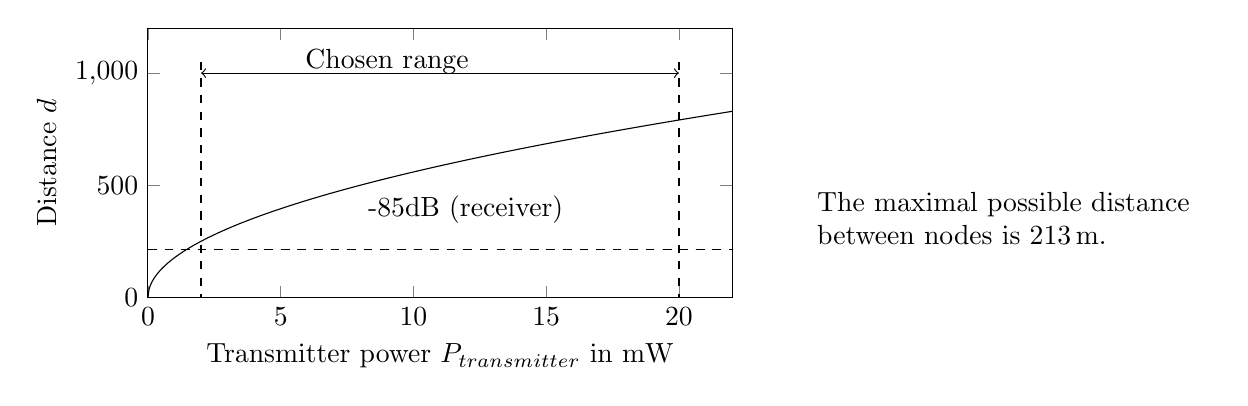
\begin{tikzpicture}
\begin{axis}[
    xmin = 0, xmax = 22,
    ymin = 0, ymax = 1200.0, samples=500, xlabel={Transmitter power $P_{transmitter}$ in mW},
        ylabel={Distance $d$}, height=5cm, width=9cm]
    \addplot[        domain = 0:22
    ] {sqrt(x/0.00000000316)*299792358/(4*pi*2400000000)} node[right,pos=0.6,yshift=-0.3cm]{-85dB (receiver)}; % -85dBm    
      \addplot[dashed, domain = 0:25,] {213} node[right,pos=0.8]{}; % -80dBm
     \draw[<->] (2,1000) -- (20,1000); 
     \draw[dashed] (2,1050) -- (2,0); 
     \draw[dashed] (20,1050) -- (20,0); 
\end{axis}
 \node[text width=5cm] at (11,1) {The maximal possible distance between nodes is 213\,m.  }; 
  \node[text width=5cm] at (4.5,3) {Chosen range }; 

\end{tikzpicture}
\caption[Damping over distance for mobile connections]{Range over the transmitter power according to the formula~\eqref{eq:friis}. The greater the transmitter power, the greater the range. With a transmitter power of 2\,mW, the range is already 250\,m. The maximum distance is 213\,m. Therefore all nodes are in coverage for a transmitter power $>2$\,mW. }
\label{fig:pathlossfriis}
\end{figure}

\chapter{Effect of network traffic (Section 4.1)}
\label{sec:effectofnetworktraffic}
The study presented here is similar to the study in Section~\ref{sec:infoverbreitung} and is based on the publication \cite{mayr-2021-com}. Code and data associated to the study can be found in the repository \url{https://github.com/pedestrian-dynamics-HM/crownet-uq-analysis}.
The scenario of this study is similar to the scenario presented in Section~\ref{sec:infoverbreitung} with three exceptions:

\begin{itemize}
\item the relay node is not shadowed by walls. 
\item network traffic is present. 
\item the arrivals follow an negative exponential distribution. 
\end{itemize} 


\begin{figure}[hbt]
\centering
\includegraphics[width=13.5cm]{./appendix/trafficInfluence/Figure10}%
\caption[Scenario for investigating the effect of network traffic]{ Scenario for investigating the effect of network traffic. 
Scenario similar to the scenario introduced in Sec.~\ref{sec:infoverbreitung}, see Fig.~\ref{fig:InfoDissSzenario} with exceptions. The position of the node that starts to disseminate detour information differs from the scenario presented in Section~\ref{sec:infoverbreitung}.  In Section~\ref{sec:infoverbreitung} the node is next to the closed gate. In the publication the node is close to arrival area. Also there is network traffic present. Figure taken from my publication~\cite{mayr-2021-com}. }
\label{fig:scenarioOldVersionWithtraffic}%
\end{figure}


In the publication~\cite{mayr-2021-com} I conduct a parameter study. I vary three model parameters and investigate their effect on the information dissemination in a WLAN ad hoc network (IEEE 802.11p).
The first parameter is the number of agents $n$, see Table~\ref{tab:parameter}. Each agent represents a mobile node in the mobile network. The network is continuously changing,
due to the agents' motion,
and so is the information dissemination through the network. A truncated exponential distribution is used for the number of agents with lower bound $lb=10$ and upper bound $ub=2000$:
\begin{equation}
n(x,b) = \frac{e^{-x}} {1-e^{b}} % f(n,b)
\label{eq:expon}
\end{equation}
I use $b=4$, shift the distribution by $lb=10$ and scale it by $ ( ub-lb ) / b $. A histogram for 2000  samples is depicted in Fig.~\ref{fig:histNum}. The type of distribution is suited to capture the rare event of shadowing that occurs randomly when the number of agents is low. Also,  an exponential distribution, while probably not often completely correct, matches certain arrival situations in a train station sufficiently well for our investigation. 



\begin{figure}[H]
\centering
\includegraphics[height=6cm]{./appendix/trafficInfluence/Figure13}%
\caption[Parameter number of agents: histogram]{Parameter number of agents: histogram. I generate it from a negative exponential distribution. I draw many  samples where $n$ is small to detect the effect of shadowing. Figure from my publication~\cite{mayr-2021-com}.}
\label{fig:histNum}%
\end{figure}%

The second parameter is the radio transmitter power $p$ which affects how far
agents can communicate. If the power is low, messages only reach agents that are
close by. Information dissemination over large distances fails (\lq
range-problem\rq). The reception in the deployed model is based on the
signal to interference plus noise (SINR) ratio. If the SINR of a given
transmission exceeds a threshold, the transmission is correctly received. I choose a threshold of {of} 6\,dB to be on the safe side (typically 4dB are used as default). Furthermore, I assume that
the radio transmitter power is equal and constant for all mobile phones within a  sample. This is a
simplification since in reality, $p$ depends on the
local situation and the device itself. I vary the transmitter power in the range 0.5\,\dots\,2.0\,mW Equivalent Isotropically Radiated Power (EIRP).

The third parameter is the network load caused by other apps. While traveling people listen to music, use navigation apps, check their emails.  Some even watch movies while walking. To make the simulation more realistic, I assume that agents use apps which produce load in the range of $ 0... 0.20$\,MB/s. This range contains listening to music ($0.01 ... 0.03$\,MB/s), using navigation apps ($0.05$\,MB/s) and even streaming videos in low-quality ($0.06$\,MB/s).
The load ${tr}$ depends on the packet inter-transmission interval $d_{tx}$ and the packet size $s_d$ \begin{equation}
{tr} = s_d \frac{1} {d_{tx}}
\label{eq:trafSize}
\end{equation}
A constant inter-transmission interval is used assuming one-packet messages. I control the packet size $s_d$ to vary the amount of load in the model. The inter-transmission interval $d_{tx}$ is defined by the (re-)broadcast interval, which is fixed to $20$\,ms. The corresponding packet size $s_d$ is between $0 ... 4000$\,B. I expect that the information dissemination might be disturbed if the network load is high.


\begin{table}[H]
\begin{footnotesize}
\begin{tabular}{@{}llrrl@{}}%
\toprule
Parameter                        & Unit & Lower bound & Upper bound & Distribution                                    type \\ \midrule
Number of agents $n$ & 1    & 10          & 2000      & Truncated exponential (Eq.~\ref{eq:expon})  \\
Transmitter power $p$      & mW   & 0.5         & 2.0       & Uniform   \\
Packet size $s_d$        & B    & 0           & 4000        & Uniform  \\
\bottomrule 
\end{tabular}%
\end{footnotesize}
\begin{footnotesize}

\bigskip
\noindent

\begin{tabular}{@{}llllll@{}}
\toprule
Dependent parameter & Equation & Unit & Lower Bound & Upper bound & Distribution \\ \midrule
Network load ${tr}$    & see Eq.~\ref{eq:trafSize}           & MB/s    & 0          & 0.20      & Uniform                                             \\ \bottomrule
\end{tabular}
\end{footnotesize}
\caption[Uncertain parameters in the network traffic study]{Uncertain parameters in the network traffic study. I want to to know how three uncertain parameters affect the dissemination time $t_{diss}$. The packet size $s_d$ controls the amount of network load ${tr}$.}%
\label{tab:parameter}%
\end{table}%

I run $20$ simulations in parallel on a server with $80$ i7 Intel cores and $250$\,GB RAM. The simulation of $2000$ samples takes more than $6$ days including two restarts of the script that manages the simulations in parallel.

\subsection*{Effect of shadowing and network load}%
\label{sec:simulationResults}

Fig.~\ref{fig:scatter} (left) depicts that information is disseminated quickly ($t_{diss}<10s$) when the number of agents exceeds $n\approx500$. The higher the network traffic that is indicated by the message size, the longer it takes to disseminate information, see Fig.~\ref{fig:scatter} (right). Fig.~\ref{fig:subresults} shows the combined effect of shadowing with network load. When shadowing occurs, agents communicate irregularly and only for short periods. If network load is present during these periods, the information spread can be impeded. The effect seems to vanish, if the number of agents is large enough, and communication is possible at any time. 


\begin{figure}[hbt!]
\centering
\includegraphics[width=\textwidth]{./appendix/trafficInfluence/Figure14}%
\caption[Dissemination time over the three parameters]{Dissemination time $t_{diss}$ in dependency of the number of agents (left), the transmitter power (middle), and the packet size (right) that is proportional to the network load. Only $1.1$\,\% of the data points exceed the $30$\,s-border. Note: The sample values of the two remaining parameters have been projected in the plane. Figure taken from my publication~\cite{mayr-2021-com}. }%
\label{fig:scatter}%
\end{figure}

\begin{figure}[H]
\centering
\includegraphics[width=14cm]{./appendix/trafficInfluence/Figure22}%
\caption[Simulations with delayed information dissemination times]{Simulations with delayed information dissemination times. Network load can lead to high dissemination times. Figure taken from my publication~\cite{mayr-2021-com}.}%
\label{fig:subresults}%
\end{figure}%









\chapter{Capacity estimation (Section 4.2)}
\label{sec:capacityestimation}
To estimate the minimum compliance necessary to avoid congestion in Section~\ref{sec:umleitalgorithmen}, I employ the jamming criterion that requires the capacity of bottleneck. The capacity can be either measured using a fundamental diagram or taken from handbooks. 
Fig. depicts the fundamental diagram of the scenario presented in Section~\ref{sec:umleitalgorithmen}. The densities and velocities were measured in the short route. The specific flow $J_S$ was computed using the relationship between density $d$ and velocity $v$ $J_S=d v $. One observes that the maximum flow is $J_C=1.58 ped/(ms)$, see Fig.~\ref{fig:capaestimateion}.
This value is higher than values from handbooks: Weidmann~\cite{weidmann-1994-cdyn} proposes a value of $1.23 ped/(ms)$, Fruin \cite{fruin-1964-cdyn} proposes $1.43 ped/(ms)$, while the SFPE handbook~\cite{hurley-2016-cdyn} provides a value of $1.30 ped/(ms)$. I think that this peak value is an overestimation of the actual flow caused by the small measurement interval of 0.4s. The average value computed with a polynomial regression model is much lower with $J_C=1.30 ped/(ms)$ which is in line with the handbook values. Therefore, I use a capacity of $J_C=1.30 ped/(ms)$ in my flow estimations.



\begin{figure}[hbt!]
\includegraphics[width=\textwidth]{../figures/appendix/capacityestimation.png} 
\caption[Fundamental diagrams for the short route]{Fundamental diagrams for the short route. The specific flow is $J_S=\rho v $. The maximum flow is $J_C=1.58 ped/(ms)$. Image as in the publication~\cite{mayr-2022-cdyn}}
\label{fig:capaestimateion}
\end{figure}


 



\chapter{Online survey: ethical approval (Section 4.3)}
\label{sec:ethicalapproval}

Ethical approval for the online survey was obtained by the Ethics Committee of Hochschule München University of Applied Sciences (Germany, Munich). The approval comprising the conduction of the survey and the publishing of results. It was approved on 10 August 2021.


\includepdf[]{./appendix/Approval.pdf}



\chapter{Online survey: collection of statistical tests (Section 4.3)}
\label{sec:collectiontables}
The following tables contain data from statistical tests and mean values that I refer to in Section~\ref{sec:reaction}. I have published the tables as supplementary material together with my publication~\cite{mayr-2023-cdyn}. They are available online under \url{https://doi.org/10.1371/journal.pone.0284540.s004}.


\begin{table}[H]
\begin{tabular}{llrrrr}
\multicolumn{6}{c}{\textbf{Prior to information}}\\                                                                                                                                         
  \hline
Route & Group &\multicolumn{3}{l}{Route attractiveness}                                                                                                                                            &  \\ 
 &  &mean & median & std & sample size \\
  \hline
 Long & Fan & 2.124 & 2 & 0.989 & 921 \\ 
  Medium & Fan & 2.904 & 3 & 1.068 & 921 \\ 
  Short & Fan & 4.636 & 5 & 0.807 & 921 \\ 
 Long & Student \& faculty associate & 2.128 & 2 & 1.038 & 444 \\ 
  Medium & Student \& faculty associate  & 2.631 & 2 & 1.042 & 444 \\ 
Short & Student \& faculty associate  & 4.732 & 5 & 0.700 & 444 \\ 
   \hline
\end{tabular}
\caption[]{Route attractiveness prior to information (5-Point Likert scale). Two surveys were conducted: one with students \& and faculty associates and one with football fans.
For each route, participants were asked how likely it is that they take the respective route when no route recommendation is provided. Since no information is provided, the message design does not have any effect (see Tab.~\ref{tab:surveyS2G}).}
\label{tab:surveyS2E}
\end{table}


\begin{table}[H]
\begin{tabular}{llrrr}
  \hline
Comparison of attractiveness & Group & Z & $p$  \\ 
  \hline
Long route and Medium route & Fan &  -11.6806 & 0.0000  \\ 
Long route and Short route & Fan &  -38.0125 & 0.0000  \\ 
 Medium route and Short route &Fan &  -26.3319 & 0.0000  \\ 
  Long route and Medium route & Student \& faculty associate &  -5.4089 & 0.0000  \\ 
 Long route and Short route & Student \& faculty associate &  -26.3982 & 0.0000  \\ 
 Medium route and Short route & Student \& faculty associate &  -20.9893 & 0.0000 \\ 
   \hline
\end{tabular}
\caption{ Route preference prior to information. For each group, the route attractiveness of the short, medium and long route differ significantly (Dunn's test). In every comparison, the shorter route is preferred ($Z < 0$).
I conclude that there is a clear route preference: the short route is favored over the medium route followed by long route (see also the mean values from Tab.~\ref{tab:surveyS2E}).}
\label{tab:surveyS2F}
\end{table}


\begin{table}[H]
\centering
\begin{tabular}{lllrrr}
\multicolumn{6}{c}{\textbf{Information provided}}\\                                                                                                                                         

  \hline
Information & Route & Group & \textit{p} & $H$ & \textit{df} \\ 
  \hline
Prior to information &  Fans & Long &   4.5498 &      0.7150 &     7 \\ 
Prior to information &   Fans & Medium &    9.4997 &      0.2190  &     7 \\ 
Prior to information &   Fans & Short &   6.5020 &     0.4820 &     7 \\ 
Prior to information &   Students \& faculty associates & Long &          0.5950  & 5.5312 & 7 \\ 
Prior to information &   Students \& faculty associates & Medium &        0.8430 &  3.4222 & 7\\ 
Prior to information &   Students \& faculty associates & Short &         0.3660 &  7.6299 & 7 \\ 
  \hline 
After receiving information &      Fans & Long & 0.0022 & 22.42 &     7 \\ 
After receiving information &  Fans & Medium & 0.0000 & 33.04 &     7 \\ 
After receiving information &    Fans & Short & 0.0000 & 95.76 &     7 \\ 
After receiving information &  Students \& faculty associates & Long & 0.8010 & 3.811 &     7 \\ 
After receiving information &   Students \& faculty associates & Medium & 0.0000 & 32.38 &     7 \\ 
After receiving information &    Students \& faculty associates & Short& 0.0000 & 45.35 &     7 \\ 
\hline   
\end{tabular}
\caption{ Effect of message design on route attractiveness (Kruskal Wallis test). Prior to information (Tab.~\ref{tab:surveyS2E}), the message design has no effect ($p>0.05$). When information is provided (Tab.~\ref{tab:surveyS2H}), the message design has an effect ($p\leq0.05$) except for the attractiveness of the long route for the student \& faculty associate group.}
\label{tab:surveyS2G}
\end{table}

\begin{table}[H]
\begin{scriptsize}
\begin{tabular}{lllrrrr}
\multicolumn{6}{c}{\textbf{After receiving information}}\\                                                                                                                                           
  \hline
Route & Group & Message design & \multicolumn{3}{l}{Route attractiveness}                                                                                                                                            &  \\ 
 &  & &mean & median & std & n \\
 \hline
 Long & Fan & Arrow & 3.427 & 4 & 1.340 & 143 \\
   Long & Fan & Arrow + team spirit & 3.553 & 4 & 1.194 & 103 \\
   Long & Fan & Arrow + top down view & 3.550 & 4 & 1.270 & 111 \\
   Long & Fan & Arrow + top down view + team spirit & 3.743 & 4 & 1.259 & 136 \\
   Long & Fan & Congestion info + arrow & 3.505 & 4 & 1.298 & 103 \\
   Long & Fan & Congestion info + arrow + team spirit & 3.980 & 4 & 1.219 & 102 \\
   Long & Fan & Congestion info + arrow + top down view & 3.897 & 4 & 1.160 & 116 \\
   Long & Fan & Congestion info + arrow + top down view + team spirit & 3.879 & 4 & 1.079 & 107 \\
   Medium & Fan & Arrow & 3.266 & 4 & 1.156 & 143 \\
   Medium & Fan & Arrow + team spirit & 3.078 & 3 & 1.135 & 103 \\
   Medium & Fan & Arrow + top down view & 3.207 & 4 & 1.113 & 111 \\
   Medium & Fan & Arrow + top down view + team spirit & 3.066 & 3 & 1.206 & 136 \\
   Medium & Fan & Congestion info + arrow & 3.534 & 4 & 1.119 & 103 \\
   Medium & Fan & Congestion info + arrow + team spirit & 3.539 & 4 & 1.158 & 102 \\
   Medium & Fan & Congestion info + arrow + top down view & 3.655 & 4 & 1.039 & 116 \\
   Medium & Fan & Congestion info + arrow + top down view + team spirit & 3.542 & 4 & 1.093 & 107 \\
   Short & Fan & Arrow & 3.643 & 4 & 1.286 & 143 \\
   Short & Fan & Arrow + team spirit & 3.786 & 4 & 1.311 & 103 \\
   Short & Fan & Arrow + top down view & 3.414 & 4 & 1.254 & 111 \\
   Short & Fan & Arrow + top down view + team spirit & 3.265 & 3 & 1.312 & 136 \\
   Short & Fan & Congestion info + arrow & 2.806 & 2 & 1.329 & 103 \\
   Short & Fan & Congestion info + arrow + team spirit & 2.471 & 2 & 1.224 & 102 \\
   Short & Fan & Congestion info + arrow + top down view & 2.784 & 2 & 1.357 & 116 \\
   Short & Fan & Congestion info + arrow + top down view + team spirit & 2.757 & 2 & 1.265 & 107 \\
   Long & Student* & Arrow & 3.787 & 4 & 1.178 & 47 \\
   Long & Student* & Arrow + team spirit & 3.696 & 4 & 1.190 & 56 \\
   Long & Student* & Arrow + top down view & 3.938 & 4 & 1.158 & 65 \\
   Long & Student* & Arrow + top down view + team spirit & 3.823 & 4 & 1.048 & 62 \\
   Long & Student* & Congestion info + arrow & 3.862 & 4 & 1.146 & 58 \\
   Long & Student* & Congestion info + arrow + team spirit & 3.700 & 4 & 1.282 & 50 \\
   Long & Student* & Congestion info + arrow + top down view & 4.022 & 4 & 1.033 & 45 \\
   Long & Student* & Congestion info + arrow + top down view + team spirit & 3.885 & 4 & 1.305 & 61 \\
   Medium & Student* & Arrow & 2.872 & 2 & 1.191 & 47 \\
   Medium & Student* & Arrow + team spirit & 2.946 & 3 & 1.052 & 56 \\
   Medium & Student* & Arrow + top down view & 2.769 & 2 & 1.129 & 65 \\
   Medium & Student* & Arrow + top down view + team spirit & 2.903 & 3 & 1.197 & 62 \\
   Medium & Student* & Congestion info + arrow & 3.483 & 4 & 1.246 & 58 \\
   Medium & Student* & Congestion info + arrow + team spirit & 3.620 & 4 & 1.276 & 50 \\
   Medium & Student* & Congestion info + arrow + top down view & 3.622 & 4 & 1.134 & 45 \\
   Medium & Student* & Congestion info + arrow + top down view + team spirit & 3.246 & 4 & 1.247 & 61 \\
   Short & Student* & Arrow & 3.128 & 3 & 1.172 & 47 \\
   Short & Student* & Arrow + team spirit & 3.321 & 4 & 1.162 & 56 \\
   Short & Student* & Arrow + top down view & 3.338 & 3 & 1.314 & 65 \\
   Short & Student* & Arrow + top down view + team spirit & 3.403 & 3 & 1.221 & 62 \\
   Short & Student* & Congestion info + arrow & 2.483 & 2 & 1.047 & 58 \\
   Short & Student* & Congestion info + arrow + team spirit & 2.540 & 2 & 1.199 & 50 \\
   Short & Student* & Congestion info + arrow + top down view & 2.533 & 2 & 1.198 & 45 \\
   Short & Student* & Congestion info + arrow + top down view + team spirit & 2.689 & 2 & 1.218 & 61 \\
   \hline
\end{tabular}
\end{scriptsize}
\caption{Route attractiveness when recommending the long route (5-Point Likert scale). Two surveys were conducted: one with students \&  faculty associates (student*) and one with football fans.
For each route, participants were asked how likely it is that they take the respective route when a route recommendation is provided. The message design always has an effect on the attractiveness of the routes except for the attractiveness of the long route, see Kruskal Wallis tests (see Tab.~\ref{tab:surveyS2G}).}
\label{tab:surveyS2H}
\end{table}




\pagestyle{empty}

\begin{sidewaystable}
\begin{scriptsize}

\hspace{-3.0cm}
\begin{tabular}{llllrr}
\multicolumn{6}{c}{\textbf{Students \& faculty associates}} \\
\hline
 Route & Added component & Message design 1 & Message design 2 & \textit{p} &  \textit{W} \\ 
  \hline
Long & Congestion info & Arrow (mean = 3.787) & Congestion info + arrow (mean = 3.862) & 0.7592 & 1317.5 \\ 
  Long & Congestion info & Arrow + top down view (mean = 3.938) & Congestion info + arrow + top down view (mean = 4.022) & 0.8557 & 1434.0 \\ 
  Long & Congestion info & Arrow + team spirit (mean = 3.696) & Congestion info + arrow + team spirit (mean = 3.700) & 0.8356 & 1368.0 \\ 
  Long & Congestion info & Arrow + top down view + team spirit (mean = 3.823) & Congestion info + arrow + top down view + team spirit (mean = 3.885) & 0.3327 & 1708.5 \\ 
  Long & Team spirit & Congestion info + arrow (mean = 3.862) & Congestion info + arrow + team spirit (mean = 3.700) & 0.6071 & 1530.0 \\ 
  Long & Team spirit & Congestion info + arrow + top down view (mean = 4.022) & Congestion info + arrow + top down view + team spirit (mean = 3.885) & 0.9810 & 1376.5 \\ 
  Long & Team spirit & Arrow (mean = 3.787) & Arrow + team spirit (mean = 3.696) & 0.6422 & 1383.5 \\ 
  Long & Team spirit & Arrow + top down view (mean = 3.938) & Arrow + top down view + team spirit (mean = 3.823) & 0.3331 & 2205.5 \\ 
  Long & Top down view & Congestion info + arrow (mean = 3.862) & Congestion info + arrow + top down view (mean = 4.022) & 0.5715 & 1224.5 \\ 
  Long & Top down view & Congestion info + arrow + team spirit (mean = 3.700) & Congestion info + arrow + top down view + team spirit (mean = 3.885) & 0.3818 & 1384.5 \\ 
  Long & Top down view & Arrow (mean = 3.787) & Arrow + top down view (mean = 3.938) & 0.4979 & 1418.5 \\ 
  Long & Top down view & Arrow + team spirit (mean = 3.696) & Arrow + top down view + team spirit (mean = 3.823) & 0.6822 & 1663.0 \\ 
  \hline
  Medium & Congestion info & Arrow (mean = 2.872) & Congestion info + arrow (mean = 3.483) & \textbf{0.0117} & 989.0 \\ 
  Medium & Congestion info & Arrow + top down view (mean = 2.769) & Congestion info + arrow + top down view (mean = 3.622) & \textbf{0.0003} & 884.5 \\ 
  Medium & Congestion info & Arrow + team spirit (mean = 2.946) & Congestion info + arrow + team spirit (mean = 3.620) & \textbf{0.0031} & 949.5 \\ 
  Medium & Congestion info & Arrow + top down view + team spirit (mean = 2.903) & Congestion info + arrow + top down view + team spirit (mean = 3.246) & 0.1243 & 1598.5 \\ 
  Medium & Team spirit & Congestion info + arrow (mean = 3.483) & Congestion info + arrow + team spirit (mean = 3.62) & 0.4871 & 1341.0 \\ 
  Medium & Team spirit & Congestion info + arrow + top down view (mean = 3.622) & Congestion info + arrow + top down view + team spirit (mean = 3.246) & 0.1283 & 1601.5 \\ 
  Medium & Team spirit & Arrow (mean = 2.872) & Arrow + team spirit (mean = 2.946) & 0.6933 & 1259.5 \\ 
  Medium & Team spirit & Arrow + top down view (mean = 2.769) & Arrow + top down view + team spirit (mean = 2.903) & 0.5484 & 1895.5 \\ 
  Medium & Top down view & Congestion info + arrow (mean = 3.483) & Congestion info + arrow + top down view (mean = 3.622) & 0.6519 & 1240.0 \\ 
  Medium & Top down view & Congestion info + arrow + team spirit (mean = 3.62) & Congestion info + arrow + top down view + team spirit (mean = 3.246) & 0.1017 & 1792.5 \\ 
  Medium & Top down view & Arrow (mean = 2.872) & Arrow + top down view (mean = 2.769) & 0.6865 & 1593.0 \\ 
  Medium & Top down view & Arrow + team spirit (mean = 2.946) & Arrow + top down view + team spirit (mean = 2.903) & 0.7897 & 1783.5 \\ 
  \hline
  Short & Congestion info & Arrow (mean = 3.128) & Congestion info + arrow (mean = 2.483) & \textbf{0.0019} & 1804.0 \\ 
  Short & Congestion info & Arrow + top down view (mean = 3.338) & Congestion info + arrow + top down view (mean = 2.533) & \textbf{0.0009} & 1974.5 \\ 
  Short & Congestion info & Arrow + team spirit (mean = 3.321) & Congestion info + arrow + team spirit (mean = 2.54) & \textbf{0.0010} & 1895.5 \\ 
  Short & Congestion info & Arrow + top down view + team spirit (mean = 3.403) & Congestion info + arrow + top down view + team spirit (mean = 2.689) & \textbf{0.0011} & 2514.5 \\ 
  Short & Team spirit & Congestion info + arrow (mean = 2.483) & Congestion info + arrow + team spirit (mean = 2.54) & 0.9363 & 1438.0 \\ 
  Short & Team spirit & Congestion info + arrow + top down view (mean = 2.533) & Congestion info + arrow + top down view + team spirit (mean = 2.689) & 0.4671 & 1270.0 \\ 
  Short & Team spirit & Arrow (mean = 3.128) & Arrow + team spirit (mean = 3.321) & 0.4109 & 1196.5 \\ 
  Short & Team spirit & Arrow + top down view (mean = 3.338) & Arrow + top down view + team spirit (mean = 3.403) & 0.7408 & 1948.0 \\ 
  Short & Top down view & Congestion info + arrow (mean = 2.483) & Congestion info + arrow + top down view (mean = 2.533) & 0.9657 & 1311.0 \\ 
  Short & Top down view & Congestion info + arrow + team spirit (mean = 2.54) & Congestion info + arrow + top down view + team spirit (mean = 2.689) & 0.5119 & 1422.5 \\ 
  Short & Top down view & Arrow (mean = 3.128) & Arrow + top down view (mean = 3.338) & 0.4113 & 1393.0 \\ 
  Short & Top down view & Arrow + team spirit (mean = 3.321) & Arrow + top down view + team spirit (mean = 3.403) & 0.6679 & 1658.5 \\ 
\hline
\end{tabular}

\end{scriptsize}

\caption[]{Effect of message component on how \textbf{students \& faculty associates} evaluate the route attractiveness (Mann Whitney U test). If adding a component makes a significant difference ($p<0.05$) the corresponding \textit{p}-Value is marked bold. The mean values '(mean = ...)` represent the respective mean values of the route attractivenesses (see Tab.~\ref{tab:surveyS2H} for the full statistics of the route attractivenesses).}
\label{tab:surveyS2A}
\end{sidewaystable}


\begin{sidewaystable}
\begin{scriptsize}
\hspace{-3.0cm}
\begin{tabular}{llllrr}
\multicolumn{6}{c}{\textbf{Fans}} \\
\hline
 Route & Added component & Message design 1 & Message design 2 & \textit{p} &  \textit{W} \\ 
  \hline
Long & Congestion info & Arrow (mean = 3.427) & Congestion info + arrow (mean = 3.505) & 0.6181 & 7099.5 \\
  Long & Congestion info & Arrow + top down view (mean = 3.55) & Congestion info + arrow + top down view (mean = 3.897) & \textbf{0.0331} & 5433.0 \\
  Long & Congestion info & Arrow + team spirit (mean = 3.553) & Congestion info + arrow + team spirit (mean = 3.980) & \textbf{0.0047} & 4107.0 \\
  Long & Congestion info & Arrow + top down view + team spirit (mean = 3.743) & Congestion info + arrow + top down view + team spirit (mean = 3.879) & 0.6983 & 7076.0 \\
  Long & Team spirit & Congestion info + arrow (mean = 3.505) & Congestion info + arrow + team spirit (mean = 3.980) & \textbf{0.0069} & 4157.0 \\
  Long & Team spirit & Congestion info + arrow + top down view (mean = 3.897) & Congestion info + arrow + top down view + team spirit (mean = 3.879) & 0.6011 & 6443.0 \\
  Long & Team spirit & Arrow (mean = 3.427) & Arrow + team spirit (mean = 3.553) & 0.5517 & 7048.5 \\
  Long & Team spirit & Arrow + top down view (mean = 3.55) & Arrow + top down view + team spirit (mean = 3.743) & 0.1957 & 6856.0 \\
  Long & Top down view & Congestion info + arrow (mean = 3.505) & Congestion info + arrow + top down view (mean = 3.897) & \textbf{0.0305} & 5006.0 \\
  Long & Top down view & Congestion info + arrow + team spirit (mean = 3.980) & Congestion info + arrow + top down view + team spirit (mean = 3.879) & 0.1645 & 6028.0 \\
  Long & Top down view & Arrow (mean = 3.427) & Arrow + top down view (mean = 3.55) & 0.5125 & 7570.5 \\
  Long & Top down view & Arrow + team spirit (mean = 3.553) & Arrow + top down view + team spirit (mean = 3.743) & 0.1652 & 6299.0 \\
    \hline
  Medium & Congestion info & Arrow (mean = 3.266) & Congestion info + arrow (mean = 3.534) & 0.0731 & 6423.5 \\
  Medium & Congestion info & Arrow + top down view (mean = 3.207) & Congestion info + arrow + top down view (mean = 3.655) & \textbf{0.0021} & 5006.5 \\
  Medium & Congestion info & Arrow + team spirit (mean = 3.078) & Congestion info + arrow + team spirit (mean = 3.539) & \textbf{0.0038} & 4087.5 \\
  Medium & Congestion info & Arrow + top down view + team spirit (mean = 3.066) & Congestion info + arrow + top down view + team spirit (mean = 3.542) & \textbf{0.0022} & 5678.0 \\
  Medium & Team spirit & Congestion info + arrow (mean = 3.534) & Congestion info + arrow + team spirit (mean = 3.539) & 0.8731 & 5188.5 \\
  Medium & Team spirit & Congestion info + arrow + top down view (mean = 3.655) & Congestion info + arrow + top down view + team spirit (mean = 3.542) & 0.4670 & 6535.0 \\
  Medium & Team spirit & Arrow (mean = 3.266) & Arrow + team spirit (mean = 3.078) & 0.1820 & 8065.5 \\
  Medium & Team spirit & Arrow + top down view (mean = 3.207) & Arrow + top down view + team spirit (mean = 3.066) & 0.3322 & 8066.0 \\
  Medium & Top down view & Congestion info + arrow (mean = 3.534) & Congestion info + arrow + top down view (mean = 3.655) & 0.4556 & 5644.5 \\
  Medium & Top down view & Congestion info + arrow + team spirit (mean = 3.539) & Congestion info + arrow + top down view + team spirit (mean = 3.542) & 0.9011 & 5508.5 \\
  Medium & Top down view & Arrow (mean = 3.266) & Arrow + top down view (mean = 3.207) & 0.6396 & 8195.5 \\
  Medium & Top down view & Arrow + team spirit (mean = 3.078) & Arrow + top down view + team spirit (mean = 3.066) & 0.9352 & 7045.5 \\
  \hline
  Short & Congestion info & Arrow (mean = 3.643) & Congestion info + arrow (mean = 2.806) & \textbf{0.0000} & 9855.0 \\
  Short & Congestion info & Arrow + top down view (mean = 3.414) & Congestion info + arrow + top down view (mean = 2.784) & \textbf{0.0003} & 8143.0 \\
  Short & Congestion info & Arrow + team spirit (mean = 3.786) & Congestion info + arrow + team spirit (mean = 2.471) & \textbf{0.0000} & 7940.5 \\
  Short & Congestion info & Arrow + top down view + team spirit (mean = 3.265) & Congestion info + arrow + top down view + team spirit (mean = 2.757) & \textbf{0.0023} & 8857.5 \\
  Short & Team spirit & Congestion info + arrow (mean = 2.806) & Congestion info + arrow + team spirit (mean = 2.471) & 0.0634 & 5993.5 \\
  Short & Team spirit & Congestion info + arrow + top down view (mean = 2.784) & Congestion info + arrow + top down view + team spirit (mean = 2.757) & 0.9759 & 6192.0 \\
  Short & Team spirit & Arrow (mean = 3.643) & Arrow + team spirit (mean = 3.786) & 0.3306 & 6851.5 \\
  Short & Team spirit & Arrow + top down view (mean = 3.414) & Arrow + top down view + team spirit (mean = 3.265) & 0.3873 & 8015.0 \\
  Short & Top down view & Congestion info + arrow (mean = 2.806) & Congestion info + arrow + top down view (mean = 2.784) & 0.8446 & 6060.5 \\
  Short & Top down view & Congestion info + arrow + team spirit (mean = 2.471) & Congestion info + arrow + top down view + team spirit (mean = 2.757) & 0.0781 & 4740.5 \\
  Short & Top down view & Arrow (mean = 3.643) & Arrow + top down view (mean = 3.414) & 0.1237 & 8799.5 \\
  Short & Top down view & Arrow + team spirit (mean = 3.786) & Arrow + top down view + team spirit (mean = 3.265) & \textbf{0.0024} & 8555.5 \\
   \hline
\end{tabular}
\end{scriptsize}
\caption[]{Effect of message component on how \textbf{fans} evaluate the route attractiveness (Mann Whitney U test). If adding a component makes a significant difference ($p<0.05$) the corresponding p-Value is marked bold. The mean values '(mean = ...)` represent the respective mean values of the route attractivenesses (see Tab.~\ref{tab:surveyS2H} for the full statistics of the route attractiveness)}
\label{tab:surveyS2B}
\end{sidewaystable}


\clearpage


%Kopf- und Fußzeile
\pagestyle{fancy}
\fancyhf{}
 
%Kopfzeile mittig mit Kaptilname
%\fancyhead[C]{\textsf{\nouppercase{\leftmark}}}

\fancyhead[C]{\textsf{ {\thechapter} \nouppercase{\leftmark} }}


%\fancyhead[R]{ \includegraphics[height=1.2cm]{./pictures/hm_logo_alt} } %\input{./pictures/image.pdf_tex}  }
%Linie oben
%\renewcommand{\headrulewidth}{0.5pt}
%Fußzeile links bzw. innen
	%\fancyfoot[L]{Christina Maria Mayr}
	\fancyfoot[C]{\thepage}
%Linie unten
%\renewcommand{\footrulewidth}{0.5pt}
 
% Fußzeile auf jeder Seite - auch Kapitel und Inhaltsverzeichnis
\fancypagestyle{plain}{%
   \fancyhf{}%
	%\fancyfoot[L]{Christina Maria Mayr}
	\fancyfoot[C]{\thepage}
   \renewcommand{\headrulewidth}{0.0pt} %obere Linie ausblenden
}




\addtolength{\headheight}{\baselineskip}
\addtolength{\headheight}{0.61pt}
\addtolength{\footskip}{10pt}
\renewcommand{\headrulewidth}{0pt}% Trennlinie

\renewcommand{\chaptermark}[1]{\markboth{#1}{}}


\begin{table}
\begin{scriptsize}

\begin{tabular}{llrrcc}
\multicolumn{6}{c}{ \textbf{Students \& faculty associates: Route attractiveness (mean value)}} \\
  \hline
 Route & Condition & Prior  & Info.  & \textit{p} & \textit{W} \\
   &  &  to info. & provided &  &  \\

  \hline
 Long & Arrow + top down view & 2.062 & 3.938 & \textbf{0.0000} & 3654.5 \\ 
   Long & Arrow + team spirit & 2.196 & 3.696 & \textbf{0.0000} & 2542.5 \\ 
   Long & Congestion info + arrow & 2.241 & 3.862 & \textbf{0.0000} & 2758.0 \\ 
   Long & Arrow + top down view + team spirit & 2.145 & 3.823 & \textbf{0.0000} & 3245.5 \\ 
   Long & Arrow & 2.149 & 3.787 & \textbf{0.0000} & 1834.0 \\ 
   Long & Congestion info + arrow + top down view + team spirit & 2.016 & 3.885 & \textbf{0.0000} & 3133.5 \\ 
   Long & Congestion info + arrow + top down view & 2.311 & 4.022 & \textbf{0.0000} & 1720.5 \\ 
   Long & Congestion info + arrow + team spirit & 1.940 & 3.700 & \textbf{0.0000} & 2105.0 \\ 
   \hline
   Medium & Arrow + top down view & 2.708 & 2.769 & 0.7852 & 2168.0 \\ 
   Medium & Arrow + team spirit & 2.643 & 2.946 & 0.1015 & 1825.5 \\ 
   Medium & Congestion info + arrow & 2.672 & 3.483 & \textbf{0.0004} & 2298.5 \\ 
   Medium & Arrow + top down view + team spirit & 2.677 & 2.903 & 0.2906 & 2122.0 \\ 
   Medium & Arrow & 2.723 & 2.872 & 0.5057 & 1185.5 \\ 
   Medium & Congestion info + arrow + top down view + team spirit & 2.607 & 3.246 & \textbf{0.0045} & 2391.0 \\ 
   Medium & Congestion info + arrow + top down view & 2.600 & 3.622 & \textbf{0.0000} & 1503.5 \\ 
   Medium & Congestion info + arrow + team spirit & 2.380 & 3.620 & \textbf{0.0000} & 1924.0 \\ 
   \hline
   Short & Arrow + top down view & 4.754 & 3.338 & \textbf{0.0000} & 847.0 \\ 
   Short & Arrow + team spirit & 4.732 & 3.321 & \textbf{0.0000} & 465.0 \\ 
   Short & Congestion info + arrow & 4.603 & 2.483 & \textbf{0.0000} & 284.0 \\ 
   Short & Arrow + top down view + team spirit & 4.806 & 3.403 & \textbf{0.0000} & 644.0 \\ 
   Short & Arrow & 4.681 & 3.128 & \textbf{0.0000} & 342.0 \\ 
   Short & Congestion info + arrow + top down view + team spirit & 4.787 & 2.689 & \textbf{0.0000} & 357.5 \\ 
   Short & Congestion info + arrow + top down view & 4.667 & 2.533 & \textbf{0.0000} & 223.0 \\ 
   Short & Congestion info + arrow + team spirit & 4.800 & 2.540 & \textbf{0.0000} & 204.0 \\ 
   \hline
\end{tabular}
\end{scriptsize}
\caption{Effect of information provision on how \textbf{students \& faculty associates} evaluate the route attractiveness (Mann Whitney U test). If information provision makes a significant difference ($p<0.05$) the corresponding \textit{p}-Value is marked bold. Through information the long route becomes always more attractive (the means increase), while the short route always becomes less attractive (the means reduce). Also, the medium route becomes more attractive. The increase of the means is not always significant.}
\label{tab:surveyS2C}
\end{table}



\begin{table}
\begin{scriptsize}
\begin{tabular}{llrrrr}
\multicolumn{6}{c}{ \textbf{Fans: Route attractiveness (mean value)}} \\
  \hline
 Route & Condition & Prior  & Info.  & \textit{p} & \textit{W} \\
   &  &  to info. & provided &  &  \\
  \hline
 Long & Arrow + top down view & 2.207 & 3.550 & \textbf{0.0000} & 9524.0 \\ 
 Long & Arrow + team spirit & 2.146 & 3.553 & \textbf{0.0000} & 8471.5 \\ 
 Long & Congestion info + arrow & 1.981 & 3.505 & \textbf{0.0000} & 8584.5 \\ 
 Long & Arrow + top down view + team spirit & 2.125 & 3.743 & \textbf{0.0000} & 15171.0 \\ 
 Long & Arrow & 2.035 & 3.427 & \textbf{0.0000} & 15846.0 \\ 
 Long & Congestion info + arrow + top down view + team spirit & 2.131 & 3.879 & \textbf{0.0000} & 9755.0 \\ 
 Long & Congestion info + arrow + top down view & 2.259 & 3.897 & \textbf{0.0000} & 11034.0 \\ 
 Long & Congestion info + arrow + team spirit & 2.118 & 3.980 & \textbf{0.0000} & 8914.0 \\ 
 \hline
 Medium & Arrow + top down view & 2.793 & 3.207 & \textbf{0.0053} & 7424.5 \\ 
 Medium & Arrow + team spirit & 2.816 & 3.078 & 0.0991 & 5969.0 \\ 
 Medium & Congestion info + arrow & 2.718 & 3.534 & \textbf{0.0000} & 7383.0 \\ 
 Medium & Arrow + top down view + team spirit & 3.029 & 3.066 & 0.8674 & 9352.0 \\ 
 Medium & Arrow & 2.909 & 3.266 & \textbf{0.0045} & 12116.5 \\ 
 Medium & Congestion info + arrow + top down view + team spirit & 3.028 & 3.542 & \textbf{0.0005} & 7214.5 \\ 
 Medium & Congestion info + arrow + top down view & 2.974 & 3.655 & \textbf{0.0000} & 8926.5 \\ 
 Medium & Congestion info + arrow + team spirit & 2.922 & 3.539 & \textbf{0.0001} & 6799.5 \\ 
 \hline
 Short & Arrow + top down view & 4.523 & 3.414 & \textbf{0.0000} & 2913.5 \\ 
 Short & Arrow + team spirit & 4.670 & 3.786 & \textbf{0.0000} & 3165.0 \\ 
 Short & Congestion info + arrow & 4.583 & 2.806 & \textbf{0.0000} & 1690.5 \\ 
 Short & Arrow + top down view + team spirit & 4.669 & 3.265 & \textbf{0.0000} & 3666.5 \\ 
 Short & Arrow & 4.692 & 3.643 & \textbf{0.0000} & 5235.0 \\ 
 Short & Congestion info + arrow + top down view + team spirit & 4.654 & 2.757 & \textbf{0.0000} & 1507.5 \\ 
 Short & Congestion info + arrow + top down view & 4.560 & 2.784 & \textbf{0.0000} & 2294.0 \\ 
 Short & Congestion info + arrow + team spirit & 4.725 & 2.471 & \textbf{0.0000} & 935.5 \\ 
   \hline
\end{tabular}
\end{scriptsize}
\caption{Effect of information provision on how \textbf{football fans} evaluate the route attractiveness (Mann Whitney U test). If information provision makes a significant difference ($p<0.05$) the corresponding \textit{p}-Value is marked bold. Through information the long route becomes always more attractive (the means increase), while the short route always becomes less attractive (the means reduce). Also, the medium route becomes more attractive. The increase of the means is not always significant.}
\label{tab:surveyS2D}
\end{table}



\chapter{Familiarity with environment (Section 4.3)}
\label{sec:navigation}

Findings from the online survey strongly indicate that people are basically willing to follow instructions provided by mobile applications. However, the survey assumed that people are familiar with the environment.
To find out how well people can follow the recommendation under real environmental conditions, I am conducting an on-site survey at the metro station Münchner Freiheit (Munich, Germany).
The survey was conducted by Christina Mayr as part of the \textit{roVer} project on 26 September 2023 (14:00-15:00) at the surface level of the train station. The procedure was as follows:
\begin{itemize}
\item Approach people (say: I'm from Munich University of Applied Sciences and I'm conducting a scientific survey together with MVG. One question for you - it will only take 10 seconds.)
\item Then show the picture (see fig.~\ref{fig:msg}) on a tablet and ask: "How well can you find the way. Please rate with a school grade."
\item Note the school grade.
\end{itemize}
18 people took part in the survey. 17 out of 18 people provided an answer. 11 out of 17 people provided information on their local knowledge without being asked.

\begin{figure}[hbt!]
\centering
\includegraphics[width=8cm]{../figures/appendix/onsite.png} 
\caption[Message design]{Message design}
\label{fig:msg}
\end{figure}


The survey indicates that people familiar with the area can easily find the recommended route, see Fig.~\ref{fig:familair}. All 6 people with local knowledge gave the school grade "very good" (1). People who are not familiar with the area have problems finding the route (rating: 4 or 5). However, 2 out of 5 people found the non-recommended direct route thanks to the signposting on site. These two people also stated that they would find it helpful if the suggested route was signposted. No tendency can be observed for people who did not indicate their local knowledge. 2 out of 6 people found it easy to find the route ("very good"). 2 out of 6 people think that finding the route is challenging ("satisfactory"). 2 out of 6 people find it difficult (grade 4 or 6).

The survey sample was small and is not representative. For a representative study, a much larger number of survey participants would be necessary, as well as the recording of other factors such as day of the week, time of day, age distribution, etc. 
Nevertheless, a tendency can already be identified from this small sample. People who are familiar with the area seem to have no problems finding the recommended route. People who are not familiar with the area may have problems finding their way. 
One way to make orientation on the surface of Münchner Freiheit generally easier would be to signpost alternative routes with the aid of static signs. If an app were to be developed, orientation could be supported, for example, with a live view such as Google Maps Live View.




\begin{figure}[hbt!]
\centering
\includegraphics[width=12cm]{../figures/appendix/resultsonsite.pdf} 
\caption[Effect of familiarity on navigation]{Effect of familiarity on navigation. }
\label{fig:familair}
\end{figure}





\chapter{Pedestrian streams at Münchner Freiheit (Section 4.4)}
\label{sec:countstudy}

On 29th Oct 2020 I conducted a counting study at the metro station Münchner Freiheit (Munich, Germany). The results of the counting study will be published soon in the conference proceedings \textit{Collective Dynamics}: The title is \textit{Estimating pedestrian flows using route distributions and sparse counting data}. 
To carry out the counting experiment, I had obtained permission from the local transport provider Münchner Verkehrsgesellschaft mbH (MVG) in Munich, Germany.  Fig.~\ref{fig:intermediatefloormucfreiheit} depicts a map of the intermediate floor of the metro station.  





\begin{figure}[H]
\includegraphics[width=0.7\textwidth]{./appendix/countingExperiment/MeasurementLines.pdf} 
\includegraphics[width=0.3\textwidth]{./appendix/countingExperiment/Messstellen_Fotos_1b.pdf} 
\includegraphics[width=0.3\textwidth]{./appendix/countingExperiment/Messstellen_Fotos_2.pdf} 
\includegraphics[width=0.3\textwidth]{./appendix/countingExperiment/Messstellen_Fotos_3.pdf} 
\caption[Counting experiment: location of the measurement lines.]{Counting experiment: location of the measurement lines. Students clicked an app whenever a person crossed an imaginary line towards a certain direction. The map in the background (top) was taken from \url{https://efa.mvv-muenchen.de/sta/muenchnerfreiheit.pdf} (16th Jan. 2023). I added arrows and routes. Own photographs (bottom). }
\label{fig:intermediatefloormucfreiheit}
\end{figure}


Students counted pedestrians at various points on the intermediate floor of the station during the afternoon in three time slots of each 30 minutes.
Students clicked an app whenever a person crossed an imaginary line towards a certain direction.


\subsection*{Arrivals over time}


Fig.~\ref{fig:timeslots} depicts the results of the counting experiment. I would like to mention that the counting experiment took place  during a lull in the Covid pandemic. Hence, the measured flows might be lower than before or after the pandemic. The flow at the measurement line 1b is always larger than the flow at the other measurement line. Unfortunately, I do not know where the arrivals come from. The arrivals  measured at line 1b can either come from the bus or side entrances. One can observe that for the measurement line 1b, the number of arrivals varies over time. 


\begin{figure}[hbt!]
\centering
\includegraphics[width=\textwidth]{./appendix/countingExperiment/Day29_IN.png} 
\caption[Counting experiment: pedestrian flows over time]{Counting experiment: pedestrian flows over time}
\label{fig:timeslots}
\end{figure}




\subsection*{Estimating the probability to take the short route}
When people walk from the bus to the metro, the direct short route congestion can occur in the intermediate floor which is not visible at the surface level. I want to know how likely it it is that passengers take the short route and experience congestion. I suggest to estimate the probability from the count data. I assume that the probability to take the short route is the ratio of the flow along the short route and the in-flow:
\begin{equation}
p_{short} = \frac{flow_{short}}{flow_{in}}
\end{equation}
The in-flow is defined as the sum of all flows of arriving passengers at the surface level, that are, arrivals from the bus or tram. I assume that the inflow is  the sum of flows measured at measurement line 1b and 2. Please note that this only holds for a steady state flow and does not consider additional flows from side entrances.

Tab.~\ref{tab:appendixrouteprobscomp} shows the route choice probabilities for the short route. Please be aware that there is uncertainty in this values: there can be other flows involved from side entrances which means the values can be either higher or lower depending on the strength of the unknown side flows. Also, the counting experiment was conducted during a lull in the corona pandemic. This mostly affects the absolute flow values, but I cannot guarantee that it does not shift the distribution of pedestrians over the routes.


%One reason for this is that I can only estimate the route distributions, as no measurement data is available for the passenger flows at bus/tram stations. In addition, the route distribution depends on factors that I cannot control or measure. For example, I know the age and gender distribution from the survey, but not from the measurement data. In addition, I assume that people behave differently under real conditions than they state in the survey. For these reasons, the data are not suitable for validation. The following considerations represent a plausibility check and are not to be equated with a quantitative validation. 



\begin{table}[hbt!]
\begin{tabular}{p{2cm}p{2cm}p{2cm}p{2cm}p{2cm}p{2cm}}
\toprule
Time slot &   M-A-IN &   M-B2-IN &   M1-(EFG)-IN &   M-B-IN-cleaned &  Probability: short route \\
\midrule
14:30:00  &       43 &       111 &           302 &               68 &    0.82 \\
15:20:00  &       65 &       147 &           307 &               82 &    0.79 \\
16:05:00  &       72 &       179 &           329 &              107 &    0.75 \\
\bottomrule
\end{tabular}
\caption[Counting experiment: route probability of the short route for validation]{Counting experiment: route probability of the short route for validation. Total number of arrivals for each time slot and corresponding probability for the short route.}
\label{tab:appendixrouteprobscomp}
\end{table}

Interestingly, the probability of the short route decreases over the number of arrivals, see Fig.~\ref{fig:correlationroutechoice}. This indicates that the more people, the more congestion and the more likely people take alternative routes.  However, I cannot provide statistical evidence with only three data points.

\begin{figure}[hbt!]
\centering
\begin{tikzpicture}
\node[] at (0,0) {\includegraphics[width=7cm,trim={1cm 0 0 0},clip]{./appendix/countingExperiment/Correlation.png} };
\node[fill=white,font=\small] at (-0.2,-2.5) {370~~~~~~~~390~~~~~~~~410~~~~~~~~430};
\node[fill=white] at (0,-3.2) {Number of arrivals};
\node[fill=white,rotate=90] at (-3.4,0) {Probability: short route };
\node[] at (-2.1,1.9) {0.82};
\node[] at (-0.3,0.4) {0.79};
\node[] at (2.4,-1.4) {0.75};
\end{tikzpicture}
\caption[Estimated probability for the short route over arrivals ]{Estimated probability for the short route over arrivals. The estimated probability to take the short route decreases over the number of arrivals. }
\label{fig:correlationroutechoice}
\end{figure}

\clearpage

\newpage

\thispagestyle{empty}

{\color{white}.}

\vspace{6cm}

\begin{center}
\textit{Last page of the document}
\end{center}






\end{appendices}


\end{document}
